\documentclass[twoside]{book}

% Packages required by doxygen
\usepackage{fixltx2e}
\usepackage{calc}
\usepackage{doxygen}
\usepackage{graphicx}
\usepackage[utf8]{inputenc}
\usepackage{makeidx}
\usepackage{multicol}
\usepackage{multirow}
\PassOptionsToPackage{warn}{textcomp}
\usepackage{textcomp}
\usepackage[nointegrals]{wasysym}
\usepackage[table]{xcolor}

% Font selection
\usepackage[T1]{fontenc}
\usepackage[scaled=.90]{helvet}
\usepackage{courier}
\usepackage{amssymb}
\usepackage{sectsty}
\renewcommand{\familydefault}{\sfdefault}
\allsectionsfont{%
  \fontseries{bc}\selectfont%
  \color{darkgray}%
}
\renewcommand{\DoxyLabelFont}{%
  \fontseries{bc}\selectfont%
  \color{darkgray}%
}
\newcommand{\+}{\discretionary{\mbox{\scriptsize$\hookleftarrow$}}{}{}}

% Page & text layout
\usepackage{geometry}
\geometry{%
  a4paper,%
  top=2.5cm,%
  bottom=2.5cm,%
  left=2.5cm,%
  right=2.5cm%
}
\tolerance=750
\hfuzz=15pt
\hbadness=750
\setlength{\emergencystretch}{15pt}
\setlength{\parindent}{0cm}
\setlength{\parskip}{0.2cm}
\makeatletter
\renewcommand{\paragraph}{%
  \@startsection{paragraph}{4}{0ex}{-1.0ex}{1.0ex}{%
    \normalfont\normalsize\bfseries\SS@parafont%
  }%
}
\renewcommand{\subparagraph}{%
  \@startsection{subparagraph}{5}{0ex}{-1.0ex}{1.0ex}{%
    \normalfont\normalsize\bfseries\SS@subparafont%
  }%
}
\makeatother

% Headers & footers
\usepackage{fancyhdr}
\pagestyle{fancyplain}
\fancyhead[LE]{\fancyplain{}{\bfseries\thepage}}
\fancyhead[CE]{\fancyplain{}{}}
\fancyhead[RE]{\fancyplain{}{\bfseries\leftmark}}
\fancyhead[LO]{\fancyplain{}{\bfseries\rightmark}}
\fancyhead[CO]{\fancyplain{}{}}
\fancyhead[RO]{\fancyplain{}{\bfseries\thepage}}
\fancyfoot[LE]{\fancyplain{}{}}
\fancyfoot[CE]{\fancyplain{}{}}
\fancyfoot[RE]{\fancyplain{}{\bfseries\scriptsize Generated on Thu Nov 6 2014 17\+:13\+:46 for libsensorj by Doxygen }}
\fancyfoot[LO]{\fancyplain{}{\bfseries\scriptsize Generated on Thu Nov 6 2014 17\+:13\+:46 for libsensorj by Doxygen }}
\fancyfoot[CO]{\fancyplain{}{}}
\fancyfoot[RO]{\fancyplain{}{}}
\renewcommand{\footrulewidth}{0.4pt}
\renewcommand{\chaptermark}[1]{%
  \markboth{#1}{}%
}
\renewcommand{\sectionmark}[1]{%
  \markright{\thesection\ #1}%
}

% Indices & bibliography
\usepackage{natbib}
\usepackage[titles]{tocloft}
\setcounter{tocdepth}{3}
\setcounter{secnumdepth}{5}
\makeindex

% Hyperlinks (required, but should be loaded last)
\usepackage{ifpdf}
\ifpdf
  \usepackage[pdftex,pagebackref=true]{hyperref}
\else
  \usepackage[ps2pdf,pagebackref=true]{hyperref}
\fi
\hypersetup{%
  colorlinks=true,%
  linkcolor=blue,%
  citecolor=blue,%
  unicode%
}

% Custom commands
\newcommand{\clearemptydoublepage}{%
  \newpage{\pagestyle{empty}\cleardoublepage}%
}


%===== C O N T E N T S =====

\begin{document}

% Titlepage & ToC
\hypersetup{pageanchor=false,
             bookmarks=true,
             bookmarksnumbered=true,
             pdfencoding=unicode
            }
\pagenumbering{roman}
\begin{titlepage}
\vspace*{7cm}
\begin{center}%
{\Large libsensorj }\\
\vspace*{1cm}
{\large Generated by Doxygen 1.8.8}\\
\vspace*{0.5cm}
{\small Thu Nov 6 2014 17:13:46}\\
\end{center}
\end{titlepage}
\clearemptydoublepage
\tableofcontents
\clearemptydoublepage
\pagenumbering{arabic}
\hypersetup{pageanchor=true}

%--- Begin generated contents ---
\chapter{Namespace Index}
\section{Packages}
Here are the packages with brief descriptions (if available)\+:\begin{DoxyCompactList}
\item\contentsline{section}{\hyperlink{namespacecom}{com} }{\pageref{namespacecom}}{}
\item\contentsline{section}{\hyperlink{namespacecom_1_1libsensorj}{com.\+libsensorj} }{\pageref{namespacecom_1_1libsensorj}}{}
\item\contentsline{section}{\hyperlink{namespacecom_1_1libsensorj_1_1concreteevent}{com.\+libsensorj.\+concreteevent} }{\pageref{namespacecom_1_1libsensorj_1_1concreteevent}}{}
\item\contentsline{section}{\hyperlink{namespacecom_1_1libsensorj_1_1concretefactory}{com.\+libsensorj.\+concretefactory} }{\pageref{namespacecom_1_1libsensorj_1_1concretefactory}}{}
\item\contentsline{section}{\hyperlink{namespacecom_1_1libsensorj_1_1concretesensor}{com.\+libsensorj.\+concretesensor} }{\pageref{namespacecom_1_1libsensorj_1_1concretesensor}}{}
\item\contentsline{section}{\hyperlink{namespacecom_1_1libsensorj_1_1examples}{com.\+libsensorj.\+examples} }{\pageref{namespacecom_1_1libsensorj_1_1examples}}{}
\item\contentsline{section}{\hyperlink{namespacecom_1_1libsensorj_1_1interfaces}{com.\+libsensorj.\+interfaces} }{\pageref{namespacecom_1_1libsensorj_1_1interfaces}}{}
\item\contentsline{section}{\hyperlink{namespacecom_1_1libsensorj_1_1model}{com.\+libsensorj.\+model} }{\pageref{namespacecom_1_1libsensorj_1_1model}}{}
\item\contentsline{section}{\hyperlink{namespacecom_1_1pi4j}{com.\+pi4j} }{\pageref{namespacecom_1_1pi4j}}{}
\item\contentsline{section}{\hyperlink{namespacecom_1_1pi4j_1_1examples}{com.\+pi4j.\+examples} }{\pageref{namespacecom_1_1pi4j_1_1examples}}{}
\end{DoxyCompactList}

\chapter{Hierarchical Index}
\section{Class Hierarchy}
This inheritance list is sorted roughly, but not completely, alphabetically\+:\begin{DoxyCompactList}
\item \contentsline{section}{com.\+pi4j.\+examples.\+Blink\+Gpio\+Example}{\pageref{classcom_1_1pi4j_1_1examples_1_1BlinkGpioExample}}{}
\item \contentsline{section}{com.\+pi4j.\+examples.\+Blink\+Trigger\+Gpio\+Example}{\pageref{classcom_1_1pi4j_1_1examples_1_1BlinkTriggerGpioExample}}{}
\item \contentsline{section}{com.\+pi4j.\+examples.\+Control\+Gpio\+Example}{\pageref{classcom_1_1pi4j_1_1examples_1_1ControlGpioExample}}{}
\item \contentsline{section}{com.\+pi4j.\+examples.\+Cylon\+Gpio\+Example}{\pageref{classcom_1_1pi4j_1_1examples_1_1CylonGpioExample}}{}
\item \contentsline{section}{com.\+libsensorj.\+examples.\+D\+H\+T11\+Temperature\+Example}{\pageref{classcom_1_1libsensorj_1_1examples_1_1DHT11TemperatureExample}}{}
\item \contentsline{section}{com.\+pi4j.\+examples.\+Example}{\pageref{classcom_1_1pi4j_1_1examples_1_1Example}}{}
\item \contentsline{section}{com.\+pi4j.\+examples.\+Frequency\+Gpio\+Example}{\pageref{classcom_1_1pi4j_1_1examples_1_1FrequencyGpioExample}}{}
\item \contentsline{section}{com.\+pi4j.\+examples.\+I2\+C\+Wii\+Motion\+Plus\+Example}{\pageref{classcom_1_1pi4j_1_1examples_1_1I2CWiiMotionPlusExample}}{}
\item \contentsline{section}{com.\+libsensorj.\+interfaces.\+I\+Event}{\pageref{interfacecom_1_1libsensorj_1_1interfaces_1_1IEvent}}{}
\begin{DoxyCompactList}
\item \contentsline{section}{com.\+libsensorj.\+concreteevent.\+Humidity\+Event}{\pageref{classcom_1_1libsensorj_1_1concreteevent_1_1HumidityEvent}}{}
\item \contentsline{section}{com.\+libsensorj.\+concreteevent.\+Temperature\+Event}{\pageref{classcom_1_1libsensorj_1_1concreteevent_1_1TemperatureEvent}}{}
\item \contentsline{section}{com.\+libsensorj.\+concreteevent.\+Ultrasonic\+Range\+Finder\+Event}{\pageref{classcom_1_1libsensorj_1_1concreteevent_1_1UltrasonicRangeFinderEvent}}{}
\end{DoxyCompactList}
\item \contentsline{section}{com.\+libsensorj.\+interfaces.\+I\+Sensor}{\pageref{interfacecom_1_1libsensorj_1_1interfaces_1_1ISensor}}{}
\begin{DoxyCompactList}
\item \contentsline{section}{com.\+libsensorj.\+concretesensor.\+D\+H\+T11\+Humidity}{\pageref{classcom_1_1libsensorj_1_1concretesensor_1_1DHT11Humidity}}{}
\item \contentsline{section}{com.\+libsensorj.\+concretesensor.\+D\+H\+T11\+Temperature}{\pageref{classcom_1_1libsensorj_1_1concretesensor_1_1DHT11Temperature}}{}
\item \contentsline{section}{com.\+libsensorj.\+concretesensor.\+Ultrasonic\+Hcsr04}{\pageref{classcom_1_1libsensorj_1_1concretesensor_1_1UltrasonicHcsr04}}{}
\end{DoxyCompactList}
\item \contentsline{section}{com.\+libsensorj.\+interfaces.\+I\+Sensor\+Factory}{\pageref{interfacecom_1_1libsensorj_1_1interfaces_1_1ISensorFactory}}{}
\begin{DoxyCompactList}
\item \contentsline{section}{com.\+libsensorj.\+concretefactory.\+Humidity\+Sensor\+Factory}{\pageref{classcom_1_1libsensorj_1_1concretefactory_1_1HumiditySensorFactory}}{}
\item \contentsline{section}{com.\+libsensorj.\+concretefactory.\+Temperature\+Sensor\+Factory}{\pageref{classcom_1_1libsensorj_1_1concretefactory_1_1TemperatureSensorFactory}}{}
\item \contentsline{section}{com.\+libsensorj.\+concretefactory.\+Ultrasonic\+Range\+Finder\+Factory}{\pageref{classcom_1_1libsensorj_1_1concretefactory_1_1UltrasonicRangeFinderFactory}}{}
\end{DoxyCompactList}
\item \contentsline{section}{com.\+pi4j.\+examples.\+Lcd\+Example}{\pageref{classcom_1_1pi4j_1_1examples_1_1LcdExample}}{}
\item \contentsline{section}{com.\+pi4j.\+examples.\+Listen\+Gpio\+Example}{\pageref{classcom_1_1pi4j_1_1examples_1_1ListenGpioExample}}{}
\item \contentsline{section}{com.\+pi4j.\+examples.\+Listen\+Multiple\+Gpio\+Example}{\pageref{classcom_1_1pi4j_1_1examples_1_1ListenMultipleGpioExample}}{}
\item \contentsline{section}{com.\+pi4j.\+examples.\+M\+C\+P23017\+Gpio\+Example}{\pageref{classcom_1_1pi4j_1_1examples_1_1MCP23017GpioExample}}{}
\item \contentsline{section}{com.\+pi4j.\+examples.\+M\+C\+P23\+S17\+Gpio\+Example}{\pageref{classcom_1_1pi4j_1_1examples_1_1MCP23S17GpioExample}}{}
\item \contentsline{section}{com.\+pi4j.\+examples.\+M\+C\+P4725\+Gpio\+Example}{\pageref{classcom_1_1pi4j_1_1examples_1_1MCP4725GpioExample}}{}
\item \contentsline{section}{com.\+pi4j.\+examples.\+Multipurpose\+Pin\+Gpio\+Example}{\pageref{classcom_1_1pi4j_1_1examples_1_1MultipurposePinGpioExample}}{}
\item \contentsline{section}{com.\+pi4j.\+examples.\+My\+Example}{\pageref{classcom_1_1pi4j_1_1examples_1_1MyExample}}{}
\item \contentsline{section}{com.\+libsensorj.\+model.\+Observer}{\pageref{classcom_1_1libsensorj_1_1model_1_1Observer}}{}
\item \contentsline{section}{com.\+pi4j.\+examples.\+Olimex\+Gpio\+Example}{\pageref{classcom_1_1pi4j_1_1examples_1_1OlimexGpioExample}}{}
\item \contentsline{section}{com.\+pi4j.\+examples.\+Output\+Hi\+Gpio\+Example}{\pageref{classcom_1_1pi4j_1_1examples_1_1OutputHiGpioExample}}{}
\item \contentsline{section}{com.\+pi4j.\+examples.\+P\+C\+A9685\+Gpio\+Example}{\pageref{classcom_1_1pi4j_1_1examples_1_1PCA9685GpioExample}}{}
\item \contentsline{section}{com.\+pi4j.\+examples.\+P\+C\+A9685\+Gpio\+Servo\+Example}{\pageref{classcom_1_1pi4j_1_1examples_1_1PCA9685GpioServoExample}}{}
\item \contentsline{section}{com.\+pi4j.\+examples.\+P\+C\+F8574\+Gpio\+Example}{\pageref{classcom_1_1pi4j_1_1examples_1_1PCF8574GpioExample}}{}
\item \contentsline{section}{com.\+pi4j.\+examples.\+Pi\+Face\+Example}{\pageref{classcom_1_1pi4j_1_1examples_1_1PiFaceExample}}{}
\item \contentsline{section}{com.\+pi4j.\+examples.\+Pi\+Face\+Gpio\+Example}{\pageref{classcom_1_1pi4j_1_1examples_1_1PiFaceGpioExample}}{}
\item \contentsline{section}{com.\+pi4j.\+examples.\+R\+P\+I\+Servo\+Blaster\+Example}{\pageref{classcom_1_1pi4j_1_1examples_1_1RPIServoBlasterExample}}{}
\item \contentsline{section}{com.\+pi4j.\+examples.\+Serial\+Example}{\pageref{classcom_1_1pi4j_1_1examples_1_1SerialExample}}{}
\item \contentsline{section}{com.\+pi4j.\+examples.\+Shutdown\+Gpio\+Example}{\pageref{classcom_1_1pi4j_1_1examples_1_1ShutdownGpioExample}}{}
\item \contentsline{section}{com.\+pi4j.\+examples.\+Stepper\+Motor\+Gpio\+Example}{\pageref{classcom_1_1pi4j_1_1examples_1_1StepperMotorGpioExample}}{}
\item \contentsline{section}{com.\+pi4j.\+examples.\+System\+Info\+Example}{\pageref{classcom_1_1pi4j_1_1examples_1_1SystemInfoExample}}{}
\item Thread\begin{DoxyCompactList}
\item \contentsline{section}{com.\+pi4j.\+examples.\+P\+C\+A9685\+Gpio\+Servo\+Example.\+Sweeper}{\pageref{classcom_1_1pi4j_1_1examples_1_1PCA9685GpioServoExample_1_1Sweeper}}{}
\end{DoxyCompactList}
\item \contentsline{section}{com.\+pi4j.\+examples.\+I2\+C\+Wii\+Motion\+Plus\+Example.\+Three\+Axis}{\pageref{classcom_1_1pi4j_1_1examples_1_1I2CWiiMotionPlusExample_1_1ThreeAxis}}{}
\item \contentsline{section}{com.\+pi4j.\+examples.\+Trigger\+Gpio\+Example}{\pageref{classcom_1_1pi4j_1_1examples_1_1TriggerGpioExample}}{}
\item \contentsline{section}{com.\+libsensorj.\+examples.\+Ultrasonic\+Range\+Finder\+Example}{\pageref{classcom_1_1libsensorj_1_1examples_1_1UltrasonicRangeFinderExample}}{}
\item \contentsline{section}{com.\+pi4j.\+examples.\+Usage\+Gpio\+Example}{\pageref{classcom_1_1pi4j_1_1examples_1_1UsageGpioExample}}{}
\item \contentsline{section}{com.\+pi4j.\+examples.\+I2\+C\+Wii\+Motion\+Plus\+Example.\+Wii\+Motion\+Plus}{\pageref{classcom_1_1pi4j_1_1examples_1_1I2CWiiMotionPlusExample_1_1WiiMotionPlus}}{}
\item \contentsline{section}{com.\+pi4j.\+examples.\+Wiring\+Pi\+Gpio\+Example}{\pageref{classcom_1_1pi4j_1_1examples_1_1WiringPiGpioExample}}{}
\item \contentsline{section}{com.\+pi4j.\+examples.\+Wiring\+Pi\+Gpio\+Interrupt\+Example}{\pageref{classcom_1_1pi4j_1_1examples_1_1WiringPiGpioInterruptExample}}{}
\item \contentsline{section}{com.\+pi4j.\+examples.\+Wiring\+Pi\+Gpio\+Interrupt\+Example2}{\pageref{classcom_1_1pi4j_1_1examples_1_1WiringPiGpioInterruptExample2}}{}
\item \contentsline{section}{com.\+pi4j.\+examples.\+Wiring\+Pi\+Lcd\+Example}{\pageref{classcom_1_1pi4j_1_1examples_1_1WiringPiLcdExample}}{}
\item \contentsline{section}{com.\+pi4j.\+examples.\+Wiring\+Pi\+Serial\+Example}{\pageref{classcom_1_1pi4j_1_1examples_1_1WiringPiSerialExample}}{}
\item \contentsline{section}{com.\+pi4j.\+examples.\+Wiring\+Pi\+Soft\+P\+W\+M\+Example}{\pageref{classcom_1_1pi4j_1_1examples_1_1WiringPiSoftPWMExample}}{}
\item \contentsline{section}{com.\+pi4j.\+examples.\+Wiring\+Pi\+S\+P\+I\+Example}{\pageref{classcom_1_1pi4j_1_1examples_1_1WiringPiSPIExample}}{}
\item Gpio\+Pin\+Listener\+Digital\begin{DoxyCompactList}
\item \contentsline{section}{com.\+pi4j.\+examples.\+Usage\+Gpio\+Example.\+Gpio\+Usage\+Example\+Listener}{\pageref{classcom_1_1pi4j_1_1examples_1_1UsageGpioExample_1_1GpioUsageExampleListener}}{}
\end{DoxyCompactList}
\end{DoxyCompactList}

\chapter{Class Index}
\section{Class List}
Here are the classes, structs, unions and interfaces with brief descriptions\+:\begin{DoxyCompactList}
\item\contentsline{section}{\hyperlink{classcom_1_1libsensorj_1_1concretesensor_1_1DHT11}{com.\+libsensorj.\+concretesensor.\+D\+H\+T11} }{\pageref{classcom_1_1libsensorj_1_1concretesensor_1_1DHT11}}{}
\item\contentsline{section}{\hyperlink{classcom_1_1libsensorj_1_1concretesensor_1_1DHT11Humidity}{com.\+libsensorj.\+concretesensor.\+D\+H\+T11\+Humidity} }{\pageref{classcom_1_1libsensorj_1_1concretesensor_1_1DHT11Humidity}}{}
\item\contentsline{section}{\hyperlink{classcom_1_1libsensorj_1_1concretesensor_1_1DHT11Temperature}{com.\+libsensorj.\+concretesensor.\+D\+H\+T11\+Temperature} }{\pageref{classcom_1_1libsensorj_1_1concretesensor_1_1DHT11Temperature}}{}
\item\contentsline{section}{\hyperlink{classcom_1_1libsensorj_1_1examples_1_1DHT11TemperatureExample}{com.\+libsensorj.\+examples.\+D\+H\+T11\+Temperature\+Example} }{\pageref{classcom_1_1libsensorj_1_1examples_1_1DHT11TemperatureExample}}{}
\item\contentsline{section}{\hyperlink{classcom_1_1libsensorj_1_1concretesensor_1_1DHT11V2}{com.\+libsensorj.\+concretesensor.\+D\+H\+T11\+V2} }{\pageref{classcom_1_1libsensorj_1_1concretesensor_1_1DHT11V2}}{}
\item\contentsline{section}{\hyperlink{classcom_1_1libsensorj_1_1examples_1_1DHT11V2Example}{com.\+libsensorj.\+examples.\+D\+H\+T11\+V2\+Example} }{\pageref{classcom_1_1libsensorj_1_1examples_1_1DHT11V2Example}}{}
\item\contentsline{section}{\hyperlink{classcom_1_1libsensorj_1_1concretefactory_1_1DHT11V2Factory}{com.\+libsensorj.\+concretefactory.\+D\+H\+T11\+V2\+Factory} }{\pageref{classcom_1_1libsensorj_1_1concretefactory_1_1DHT11V2Factory}}{}
\item\contentsline{section}{\hyperlink{classcom_1_1libsensorj_1_1concretesensor_1_1DHT11V3}{com.\+libsensorj.\+concretesensor.\+D\+H\+T11\+V3} }{\pageref{classcom_1_1libsensorj_1_1concretesensor_1_1DHT11V3}}{}
\item\contentsline{section}{\hyperlink{classcom_1_1libsensorj_1_1examples_1_1DHT11V3Example}{com.\+libsensorj.\+examples.\+D\+H\+T11\+V3\+Example} }{\pageref{classcom_1_1libsensorj_1_1examples_1_1DHT11V3Example}}{}
\item\contentsline{section}{\hyperlink{classcom_1_1libsensorj_1_1concretefactory_1_1DHT11V3Factory}{com.\+libsensorj.\+concretefactory.\+D\+H\+T11\+V3\+Factory} }{\pageref{classcom_1_1libsensorj_1_1concretefactory_1_1DHT11V3Factory}}{}
\item\contentsline{section}{\hyperlink{classcom_1_1libsensorj_1_1concretesensor_1_1HCSR04Device}{com.\+libsensorj.\+concretesensor.\+H\+C\+S\+R04\+Device} }{\pageref{classcom_1_1libsensorj_1_1concretesensor_1_1HCSR04Device}}{}
\item\contentsline{section}{\hyperlink{classcom_1_1libsensorj_1_1examples_1_1HCSR04DeviceExample}{com.\+libsensorj.\+examples.\+H\+C\+S\+R04\+Device\+Example} }{\pageref{classcom_1_1libsensorj_1_1examples_1_1HCSR04DeviceExample}}{}
\item\contentsline{section}{\hyperlink{classcom_1_1libsensorj_1_1concretefactory_1_1HCSR04DeviceFactory}{com.\+libsensorj.\+concretefactory.\+H\+C\+S\+R04\+Device\+Factory} }{\pageref{classcom_1_1libsensorj_1_1concretefactory_1_1HCSR04DeviceFactory}}{}
\item\contentsline{section}{\hyperlink{classcom_1_1libsensorj_1_1concreteevent_1_1HumidityEvent}{com.\+libsensorj.\+concreteevent.\+Humidity\+Event} }{\pageref{classcom_1_1libsensorj_1_1concreteevent_1_1HumidityEvent}}{}
\item\contentsline{section}{\hyperlink{classcom_1_1libsensorj_1_1concretefactory_1_1HumiditySensorFactory}{com.\+libsensorj.\+concretefactory.\+Humidity\+Sensor\+Factory} }{\pageref{classcom_1_1libsensorj_1_1concretefactory_1_1HumiditySensorFactory}}{}
\item\contentsline{section}{\hyperlink{classcom_1_1libsensorj_1_1interfaces_1_1IEvent}{com.\+libsensorj.\+interfaces.\+I\+Event} }{\pageref{classcom_1_1libsensorj_1_1interfaces_1_1IEvent}}{}
\item\contentsline{section}{\hyperlink{interfacecom_1_1libsensorj_1_1interfaces_1_1ISensor}{com.\+libsensorj.\+interfaces.\+I\+Sensor} }{\pageref{interfacecom_1_1libsensorj_1_1interfaces_1_1ISensor}}{}
\item\contentsline{section}{\hyperlink{interfacecom_1_1libsensorj_1_1interfaces_1_1ISensorFactory}{com.\+libsensorj.\+interfaces.\+I\+Sensor\+Factory} }{\pageref{interfacecom_1_1libsensorj_1_1interfaces_1_1ISensorFactory}}{}
\item\contentsline{section}{\hyperlink{classcom_1_1libsensorj_1_1utils_1_1LibPins}{com.\+libsensorj.\+utils.\+Lib\+Pins} }{\pageref{classcom_1_1libsensorj_1_1utils_1_1LibPins}}{}
\item\contentsline{section}{\hyperlink{classcom_1_1pi4j_1_1examples_1_1MyExample}{com.\+pi4j.\+examples.\+My\+Example} }{\pageref{classcom_1_1pi4j_1_1examples_1_1MyExample}}{}
\item\contentsline{section}{\hyperlink{classcom_1_1libsensorj_1_1model_1_1Observer}{com.\+libsensorj.\+model.\+Observer} }{\pageref{classcom_1_1libsensorj_1_1model_1_1Observer}}{}
\item\contentsline{section}{\hyperlink{enumcom_1_1libsensorj_1_1utils_1_1PinNumbers}{com.\+libsensorj.\+utils.\+Pin\+Numbers} }{\pageref{enumcom_1_1libsensorj_1_1utils_1_1PinNumbers}}{}
\item\contentsline{section}{\hyperlink{classcom_1_1libsensorj_1_1concreteevent_1_1TemperatureEvent}{com.\+libsensorj.\+concreteevent.\+Temperature\+Event} }{\pageref{classcom_1_1libsensorj_1_1concreteevent_1_1TemperatureEvent}}{}
\item\contentsline{section}{\hyperlink{classcom_1_1libsensorj_1_1concretefactory_1_1TemperatureSensorFactory}{com.\+libsensorj.\+concretefactory.\+Temperature\+Sensor\+Factory} }{\pageref{classcom_1_1libsensorj_1_1concretefactory_1_1TemperatureSensorFactory}}{}
\item\contentsline{section}{\hyperlink{classcom_1_1libsensorj_1_1concretesensor_1_1UltrasonicHcsr04}{com.\+libsensorj.\+concretesensor.\+Ultrasonic\+Hcsr04} }{\pageref{classcom_1_1libsensorj_1_1concretesensor_1_1UltrasonicHcsr04}}{}
\item\contentsline{section}{\hyperlink{classcom_1_1libsensorj_1_1concreteevent_1_1UltrasonicRangeFinderEvent}{com.\+libsensorj.\+concreteevent.\+Ultrasonic\+Range\+Finder\+Event} }{\pageref{classcom_1_1libsensorj_1_1concreteevent_1_1UltrasonicRangeFinderEvent}}{}
\item\contentsline{section}{\hyperlink{classcom_1_1libsensorj_1_1examples_1_1UltrasonicRangeFinderExample}{com.\+libsensorj.\+examples.\+Ultrasonic\+Range\+Finder\+Example} }{\pageref{classcom_1_1libsensorj_1_1examples_1_1UltrasonicRangeFinderExample}}{}
\item\contentsline{section}{\hyperlink{classcom_1_1libsensorj_1_1concretefactory_1_1UltrasonicRangeFinderFactory}{com.\+libsensorj.\+concretefactory.\+Ultrasonic\+Range\+Finder\+Factory} }{\pageref{classcom_1_1libsensorj_1_1concretefactory_1_1UltrasonicRangeFinderFactory}}{}
\end{DoxyCompactList}

\chapter{File Index}
\section{File List}
Here is a list of all files with brief descriptions\+:\begin{DoxyCompactList}
\item\contentsline{section}{main/java/com/libsensorj/concreteevent/\hyperlink{HumidityEvent_8java}{Humidity\+Event.\+java} }{\pageref{HumidityEvent_8java}}{}
\item\contentsline{section}{main/java/com/libsensorj/concreteevent/\hyperlink{TemperatureEvent_8java}{Temperature\+Event.\+java} }{\pageref{TemperatureEvent_8java}}{}
\item\contentsline{section}{main/java/com/libsensorj/concreteevent/\hyperlink{UltrasonicRangeFinderEvent_8java}{Ultrasonic\+Range\+Finder\+Event.\+java} }{\pageref{UltrasonicRangeFinderEvent_8java}}{}
\item\contentsline{section}{main/java/com/libsensorj/concretefactory/\hyperlink{HumiditySensorFactory_8java}{Humidity\+Sensor\+Factory.\+java} }{\pageref{HumiditySensorFactory_8java}}{}
\item\contentsline{section}{main/java/com/libsensorj/concretefactory/\hyperlink{TemperatureSensorFactory_8java}{Temperature\+Sensor\+Factory.\+java} }{\pageref{TemperatureSensorFactory_8java}}{}
\item\contentsline{section}{main/java/com/libsensorj/concretefactory/\hyperlink{UltrasonicRangeFinderFactory_8java}{Ultrasonic\+Range\+Finder\+Factory.\+java} }{\pageref{UltrasonicRangeFinderFactory_8java}}{}
\item\contentsline{section}{main/java/com/libsensorj/concretesensor/\hyperlink{DHT11Humidity_8java}{D\+H\+T11\+Humidity.\+java} }{\pageref{DHT11Humidity_8java}}{}
\item\contentsline{section}{main/java/com/libsensorj/concretesensor/\hyperlink{DHT11Temperature_8java}{D\+H\+T11\+Temperature.\+java} }{\pageref{DHT11Temperature_8java}}{}
\item\contentsline{section}{main/java/com/libsensorj/concretesensor/\hyperlink{UltrasonicHcsr04_8java}{Ultrasonic\+Hcsr04.\+java} }{\pageref{UltrasonicHcsr04_8java}}{}
\item\contentsline{section}{main/java/com/libsensorj/examples/\hyperlink{DHT11TemperatureExample_8java}{D\+H\+T11\+Temperature\+Example.\+java} }{\pageref{DHT11TemperatureExample_8java}}{}
\item\contentsline{section}{main/java/com/libsensorj/examples/\hyperlink{UltrasonicRangeFinderExample_8java}{Ultrasonic\+Range\+Finder\+Example.\+java} }{\pageref{UltrasonicRangeFinderExample_8java}}{}
\item\contentsline{section}{main/java/com/libsensorj/interfaces/\hyperlink{IEvent_8java}{I\+Event.\+java} }{\pageref{IEvent_8java}}{}
\item\contentsline{section}{main/java/com/libsensorj/interfaces/\hyperlink{ISensor_8java}{I\+Sensor.\+java} }{\pageref{ISensor_8java}}{}
\item\contentsline{section}{main/java/com/libsensorj/interfaces/\hyperlink{ISensorFactory_8java}{I\+Sensor\+Factory.\+java} }{\pageref{ISensorFactory_8java}}{}
\item\contentsline{section}{main/java/com/libsensorj/model/\hyperlink{Observer_8java}{Observer.\+java} }{\pageref{Observer_8java}}{}
\item\contentsline{section}{main/java/com/pi4j/examples/\hyperlink{BlinkGpioExample_8java}{Blink\+Gpio\+Example.\+java} }{\pageref{BlinkGpioExample_8java}}{}
\item\contentsline{section}{main/java/com/pi4j/examples/\hyperlink{BlinkTriggerGpioExample_8java}{Blink\+Trigger\+Gpio\+Example.\+java} }{\pageref{BlinkTriggerGpioExample_8java}}{}
\item\contentsline{section}{main/java/com/pi4j/examples/\hyperlink{ControlGpioExample_8java}{Control\+Gpio\+Example.\+java} }{\pageref{ControlGpioExample_8java}}{}
\item\contentsline{section}{main/java/com/pi4j/examples/\hyperlink{CylonGpioExample_8java}{Cylon\+Gpio\+Example.\+java} }{\pageref{CylonGpioExample_8java}}{}
\item\contentsline{section}{main/java/com/pi4j/examples/\hyperlink{Example_8java}{Example.\+java} }{\pageref{Example_8java}}{}
\item\contentsline{section}{main/java/com/pi4j/examples/\hyperlink{FrequencyGpioExample_8java}{Frequency\+Gpio\+Example.\+java} }{\pageref{FrequencyGpioExample_8java}}{}
\item\contentsline{section}{main/java/com/pi4j/examples/\hyperlink{I2CWiiMotionPlusExample_8java}{I2\+C\+Wii\+Motion\+Plus\+Example.\+java} }{\pageref{I2CWiiMotionPlusExample_8java}}{}
\item\contentsline{section}{main/java/com/pi4j/examples/\hyperlink{LcdExample_8java}{Lcd\+Example.\+java} }{\pageref{LcdExample_8java}}{}
\item\contentsline{section}{main/java/com/pi4j/examples/\hyperlink{ListenGpioExample_8java}{Listen\+Gpio\+Example.\+java} }{\pageref{ListenGpioExample_8java}}{}
\item\contentsline{section}{main/java/com/pi4j/examples/\hyperlink{ListenMultipleGpioExample_8java}{Listen\+Multiple\+Gpio\+Example.\+java} }{\pageref{ListenMultipleGpioExample_8java}}{}
\item\contentsline{section}{main/java/com/pi4j/examples/\hyperlink{MCP23017GpioExample_8java}{M\+C\+P23017\+Gpio\+Example.\+java} }{\pageref{MCP23017GpioExample_8java}}{}
\item\contentsline{section}{main/java/com/pi4j/examples/\hyperlink{MCP23S17GpioExample_8java}{M\+C\+P23\+S17\+Gpio\+Example.\+java} }{\pageref{MCP23S17GpioExample_8java}}{}
\item\contentsline{section}{main/java/com/pi4j/examples/\hyperlink{MCP4725GpioExample_8java}{M\+C\+P4725\+Gpio\+Example.\+java} }{\pageref{MCP4725GpioExample_8java}}{}
\item\contentsline{section}{main/java/com/pi4j/examples/\hyperlink{MultipurposePinGpioExample_8java}{Multipurpose\+Pin\+Gpio\+Example.\+java} }{\pageref{MultipurposePinGpioExample_8java}}{}
\item\contentsline{section}{main/java/com/pi4j/examples/\hyperlink{MyExample_8java}{My\+Example.\+java} }{\pageref{MyExample_8java}}{}
\item\contentsline{section}{main/java/com/pi4j/examples/\hyperlink{OlimexGpioExample_8java}{Olimex\+Gpio\+Example.\+java} }{\pageref{OlimexGpioExample_8java}}{}
\item\contentsline{section}{main/java/com/pi4j/examples/\hyperlink{OutputHiGpioExample_8java}{Output\+Hi\+Gpio\+Example.\+java} }{\pageref{OutputHiGpioExample_8java}}{}
\item\contentsline{section}{main/java/com/pi4j/examples/\hyperlink{PCA9685GpioExample_8java}{P\+C\+A9685\+Gpio\+Example.\+java} }{\pageref{PCA9685GpioExample_8java}}{}
\item\contentsline{section}{main/java/com/pi4j/examples/\hyperlink{PCA9685GpioServoExample_8java}{P\+C\+A9685\+Gpio\+Servo\+Example.\+java} }{\pageref{PCA9685GpioServoExample_8java}}{}
\item\contentsline{section}{main/java/com/pi4j/examples/\hyperlink{PCF8574GpioExample_8java}{P\+C\+F8574\+Gpio\+Example.\+java} }{\pageref{PCF8574GpioExample_8java}}{}
\item\contentsline{section}{main/java/com/pi4j/examples/\hyperlink{PiFaceExample_8java}{Pi\+Face\+Example.\+java} }{\pageref{PiFaceExample_8java}}{}
\item\contentsline{section}{main/java/com/pi4j/examples/\hyperlink{PiFaceGpioExample_8java}{Pi\+Face\+Gpio\+Example.\+java} }{\pageref{PiFaceGpioExample_8java}}{}
\item\contentsline{section}{main/java/com/pi4j/examples/\hyperlink{RPIServoBlasterExample_8java}{R\+P\+I\+Servo\+Blaster\+Example.\+java} }{\pageref{RPIServoBlasterExample_8java}}{}
\item\contentsline{section}{main/java/com/pi4j/examples/\hyperlink{SerialExample_8java}{Serial\+Example.\+java} }{\pageref{SerialExample_8java}}{}
\item\contentsline{section}{main/java/com/pi4j/examples/\hyperlink{ShutdownGpioExample_8java}{Shutdown\+Gpio\+Example.\+java} }{\pageref{ShutdownGpioExample_8java}}{}
\item\contentsline{section}{main/java/com/pi4j/examples/\hyperlink{StepperMotorGpioExample_8java}{Stepper\+Motor\+Gpio\+Example.\+java} }{\pageref{StepperMotorGpioExample_8java}}{}
\item\contentsline{section}{main/java/com/pi4j/examples/\hyperlink{SystemInfoExample_8java}{System\+Info\+Example.\+java} }{\pageref{SystemInfoExample_8java}}{}
\item\contentsline{section}{main/java/com/pi4j/examples/\hyperlink{TriggerGpioExample_8java}{Trigger\+Gpio\+Example.\+java} }{\pageref{TriggerGpioExample_8java}}{}
\item\contentsline{section}{main/java/com/pi4j/examples/\hyperlink{UsageGpioExample_8java}{Usage\+Gpio\+Example.\+java} }{\pageref{UsageGpioExample_8java}}{}
\item\contentsline{section}{main/java/com/pi4j/examples/\hyperlink{WiringPiGpioExample_8java}{Wiring\+Pi\+Gpio\+Example.\+java} }{\pageref{WiringPiGpioExample_8java}}{}
\item\contentsline{section}{main/java/com/pi4j/examples/\hyperlink{WiringPiGpioInterruptExample_8java}{Wiring\+Pi\+Gpio\+Interrupt\+Example.\+java} }{\pageref{WiringPiGpioInterruptExample_8java}}{}
\item\contentsline{section}{main/java/com/pi4j/examples/\hyperlink{WiringPiGpioInterruptExample2_8java}{Wiring\+Pi\+Gpio\+Interrupt\+Example2.\+java} }{\pageref{WiringPiGpioInterruptExample2_8java}}{}
\item\contentsline{section}{main/java/com/pi4j/examples/\hyperlink{WiringPiLcdExample_8java}{Wiring\+Pi\+Lcd\+Example.\+java} }{\pageref{WiringPiLcdExample_8java}}{}
\item\contentsline{section}{main/java/com/pi4j/examples/\hyperlink{WiringPiSerialExample_8java}{Wiring\+Pi\+Serial\+Example.\+java} }{\pageref{WiringPiSerialExample_8java}}{}
\item\contentsline{section}{main/java/com/pi4j/examples/\hyperlink{WiringPiSoftPWMExample_8java}{Wiring\+Pi\+Soft\+P\+W\+M\+Example.\+java} }{\pageref{WiringPiSoftPWMExample_8java}}{}
\item\contentsline{section}{main/java/com/pi4j/examples/\hyperlink{WiringPiSPIExample_8java}{Wiring\+Pi\+S\+P\+I\+Example.\+java} }{\pageref{WiringPiSPIExample_8java}}{}
\end{DoxyCompactList}

\chapter{Namespace Documentation}
\hypertarget{namespacecom}{}\section{Package com}
\label{namespacecom}\index{com@{com}}
\subsection*{Packages}
\begin{DoxyCompactItemize}
\item 
package \hyperlink{namespacecom_1_1libsensorj}{libsensorj}
\item 
package \hyperlink{namespacecom_1_1pi4j}{pi4j}
\end{DoxyCompactItemize}

\hypertarget{namespacecom_1_1libsensorj}{}\section{Package com.\+libsensorj}
\label{namespacecom_1_1libsensorj}\index{com.\+libsensorj@{com.\+libsensorj}}
\subsection*{Packages}
\begin{DoxyCompactItemize}
\item 
package \hyperlink{namespacecom_1_1libsensorj_1_1concreteevent}{concreteevent}
\item 
package \hyperlink{namespacecom_1_1libsensorj_1_1concretefactory}{concretefactory}
\item 
package \hyperlink{namespacecom_1_1libsensorj_1_1concretesensor}{concretesensor}
\item 
package \hyperlink{namespacecom_1_1libsensorj_1_1examples}{examples}
\item 
package \hyperlink{namespacecom_1_1libsensorj_1_1interfaces}{interfaces}
\item 
package \hyperlink{namespacecom_1_1libsensorj_1_1mock}{mock}
\item 
package \hyperlink{namespacecom_1_1libsensorj_1_1model}{model}
\item 
package \hyperlink{namespacecom_1_1libsensorj_1_1utils}{utils}
\end{DoxyCompactItemize}

\hypertarget{namespacecom_1_1libsensorj_1_1concreteevent}{}\section{Package com.\+libsensorj.\+concreteevent}
\label{namespacecom_1_1libsensorj_1_1concreteevent}\index{com.\+libsensorj.\+concreteevent@{com.\+libsensorj.\+concreteevent}}
\subsection*{Classes}
\begin{DoxyCompactItemize}
\item 
class \hyperlink{classcom_1_1libsensorj_1_1concreteevent_1_1HumidityEvent}{Humidity\+Event}
\item 
class \hyperlink{classcom_1_1libsensorj_1_1concreteevent_1_1TemperatureEvent}{Temperature\+Event}
\item 
class \hyperlink{classcom_1_1libsensorj_1_1concreteevent_1_1UltrasonicRangeFinderEvent}{Ultrasonic\+Range\+Finder\+Event}
\end{DoxyCompactItemize}

\hypertarget{namespacecom_1_1libsensorj_1_1concretefactory}{}\section{Package com.\+libsensorj.\+concretefactory}
\label{namespacecom_1_1libsensorj_1_1concretefactory}\index{com.\+libsensorj.\+concretefactory@{com.\+libsensorj.\+concretefactory}}
\subsection*{Packages}
\begin{DoxyCompactItemize}
\item 
package \hyperlink{namespacecom_1_1libsensorj_1_1concretefactory_1_1test}{test}
\end{DoxyCompactItemize}
\subsection*{Classes}
\begin{DoxyCompactItemize}
\item 
class \hyperlink{classcom_1_1libsensorj_1_1concretefactory_1_1DHT11V2Factory}{D\+H\+T11\+V2\+Factory}
\item 
class \hyperlink{classcom_1_1libsensorj_1_1concretefactory_1_1DHT11V3Factory}{D\+H\+T11\+V3\+Factory}
\item 
class \hyperlink{classcom_1_1libsensorj_1_1concretefactory_1_1HCSR04DeviceFactory}{H\+C\+S\+R04\+Device\+Factory}
\item 
class \hyperlink{classcom_1_1libsensorj_1_1concretefactory_1_1HumiditySensorFactory}{Humidity\+Sensor\+Factory}
\item 
class \hyperlink{classcom_1_1libsensorj_1_1concretefactory_1_1RotaryEncoderFactory}{Rotary\+Encoder\+Factory}
\item 
class \hyperlink{classcom_1_1libsensorj_1_1concretefactory_1_1TemperatureSensorFactory}{Temperature\+Sensor\+Factory}
\item 
class \hyperlink{classcom_1_1libsensorj_1_1concretefactory_1_1UltrasonicRangeFinderFactory}{Ultrasonic\+Range\+Finder\+Factory}
\end{DoxyCompactItemize}

\hypertarget{namespacecom_1_1libsensorj_1_1concretesensor}{}\section{Package com.\+libsensorj.\+concretesensor}
\label{namespacecom_1_1libsensorj_1_1concretesensor}\index{com.\+libsensorj.\+concretesensor@{com.\+libsensorj.\+concretesensor}}
\subsection*{Classes}
\begin{DoxyCompactItemize}
\item 
class \hyperlink{classcom_1_1libsensorj_1_1concretesensor_1_1DHT11}{D\+H\+T11}
\item 
class \hyperlink{classcom_1_1libsensorj_1_1concretesensor_1_1DHT11Humidity}{D\+H\+T11\+Humidity}
\item 
class \hyperlink{classcom_1_1libsensorj_1_1concretesensor_1_1DHT11Temperature}{D\+H\+T11\+Temperature}
\item 
class \hyperlink{classcom_1_1libsensorj_1_1concretesensor_1_1DHT11V2}{D\+H\+T11\+V2}
\item 
class \hyperlink{classcom_1_1libsensorj_1_1concretesensor_1_1DHT11V3}{D\+H\+T11\+V3}
\item 
class \hyperlink{classcom_1_1libsensorj_1_1concretesensor_1_1HCSR04Device}{H\+C\+S\+R04\+Device}
\item 
class \hyperlink{classcom_1_1libsensorj_1_1concretesensor_1_1UltrasonicHcsr04}{Ultrasonic\+Hcsr04}
\end{DoxyCompactItemize}

\hypertarget{namespacecom_1_1libsensorj_1_1examples}{}\section{Package com.\+libsensorj.\+examples}
\label{namespacecom_1_1libsensorj_1_1examples}\index{com.\+libsensorj.\+examples@{com.\+libsensorj.\+examples}}
\subsection*{Classes}
\begin{DoxyCompactItemize}
\item 
class \hyperlink{classcom_1_1libsensorj_1_1examples_1_1DHT11TemperatureExample}{D\+H\+T11\+Temperature\+Example}
\item 
class \hyperlink{classcom_1_1libsensorj_1_1examples_1_1DHT11V2Example}{D\+H\+T11\+V2\+Example}
\item 
class \hyperlink{classcom_1_1libsensorj_1_1examples_1_1DHT11V3Example}{D\+H\+T11\+V3\+Example}
\item 
class \hyperlink{classcom_1_1libsensorj_1_1examples_1_1HCSR04DeviceExample}{H\+C\+S\+R04\+Device\+Example}
\item 
class \hyperlink{classcom_1_1libsensorj_1_1examples_1_1UltrasonicRangeFinderExample}{Ultrasonic\+Range\+Finder\+Example}
\end{DoxyCompactItemize}

\hypertarget{namespacecom_1_1libsensorj_1_1interfaces}{}\section{Package com.\+libsensorj.\+interfaces}
\label{namespacecom_1_1libsensorj_1_1interfaces}\index{com.\+libsensorj.\+interfaces@{com.\+libsensorj.\+interfaces}}
\subsection*{Classes}
\begin{DoxyCompactItemize}
\item 
interface \hyperlink{interfacecom_1_1libsensorj_1_1interfaces_1_1IEvent}{I\+Event}
\item 
interface \hyperlink{interfacecom_1_1libsensorj_1_1interfaces_1_1ISensor}{I\+Sensor}
\item 
interface \hyperlink{interfacecom_1_1libsensorj_1_1interfaces_1_1ISensorFactory}{I\+Sensor\+Factory}
\end{DoxyCompactItemize}

\hypertarget{namespacecom_1_1libsensorj_1_1model}{}\section{Package com.\+libsensorj.\+model}
\label{namespacecom_1_1libsensorj_1_1model}\index{com.\+libsensorj.\+model@{com.\+libsensorj.\+model}}
\subsection*{Classes}
\begin{DoxyCompactItemize}
\item 
class \hyperlink{classcom_1_1libsensorj_1_1model_1_1Observer}{Observer}
\end{DoxyCompactItemize}

\hypertarget{namespacecom_1_1pi4j}{}\section{Package com.\+pi4j}
\label{namespacecom_1_1pi4j}\index{com.\+pi4j@{com.\+pi4j}}
\subsection*{Packages}
\begin{DoxyCompactItemize}
\item 
package \hyperlink{namespacecom_1_1pi4j_1_1examples}{examples}
\end{DoxyCompactItemize}

\hypertarget{namespacecom_1_1pi4j_1_1examples}{}\section{Package com.\+pi4j.\+examples}
\label{namespacecom_1_1pi4j_1_1examples}\index{com.\+pi4j.\+examples@{com.\+pi4j.\+examples}}
\subsection*{Classes}
\begin{DoxyCompactItemize}
\item 
class \hyperlink{classcom_1_1pi4j_1_1examples_1_1BlinkGpioExample}{Blink\+Gpio\+Example}
\item 
class \hyperlink{classcom_1_1pi4j_1_1examples_1_1BlinkTriggerGpioExample}{Blink\+Trigger\+Gpio\+Example}
\item 
class \hyperlink{classcom_1_1pi4j_1_1examples_1_1ControlGpioExample}{Control\+Gpio\+Example}
\item 
class \hyperlink{classcom_1_1pi4j_1_1examples_1_1CylonGpioExample}{Cylon\+Gpio\+Example}
\item 
class \hyperlink{classcom_1_1pi4j_1_1examples_1_1Example}{Example}
\item 
class \hyperlink{classcom_1_1pi4j_1_1examples_1_1FrequencyGpioExample}{Frequency\+Gpio\+Example}
\item 
class \hyperlink{classcom_1_1pi4j_1_1examples_1_1I2CWiiMotionPlusExample}{I2\+C\+Wii\+Motion\+Plus\+Example}
\item 
class \hyperlink{classcom_1_1pi4j_1_1examples_1_1LcdExample}{Lcd\+Example}
\item 
class \hyperlink{classcom_1_1pi4j_1_1examples_1_1ListenGpioExample}{Listen\+Gpio\+Example}
\item 
class \hyperlink{classcom_1_1pi4j_1_1examples_1_1ListenMultipleGpioExample}{Listen\+Multiple\+Gpio\+Example}
\item 
class \hyperlink{classcom_1_1pi4j_1_1examples_1_1MCP23017GpioExample}{M\+C\+P23017\+Gpio\+Example}
\item 
class \hyperlink{classcom_1_1pi4j_1_1examples_1_1MCP23S17GpioExample}{M\+C\+P23\+S17\+Gpio\+Example}
\item 
class \hyperlink{classcom_1_1pi4j_1_1examples_1_1MCP4725GpioExample}{M\+C\+P4725\+Gpio\+Example}
\item 
class \hyperlink{classcom_1_1pi4j_1_1examples_1_1MultipurposePinGpioExample}{Multipurpose\+Pin\+Gpio\+Example}
\item 
class \hyperlink{classcom_1_1pi4j_1_1examples_1_1MyExample}{My\+Example}
\item 
class \hyperlink{classcom_1_1pi4j_1_1examples_1_1OlimexGpioExample}{Olimex\+Gpio\+Example}
\item 
class \hyperlink{classcom_1_1pi4j_1_1examples_1_1OutputHiGpioExample}{Output\+Hi\+Gpio\+Example}
\item 
class \hyperlink{classcom_1_1pi4j_1_1examples_1_1PCA9685GpioExample}{P\+C\+A9685\+Gpio\+Example}
\item 
class \hyperlink{classcom_1_1pi4j_1_1examples_1_1PCA9685GpioServoExample}{P\+C\+A9685\+Gpio\+Servo\+Example}
\item 
class \hyperlink{classcom_1_1pi4j_1_1examples_1_1PCF8574GpioExample}{P\+C\+F8574\+Gpio\+Example}
\item 
class \hyperlink{classcom_1_1pi4j_1_1examples_1_1PiFaceExample}{Pi\+Face\+Example}
\item 
class \hyperlink{classcom_1_1pi4j_1_1examples_1_1PiFaceGpioExample}{Pi\+Face\+Gpio\+Example}
\item 
class \hyperlink{classcom_1_1pi4j_1_1examples_1_1RPIServoBlasterExample}{R\+P\+I\+Servo\+Blaster\+Example}
\item 
class \hyperlink{classcom_1_1pi4j_1_1examples_1_1SerialExample}{Serial\+Example}
\item 
class \hyperlink{classcom_1_1pi4j_1_1examples_1_1ShutdownGpioExample}{Shutdown\+Gpio\+Example}
\item 
class \hyperlink{classcom_1_1pi4j_1_1examples_1_1StepperMotorGpioExample}{Stepper\+Motor\+Gpio\+Example}
\item 
class \hyperlink{classcom_1_1pi4j_1_1examples_1_1SystemInfoExample}{System\+Info\+Example}
\item 
class \hyperlink{classcom_1_1pi4j_1_1examples_1_1TriggerGpioExample}{Trigger\+Gpio\+Example}
\item 
class \hyperlink{classcom_1_1pi4j_1_1examples_1_1UsageGpioExample}{Usage\+Gpio\+Example}
\item 
class \hyperlink{classcom_1_1pi4j_1_1examples_1_1WiringPiGpioExample}{Wiring\+Pi\+Gpio\+Example}
\item 
class \hyperlink{classcom_1_1pi4j_1_1examples_1_1WiringPiGpioInterruptExample}{Wiring\+Pi\+Gpio\+Interrupt\+Example}
\item 
class \hyperlink{classcom_1_1pi4j_1_1examples_1_1WiringPiGpioInterruptExample2}{Wiring\+Pi\+Gpio\+Interrupt\+Example2}
\item 
class \hyperlink{classcom_1_1pi4j_1_1examples_1_1WiringPiLcdExample}{Wiring\+Pi\+Lcd\+Example}
\item 
class \hyperlink{classcom_1_1pi4j_1_1examples_1_1WiringPiSerialExample}{Wiring\+Pi\+Serial\+Example}
\item 
class \hyperlink{classcom_1_1pi4j_1_1examples_1_1WiringPiSoftPWMExample}{Wiring\+Pi\+Soft\+P\+W\+M\+Example}
\item 
class \hyperlink{classcom_1_1pi4j_1_1examples_1_1WiringPiSPIExample}{Wiring\+Pi\+S\+P\+I\+Example}
\end{DoxyCompactItemize}

\chapter{Class Documentation}
\hypertarget{classcom_1_1pi4j_1_1examples_1_1BlinkGpioExample}{}\section{com.\+pi4j.\+examples.\+Blink\+Gpio\+Example Class Reference}
\label{classcom_1_1pi4j_1_1examples_1_1BlinkGpioExample}\index{com.\+pi4j.\+examples.\+Blink\+Gpio\+Example@{com.\+pi4j.\+examples.\+Blink\+Gpio\+Example}}
\subsection*{Static Public Member Functions}
\begin{DoxyCompactItemize}
\item 
static void \hyperlink{classcom_1_1pi4j_1_1examples_1_1BlinkGpioExample_aa7400cd40bea55492324cac983f1810c}{main} (String\mbox{[}$\,$\mbox{]} args)  throws Interrupted\+Exception 
\end{DoxyCompactItemize}
\subsection*{Static Private Attributes}
\begin{DoxyCompactItemize}
\item 
static final Logger \hyperlink{classcom_1_1pi4j_1_1examples_1_1BlinkGpioExample_a94377a8c299f5f0f89c23f0913f26f6a}{L\+O\+G\+G\+E\+R}
\end{DoxyCompactItemize}


\subsection{Detailed Description}
This example code demonstrates how to perform simple blinking L\+E\+D logic of a G\+P\+I\+O pin on the Raspberry Pi using the Pi4\+J library.

\begin{DoxyAuthor}{Author}
Robert Savage 
\end{DoxyAuthor}


\subsection{Member Function Documentation}
\hypertarget{classcom_1_1pi4j_1_1examples_1_1BlinkGpioExample_aa7400cd40bea55492324cac983f1810c}{}\index{com\+::pi4j\+::examples\+::\+Blink\+Gpio\+Example@{com\+::pi4j\+::examples\+::\+Blink\+Gpio\+Example}!main@{main}}
\index{main@{main}!com\+::pi4j\+::examples\+::\+Blink\+Gpio\+Example@{com\+::pi4j\+::examples\+::\+Blink\+Gpio\+Example}}
\subsubsection[{main}]{\setlength{\rightskip}{0pt plus 5cm}static void com.\+pi4j.\+examples.\+Blink\+Gpio\+Example.\+main (
\begin{DoxyParamCaption}
\item[{String\mbox{[}$\,$\mbox{]}}]{args}
\end{DoxyParamCaption}
) throws Interrupted\+Exception\hspace{0.3cm}{\ttfamily [static]}}\label{classcom_1_1pi4j_1_1examples_1_1BlinkGpioExample_aa7400cd40bea55492324cac983f1810c}


\subsection{Member Data Documentation}
\hypertarget{classcom_1_1pi4j_1_1examples_1_1BlinkGpioExample_a94377a8c299f5f0f89c23f0913f26f6a}{}\index{com\+::pi4j\+::examples\+::\+Blink\+Gpio\+Example@{com\+::pi4j\+::examples\+::\+Blink\+Gpio\+Example}!L\+O\+G\+G\+E\+R@{L\+O\+G\+G\+E\+R}}
\index{L\+O\+G\+G\+E\+R@{L\+O\+G\+G\+E\+R}!com\+::pi4j\+::examples\+::\+Blink\+Gpio\+Example@{com\+::pi4j\+::examples\+::\+Blink\+Gpio\+Example}}
\subsubsection[{L\+O\+G\+G\+E\+R}]{\setlength{\rightskip}{0pt plus 5cm}final Logger com.\+pi4j.\+examples.\+Blink\+Gpio\+Example.\+L\+O\+G\+G\+E\+R\hspace{0.3cm}{\ttfamily [static]}, {\ttfamily [private]}}\label{classcom_1_1pi4j_1_1examples_1_1BlinkGpioExample_a94377a8c299f5f0f89c23f0913f26f6a}
{\bfseries Initial value\+:}
\begin{DoxyCode}
= LogManager
            .getLogger(BlinkGpioExample.class.getName())
\end{DoxyCode}


The documentation for this class was generated from the following file\+:\begin{DoxyCompactItemize}
\item 
main/java/com/pi4j/examples/\hyperlink{BlinkGpioExample_8java}{Blink\+Gpio\+Example.\+java}\end{DoxyCompactItemize}

\hypertarget{classcom_1_1pi4j_1_1examples_1_1BlinkTriggerGpioExample}{}\section{com.\+pi4j.\+examples.\+Blink\+Trigger\+Gpio\+Example Class Reference}
\label{classcom_1_1pi4j_1_1examples_1_1BlinkTriggerGpioExample}\index{com.\+pi4j.\+examples.\+Blink\+Trigger\+Gpio\+Example@{com.\+pi4j.\+examples.\+Blink\+Trigger\+Gpio\+Example}}
\subsection*{Static Public Member Functions}
\begin{DoxyCompactItemize}
\item 
static void \hyperlink{classcom_1_1pi4j_1_1examples_1_1BlinkTriggerGpioExample_a005727d9915c31b30913e834d11c56ba}{main} (String\mbox{[}$\,$\mbox{]} args)  throws Interrupted\+Exception 
\end{DoxyCompactItemize}
\subsection*{Static Private Attributes}
\begin{DoxyCompactItemize}
\item 
static final Logger \hyperlink{classcom_1_1pi4j_1_1examples_1_1BlinkTriggerGpioExample_add8c26155d1378c3b0e47c1631b56286}{L\+O\+G\+G\+E\+R}
\end{DoxyCompactItemize}


\subsection{Detailed Description}
This example code demonstrates how to setup blinking triggers for G\+P\+I\+O pins on the Raspberry Pi.

\begin{DoxyAuthor}{Author}
Robert Savage 
\end{DoxyAuthor}


\subsection{Member Function Documentation}
\hypertarget{classcom_1_1pi4j_1_1examples_1_1BlinkTriggerGpioExample_a005727d9915c31b30913e834d11c56ba}{}\index{com\+::pi4j\+::examples\+::\+Blink\+Trigger\+Gpio\+Example@{com\+::pi4j\+::examples\+::\+Blink\+Trigger\+Gpio\+Example}!main@{main}}
\index{main@{main}!com\+::pi4j\+::examples\+::\+Blink\+Trigger\+Gpio\+Example@{com\+::pi4j\+::examples\+::\+Blink\+Trigger\+Gpio\+Example}}
\subsubsection[{main}]{\setlength{\rightskip}{0pt plus 5cm}static void com.\+pi4j.\+examples.\+Blink\+Trigger\+Gpio\+Example.\+main (
\begin{DoxyParamCaption}
\item[{String\mbox{[}$\,$\mbox{]}}]{args}
\end{DoxyParamCaption}
) throws Interrupted\+Exception\hspace{0.3cm}{\ttfamily [static]}}\label{classcom_1_1pi4j_1_1examples_1_1BlinkTriggerGpioExample_a005727d9915c31b30913e834d11c56ba}


\subsection{Member Data Documentation}
\hypertarget{classcom_1_1pi4j_1_1examples_1_1BlinkTriggerGpioExample_add8c26155d1378c3b0e47c1631b56286}{}\index{com\+::pi4j\+::examples\+::\+Blink\+Trigger\+Gpio\+Example@{com\+::pi4j\+::examples\+::\+Blink\+Trigger\+Gpio\+Example}!L\+O\+G\+G\+E\+R@{L\+O\+G\+G\+E\+R}}
\index{L\+O\+G\+G\+E\+R@{L\+O\+G\+G\+E\+R}!com\+::pi4j\+::examples\+::\+Blink\+Trigger\+Gpio\+Example@{com\+::pi4j\+::examples\+::\+Blink\+Trigger\+Gpio\+Example}}
\subsubsection[{L\+O\+G\+G\+E\+R}]{\setlength{\rightskip}{0pt plus 5cm}final Logger com.\+pi4j.\+examples.\+Blink\+Trigger\+Gpio\+Example.\+L\+O\+G\+G\+E\+R\hspace{0.3cm}{\ttfamily [static]}, {\ttfamily [private]}}\label{classcom_1_1pi4j_1_1examples_1_1BlinkTriggerGpioExample_add8c26155d1378c3b0e47c1631b56286}
{\bfseries Initial value\+:}
\begin{DoxyCode}
= LogManager
            .getLogger(BlinkTriggerGpioExample.class.getName())
\end{DoxyCode}


The documentation for this class was generated from the following file\+:\begin{DoxyCompactItemize}
\item 
main/java/com/pi4j/examples/\hyperlink{BlinkTriggerGpioExample_8java}{Blink\+Trigger\+Gpio\+Example.\+java}\end{DoxyCompactItemize}

\hypertarget{classcom_1_1pi4j_1_1examples_1_1ControlGpioExample}{}\section{com.\+pi4j.\+examples.\+Control\+Gpio\+Example Class Reference}
\label{classcom_1_1pi4j_1_1examples_1_1ControlGpioExample}\index{com.\+pi4j.\+examples.\+Control\+Gpio\+Example@{com.\+pi4j.\+examples.\+Control\+Gpio\+Example}}
\subsection*{Static Public Member Functions}
\begin{DoxyCompactItemize}
\item 
static void \hyperlink{classcom_1_1pi4j_1_1examples_1_1ControlGpioExample_a924319c4235f8976252766a43e849dcc}{main} (String\mbox{[}$\,$\mbox{]} args)  throws Interrupted\+Exception 
\end{DoxyCompactItemize}
\subsection*{Static Private Attributes}
\begin{DoxyCompactItemize}
\item 
static final Logger \hyperlink{classcom_1_1pi4j_1_1examples_1_1ControlGpioExample_ac666eb8867a23cf072b3f5c05e9bb061}{L\+O\+G\+G\+E\+R}
\item 
static final String \hyperlink{classcom_1_1pi4j_1_1examples_1_1ControlGpioExample_aa4cacfc43dedb8d8b9e1c6bc1fec882f}{G\+P\+I\+O\+\_\+\+S\+T\+A\+T\+E\+\_\+\+S\+H\+O\+U\+L\+D\+\_\+\+B\+E\+\_\+\+O\+N} = \char`\"{}-\/-\/$>$ G\+P\+I\+O state should be\+: O\+N\char`\"{}
\item 
static final String \hyperlink{classcom_1_1pi4j_1_1examples_1_1ControlGpioExample_acaeee22e7f3420a61219aa5b3220b670}{G\+P\+I\+O\+\_\+\+S\+T\+A\+T\+E\+\_\+\+S\+H\+O\+U\+L\+D\+\_\+\+B\+E\+\_\+\+O\+F\+F} = \char`\"{}-\/-\/$>$ G\+P\+I\+O state should be\+: O\+F\+F\char`\"{}
\end{DoxyCompactItemize}


\subsection{Detailed Description}
This example code demonstrates how to perform simple state control of a G\+P\+I\+O pin on the Raspberry Pi.

\begin{DoxyAuthor}{Author}
Robert Savage 
\end{DoxyAuthor}


\subsection{Member Function Documentation}
\hypertarget{classcom_1_1pi4j_1_1examples_1_1ControlGpioExample_a924319c4235f8976252766a43e849dcc}{}\index{com\+::pi4j\+::examples\+::\+Control\+Gpio\+Example@{com\+::pi4j\+::examples\+::\+Control\+Gpio\+Example}!main@{main}}
\index{main@{main}!com\+::pi4j\+::examples\+::\+Control\+Gpio\+Example@{com\+::pi4j\+::examples\+::\+Control\+Gpio\+Example}}
\subsubsection[{main}]{\setlength{\rightskip}{0pt plus 5cm}static void com.\+pi4j.\+examples.\+Control\+Gpio\+Example.\+main (
\begin{DoxyParamCaption}
\item[{String\mbox{[}$\,$\mbox{]}}]{args}
\end{DoxyParamCaption}
) throws Interrupted\+Exception\hspace{0.3cm}{\ttfamily [static]}}\label{classcom_1_1pi4j_1_1examples_1_1ControlGpioExample_a924319c4235f8976252766a43e849dcc}


\subsection{Member Data Documentation}
\hypertarget{classcom_1_1pi4j_1_1examples_1_1ControlGpioExample_acaeee22e7f3420a61219aa5b3220b670}{}\index{com\+::pi4j\+::examples\+::\+Control\+Gpio\+Example@{com\+::pi4j\+::examples\+::\+Control\+Gpio\+Example}!G\+P\+I\+O\+\_\+\+S\+T\+A\+T\+E\+\_\+\+S\+H\+O\+U\+L\+D\+\_\+\+B\+E\+\_\+\+O\+F\+F@{G\+P\+I\+O\+\_\+\+S\+T\+A\+T\+E\+\_\+\+S\+H\+O\+U\+L\+D\+\_\+\+B\+E\+\_\+\+O\+F\+F}}
\index{G\+P\+I\+O\+\_\+\+S\+T\+A\+T\+E\+\_\+\+S\+H\+O\+U\+L\+D\+\_\+\+B\+E\+\_\+\+O\+F\+F@{G\+P\+I\+O\+\_\+\+S\+T\+A\+T\+E\+\_\+\+S\+H\+O\+U\+L\+D\+\_\+\+B\+E\+\_\+\+O\+F\+F}!com\+::pi4j\+::examples\+::\+Control\+Gpio\+Example@{com\+::pi4j\+::examples\+::\+Control\+Gpio\+Example}}
\subsubsection[{G\+P\+I\+O\+\_\+\+S\+T\+A\+T\+E\+\_\+\+S\+H\+O\+U\+L\+D\+\_\+\+B\+E\+\_\+\+O\+F\+F}]{\setlength{\rightskip}{0pt plus 5cm}final String com.\+pi4j.\+examples.\+Control\+Gpio\+Example.\+G\+P\+I\+O\+\_\+\+S\+T\+A\+T\+E\+\_\+\+S\+H\+O\+U\+L\+D\+\_\+\+B\+E\+\_\+\+O\+F\+F = \char`\"{}-\/-\/$>$ G\+P\+I\+O state should be\+: O\+F\+F\char`\"{}\hspace{0.3cm}{\ttfamily [static]}, {\ttfamily [private]}}\label{classcom_1_1pi4j_1_1examples_1_1ControlGpioExample_acaeee22e7f3420a61219aa5b3220b670}
\hypertarget{classcom_1_1pi4j_1_1examples_1_1ControlGpioExample_aa4cacfc43dedb8d8b9e1c6bc1fec882f}{}\index{com\+::pi4j\+::examples\+::\+Control\+Gpio\+Example@{com\+::pi4j\+::examples\+::\+Control\+Gpio\+Example}!G\+P\+I\+O\+\_\+\+S\+T\+A\+T\+E\+\_\+\+S\+H\+O\+U\+L\+D\+\_\+\+B\+E\+\_\+\+O\+N@{G\+P\+I\+O\+\_\+\+S\+T\+A\+T\+E\+\_\+\+S\+H\+O\+U\+L\+D\+\_\+\+B\+E\+\_\+\+O\+N}}
\index{G\+P\+I\+O\+\_\+\+S\+T\+A\+T\+E\+\_\+\+S\+H\+O\+U\+L\+D\+\_\+\+B\+E\+\_\+\+O\+N@{G\+P\+I\+O\+\_\+\+S\+T\+A\+T\+E\+\_\+\+S\+H\+O\+U\+L\+D\+\_\+\+B\+E\+\_\+\+O\+N}!com\+::pi4j\+::examples\+::\+Control\+Gpio\+Example@{com\+::pi4j\+::examples\+::\+Control\+Gpio\+Example}}
\subsubsection[{G\+P\+I\+O\+\_\+\+S\+T\+A\+T\+E\+\_\+\+S\+H\+O\+U\+L\+D\+\_\+\+B\+E\+\_\+\+O\+N}]{\setlength{\rightskip}{0pt plus 5cm}final String com.\+pi4j.\+examples.\+Control\+Gpio\+Example.\+G\+P\+I\+O\+\_\+\+S\+T\+A\+T\+E\+\_\+\+S\+H\+O\+U\+L\+D\+\_\+\+B\+E\+\_\+\+O\+N = \char`\"{}-\/-\/$>$ G\+P\+I\+O state should be\+: O\+N\char`\"{}\hspace{0.3cm}{\ttfamily [static]}, {\ttfamily [private]}}\label{classcom_1_1pi4j_1_1examples_1_1ControlGpioExample_aa4cacfc43dedb8d8b9e1c6bc1fec882f}
\hypertarget{classcom_1_1pi4j_1_1examples_1_1ControlGpioExample_ac666eb8867a23cf072b3f5c05e9bb061}{}\index{com\+::pi4j\+::examples\+::\+Control\+Gpio\+Example@{com\+::pi4j\+::examples\+::\+Control\+Gpio\+Example}!L\+O\+G\+G\+E\+R@{L\+O\+G\+G\+E\+R}}
\index{L\+O\+G\+G\+E\+R@{L\+O\+G\+G\+E\+R}!com\+::pi4j\+::examples\+::\+Control\+Gpio\+Example@{com\+::pi4j\+::examples\+::\+Control\+Gpio\+Example}}
\subsubsection[{L\+O\+G\+G\+E\+R}]{\setlength{\rightskip}{0pt plus 5cm}final Logger com.\+pi4j.\+examples.\+Control\+Gpio\+Example.\+L\+O\+G\+G\+E\+R\hspace{0.3cm}{\ttfamily [static]}, {\ttfamily [private]}}\label{classcom_1_1pi4j_1_1examples_1_1ControlGpioExample_ac666eb8867a23cf072b3f5c05e9bb061}
{\bfseries Initial value\+:}
\begin{DoxyCode}
= LogManager
            .getLogger(ControlGpioExample.class.getName())
\end{DoxyCode}


The documentation for this class was generated from the following file\+:\begin{DoxyCompactItemize}
\item 
main/java/com/pi4j/examples/\hyperlink{ControlGpioExample_8java}{Control\+Gpio\+Example.\+java}\end{DoxyCompactItemize}

\hypertarget{classcom_1_1pi4j_1_1examples_1_1CylonGpioExample}{}\section{com.\+pi4j.\+examples.\+Cylon\+Gpio\+Example Class Reference}
\label{classcom_1_1pi4j_1_1examples_1_1CylonGpioExample}\index{com.\+pi4j.\+examples.\+Cylon\+Gpio\+Example@{com.\+pi4j.\+examples.\+Cylon\+Gpio\+Example}}
\subsection*{Static Public Member Functions}
\begin{DoxyCompactItemize}
\item 
static void \hyperlink{classcom_1_1pi4j_1_1examples_1_1CylonGpioExample_ae80a9ff473477226b3ab65ce1ed2f07c}{main} (String\mbox{[}$\,$\mbox{]} args)  throws Interrupted\+Exception 
\end{DoxyCompactItemize}
\subsection*{Static Private Attributes}
\begin{DoxyCompactItemize}
\item 
static final Logger \hyperlink{classcom_1_1pi4j_1_1examples_1_1CylonGpioExample_ab722f91cd495fe3d6ce3ffbd93c901cd}{L\+O\+G\+G\+E\+R}
\end{DoxyCompactItemize}


\subsection{Detailed Description}
This example code demonstrates how to perform a blinking cycle (cylon effect) of a series of G\+P\+I\+O pins on the Raspberry Pi.

\begin{DoxyAuthor}{Author}
Robert Savage 
\end{DoxyAuthor}


\subsection{Member Function Documentation}
\hypertarget{classcom_1_1pi4j_1_1examples_1_1CylonGpioExample_ae80a9ff473477226b3ab65ce1ed2f07c}{}\index{com\+::pi4j\+::examples\+::\+Cylon\+Gpio\+Example@{com\+::pi4j\+::examples\+::\+Cylon\+Gpio\+Example}!main@{main}}
\index{main@{main}!com\+::pi4j\+::examples\+::\+Cylon\+Gpio\+Example@{com\+::pi4j\+::examples\+::\+Cylon\+Gpio\+Example}}
\subsubsection[{main}]{\setlength{\rightskip}{0pt plus 5cm}static void com.\+pi4j.\+examples.\+Cylon\+Gpio\+Example.\+main (
\begin{DoxyParamCaption}
\item[{String\mbox{[}$\,$\mbox{]}}]{args}
\end{DoxyParamCaption}
) throws Interrupted\+Exception\hspace{0.3cm}{\ttfamily [static]}}\label{classcom_1_1pi4j_1_1examples_1_1CylonGpioExample_ae80a9ff473477226b3ab65ce1ed2f07c}


\subsection{Member Data Documentation}
\hypertarget{classcom_1_1pi4j_1_1examples_1_1CylonGpioExample_ab722f91cd495fe3d6ce3ffbd93c901cd}{}\index{com\+::pi4j\+::examples\+::\+Cylon\+Gpio\+Example@{com\+::pi4j\+::examples\+::\+Cylon\+Gpio\+Example}!L\+O\+G\+G\+E\+R@{L\+O\+G\+G\+E\+R}}
\index{L\+O\+G\+G\+E\+R@{L\+O\+G\+G\+E\+R}!com\+::pi4j\+::examples\+::\+Cylon\+Gpio\+Example@{com\+::pi4j\+::examples\+::\+Cylon\+Gpio\+Example}}
\subsubsection[{L\+O\+G\+G\+E\+R}]{\setlength{\rightskip}{0pt plus 5cm}final Logger com.\+pi4j.\+examples.\+Cylon\+Gpio\+Example.\+L\+O\+G\+G\+E\+R\hspace{0.3cm}{\ttfamily [static]}, {\ttfamily [private]}}\label{classcom_1_1pi4j_1_1examples_1_1CylonGpioExample_ab722f91cd495fe3d6ce3ffbd93c901cd}
{\bfseries Initial value\+:}
\begin{DoxyCode}
= LogManager
            .getLogger(CylonGpioExample.class.getName())
\end{DoxyCode}


The documentation for this class was generated from the following file\+:\begin{DoxyCompactItemize}
\item 
main/java/com/pi4j/examples/\hyperlink{CylonGpioExample_8java}{Cylon\+Gpio\+Example.\+java}\end{DoxyCompactItemize}

\hypertarget{classcom_1_1libsensorj_1_1concretesensor_1_1DHT11Humidity}{}\section{com.\+libsensorj.\+concretesensor.\+D\+H\+T11\+Humidity Class Reference}
\label{classcom_1_1libsensorj_1_1concretesensor_1_1DHT11Humidity}\index{com.\+libsensorj.\+concretesensor.\+D\+H\+T11\+Humidity@{com.\+libsensorj.\+concretesensor.\+D\+H\+T11\+Humidity}}
Inheritance diagram for com.\+libsensorj.\+concretesensor.\+D\+H\+T11\+Humidity\+:\begin{figure}[H]
\begin{center}
\leavevmode
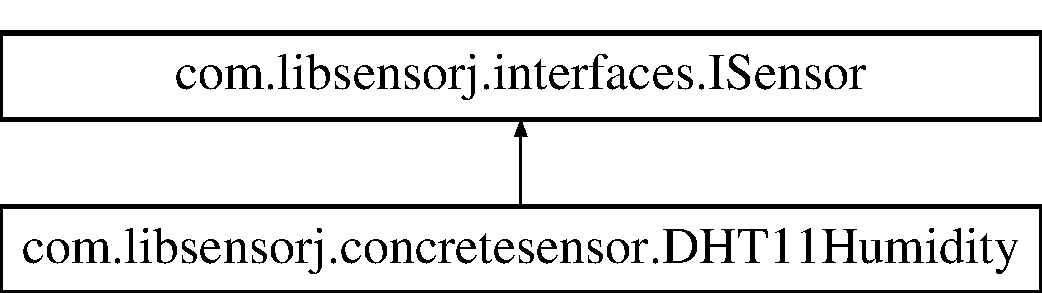
\includegraphics[height=2.000000cm]{classcom_1_1libsensorj_1_1concretesensor_1_1DHT11Humidity}
\end{center}
\end{figure}
\subsection*{Public Member Functions}
\begin{DoxyCompactItemize}
\item 
void \hyperlink{classcom_1_1libsensorj_1_1concretesensor_1_1DHT11Humidity_a2355dc003abad8d519440e9f6871c422}{get\+Instance} ()
\end{DoxyCompactItemize}
\subsection*{Static Private Attributes}
\begin{DoxyCompactItemize}
\item 
static final Logger \hyperlink{classcom_1_1libsensorj_1_1concretesensor_1_1DHT11Humidity_a80655575ba16db014b7a1a797e030eae}{L\+O\+G\+G\+E\+R}
\end{DoxyCompactItemize}


\subsection{Detailed Description}
The Class \hyperlink{classcom_1_1libsensorj_1_1concretesensor_1_1DHT11Humidity}{D\+H\+T11\+Humidity}. 

\subsection{Member Function Documentation}
\hypertarget{classcom_1_1libsensorj_1_1concretesensor_1_1DHT11Humidity_a2355dc003abad8d519440e9f6871c422}{}\index{com\+::libsensorj\+::concretesensor\+::\+D\+H\+T11\+Humidity@{com\+::libsensorj\+::concretesensor\+::\+D\+H\+T11\+Humidity}!get\+Instance@{get\+Instance}}
\index{get\+Instance@{get\+Instance}!com\+::libsensorj\+::concretesensor\+::\+D\+H\+T11\+Humidity@{com\+::libsensorj\+::concretesensor\+::\+D\+H\+T11\+Humidity}}
\subsubsection[{get\+Instance}]{\setlength{\rightskip}{0pt plus 5cm}void com.\+libsensorj.\+concretesensor.\+D\+H\+T11\+Humidity.\+get\+Instance (
\begin{DoxyParamCaption}
{}
\end{DoxyParamCaption}
)}\label{classcom_1_1libsensorj_1_1concretesensor_1_1DHT11Humidity_a2355dc003abad8d519440e9f6871c422}
Gets the single instance of I\+Sensor.

\begin{DoxyReturn}{Returns}
single instance of I\+Sensor 
\end{DoxyReturn}


Implements \hyperlink{interfacecom_1_1libsensorj_1_1interfaces_1_1ISensor_a3c3db93a33adecde81a528651790f75e}{com.\+libsensorj.\+interfaces.\+I\+Sensor}.



\subsection{Member Data Documentation}
\hypertarget{classcom_1_1libsensorj_1_1concretesensor_1_1DHT11Humidity_a80655575ba16db014b7a1a797e030eae}{}\index{com\+::libsensorj\+::concretesensor\+::\+D\+H\+T11\+Humidity@{com\+::libsensorj\+::concretesensor\+::\+D\+H\+T11\+Humidity}!L\+O\+G\+G\+E\+R@{L\+O\+G\+G\+E\+R}}
\index{L\+O\+G\+G\+E\+R@{L\+O\+G\+G\+E\+R}!com\+::libsensorj\+::concretesensor\+::\+D\+H\+T11\+Humidity@{com\+::libsensorj\+::concretesensor\+::\+D\+H\+T11\+Humidity}}
\subsubsection[{L\+O\+G\+G\+E\+R}]{\setlength{\rightskip}{0pt plus 5cm}final Logger com.\+libsensorj.\+concretesensor.\+D\+H\+T11\+Humidity.\+L\+O\+G\+G\+E\+R\hspace{0.3cm}{\ttfamily [static]}, {\ttfamily [private]}}\label{classcom_1_1libsensorj_1_1concretesensor_1_1DHT11Humidity_a80655575ba16db014b7a1a797e030eae}
{\bfseries Initial value\+:}
\begin{DoxyCode}
= LogManager
            .getLogger(DHT11Humidity.class.getName())
\end{DoxyCode}
The Constant L\+O\+G\+G\+E\+R. 

The documentation for this class was generated from the following file\+:\begin{DoxyCompactItemize}
\item 
main/java/com/libsensorj/concretesensor/\hyperlink{DHT11Humidity_8java}{D\+H\+T11\+Humidity.\+java}\end{DoxyCompactItemize}

\hypertarget{classcom_1_1libsensorj_1_1concretesensor_1_1DHT11Temperature}{}\section{com.\+libsensorj.\+concretesensor.\+D\+H\+T11\+Temperature Class Reference}
\label{classcom_1_1libsensorj_1_1concretesensor_1_1DHT11Temperature}\index{com.\+libsensorj.\+concretesensor.\+D\+H\+T11\+Temperature@{com.\+libsensorj.\+concretesensor.\+D\+H\+T11\+Temperature}}
Inheritance diagram for com.\+libsensorj.\+concretesensor.\+D\+H\+T11\+Temperature\+:\begin{figure}[H]
\begin{center}
\leavevmode
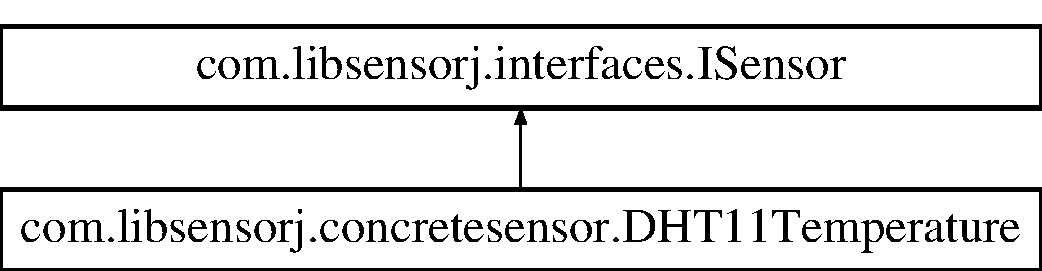
\includegraphics[height=2.000000cm]{classcom_1_1libsensorj_1_1concretesensor_1_1DHT11Temperature}
\end{center}
\end{figure}
\subsection*{Public Member Functions}
\begin{DoxyCompactItemize}
\item 
\hyperlink{classcom_1_1libsensorj_1_1concretesensor_1_1DHT11Temperature_a81324fa18ad12062d493a880f3fbda67}{D\+H\+T11\+Temperature} (int \hyperlink{classcom_1_1libsensorj_1_1concretesensor_1_1DHT11Temperature_a312572f2f0bad8b41d171481ef4e3138}{gpio\+Pin})
\item 
\hyperlink{classcom_1_1libsensorj_1_1concretesensor_1_1DHT11Temperature_a02bbdf30c922adcbde84597bf698ff41}{D\+H\+T11\+Temperature} ()
\item 
void \hyperlink{classcom_1_1libsensorj_1_1concretesensor_1_1DHT11Temperature_a599358623598fb0076dc0a2e07978f0b}{get\+Instance} ()
\item 
synchronized double \hyperlink{classcom_1_1libsensorj_1_1concretesensor_1_1DHT11Temperature_ab0b6a73583d9244271174a3d896f5ed3}{get\+Temperature\+In\+Celsius} ()
\item 
synchronized double \hyperlink{classcom_1_1libsensorj_1_1concretesensor_1_1DHT11Temperature_aa564f9c66609426711cbd0fbfe6837e3}{get\+Temperature\+In\+Fahrenheit} ()
\item 
synchronized double \hyperlink{classcom_1_1libsensorj_1_1concretesensor_1_1DHT11Temperature_a2c1a2bfaaf97612a862079979394ff34}{get\+Temperature\+In\+Kelvin} ()
\end{DoxyCompactItemize}
\subsection*{Private Member Functions}
\begin{DoxyCompactItemize}
\item 
void \hyperlink{classcom_1_1libsensorj_1_1concretesensor_1_1DHT11Temperature_a0ed494577e6a3c68dc737b60f926269d}{check\+For\+Updates} ()
\item 
double \hyperlink{classcom_1_1libsensorj_1_1concretesensor_1_1DHT11Temperature_abb836186013ae429e2cfde981154969b}{get\+Temperature} (Temperature\+Scale from)
\item 
double \hyperlink{classcom_1_1libsensorj_1_1concretesensor_1_1DHT11Temperature_a061220e6439c2014ab81384738c07734}{parse\+Temperature} (String value)
\item 
String \hyperlink{classcom_1_1libsensorj_1_1concretesensor_1_1DHT11Temperature_a2e5125c490d1b7b28a359cf702334fd7}{read\+Values} ()
\end{DoxyCompactItemize}
\subsection*{Private Attributes}
\begin{DoxyCompactItemize}
\item 
String \hyperlink{classcom_1_1libsensorj_1_1concretesensor_1_1DHT11Temperature_af16dd6a4c88dedacb8a4d69d90eff670}{last\+Value}
\item 
long \hyperlink{classcom_1_1libsensorj_1_1concretesensor_1_1DHT11Temperature_a00ec2e3e31bcaf04f497d5c503a84c5e}{last\+Check}
\item 
final int \hyperlink{classcom_1_1libsensorj_1_1concretesensor_1_1DHT11Temperature_a312572f2f0bad8b41d171481ef4e3138}{gpio\+Pin}
\end{DoxyCompactItemize}
\subsection*{Static Private Attributes}
\begin{DoxyCompactItemize}
\item 
static final String \hyperlink{classcom_1_1libsensorj_1_1concretesensor_1_1DHT11Temperature_a123ae6845e0cc1d1ec859cf7cfb78004}{T\+E\+M\+P\+\_\+\+S\+T\+R} = \char`\"{}Temp =\char`\"{}
\item 
static final int \hyperlink{classcom_1_1libsensorj_1_1concretesensor_1_1DHT11Temperature_af8bf5091500d4dcb3b5a0663279359e2}{D\+E\+F\+A\+U\+L\+T\+\_\+\+P\+I\+N} = 4
\item 
static final long \hyperlink{classcom_1_1libsensorj_1_1concretesensor_1_1DHT11Temperature_a7a5b6b6685407c05809a7e4c97358dd4}{L\+A\+S\+T\+\_\+\+C\+H\+E\+C\+K\+\_\+\+D\+I\+F\+F} = 3000
\item 
static final Logger \hyperlink{classcom_1_1libsensorj_1_1concretesensor_1_1DHT11Temperature_a96d485fc09496c1b5a320a30bb3400c9}{L\+O\+G\+G\+E\+R}
\end{DoxyCompactItemize}


\subsection{Detailed Description}
The Class \hyperlink{classcom_1_1libsensorj_1_1concretesensor_1_1DHT11Temperature}{D\+H\+T11\+Temperature}. 

\subsection{Constructor \& Destructor Documentation}
\hypertarget{classcom_1_1libsensorj_1_1concretesensor_1_1DHT11Temperature_a81324fa18ad12062d493a880f3fbda67}{}\index{com\+::libsensorj\+::concretesensor\+::\+D\+H\+T11\+Temperature@{com\+::libsensorj\+::concretesensor\+::\+D\+H\+T11\+Temperature}!D\+H\+T11\+Temperature@{D\+H\+T11\+Temperature}}
\index{D\+H\+T11\+Temperature@{D\+H\+T11\+Temperature}!com\+::libsensorj\+::concretesensor\+::\+D\+H\+T11\+Temperature@{com\+::libsensorj\+::concretesensor\+::\+D\+H\+T11\+Temperature}}
\subsubsection[{D\+H\+T11\+Temperature}]{\setlength{\rightskip}{0pt plus 5cm}com.\+libsensorj.\+concretesensor.\+D\+H\+T11\+Temperature.\+D\+H\+T11\+Temperature (
\begin{DoxyParamCaption}
\item[{int}]{gpio\+Pin}
\end{DoxyParamCaption}
)}\label{classcom_1_1libsensorj_1_1concretesensor_1_1DHT11Temperature_a81324fa18ad12062d493a880f3fbda67}
Instantiates a new D\+Ht11 temperature.


\begin{DoxyParams}{Parameters}
{\em gpio\+Pin} & the gpio pin \\
\hline
\end{DoxyParams}
\hypertarget{classcom_1_1libsensorj_1_1concretesensor_1_1DHT11Temperature_a02bbdf30c922adcbde84597bf698ff41}{}\index{com\+::libsensorj\+::concretesensor\+::\+D\+H\+T11\+Temperature@{com\+::libsensorj\+::concretesensor\+::\+D\+H\+T11\+Temperature}!D\+H\+T11\+Temperature@{D\+H\+T11\+Temperature}}
\index{D\+H\+T11\+Temperature@{D\+H\+T11\+Temperature}!com\+::libsensorj\+::concretesensor\+::\+D\+H\+T11\+Temperature@{com\+::libsensorj\+::concretesensor\+::\+D\+H\+T11\+Temperature}}
\subsubsection[{D\+H\+T11\+Temperature}]{\setlength{\rightskip}{0pt plus 5cm}com.\+libsensorj.\+concretesensor.\+D\+H\+T11\+Temperature.\+D\+H\+T11\+Temperature (
\begin{DoxyParamCaption}
{}
\end{DoxyParamCaption}
)}\label{classcom_1_1libsensorj_1_1concretesensor_1_1DHT11Temperature_a02bbdf30c922adcbde84597bf698ff41}
Instantiates a new D\+Ht11 temperature. 

\subsection{Member Function Documentation}
\hypertarget{classcom_1_1libsensorj_1_1concretesensor_1_1DHT11Temperature_a0ed494577e6a3c68dc737b60f926269d}{}\index{com\+::libsensorj\+::concretesensor\+::\+D\+H\+T11\+Temperature@{com\+::libsensorj\+::concretesensor\+::\+D\+H\+T11\+Temperature}!check\+For\+Updates@{check\+For\+Updates}}
\index{check\+For\+Updates@{check\+For\+Updates}!com\+::libsensorj\+::concretesensor\+::\+D\+H\+T11\+Temperature@{com\+::libsensorj\+::concretesensor\+::\+D\+H\+T11\+Temperature}}
\subsubsection[{check\+For\+Updates}]{\setlength{\rightskip}{0pt plus 5cm}void com.\+libsensorj.\+concretesensor.\+D\+H\+T11\+Temperature.\+check\+For\+Updates (
\begin{DoxyParamCaption}
{}
\end{DoxyParamCaption}
)\hspace{0.3cm}{\ttfamily [private]}}\label{classcom_1_1libsensorj_1_1concretesensor_1_1DHT11Temperature_a0ed494577e6a3c68dc737b60f926269d}
Check for updates. \hypertarget{classcom_1_1libsensorj_1_1concretesensor_1_1DHT11Temperature_a599358623598fb0076dc0a2e07978f0b}{}\index{com\+::libsensorj\+::concretesensor\+::\+D\+H\+T11\+Temperature@{com\+::libsensorj\+::concretesensor\+::\+D\+H\+T11\+Temperature}!get\+Instance@{get\+Instance}}
\index{get\+Instance@{get\+Instance}!com\+::libsensorj\+::concretesensor\+::\+D\+H\+T11\+Temperature@{com\+::libsensorj\+::concretesensor\+::\+D\+H\+T11\+Temperature}}
\subsubsection[{get\+Instance}]{\setlength{\rightskip}{0pt plus 5cm}void com.\+libsensorj.\+concretesensor.\+D\+H\+T11\+Temperature.\+get\+Instance (
\begin{DoxyParamCaption}
{}
\end{DoxyParamCaption}
)}\label{classcom_1_1libsensorj_1_1concretesensor_1_1DHT11Temperature_a599358623598fb0076dc0a2e07978f0b}
Gets the single instance of I\+Sensor.

\begin{DoxyReturn}{Returns}
single instance of I\+Sensor 
\end{DoxyReturn}


Implements \hyperlink{interfacecom_1_1libsensorj_1_1interfaces_1_1ISensor_a3c3db93a33adecde81a528651790f75e}{com.\+libsensorj.\+interfaces.\+I\+Sensor}.

\hypertarget{classcom_1_1libsensorj_1_1concretesensor_1_1DHT11Temperature_abb836186013ae429e2cfde981154969b}{}\index{com\+::libsensorj\+::concretesensor\+::\+D\+H\+T11\+Temperature@{com\+::libsensorj\+::concretesensor\+::\+D\+H\+T11\+Temperature}!get\+Temperature@{get\+Temperature}}
\index{get\+Temperature@{get\+Temperature}!com\+::libsensorj\+::concretesensor\+::\+D\+H\+T11\+Temperature@{com\+::libsensorj\+::concretesensor\+::\+D\+H\+T11\+Temperature}}
\subsubsection[{get\+Temperature}]{\setlength{\rightskip}{0pt plus 5cm}double com.\+libsensorj.\+concretesensor.\+D\+H\+T11\+Temperature.\+get\+Temperature (
\begin{DoxyParamCaption}
\item[{Temperature\+Scale}]{from}
\end{DoxyParamCaption}
)\hspace{0.3cm}{\ttfamily [private]}}\label{classcom_1_1libsensorj_1_1concretesensor_1_1DHT11Temperature_abb836186013ae429e2cfde981154969b}
Gets the temperature.


\begin{DoxyParams}{Parameters}
{\em from} & the from \\
\hline
\end{DoxyParams}
\begin{DoxyReturn}{Returns}
the temperature 
\end{DoxyReturn}
\hypertarget{classcom_1_1libsensorj_1_1concretesensor_1_1DHT11Temperature_ab0b6a73583d9244271174a3d896f5ed3}{}\index{com\+::libsensorj\+::concretesensor\+::\+D\+H\+T11\+Temperature@{com\+::libsensorj\+::concretesensor\+::\+D\+H\+T11\+Temperature}!get\+Temperature\+In\+Celsius@{get\+Temperature\+In\+Celsius}}
\index{get\+Temperature\+In\+Celsius@{get\+Temperature\+In\+Celsius}!com\+::libsensorj\+::concretesensor\+::\+D\+H\+T11\+Temperature@{com\+::libsensorj\+::concretesensor\+::\+D\+H\+T11\+Temperature}}
\subsubsection[{get\+Temperature\+In\+Celsius}]{\setlength{\rightskip}{0pt plus 5cm}synchronized double com.\+libsensorj.\+concretesensor.\+D\+H\+T11\+Temperature.\+get\+Temperature\+In\+Celsius (
\begin{DoxyParamCaption}
{}
\end{DoxyParamCaption}
)}\label{classcom_1_1libsensorj_1_1concretesensor_1_1DHT11Temperature_ab0b6a73583d9244271174a3d896f5ed3}
Gets the temperature in celsius.

\begin{DoxyReturn}{Returns}
the temperature in celsius 
\end{DoxyReturn}
\hypertarget{classcom_1_1libsensorj_1_1concretesensor_1_1DHT11Temperature_aa564f9c66609426711cbd0fbfe6837e3}{}\index{com\+::libsensorj\+::concretesensor\+::\+D\+H\+T11\+Temperature@{com\+::libsensorj\+::concretesensor\+::\+D\+H\+T11\+Temperature}!get\+Temperature\+In\+Fahrenheit@{get\+Temperature\+In\+Fahrenheit}}
\index{get\+Temperature\+In\+Fahrenheit@{get\+Temperature\+In\+Fahrenheit}!com\+::libsensorj\+::concretesensor\+::\+D\+H\+T11\+Temperature@{com\+::libsensorj\+::concretesensor\+::\+D\+H\+T11\+Temperature}}
\subsubsection[{get\+Temperature\+In\+Fahrenheit}]{\setlength{\rightskip}{0pt plus 5cm}synchronized double com.\+libsensorj.\+concretesensor.\+D\+H\+T11\+Temperature.\+get\+Temperature\+In\+Fahrenheit (
\begin{DoxyParamCaption}
{}
\end{DoxyParamCaption}
)}\label{classcom_1_1libsensorj_1_1concretesensor_1_1DHT11Temperature_aa564f9c66609426711cbd0fbfe6837e3}
Gets the temperature in fahrenheit.

\begin{DoxyReturn}{Returns}
the temperature in fahrenheit 
\end{DoxyReturn}
\hypertarget{classcom_1_1libsensorj_1_1concretesensor_1_1DHT11Temperature_a2c1a2bfaaf97612a862079979394ff34}{}\index{com\+::libsensorj\+::concretesensor\+::\+D\+H\+T11\+Temperature@{com\+::libsensorj\+::concretesensor\+::\+D\+H\+T11\+Temperature}!get\+Temperature\+In\+Kelvin@{get\+Temperature\+In\+Kelvin}}
\index{get\+Temperature\+In\+Kelvin@{get\+Temperature\+In\+Kelvin}!com\+::libsensorj\+::concretesensor\+::\+D\+H\+T11\+Temperature@{com\+::libsensorj\+::concretesensor\+::\+D\+H\+T11\+Temperature}}
\subsubsection[{get\+Temperature\+In\+Kelvin}]{\setlength{\rightskip}{0pt plus 5cm}synchronized double com.\+libsensorj.\+concretesensor.\+D\+H\+T11\+Temperature.\+get\+Temperature\+In\+Kelvin (
\begin{DoxyParamCaption}
{}
\end{DoxyParamCaption}
)}\label{classcom_1_1libsensorj_1_1concretesensor_1_1DHT11Temperature_a2c1a2bfaaf97612a862079979394ff34}
Gets the temperature in kelvin.

\begin{DoxyReturn}{Returns}
the temperature in kelvin 
\end{DoxyReturn}
\hypertarget{classcom_1_1libsensorj_1_1concretesensor_1_1DHT11Temperature_a061220e6439c2014ab81384738c07734}{}\index{com\+::libsensorj\+::concretesensor\+::\+D\+H\+T11\+Temperature@{com\+::libsensorj\+::concretesensor\+::\+D\+H\+T11\+Temperature}!parse\+Temperature@{parse\+Temperature}}
\index{parse\+Temperature@{parse\+Temperature}!com\+::libsensorj\+::concretesensor\+::\+D\+H\+T11\+Temperature@{com\+::libsensorj\+::concretesensor\+::\+D\+H\+T11\+Temperature}}
\subsubsection[{parse\+Temperature}]{\setlength{\rightskip}{0pt plus 5cm}double com.\+libsensorj.\+concretesensor.\+D\+H\+T11\+Temperature.\+parse\+Temperature (
\begin{DoxyParamCaption}
\item[{String}]{value}
\end{DoxyParamCaption}
)\hspace{0.3cm}{\ttfamily [private]}}\label{classcom_1_1libsensorj_1_1concretesensor_1_1DHT11Temperature_a061220e6439c2014ab81384738c07734}
Parses the temperature.


\begin{DoxyParams}{Parameters}
{\em value} & the value \\
\hline
\end{DoxyParams}
\begin{DoxyReturn}{Returns}
the double 
\end{DoxyReturn}
\hypertarget{classcom_1_1libsensorj_1_1concretesensor_1_1DHT11Temperature_a2e5125c490d1b7b28a359cf702334fd7}{}\index{com\+::libsensorj\+::concretesensor\+::\+D\+H\+T11\+Temperature@{com\+::libsensorj\+::concretesensor\+::\+D\+H\+T11\+Temperature}!read\+Values@{read\+Values}}
\index{read\+Values@{read\+Values}!com\+::libsensorj\+::concretesensor\+::\+D\+H\+T11\+Temperature@{com\+::libsensorj\+::concretesensor\+::\+D\+H\+T11\+Temperature}}
\subsubsection[{read\+Values}]{\setlength{\rightskip}{0pt plus 5cm}String com.\+libsensorj.\+concretesensor.\+D\+H\+T11\+Temperature.\+read\+Values (
\begin{DoxyParamCaption}
{}
\end{DoxyParamCaption}
)\hspace{0.3cm}{\ttfamily [private]}}\label{classcom_1_1libsensorj_1_1concretesensor_1_1DHT11Temperature_a2e5125c490d1b7b28a359cf702334fd7}
Read values.

\begin{DoxyReturn}{Returns}
the value readed as a string 
\end{DoxyReturn}


\subsection{Member Data Documentation}
\hypertarget{classcom_1_1libsensorj_1_1concretesensor_1_1DHT11Temperature_af8bf5091500d4dcb3b5a0663279359e2}{}\index{com\+::libsensorj\+::concretesensor\+::\+D\+H\+T11\+Temperature@{com\+::libsensorj\+::concretesensor\+::\+D\+H\+T11\+Temperature}!D\+E\+F\+A\+U\+L\+T\+\_\+\+P\+I\+N@{D\+E\+F\+A\+U\+L\+T\+\_\+\+P\+I\+N}}
\index{D\+E\+F\+A\+U\+L\+T\+\_\+\+P\+I\+N@{D\+E\+F\+A\+U\+L\+T\+\_\+\+P\+I\+N}!com\+::libsensorj\+::concretesensor\+::\+D\+H\+T11\+Temperature@{com\+::libsensorj\+::concretesensor\+::\+D\+H\+T11\+Temperature}}
\subsubsection[{D\+E\+F\+A\+U\+L\+T\+\_\+\+P\+I\+N}]{\setlength{\rightskip}{0pt plus 5cm}final int com.\+libsensorj.\+concretesensor.\+D\+H\+T11\+Temperature.\+D\+E\+F\+A\+U\+L\+T\+\_\+\+P\+I\+N = 4\hspace{0.3cm}{\ttfamily [static]}, {\ttfamily [private]}}\label{classcom_1_1libsensorj_1_1concretesensor_1_1DHT11Temperature_af8bf5091500d4dcb3b5a0663279359e2}
The Constant D\+E\+F\+A\+U\+L\+T\+\_\+\+P\+I\+N. \hypertarget{classcom_1_1libsensorj_1_1concretesensor_1_1DHT11Temperature_a312572f2f0bad8b41d171481ef4e3138}{}\index{com\+::libsensorj\+::concretesensor\+::\+D\+H\+T11\+Temperature@{com\+::libsensorj\+::concretesensor\+::\+D\+H\+T11\+Temperature}!gpio\+Pin@{gpio\+Pin}}
\index{gpio\+Pin@{gpio\+Pin}!com\+::libsensorj\+::concretesensor\+::\+D\+H\+T11\+Temperature@{com\+::libsensorj\+::concretesensor\+::\+D\+H\+T11\+Temperature}}
\subsubsection[{gpio\+Pin}]{\setlength{\rightskip}{0pt plus 5cm}final int com.\+libsensorj.\+concretesensor.\+D\+H\+T11\+Temperature.\+gpio\+Pin\hspace{0.3cm}{\ttfamily [private]}}\label{classcom_1_1libsensorj_1_1concretesensor_1_1DHT11Temperature_a312572f2f0bad8b41d171481ef4e3138}
The gpio pin. \hypertarget{classcom_1_1libsensorj_1_1concretesensor_1_1DHT11Temperature_a7a5b6b6685407c05809a7e4c97358dd4}{}\index{com\+::libsensorj\+::concretesensor\+::\+D\+H\+T11\+Temperature@{com\+::libsensorj\+::concretesensor\+::\+D\+H\+T11\+Temperature}!L\+A\+S\+T\+\_\+\+C\+H\+E\+C\+K\+\_\+\+D\+I\+F\+F@{L\+A\+S\+T\+\_\+\+C\+H\+E\+C\+K\+\_\+\+D\+I\+F\+F}}
\index{L\+A\+S\+T\+\_\+\+C\+H\+E\+C\+K\+\_\+\+D\+I\+F\+F@{L\+A\+S\+T\+\_\+\+C\+H\+E\+C\+K\+\_\+\+D\+I\+F\+F}!com\+::libsensorj\+::concretesensor\+::\+D\+H\+T11\+Temperature@{com\+::libsensorj\+::concretesensor\+::\+D\+H\+T11\+Temperature}}
\subsubsection[{L\+A\+S\+T\+\_\+\+C\+H\+E\+C\+K\+\_\+\+D\+I\+F\+F}]{\setlength{\rightskip}{0pt plus 5cm}final long com.\+libsensorj.\+concretesensor.\+D\+H\+T11\+Temperature.\+L\+A\+S\+T\+\_\+\+C\+H\+E\+C\+K\+\_\+\+D\+I\+F\+F = 3000\hspace{0.3cm}{\ttfamily [static]}, {\ttfamily [private]}}\label{classcom_1_1libsensorj_1_1concretesensor_1_1DHT11Temperature_a7a5b6b6685407c05809a7e4c97358dd4}
The Constant L\+A\+S\+T\+\_\+\+C\+H\+E\+C\+K\+\_\+\+D\+I\+F\+F. \hypertarget{classcom_1_1libsensorj_1_1concretesensor_1_1DHT11Temperature_a00ec2e3e31bcaf04f497d5c503a84c5e}{}\index{com\+::libsensorj\+::concretesensor\+::\+D\+H\+T11\+Temperature@{com\+::libsensorj\+::concretesensor\+::\+D\+H\+T11\+Temperature}!last\+Check@{last\+Check}}
\index{last\+Check@{last\+Check}!com\+::libsensorj\+::concretesensor\+::\+D\+H\+T11\+Temperature@{com\+::libsensorj\+::concretesensor\+::\+D\+H\+T11\+Temperature}}
\subsubsection[{last\+Check}]{\setlength{\rightskip}{0pt plus 5cm}long com.\+libsensorj.\+concretesensor.\+D\+H\+T11\+Temperature.\+last\+Check\hspace{0.3cm}{\ttfamily [private]}}\label{classcom_1_1libsensorj_1_1concretesensor_1_1DHT11Temperature_a00ec2e3e31bcaf04f497d5c503a84c5e}
The last check. \hypertarget{classcom_1_1libsensorj_1_1concretesensor_1_1DHT11Temperature_af16dd6a4c88dedacb8a4d69d90eff670}{}\index{com\+::libsensorj\+::concretesensor\+::\+D\+H\+T11\+Temperature@{com\+::libsensorj\+::concretesensor\+::\+D\+H\+T11\+Temperature}!last\+Value@{last\+Value}}
\index{last\+Value@{last\+Value}!com\+::libsensorj\+::concretesensor\+::\+D\+H\+T11\+Temperature@{com\+::libsensorj\+::concretesensor\+::\+D\+H\+T11\+Temperature}}
\subsubsection[{last\+Value}]{\setlength{\rightskip}{0pt plus 5cm}String com.\+libsensorj.\+concretesensor.\+D\+H\+T11\+Temperature.\+last\+Value\hspace{0.3cm}{\ttfamily [private]}}\label{classcom_1_1libsensorj_1_1concretesensor_1_1DHT11Temperature_af16dd6a4c88dedacb8a4d69d90eff670}
The last value. \hypertarget{classcom_1_1libsensorj_1_1concretesensor_1_1DHT11Temperature_a96d485fc09496c1b5a320a30bb3400c9}{}\index{com\+::libsensorj\+::concretesensor\+::\+D\+H\+T11\+Temperature@{com\+::libsensorj\+::concretesensor\+::\+D\+H\+T11\+Temperature}!L\+O\+G\+G\+E\+R@{L\+O\+G\+G\+E\+R}}
\index{L\+O\+G\+G\+E\+R@{L\+O\+G\+G\+E\+R}!com\+::libsensorj\+::concretesensor\+::\+D\+H\+T11\+Temperature@{com\+::libsensorj\+::concretesensor\+::\+D\+H\+T11\+Temperature}}
\subsubsection[{L\+O\+G\+G\+E\+R}]{\setlength{\rightskip}{0pt plus 5cm}final Logger com.\+libsensorj.\+concretesensor.\+D\+H\+T11\+Temperature.\+L\+O\+G\+G\+E\+R\hspace{0.3cm}{\ttfamily [static]}, {\ttfamily [private]}}\label{classcom_1_1libsensorj_1_1concretesensor_1_1DHT11Temperature_a96d485fc09496c1b5a320a30bb3400c9}
{\bfseries Initial value\+:}
\begin{DoxyCode}
= LogManager
            .getLogger(\hyperlink{classcom_1_1libsensorj_1_1concretesensor_1_1DHT11Temperature_a02bbdf30c922adcbde84597bf698ff41}{DHT11Temperature}.class.getName())
\end{DoxyCode}
The Constant L\+O\+G\+G\+E\+R. \hypertarget{classcom_1_1libsensorj_1_1concretesensor_1_1DHT11Temperature_a123ae6845e0cc1d1ec859cf7cfb78004}{}\index{com\+::libsensorj\+::concretesensor\+::\+D\+H\+T11\+Temperature@{com\+::libsensorj\+::concretesensor\+::\+D\+H\+T11\+Temperature}!T\+E\+M\+P\+\_\+\+S\+T\+R@{T\+E\+M\+P\+\_\+\+S\+T\+R}}
\index{T\+E\+M\+P\+\_\+\+S\+T\+R@{T\+E\+M\+P\+\_\+\+S\+T\+R}!com\+::libsensorj\+::concretesensor\+::\+D\+H\+T11\+Temperature@{com\+::libsensorj\+::concretesensor\+::\+D\+H\+T11\+Temperature}}
\subsubsection[{T\+E\+M\+P\+\_\+\+S\+T\+R}]{\setlength{\rightskip}{0pt plus 5cm}final String com.\+libsensorj.\+concretesensor.\+D\+H\+T11\+Temperature.\+T\+E\+M\+P\+\_\+\+S\+T\+R = \char`\"{}Temp =\char`\"{}\hspace{0.3cm}{\ttfamily [static]}, {\ttfamily [private]}}\label{classcom_1_1libsensorj_1_1concretesensor_1_1DHT11Temperature_a123ae6845e0cc1d1ec859cf7cfb78004}
The Constant T\+E\+M\+P\+\_\+\+S\+T\+R. 

The documentation for this class was generated from the following file\+:\begin{DoxyCompactItemize}
\item 
main/java/com/libsensorj/concretesensor/\hyperlink{DHT11Temperature_8java}{D\+H\+T11\+Temperature.\+java}\end{DoxyCompactItemize}

\hypertarget{classcom_1_1libsensorj_1_1examples_1_1DHT11TemperatureExample}{}\section{com.\+libsensorj.\+examples.\+D\+H\+T11\+Temperature\+Example Class Reference}
\label{classcom_1_1libsensorj_1_1examples_1_1DHT11TemperatureExample}\index{com.\+libsensorj.\+examples.\+D\+H\+T11\+Temperature\+Example@{com.\+libsensorj.\+examples.\+D\+H\+T11\+Temperature\+Example}}
\subsection*{Static Public Member Functions}
\begin{DoxyCompactItemize}
\item 
static void \hyperlink{classcom_1_1libsensorj_1_1examples_1_1DHT11TemperatureExample_a436567d5cd7d4e55dbed6438386af490}{main} (String\mbox{[}$\,$\mbox{]} args)
\end{DoxyCompactItemize}
\subsection*{Static Private Attributes}
\begin{DoxyCompactItemize}
\item 
static \hyperlink{interfacecom_1_1libsensorj_1_1interfaces_1_1ISensor}{I\+Sensor} \hyperlink{classcom_1_1libsensorj_1_1examples_1_1DHT11TemperatureExample_ae5b24da8a75b04b9f313d9b4aaa2f058}{dht11}
\end{DoxyCompactItemize}


\subsection{Member Function Documentation}
\hypertarget{classcom_1_1libsensorj_1_1examples_1_1DHT11TemperatureExample_a436567d5cd7d4e55dbed6438386af490}{}\index{com\+::libsensorj\+::examples\+::\+D\+H\+T11\+Temperature\+Example@{com\+::libsensorj\+::examples\+::\+D\+H\+T11\+Temperature\+Example}!main@{main}}
\index{main@{main}!com\+::libsensorj\+::examples\+::\+D\+H\+T11\+Temperature\+Example@{com\+::libsensorj\+::examples\+::\+D\+H\+T11\+Temperature\+Example}}
\subsubsection[{main}]{\setlength{\rightskip}{0pt plus 5cm}static void com.\+libsensorj.\+examples.\+D\+H\+T11\+Temperature\+Example.\+main (
\begin{DoxyParamCaption}
\item[{String\mbox{[}$\,$\mbox{]}}]{args}
\end{DoxyParamCaption}
)\hspace{0.3cm}{\ttfamily [static]}}\label{classcom_1_1libsensorj_1_1examples_1_1DHT11TemperatureExample_a436567d5cd7d4e55dbed6438386af490}


\subsection{Member Data Documentation}
\hypertarget{classcom_1_1libsensorj_1_1examples_1_1DHT11TemperatureExample_ae5b24da8a75b04b9f313d9b4aaa2f058}{}\index{com\+::libsensorj\+::examples\+::\+D\+H\+T11\+Temperature\+Example@{com\+::libsensorj\+::examples\+::\+D\+H\+T11\+Temperature\+Example}!dht11@{dht11}}
\index{dht11@{dht11}!com\+::libsensorj\+::examples\+::\+D\+H\+T11\+Temperature\+Example@{com\+::libsensorj\+::examples\+::\+D\+H\+T11\+Temperature\+Example}}
\subsubsection[{dht11}]{\setlength{\rightskip}{0pt plus 5cm}{\bf I\+Sensor} com.\+libsensorj.\+examples.\+D\+H\+T11\+Temperature\+Example.\+dht11\hspace{0.3cm}{\ttfamily [static]}, {\ttfamily [private]}}\label{classcom_1_1libsensorj_1_1examples_1_1DHT11TemperatureExample_ae5b24da8a75b04b9f313d9b4aaa2f058}


The documentation for this class was generated from the following file\+:\begin{DoxyCompactItemize}
\item 
main/java/com/libsensorj/examples/\hyperlink{DHT11TemperatureExample_8java}{D\+H\+T11\+Temperature\+Example.\+java}\end{DoxyCompactItemize}

\hypertarget{classcom_1_1pi4j_1_1examples_1_1Example}{}\section{com.\+pi4j.\+examples.\+Example Class Reference}
\label{classcom_1_1pi4j_1_1examples_1_1Example}\index{com.\+pi4j.\+examples.\+Example@{com.\+pi4j.\+examples.\+Example}}
\subsection*{Static Public Member Functions}
\begin{DoxyCompactItemize}
\item 
static void \hyperlink{classcom_1_1pi4j_1_1examples_1_1Example_ab706c9d868d8965a7b8b88abb6db15fa}{main} (String\mbox{[}$\,$\mbox{]} args)  throws Interrupted\+Exception 
\item 
static void \hyperlink{classcom_1_1pi4j_1_1examples_1_1Example_ab14dd3a0a5a91192e576cecf0aa9ad5c}{read} ()
\item 
static String \hyperlink{classcom_1_1pi4j_1_1examples_1_1Example_a55c7417721387ecdaf6c27c413cb395e}{bytes\+To\+Binary} (byte\mbox{[}$\,$\mbox{]} bytes)
\item 
static String \hyperlink{classcom_1_1pi4j_1_1examples_1_1Example_ae71c0b716fdae032b20b52666a6668ce}{bytes\+To\+Hex} (byte\mbox{[}$\,$\mbox{]} bytes)
\end{DoxyCompactItemize}
\subsection*{Static Public Attributes}
\begin{DoxyCompactItemize}
\item 
static final byte \hyperlink{classcom_1_1pi4j_1_1examples_1_1Example_a9fe242ff65eed0f1f399b8e9a0e50ccd}{I\+N\+I\+T\+\_\+\+C\+M\+D} = (byte) 0x\+D0
\item 
static final byte \hyperlink{classcom_1_1pi4j_1_1examples_1_1Example_a467713cca966503adb0e98f963ca894e}{S\+P\+I\+\_\+\+C\+H\+A\+N\+N\+E\+L} = 0x0
\end{DoxyCompactItemize}
\subsection*{Static Private Attributes}
\begin{DoxyCompactItemize}
\item 
static final String \hyperlink{classcom_1_1pi4j_1_1examples_1_1Example_aebff74f082fb0684ef3c7cd361ea0480}{T\+R\+A\+C\+E\+D\+\_\+\+L\+I\+N\+E} = \char`\"{}-\/-\/-\/-\/-\/-\/-\/-\/-\/-\/-\/-\/-\/-\/-\/-\/-\/-\/-\/-\/-\/-\/-\/-\/-\/-\/-\/-\/-\/-\/-\/-\/-\/-\/-\/-\/-\/-\/-\/-\/-\/-\/-\/-\/-\/-\/-\/\char`\"{}
\item 
static final Logger \hyperlink{classcom_1_1pi4j_1_1examples_1_1Example_ae8e218a8535d844b1b928cfc835a30ba}{L\+O\+G\+G\+E\+R}
\end{DoxyCompactItemize}


\subsection{Member Function Documentation}
\hypertarget{classcom_1_1pi4j_1_1examples_1_1Example_a55c7417721387ecdaf6c27c413cb395e}{}\index{com\+::pi4j\+::examples\+::\+Example@{com\+::pi4j\+::examples\+::\+Example}!bytes\+To\+Binary@{bytes\+To\+Binary}}
\index{bytes\+To\+Binary@{bytes\+To\+Binary}!com\+::pi4j\+::examples\+::\+Example@{com\+::pi4j\+::examples\+::\+Example}}
\subsubsection[{bytes\+To\+Binary}]{\setlength{\rightskip}{0pt plus 5cm}static String com.\+pi4j.\+examples.\+Example.\+bytes\+To\+Binary (
\begin{DoxyParamCaption}
\item[{byte\mbox{[}$\,$\mbox{]}}]{bytes}
\end{DoxyParamCaption}
)\hspace{0.3cm}{\ttfamily [static]}}\label{classcom_1_1pi4j_1_1examples_1_1Example_a55c7417721387ecdaf6c27c413cb395e}
\hypertarget{classcom_1_1pi4j_1_1examples_1_1Example_ae71c0b716fdae032b20b52666a6668ce}{}\index{com\+::pi4j\+::examples\+::\+Example@{com\+::pi4j\+::examples\+::\+Example}!bytes\+To\+Hex@{bytes\+To\+Hex}}
\index{bytes\+To\+Hex@{bytes\+To\+Hex}!com\+::pi4j\+::examples\+::\+Example@{com\+::pi4j\+::examples\+::\+Example}}
\subsubsection[{bytes\+To\+Hex}]{\setlength{\rightskip}{0pt plus 5cm}static String com.\+pi4j.\+examples.\+Example.\+bytes\+To\+Hex (
\begin{DoxyParamCaption}
\item[{byte\mbox{[}$\,$\mbox{]}}]{bytes}
\end{DoxyParamCaption}
)\hspace{0.3cm}{\ttfamily [static]}}\label{classcom_1_1pi4j_1_1examples_1_1Example_ae71c0b716fdae032b20b52666a6668ce}
\hypertarget{classcom_1_1pi4j_1_1examples_1_1Example_ab706c9d868d8965a7b8b88abb6db15fa}{}\index{com\+::pi4j\+::examples\+::\+Example@{com\+::pi4j\+::examples\+::\+Example}!main@{main}}
\index{main@{main}!com\+::pi4j\+::examples\+::\+Example@{com\+::pi4j\+::examples\+::\+Example}}
\subsubsection[{main}]{\setlength{\rightskip}{0pt plus 5cm}static void com.\+pi4j.\+examples.\+Example.\+main (
\begin{DoxyParamCaption}
\item[{String\mbox{[}$\,$\mbox{]}}]{args}
\end{DoxyParamCaption}
) throws Interrupted\+Exception\hspace{0.3cm}{\ttfamily [static]}}\label{classcom_1_1pi4j_1_1examples_1_1Example_ab706c9d868d8965a7b8b88abb6db15fa}
\hypertarget{classcom_1_1pi4j_1_1examples_1_1Example_ab14dd3a0a5a91192e576cecf0aa9ad5c}{}\index{com\+::pi4j\+::examples\+::\+Example@{com\+::pi4j\+::examples\+::\+Example}!read@{read}}
\index{read@{read}!com\+::pi4j\+::examples\+::\+Example@{com\+::pi4j\+::examples\+::\+Example}}
\subsubsection[{read}]{\setlength{\rightskip}{0pt plus 5cm}static void com.\+pi4j.\+examples.\+Example.\+read (
\begin{DoxyParamCaption}
{}
\end{DoxyParamCaption}
)\hspace{0.3cm}{\ttfamily [static]}}\label{classcom_1_1pi4j_1_1examples_1_1Example_ab14dd3a0a5a91192e576cecf0aa9ad5c}


\subsection{Member Data Documentation}
\hypertarget{classcom_1_1pi4j_1_1examples_1_1Example_a9fe242ff65eed0f1f399b8e9a0e50ccd}{}\index{com\+::pi4j\+::examples\+::\+Example@{com\+::pi4j\+::examples\+::\+Example}!I\+N\+I\+T\+\_\+\+C\+M\+D@{I\+N\+I\+T\+\_\+\+C\+M\+D}}
\index{I\+N\+I\+T\+\_\+\+C\+M\+D@{I\+N\+I\+T\+\_\+\+C\+M\+D}!com\+::pi4j\+::examples\+::\+Example@{com\+::pi4j\+::examples\+::\+Example}}
\subsubsection[{I\+N\+I\+T\+\_\+\+C\+M\+D}]{\setlength{\rightskip}{0pt plus 5cm}final byte com.\+pi4j.\+examples.\+Example.\+I\+N\+I\+T\+\_\+\+C\+M\+D = (byte) 0x\+D0\hspace{0.3cm}{\ttfamily [static]}}\label{classcom_1_1pi4j_1_1examples_1_1Example_a9fe242ff65eed0f1f399b8e9a0e50ccd}
\hypertarget{classcom_1_1pi4j_1_1examples_1_1Example_ae8e218a8535d844b1b928cfc835a30ba}{}\index{com\+::pi4j\+::examples\+::\+Example@{com\+::pi4j\+::examples\+::\+Example}!L\+O\+G\+G\+E\+R@{L\+O\+G\+G\+E\+R}}
\index{L\+O\+G\+G\+E\+R@{L\+O\+G\+G\+E\+R}!com\+::pi4j\+::examples\+::\+Example@{com\+::pi4j\+::examples\+::\+Example}}
\subsubsection[{L\+O\+G\+G\+E\+R}]{\setlength{\rightskip}{0pt plus 5cm}final Logger com.\+pi4j.\+examples.\+Example.\+L\+O\+G\+G\+E\+R\hspace{0.3cm}{\ttfamily [static]}, {\ttfamily [private]}}\label{classcom_1_1pi4j_1_1examples_1_1Example_ae8e218a8535d844b1b928cfc835a30ba}
{\bfseries Initial value\+:}
\begin{DoxyCode}
= LogManager.getLogger(Example.class
            .getName())
\end{DoxyCode}
\hypertarget{classcom_1_1pi4j_1_1examples_1_1Example_a467713cca966503adb0e98f963ca894e}{}\index{com\+::pi4j\+::examples\+::\+Example@{com\+::pi4j\+::examples\+::\+Example}!S\+P\+I\+\_\+\+C\+H\+A\+N\+N\+E\+L@{S\+P\+I\+\_\+\+C\+H\+A\+N\+N\+E\+L}}
\index{S\+P\+I\+\_\+\+C\+H\+A\+N\+N\+E\+L@{S\+P\+I\+\_\+\+C\+H\+A\+N\+N\+E\+L}!com\+::pi4j\+::examples\+::\+Example@{com\+::pi4j\+::examples\+::\+Example}}
\subsubsection[{S\+P\+I\+\_\+\+C\+H\+A\+N\+N\+E\+L}]{\setlength{\rightskip}{0pt plus 5cm}final byte com.\+pi4j.\+examples.\+Example.\+S\+P\+I\+\_\+\+C\+H\+A\+N\+N\+E\+L = 0x0\hspace{0.3cm}{\ttfamily [static]}}\label{classcom_1_1pi4j_1_1examples_1_1Example_a467713cca966503adb0e98f963ca894e}
\hypertarget{classcom_1_1pi4j_1_1examples_1_1Example_aebff74f082fb0684ef3c7cd361ea0480}{}\index{com\+::pi4j\+::examples\+::\+Example@{com\+::pi4j\+::examples\+::\+Example}!T\+R\+A\+C\+E\+D\+\_\+\+L\+I\+N\+E@{T\+R\+A\+C\+E\+D\+\_\+\+L\+I\+N\+E}}
\index{T\+R\+A\+C\+E\+D\+\_\+\+L\+I\+N\+E@{T\+R\+A\+C\+E\+D\+\_\+\+L\+I\+N\+E}!com\+::pi4j\+::examples\+::\+Example@{com\+::pi4j\+::examples\+::\+Example}}
\subsubsection[{T\+R\+A\+C\+E\+D\+\_\+\+L\+I\+N\+E}]{\setlength{\rightskip}{0pt plus 5cm}final String com.\+pi4j.\+examples.\+Example.\+T\+R\+A\+C\+E\+D\+\_\+\+L\+I\+N\+E = \char`\"{}-\/-\/-\/-\/-\/-\/-\/-\/-\/-\/-\/-\/-\/-\/-\/-\/-\/-\/-\/-\/-\/-\/-\/-\/-\/-\/-\/-\/-\/-\/-\/-\/-\/-\/-\/-\/-\/-\/-\/-\/-\/-\/-\/-\/-\/-\/-\/\char`\"{}\hspace{0.3cm}{\ttfamily [static]}, {\ttfamily [private]}}\label{classcom_1_1pi4j_1_1examples_1_1Example_aebff74f082fb0684ef3c7cd361ea0480}


The documentation for this class was generated from the following file\+:\begin{DoxyCompactItemize}
\item 
main/java/com/pi4j/examples/\hyperlink{Example_8java}{Example.\+java}\end{DoxyCompactItemize}

\hypertarget{classcom_1_1pi4j_1_1examples_1_1FrequencyGpioExample}{}\section{com.\+pi4j.\+examples.\+Frequency\+Gpio\+Example Class Reference}
\label{classcom_1_1pi4j_1_1examples_1_1FrequencyGpioExample}\index{com.\+pi4j.\+examples.\+Frequency\+Gpio\+Example@{com.\+pi4j.\+examples.\+Frequency\+Gpio\+Example}}
\subsection*{Static Public Member Functions}
\begin{DoxyCompactItemize}
\item 
static void \hyperlink{classcom_1_1pi4j_1_1examples_1_1FrequencyGpioExample_a7aa7e22b034f94ba794e9ed2005305c4}{main} (String\mbox{[}$\,$\mbox{]} args)
\end{DoxyCompactItemize}
\subsection*{Static Private Attributes}
\begin{DoxyCompactItemize}
\item 
static final Logger \hyperlink{classcom_1_1pi4j_1_1examples_1_1FrequencyGpioExample_a3d0645e2d0163919ac0caa7af24da6b1}{L\+O\+G\+G\+E\+R}
\end{DoxyCompactItemize}


\subsection{Detailed Description}
This example code provides a continuous G\+P\+I\+O pin state changes on the Raspberry Pi to allow measurement of frequency.

\begin{DoxyAuthor}{Author}
Robert Savage 
\end{DoxyAuthor}


\subsection{Member Function Documentation}
\hypertarget{classcom_1_1pi4j_1_1examples_1_1FrequencyGpioExample_a7aa7e22b034f94ba794e9ed2005305c4}{}\index{com\+::pi4j\+::examples\+::\+Frequency\+Gpio\+Example@{com\+::pi4j\+::examples\+::\+Frequency\+Gpio\+Example}!main@{main}}
\index{main@{main}!com\+::pi4j\+::examples\+::\+Frequency\+Gpio\+Example@{com\+::pi4j\+::examples\+::\+Frequency\+Gpio\+Example}}
\subsubsection[{main}]{\setlength{\rightskip}{0pt plus 5cm}static void com.\+pi4j.\+examples.\+Frequency\+Gpio\+Example.\+main (
\begin{DoxyParamCaption}
\item[{String\mbox{[}$\,$\mbox{]}}]{args}
\end{DoxyParamCaption}
)\hspace{0.3cm}{\ttfamily [static]}}\label{classcom_1_1pi4j_1_1examples_1_1FrequencyGpioExample_a7aa7e22b034f94ba794e9ed2005305c4}


\subsection{Member Data Documentation}
\hypertarget{classcom_1_1pi4j_1_1examples_1_1FrequencyGpioExample_a3d0645e2d0163919ac0caa7af24da6b1}{}\index{com\+::pi4j\+::examples\+::\+Frequency\+Gpio\+Example@{com\+::pi4j\+::examples\+::\+Frequency\+Gpio\+Example}!L\+O\+G\+G\+E\+R@{L\+O\+G\+G\+E\+R}}
\index{L\+O\+G\+G\+E\+R@{L\+O\+G\+G\+E\+R}!com\+::pi4j\+::examples\+::\+Frequency\+Gpio\+Example@{com\+::pi4j\+::examples\+::\+Frequency\+Gpio\+Example}}
\subsubsection[{L\+O\+G\+G\+E\+R}]{\setlength{\rightskip}{0pt plus 5cm}final Logger com.\+pi4j.\+examples.\+Frequency\+Gpio\+Example.\+L\+O\+G\+G\+E\+R\hspace{0.3cm}{\ttfamily [static]}, {\ttfamily [private]}}\label{classcom_1_1pi4j_1_1examples_1_1FrequencyGpioExample_a3d0645e2d0163919ac0caa7af24da6b1}
{\bfseries Initial value\+:}
\begin{DoxyCode}
= LogManager
            .getLogger(FrequencyGpioExample.class.getName())
\end{DoxyCode}


The documentation for this class was generated from the following file\+:\begin{DoxyCompactItemize}
\item 
main/java/com/pi4j/examples/\hyperlink{FrequencyGpioExample_8java}{Frequency\+Gpio\+Example.\+java}\end{DoxyCompactItemize}

\hypertarget{classcom_1_1pi4j_1_1examples_1_1UsageGpioExample_1_1GpioUsageExampleListener}{}\section{com.\+pi4j.\+examples.\+Usage\+Gpio\+Example.\+Gpio\+Usage\+Example\+Listener Class Reference}
\label{classcom_1_1pi4j_1_1examples_1_1UsageGpioExample_1_1GpioUsageExampleListener}\index{com.\+pi4j.\+examples.\+Usage\+Gpio\+Example.\+Gpio\+Usage\+Example\+Listener@{com.\+pi4j.\+examples.\+Usage\+Gpio\+Example.\+Gpio\+Usage\+Example\+Listener}}
Inheritance diagram for com.\+pi4j.\+examples.\+Usage\+Gpio\+Example.\+Gpio\+Usage\+Example\+Listener\+:\begin{figure}[H]
\begin{center}
\leavevmode
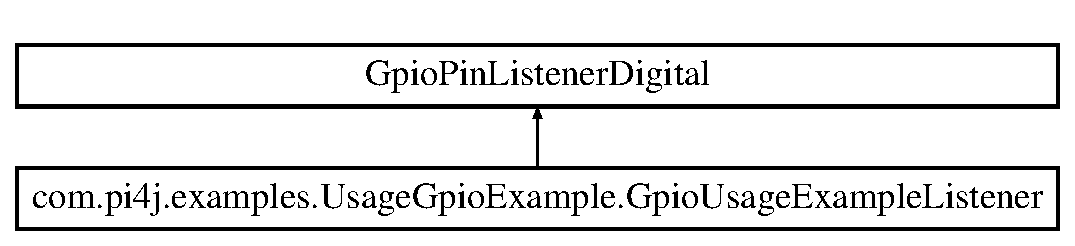
\includegraphics[height=2.000000cm]{classcom_1_1pi4j_1_1examples_1_1UsageGpioExample_1_1GpioUsageExampleListener}
\end{center}
\end{figure}
\subsection*{Public Member Functions}
\begin{DoxyCompactItemize}
\item 
void \hyperlink{classcom_1_1pi4j_1_1examples_1_1UsageGpioExample_1_1GpioUsageExampleListener_a5cae5b046b260a1a2f8090366270d821}{handle\+Gpio\+Pin\+Digital\+State\+Change\+Event} (Gpio\+Pin\+Digital\+State\+Change\+Event event)
\end{DoxyCompactItemize}


\subsection{Member Function Documentation}
\hypertarget{classcom_1_1pi4j_1_1examples_1_1UsageGpioExample_1_1GpioUsageExampleListener_a5cae5b046b260a1a2f8090366270d821}{}\index{com\+::pi4j\+::examples\+::\+Usage\+Gpio\+Example\+::\+Gpio\+Usage\+Example\+Listener@{com\+::pi4j\+::examples\+::\+Usage\+Gpio\+Example\+::\+Gpio\+Usage\+Example\+Listener}!handle\+Gpio\+Pin\+Digital\+State\+Change\+Event@{handle\+Gpio\+Pin\+Digital\+State\+Change\+Event}}
\index{handle\+Gpio\+Pin\+Digital\+State\+Change\+Event@{handle\+Gpio\+Pin\+Digital\+State\+Change\+Event}!com\+::pi4j\+::examples\+::\+Usage\+Gpio\+Example\+::\+Gpio\+Usage\+Example\+Listener@{com\+::pi4j\+::examples\+::\+Usage\+Gpio\+Example\+::\+Gpio\+Usage\+Example\+Listener}}
\subsubsection[{handle\+Gpio\+Pin\+Digital\+State\+Change\+Event}]{\setlength{\rightskip}{0pt plus 5cm}void com.\+pi4j.\+examples.\+Usage\+Gpio\+Example.\+Gpio\+Usage\+Example\+Listener.\+handle\+Gpio\+Pin\+Digital\+State\+Change\+Event (
\begin{DoxyParamCaption}
\item[{Gpio\+Pin\+Digital\+State\+Change\+Event}]{event}
\end{DoxyParamCaption}
)}\label{classcom_1_1pi4j_1_1examples_1_1UsageGpioExample_1_1GpioUsageExampleListener_a5cae5b046b260a1a2f8090366270d821}


The documentation for this class was generated from the following file\+:\begin{DoxyCompactItemize}
\item 
main/java/com/pi4j/examples/\hyperlink{UsageGpioExample_8java}{Usage\+Gpio\+Example.\+java}\end{DoxyCompactItemize}

\hypertarget{classcom_1_1libsensorj_1_1concreteevent_1_1HumidityEvent}{}\section{com.\+libsensorj.\+concreteevent.\+Humidity\+Event Class Reference}
\label{classcom_1_1libsensorj_1_1concreteevent_1_1HumidityEvent}\index{com.\+libsensorj.\+concreteevent.\+Humidity\+Event@{com.\+libsensorj.\+concreteevent.\+Humidity\+Event}}
Inheritance diagram for com.\+libsensorj.\+concreteevent.\+Humidity\+Event\+:\begin{figure}[H]
\begin{center}
\leavevmode
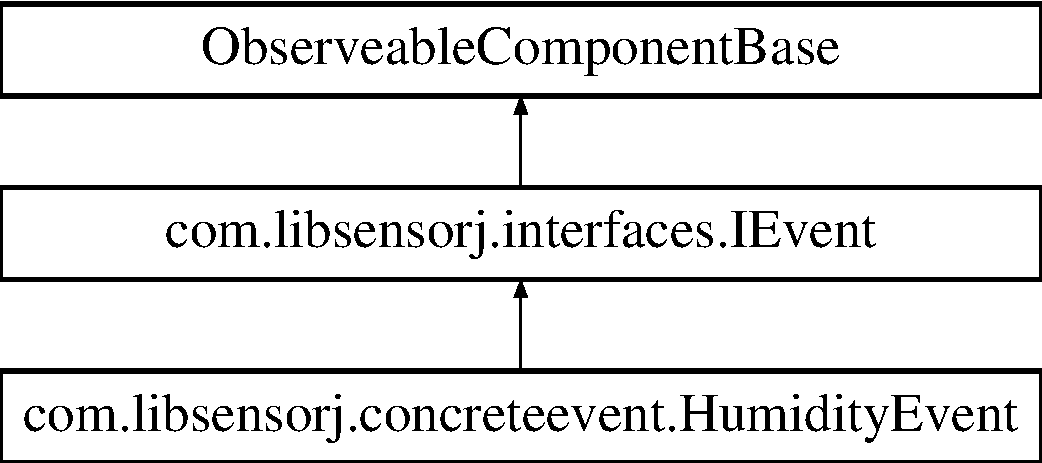
\includegraphics[height=2.000000cm]{classcom_1_1libsensorj_1_1concreteevent_1_1HumidityEvent}
\end{center}
\end{figure}
\subsection*{Public Member Functions}
\begin{DoxyCompactItemize}
\item 
void \hyperlink{classcom_1_1libsensorj_1_1concreteevent_1_1HumidityEvent_a4ea7f94d2402aeafca55dc1fb2950d00}{attach} (\hyperlink{classcom_1_1libsensorj_1_1model_1_1Observer}{Observer} obsever)
\item 
void \hyperlink{classcom_1_1libsensorj_1_1concreteevent_1_1HumidityEvent_a577a1f99a7993ccd8019fb46c1668c9b}{detach} (\hyperlink{classcom_1_1libsensorj_1_1model_1_1Observer}{Observer} obsever)
\item 
void \hyperlink{classcom_1_1libsensorj_1_1concreteevent_1_1HumidityEvent_ad3d8c57f1934c115f0c9374394d9a601}{trigger} ()
\end{DoxyCompactItemize}


\subsection{Member Function Documentation}
\hypertarget{classcom_1_1libsensorj_1_1concreteevent_1_1HumidityEvent_a4ea7f94d2402aeafca55dc1fb2950d00}{}\index{com\+::libsensorj\+::concreteevent\+::\+Humidity\+Event@{com\+::libsensorj\+::concreteevent\+::\+Humidity\+Event}!attach@{attach}}
\index{attach@{attach}!com\+::libsensorj\+::concreteevent\+::\+Humidity\+Event@{com\+::libsensorj\+::concreteevent\+::\+Humidity\+Event}}
\subsubsection[{attach}]{\setlength{\rightskip}{0pt plus 5cm}void com.\+libsensorj.\+concreteevent.\+Humidity\+Event.\+attach (
\begin{DoxyParamCaption}
\item[{{\bf Observer}}]{obsever}
\end{DoxyParamCaption}
)}\label{classcom_1_1libsensorj_1_1concreteevent_1_1HumidityEvent_a4ea7f94d2402aeafca55dc1fb2950d00}


Implements \hyperlink{interfacecom_1_1libsensorj_1_1interfaces_1_1IEvent_af5af4301ccb6670452419d68baddf372}{com.\+libsensorj.\+interfaces.\+I\+Event}.

\hypertarget{classcom_1_1libsensorj_1_1concreteevent_1_1HumidityEvent_a577a1f99a7993ccd8019fb46c1668c9b}{}\index{com\+::libsensorj\+::concreteevent\+::\+Humidity\+Event@{com\+::libsensorj\+::concreteevent\+::\+Humidity\+Event}!detach@{detach}}
\index{detach@{detach}!com\+::libsensorj\+::concreteevent\+::\+Humidity\+Event@{com\+::libsensorj\+::concreteevent\+::\+Humidity\+Event}}
\subsubsection[{detach}]{\setlength{\rightskip}{0pt plus 5cm}void com.\+libsensorj.\+concreteevent.\+Humidity\+Event.\+detach (
\begin{DoxyParamCaption}
\item[{{\bf Observer}}]{obsever}
\end{DoxyParamCaption}
)}\label{classcom_1_1libsensorj_1_1concreteevent_1_1HumidityEvent_a577a1f99a7993ccd8019fb46c1668c9b}


Implements \hyperlink{interfacecom_1_1libsensorj_1_1interfaces_1_1IEvent_a974b07df97fda9f3be8e4afcd46470b2}{com.\+libsensorj.\+interfaces.\+I\+Event}.

\hypertarget{classcom_1_1libsensorj_1_1concreteevent_1_1HumidityEvent_ad3d8c57f1934c115f0c9374394d9a601}{}\index{com\+::libsensorj\+::concreteevent\+::\+Humidity\+Event@{com\+::libsensorj\+::concreteevent\+::\+Humidity\+Event}!trigger@{trigger}}
\index{trigger@{trigger}!com\+::libsensorj\+::concreteevent\+::\+Humidity\+Event@{com\+::libsensorj\+::concreteevent\+::\+Humidity\+Event}}
\subsubsection[{trigger}]{\setlength{\rightskip}{0pt plus 5cm}void com.\+libsensorj.\+concreteevent.\+Humidity\+Event.\+trigger (
\begin{DoxyParamCaption}
{}
\end{DoxyParamCaption}
)}\label{classcom_1_1libsensorj_1_1concreteevent_1_1HumidityEvent_ad3d8c57f1934c115f0c9374394d9a601}


Implements \hyperlink{interfacecom_1_1libsensorj_1_1interfaces_1_1IEvent_a861dea0956f77dd82f95e0110b8043b2}{com.\+libsensorj.\+interfaces.\+I\+Event}.



The documentation for this class was generated from the following file\+:\begin{DoxyCompactItemize}
\item 
main/java/com/libsensorj/concreteevent/\hyperlink{HumidityEvent_8java}{Humidity\+Event.\+java}\end{DoxyCompactItemize}

\hypertarget{classcom_1_1libsensorj_1_1concretefactory_1_1HumiditySensorFactory}{}\section{com.\+libsensorj.\+concretefactory.\+Humidity\+Sensor\+Factory Class Reference}
\label{classcom_1_1libsensorj_1_1concretefactory_1_1HumiditySensorFactory}\index{com.\+libsensorj.\+concretefactory.\+Humidity\+Sensor\+Factory@{com.\+libsensorj.\+concretefactory.\+Humidity\+Sensor\+Factory}}
Inheritance diagram for com.\+libsensorj.\+concretefactory.\+Humidity\+Sensor\+Factory\+:\begin{figure}[H]
\begin{center}
\leavevmode
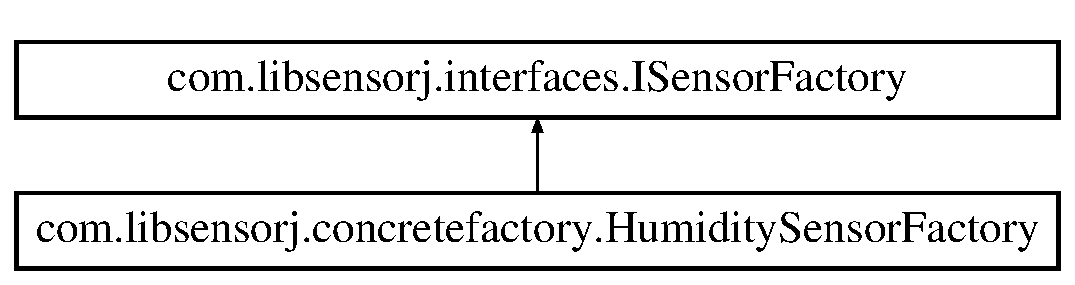
\includegraphics[height=2.000000cm]{classcom_1_1libsensorj_1_1concretefactory_1_1HumiditySensorFactory}
\end{center}
\end{figure}
\subsection*{Public Member Functions}
\begin{DoxyCompactItemize}
\item 
\hyperlink{interfacecom_1_1libsensorj_1_1interfaces_1_1ISensor}{I\+Sensor} \hyperlink{classcom_1_1libsensorj_1_1concretefactory_1_1HumiditySensorFactory_aec6f80bd08e69d69ea6187067d11d28c}{create\+Sensor} ()
\item 
\hyperlink{classcom_1_1libsensorj_1_1interfaces_1_1IEvent}{I\+Event} \hyperlink{classcom_1_1libsensorj_1_1concretefactory_1_1HumiditySensorFactory_a43835bfa4c60faf39dfe64f67322b9e4}{create\+Event} ()
\end{DoxyCompactItemize}


\subsection{Detailed Description}
A factory for creating Humidity\+Sensor objects. 

\subsection{Member Function Documentation}
\hypertarget{classcom_1_1libsensorj_1_1concretefactory_1_1HumiditySensorFactory_a43835bfa4c60faf39dfe64f67322b9e4}{}\index{com\+::libsensorj\+::concretefactory\+::\+Humidity\+Sensor\+Factory@{com\+::libsensorj\+::concretefactory\+::\+Humidity\+Sensor\+Factory}!create\+Event@{create\+Event}}
\index{create\+Event@{create\+Event}!com\+::libsensorj\+::concretefactory\+::\+Humidity\+Sensor\+Factory@{com\+::libsensorj\+::concretefactory\+::\+Humidity\+Sensor\+Factory}}
\subsubsection[{create\+Event}]{\setlength{\rightskip}{0pt plus 5cm}{\bf I\+Event} com.\+libsensorj.\+concretefactory.\+Humidity\+Sensor\+Factory.\+create\+Event (
\begin{DoxyParamCaption}
{}
\end{DoxyParamCaption}
)}\label{classcom_1_1libsensorj_1_1concretefactory_1_1HumiditySensorFactory_a43835bfa4c60faf39dfe64f67322b9e4}
Creates a new I\+Event object.

\begin{DoxyReturn}{Returns}
the I\+Event 
\end{DoxyReturn}


Implements \hyperlink{interfacecom_1_1libsensorj_1_1interfaces_1_1ISensorFactory_a2b074d01287a4e64677097255ba9e768}{com.\+libsensorj.\+interfaces.\+I\+Sensor\+Factory}.

\hypertarget{classcom_1_1libsensorj_1_1concretefactory_1_1HumiditySensorFactory_aec6f80bd08e69d69ea6187067d11d28c}{}\index{com\+::libsensorj\+::concretefactory\+::\+Humidity\+Sensor\+Factory@{com\+::libsensorj\+::concretefactory\+::\+Humidity\+Sensor\+Factory}!create\+Sensor@{create\+Sensor}}
\index{create\+Sensor@{create\+Sensor}!com\+::libsensorj\+::concretefactory\+::\+Humidity\+Sensor\+Factory@{com\+::libsensorj\+::concretefactory\+::\+Humidity\+Sensor\+Factory}}
\subsubsection[{create\+Sensor}]{\setlength{\rightskip}{0pt plus 5cm}{\bf I\+Sensor} com.\+libsensorj.\+concretefactory.\+Humidity\+Sensor\+Factory.\+create\+Sensor (
\begin{DoxyParamCaption}
{}
\end{DoxyParamCaption}
)}\label{classcom_1_1libsensorj_1_1concretefactory_1_1HumiditySensorFactory_aec6f80bd08e69d69ea6187067d11d28c}
Creates a new I\+Sensor object.

\begin{DoxyReturn}{Returns}
the I\+Sensor 
\end{DoxyReturn}


Implements \hyperlink{interfacecom_1_1libsensorj_1_1interfaces_1_1ISensorFactory_ac14c6d566c37c6a79c6db1e85634f25d}{com.\+libsensorj.\+interfaces.\+I\+Sensor\+Factory}.



The documentation for this class was generated from the following file\+:\begin{DoxyCompactItemize}
\item 
main/java/com/libsensorj/concretefactory/\hyperlink{HumiditySensorFactory_8java}{Humidity\+Sensor\+Factory.\+java}\end{DoxyCompactItemize}

\hypertarget{classcom_1_1pi4j_1_1examples_1_1I2CWiiMotionPlusExample}{}\section{com.\+pi4j.\+examples.\+I2\+C\+Wii\+Motion\+Plus\+Example Class Reference}
\label{classcom_1_1pi4j_1_1examples_1_1I2CWiiMotionPlusExample}\index{com.\+pi4j.\+examples.\+I2\+C\+Wii\+Motion\+Plus\+Example@{com.\+pi4j.\+examples.\+I2\+C\+Wii\+Motion\+Plus\+Example}}
\subsection*{Classes}
\begin{DoxyCompactItemize}
\item 
class \hyperlink{classcom_1_1pi4j_1_1examples_1_1I2CWiiMotionPlusExample_1_1ThreeAxis}{Three\+Axis}
\item 
class \hyperlink{classcom_1_1pi4j_1_1examples_1_1I2CWiiMotionPlusExample_1_1WiiMotionPlus}{Wii\+Motion\+Plus}
\end{DoxyCompactItemize}
\subsection*{Static Public Member Functions}
\begin{DoxyCompactItemize}
\item 
static void \hyperlink{classcom_1_1pi4j_1_1examples_1_1I2CWiiMotionPlusExample_ab70f795c9aaeef444dbd9536494e97bf}{main} (String\mbox{[}$\,$\mbox{]} args)  throws Exception 
\item 
static void \hyperlink{classcom_1_1pi4j_1_1examples_1_1I2CWiiMotionPlusExample_a69aaf1e91321cf49920fe5c6d62ebd86}{make\+Backup} (String filename)
\item 
static String \hyperlink{classcom_1_1pi4j_1_1examples_1_1I2CWiiMotionPlusExample_ad4e3fbbe78e17178df5c60b748f270ea}{format\+Int} (int i)
\item 
static String \hyperlink{classcom_1_1pi4j_1_1examples_1_1I2CWiiMotionPlusExample_a6bb2cf35eceb2902df176f7cd9447943}{format\+Long} (long i)
\end{DoxyCompactItemize}
\subsection*{Static Private Attributes}
\begin{DoxyCompactItemize}
\item 
static final String \hyperlink{classcom_1_1pi4j_1_1examples_1_1I2CWiiMotionPlusExample_a79cb6b5d2e13a7d078a04935985de532}{L\+O\+G\+\_\+\+F\+I\+L\+E} = \char`\"{}log.\+txt\char`\"{}
\item 
static final Logger \hyperlink{classcom_1_1pi4j_1_1examples_1_1I2CWiiMotionPlusExample_a8cc3c8ff3d397904bd9e6dd8a82644d7}{L\+O\+G\+G\+E\+R}
\item 
static final String \hyperlink{classcom_1_1pi4j_1_1examples_1_1I2CWiiMotionPlusExample_a6ec0a220e417a66f10e90138b00f93ab}{E\+M\+P\+T\+Y\+\_\+\+S\+T\+R\+I\+N\+G} = \char`\"{} \char`\"{}
\end{DoxyCompactItemize}


\subsection{Member Function Documentation}
\hypertarget{classcom_1_1pi4j_1_1examples_1_1I2CWiiMotionPlusExample_ad4e3fbbe78e17178df5c60b748f270ea}{}\index{com\+::pi4j\+::examples\+::\+I2\+C\+Wii\+Motion\+Plus\+Example@{com\+::pi4j\+::examples\+::\+I2\+C\+Wii\+Motion\+Plus\+Example}!format\+Int@{format\+Int}}
\index{format\+Int@{format\+Int}!com\+::pi4j\+::examples\+::\+I2\+C\+Wii\+Motion\+Plus\+Example@{com\+::pi4j\+::examples\+::\+I2\+C\+Wii\+Motion\+Plus\+Example}}
\subsubsection[{format\+Int}]{\setlength{\rightskip}{0pt plus 5cm}static String com.\+pi4j.\+examples.\+I2\+C\+Wii\+Motion\+Plus\+Example.\+format\+Int (
\begin{DoxyParamCaption}
\item[{int}]{i}
\end{DoxyParamCaption}
)\hspace{0.3cm}{\ttfamily [static]}}\label{classcom_1_1pi4j_1_1examples_1_1I2CWiiMotionPlusExample_ad4e3fbbe78e17178df5c60b748f270ea}
\hypertarget{classcom_1_1pi4j_1_1examples_1_1I2CWiiMotionPlusExample_a6bb2cf35eceb2902df176f7cd9447943}{}\index{com\+::pi4j\+::examples\+::\+I2\+C\+Wii\+Motion\+Plus\+Example@{com\+::pi4j\+::examples\+::\+I2\+C\+Wii\+Motion\+Plus\+Example}!format\+Long@{format\+Long}}
\index{format\+Long@{format\+Long}!com\+::pi4j\+::examples\+::\+I2\+C\+Wii\+Motion\+Plus\+Example@{com\+::pi4j\+::examples\+::\+I2\+C\+Wii\+Motion\+Plus\+Example}}
\subsubsection[{format\+Long}]{\setlength{\rightskip}{0pt plus 5cm}static String com.\+pi4j.\+examples.\+I2\+C\+Wii\+Motion\+Plus\+Example.\+format\+Long (
\begin{DoxyParamCaption}
\item[{long}]{i}
\end{DoxyParamCaption}
)\hspace{0.3cm}{\ttfamily [static]}}\label{classcom_1_1pi4j_1_1examples_1_1I2CWiiMotionPlusExample_a6bb2cf35eceb2902df176f7cd9447943}
\hypertarget{classcom_1_1pi4j_1_1examples_1_1I2CWiiMotionPlusExample_ab70f795c9aaeef444dbd9536494e97bf}{}\index{com\+::pi4j\+::examples\+::\+I2\+C\+Wii\+Motion\+Plus\+Example@{com\+::pi4j\+::examples\+::\+I2\+C\+Wii\+Motion\+Plus\+Example}!main@{main}}
\index{main@{main}!com\+::pi4j\+::examples\+::\+I2\+C\+Wii\+Motion\+Plus\+Example@{com\+::pi4j\+::examples\+::\+I2\+C\+Wii\+Motion\+Plus\+Example}}
\subsubsection[{main}]{\setlength{\rightskip}{0pt plus 5cm}static void com.\+pi4j.\+examples.\+I2\+C\+Wii\+Motion\+Plus\+Example.\+main (
\begin{DoxyParamCaption}
\item[{String\mbox{[}$\,$\mbox{]}}]{args}
\end{DoxyParamCaption}
) throws Exception\hspace{0.3cm}{\ttfamily [static]}}\label{classcom_1_1pi4j_1_1examples_1_1I2CWiiMotionPlusExample_ab70f795c9aaeef444dbd9536494e97bf}

\begin{DoxyParams}{Parameters}
{\em args} & \\
\hline
\end{DoxyParams}
\hypertarget{classcom_1_1pi4j_1_1examples_1_1I2CWiiMotionPlusExample_a69aaf1e91321cf49920fe5c6d62ebd86}{}\index{com\+::pi4j\+::examples\+::\+I2\+C\+Wii\+Motion\+Plus\+Example@{com\+::pi4j\+::examples\+::\+I2\+C\+Wii\+Motion\+Plus\+Example}!make\+Backup@{make\+Backup}}
\index{make\+Backup@{make\+Backup}!com\+::pi4j\+::examples\+::\+I2\+C\+Wii\+Motion\+Plus\+Example@{com\+::pi4j\+::examples\+::\+I2\+C\+Wii\+Motion\+Plus\+Example}}
\subsubsection[{make\+Backup}]{\setlength{\rightskip}{0pt plus 5cm}static void com.\+pi4j.\+examples.\+I2\+C\+Wii\+Motion\+Plus\+Example.\+make\+Backup (
\begin{DoxyParamCaption}
\item[{String}]{filename}
\end{DoxyParamCaption}
)\hspace{0.3cm}{\ttfamily [static]}}\label{classcom_1_1pi4j_1_1examples_1_1I2CWiiMotionPlusExample_a69aaf1e91321cf49920fe5c6d62ebd86}


\subsection{Member Data Documentation}
\hypertarget{classcom_1_1pi4j_1_1examples_1_1I2CWiiMotionPlusExample_a6ec0a220e417a66f10e90138b00f93ab}{}\index{com\+::pi4j\+::examples\+::\+I2\+C\+Wii\+Motion\+Plus\+Example@{com\+::pi4j\+::examples\+::\+I2\+C\+Wii\+Motion\+Plus\+Example}!E\+M\+P\+T\+Y\+\_\+\+S\+T\+R\+I\+N\+G@{E\+M\+P\+T\+Y\+\_\+\+S\+T\+R\+I\+N\+G}}
\index{E\+M\+P\+T\+Y\+\_\+\+S\+T\+R\+I\+N\+G@{E\+M\+P\+T\+Y\+\_\+\+S\+T\+R\+I\+N\+G}!com\+::pi4j\+::examples\+::\+I2\+C\+Wii\+Motion\+Plus\+Example@{com\+::pi4j\+::examples\+::\+I2\+C\+Wii\+Motion\+Plus\+Example}}
\subsubsection[{E\+M\+P\+T\+Y\+\_\+\+S\+T\+R\+I\+N\+G}]{\setlength{\rightskip}{0pt plus 5cm}final String com.\+pi4j.\+examples.\+I2\+C\+Wii\+Motion\+Plus\+Example.\+E\+M\+P\+T\+Y\+\_\+\+S\+T\+R\+I\+N\+G = \char`\"{} \char`\"{}\hspace{0.3cm}{\ttfamily [static]}, {\ttfamily [private]}}\label{classcom_1_1pi4j_1_1examples_1_1I2CWiiMotionPlusExample_a6ec0a220e417a66f10e90138b00f93ab}
\hypertarget{classcom_1_1pi4j_1_1examples_1_1I2CWiiMotionPlusExample_a79cb6b5d2e13a7d078a04935985de532}{}\index{com\+::pi4j\+::examples\+::\+I2\+C\+Wii\+Motion\+Plus\+Example@{com\+::pi4j\+::examples\+::\+I2\+C\+Wii\+Motion\+Plus\+Example}!L\+O\+G\+\_\+\+F\+I\+L\+E@{L\+O\+G\+\_\+\+F\+I\+L\+E}}
\index{L\+O\+G\+\_\+\+F\+I\+L\+E@{L\+O\+G\+\_\+\+F\+I\+L\+E}!com\+::pi4j\+::examples\+::\+I2\+C\+Wii\+Motion\+Plus\+Example@{com\+::pi4j\+::examples\+::\+I2\+C\+Wii\+Motion\+Plus\+Example}}
\subsubsection[{L\+O\+G\+\_\+\+F\+I\+L\+E}]{\setlength{\rightskip}{0pt plus 5cm}final String com.\+pi4j.\+examples.\+I2\+C\+Wii\+Motion\+Plus\+Example.\+L\+O\+G\+\_\+\+F\+I\+L\+E = \char`\"{}log.\+txt\char`\"{}\hspace{0.3cm}{\ttfamily [static]}, {\ttfamily [private]}}\label{classcom_1_1pi4j_1_1examples_1_1I2CWiiMotionPlusExample_a79cb6b5d2e13a7d078a04935985de532}
\hypertarget{classcom_1_1pi4j_1_1examples_1_1I2CWiiMotionPlusExample_a8cc3c8ff3d397904bd9e6dd8a82644d7}{}\index{com\+::pi4j\+::examples\+::\+I2\+C\+Wii\+Motion\+Plus\+Example@{com\+::pi4j\+::examples\+::\+I2\+C\+Wii\+Motion\+Plus\+Example}!L\+O\+G\+G\+E\+R@{L\+O\+G\+G\+E\+R}}
\index{L\+O\+G\+G\+E\+R@{L\+O\+G\+G\+E\+R}!com\+::pi4j\+::examples\+::\+I2\+C\+Wii\+Motion\+Plus\+Example@{com\+::pi4j\+::examples\+::\+I2\+C\+Wii\+Motion\+Plus\+Example}}
\subsubsection[{L\+O\+G\+G\+E\+R}]{\setlength{\rightskip}{0pt plus 5cm}final Logger com.\+pi4j.\+examples.\+I2\+C\+Wii\+Motion\+Plus\+Example.\+L\+O\+G\+G\+E\+R\hspace{0.3cm}{\ttfamily [static]}, {\ttfamily [private]}}\label{classcom_1_1pi4j_1_1examples_1_1I2CWiiMotionPlusExample_a8cc3c8ff3d397904bd9e6dd8a82644d7}
{\bfseries Initial value\+:}
\begin{DoxyCode}
= LogManager
            .getLogger(I2CWiiMotionPlusExample.class.getName())
\end{DoxyCode}


The documentation for this class was generated from the following file\+:\begin{DoxyCompactItemize}
\item 
main/java/com/pi4j/examples/\hyperlink{I2CWiiMotionPlusExample_8java}{I2\+C\+Wii\+Motion\+Plus\+Example.\+java}\end{DoxyCompactItemize}

\hypertarget{interfacecom_1_1libsensorj_1_1interfaces_1_1IEvent}{}\section{com.\+libsensorj.\+interfaces.\+I\+Event Interface Reference}
\label{interfacecom_1_1libsensorj_1_1interfaces_1_1IEvent}\index{com.\+libsensorj.\+interfaces.\+I\+Event@{com.\+libsensorj.\+interfaces.\+I\+Event}}
Inheritance diagram for com.\+libsensorj.\+interfaces.\+I\+Event\+:\begin{figure}[H]
\begin{center}
\leavevmode
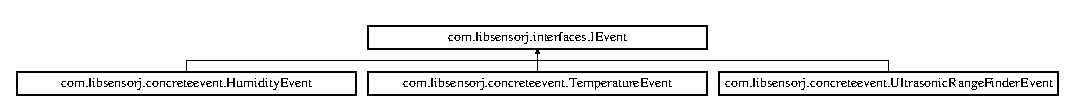
\includegraphics[height=1.063628cm]{interfacecom_1_1libsensorj_1_1interfaces_1_1IEvent}
\end{center}
\end{figure}
\subsection*{Public Member Functions}
\begin{DoxyCompactItemize}
\item 
void \hyperlink{interfacecom_1_1libsensorj_1_1interfaces_1_1IEvent_af5af4301ccb6670452419d68baddf372}{attach} (\hyperlink{classcom_1_1libsensorj_1_1model_1_1Observer}{Observer} obsever)
\item 
void \hyperlink{interfacecom_1_1libsensorj_1_1interfaces_1_1IEvent_a974b07df97fda9f3be8e4afcd46470b2}{detach} (\hyperlink{classcom_1_1libsensorj_1_1model_1_1Observer}{Observer} obsever)
\item 
void \hyperlink{interfacecom_1_1libsensorj_1_1interfaces_1_1IEvent_a861dea0956f77dd82f95e0110b8043b2}{trigger} ()
\end{DoxyCompactItemize}


\subsection{Member Function Documentation}
\hypertarget{interfacecom_1_1libsensorj_1_1interfaces_1_1IEvent_af5af4301ccb6670452419d68baddf372}{}\index{com\+::libsensorj\+::interfaces\+::\+I\+Event@{com\+::libsensorj\+::interfaces\+::\+I\+Event}!attach@{attach}}
\index{attach@{attach}!com\+::libsensorj\+::interfaces\+::\+I\+Event@{com\+::libsensorj\+::interfaces\+::\+I\+Event}}
\subsubsection[{attach}]{\setlength{\rightskip}{0pt plus 5cm}void com.\+libsensorj.\+interfaces.\+I\+Event.\+attach (
\begin{DoxyParamCaption}
\item[{{\bf Observer}}]{obsever}
\end{DoxyParamCaption}
)}\label{interfacecom_1_1libsensorj_1_1interfaces_1_1IEvent_af5af4301ccb6670452419d68baddf372}


Implemented in \hyperlink{classcom_1_1libsensorj_1_1concreteevent_1_1HumidityEvent_a4ea7f94d2402aeafca55dc1fb2950d00}{com.\+libsensorj.\+concreteevent.\+Humidity\+Event}, \hyperlink{classcom_1_1libsensorj_1_1concreteevent_1_1TemperatureEvent_ad3499315aef403dfde60cf7d9a42c8cf}{com.\+libsensorj.\+concreteevent.\+Temperature\+Event}, and \hyperlink{classcom_1_1libsensorj_1_1concreteevent_1_1UltrasonicRangeFinderEvent_a0b32d3efeb55247269b4f43e4e34fe8e}{com.\+libsensorj.\+concreteevent.\+Ultrasonic\+Range\+Finder\+Event}.

\hypertarget{interfacecom_1_1libsensorj_1_1interfaces_1_1IEvent_a974b07df97fda9f3be8e4afcd46470b2}{}\index{com\+::libsensorj\+::interfaces\+::\+I\+Event@{com\+::libsensorj\+::interfaces\+::\+I\+Event}!detach@{detach}}
\index{detach@{detach}!com\+::libsensorj\+::interfaces\+::\+I\+Event@{com\+::libsensorj\+::interfaces\+::\+I\+Event}}
\subsubsection[{detach}]{\setlength{\rightskip}{0pt plus 5cm}void com.\+libsensorj.\+interfaces.\+I\+Event.\+detach (
\begin{DoxyParamCaption}
\item[{{\bf Observer}}]{obsever}
\end{DoxyParamCaption}
)}\label{interfacecom_1_1libsensorj_1_1interfaces_1_1IEvent_a974b07df97fda9f3be8e4afcd46470b2}


Implemented in \hyperlink{classcom_1_1libsensorj_1_1concreteevent_1_1HumidityEvent_a577a1f99a7993ccd8019fb46c1668c9b}{com.\+libsensorj.\+concreteevent.\+Humidity\+Event}, \hyperlink{classcom_1_1libsensorj_1_1concreteevent_1_1TemperatureEvent_a7332f144af23c349f39dd714de9c07b9}{com.\+libsensorj.\+concreteevent.\+Temperature\+Event}, and \hyperlink{classcom_1_1libsensorj_1_1concreteevent_1_1UltrasonicRangeFinderEvent_ab0647f65e87ff07f61b3e4fe7e1daa19}{com.\+libsensorj.\+concreteevent.\+Ultrasonic\+Range\+Finder\+Event}.

\hypertarget{interfacecom_1_1libsensorj_1_1interfaces_1_1IEvent_a861dea0956f77dd82f95e0110b8043b2}{}\index{com\+::libsensorj\+::interfaces\+::\+I\+Event@{com\+::libsensorj\+::interfaces\+::\+I\+Event}!trigger@{trigger}}
\index{trigger@{trigger}!com\+::libsensorj\+::interfaces\+::\+I\+Event@{com\+::libsensorj\+::interfaces\+::\+I\+Event}}
\subsubsection[{trigger}]{\setlength{\rightskip}{0pt plus 5cm}void com.\+libsensorj.\+interfaces.\+I\+Event.\+trigger (
\begin{DoxyParamCaption}
{}
\end{DoxyParamCaption}
)}\label{interfacecom_1_1libsensorj_1_1interfaces_1_1IEvent_a861dea0956f77dd82f95e0110b8043b2}


Implemented in \hyperlink{classcom_1_1libsensorj_1_1concreteevent_1_1HumidityEvent_ad3d8c57f1934c115f0c9374394d9a601}{com.\+libsensorj.\+concreteevent.\+Humidity\+Event}, \hyperlink{classcom_1_1libsensorj_1_1concreteevent_1_1TemperatureEvent_ac0fe5a9964739808ece4fc9f2562dca5}{com.\+libsensorj.\+concreteevent.\+Temperature\+Event}, and \hyperlink{classcom_1_1libsensorj_1_1concreteevent_1_1UltrasonicRangeFinderEvent_a4d1ba316d1d324c4fb6e321e4c7a7b6e}{com.\+libsensorj.\+concreteevent.\+Ultrasonic\+Range\+Finder\+Event}.



The documentation for this interface was generated from the following file\+:\begin{DoxyCompactItemize}
\item 
main/java/com/libsensorj/interfaces/\hyperlink{IEvent_8java}{I\+Event.\+java}\end{DoxyCompactItemize}

\hypertarget{interfacecom_1_1libsensorj_1_1interfaces_1_1ISensor}{}\section{com.\+libsensorj.\+interfaces.\+I\+Sensor Interface Reference}
\label{interfacecom_1_1libsensorj_1_1interfaces_1_1ISensor}\index{com.\+libsensorj.\+interfaces.\+I\+Sensor@{com.\+libsensorj.\+interfaces.\+I\+Sensor}}
Inheritance diagram for com.\+libsensorj.\+interfaces.\+I\+Sensor\+:\begin{figure}[H]
\begin{center}
\leavevmode
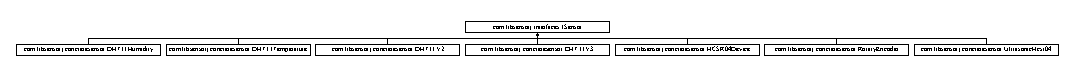
\includegraphics[height=1.216069cm]{interfacecom_1_1libsensorj_1_1interfaces_1_1ISensor}
\end{center}
\end{figure}
\subsection*{Public Member Functions}
\begin{DoxyCompactItemize}
\item 
void \hyperlink{interfacecom_1_1libsensorj_1_1interfaces_1_1ISensor_a3c3db93a33adecde81a528651790f75e}{get\+Instance} ()
\end{DoxyCompactItemize}


\subsection{Member Function Documentation}
\hypertarget{interfacecom_1_1libsensorj_1_1interfaces_1_1ISensor_a3c3db93a33adecde81a528651790f75e}{}\index{com\+::libsensorj\+::interfaces\+::\+I\+Sensor@{com\+::libsensorj\+::interfaces\+::\+I\+Sensor}!get\+Instance@{get\+Instance}}
\index{get\+Instance@{get\+Instance}!com\+::libsensorj\+::interfaces\+::\+I\+Sensor@{com\+::libsensorj\+::interfaces\+::\+I\+Sensor}}
\subsubsection[{get\+Instance}]{\setlength{\rightskip}{0pt plus 5cm}void com.\+libsensorj.\+interfaces.\+I\+Sensor.\+get\+Instance (
\begin{DoxyParamCaption}
{}
\end{DoxyParamCaption}
)}\label{interfacecom_1_1libsensorj_1_1interfaces_1_1ISensor_a3c3db93a33adecde81a528651790f75e}


Implemented in \hyperlink{classcom_1_1libsensorj_1_1concretesensor_1_1DHT11Temperature_a599358623598fb0076dc0a2e07978f0b}{com.\+libsensorj.\+concretesensor.\+D\+H\+T11\+Temperature}, \hyperlink{classcom_1_1libsensorj_1_1concretesensor_1_1UltrasonicHcsr04_a170167614b330d79518647a9a9722b62}{com.\+libsensorj.\+concretesensor.\+Ultrasonic\+Hcsr04}, and \hyperlink{classcom_1_1libsensorj_1_1concretesensor_1_1DHT11Humidity_a2355dc003abad8d519440e9f6871c422}{com.\+libsensorj.\+concretesensor.\+D\+H\+T11\+Humidity}.



The documentation for this interface was generated from the following file\+:\begin{DoxyCompactItemize}
\item 
main/java/com/libsensorj/interfaces/\hyperlink{ISensor_8java}{I\+Sensor.\+java}\end{DoxyCompactItemize}

\hypertarget{interfacecom_1_1libsensorj_1_1interfaces_1_1ISensorFactory}{}\section{com.\+libsensorj.\+interfaces.\+I\+Sensor\+Factory Interface Reference}
\label{interfacecom_1_1libsensorj_1_1interfaces_1_1ISensorFactory}\index{com.\+libsensorj.\+interfaces.\+I\+Sensor\+Factory@{com.\+libsensorj.\+interfaces.\+I\+Sensor\+Factory}}
Inheritance diagram for com.\+libsensorj.\+interfaces.\+I\+Sensor\+Factory\+:\begin{figure}[H]
\begin{center}
\leavevmode
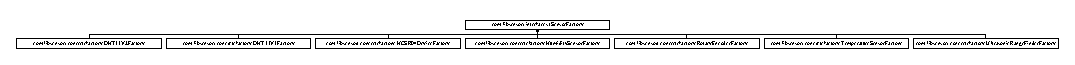
\includegraphics[height=0.430108cm]{interfacecom_1_1libsensorj_1_1interfaces_1_1ISensorFactory}
\end{center}
\end{figure}
\subsection*{Public Member Functions}
\begin{DoxyCompactItemize}
\item 
\hyperlink{interfacecom_1_1libsensorj_1_1interfaces_1_1ISensor}{I\+Sensor} \hyperlink{interfacecom_1_1libsensorj_1_1interfaces_1_1ISensorFactory_ac14c6d566c37c6a79c6db1e85634f25d}{create\+Sensor} ()
\item 
\hyperlink{classcom_1_1libsensorj_1_1interfaces_1_1IEvent}{I\+Event} \hyperlink{interfacecom_1_1libsensorj_1_1interfaces_1_1ISensorFactory_a2b074d01287a4e64677097255ba9e768}{create\+Event} ()
\end{DoxyCompactItemize}


\subsection{Detailed Description}
A factory for creating \hyperlink{interfacecom_1_1libsensorj_1_1interfaces_1_1ISensor}{I\+Sensor} objects. 

\subsection{Member Function Documentation}
\hypertarget{interfacecom_1_1libsensorj_1_1interfaces_1_1ISensorFactory_a2b074d01287a4e64677097255ba9e768}{}\index{com\+::libsensorj\+::interfaces\+::\+I\+Sensor\+Factory@{com\+::libsensorj\+::interfaces\+::\+I\+Sensor\+Factory}!create\+Event@{create\+Event}}
\index{create\+Event@{create\+Event}!com\+::libsensorj\+::interfaces\+::\+I\+Sensor\+Factory@{com\+::libsensorj\+::interfaces\+::\+I\+Sensor\+Factory}}
\subsubsection[{create\+Event}]{\setlength{\rightskip}{0pt plus 5cm}{\bf I\+Event} com.\+libsensorj.\+interfaces.\+I\+Sensor\+Factory.\+create\+Event (
\begin{DoxyParamCaption}
{}
\end{DoxyParamCaption}
)}\label{interfacecom_1_1libsensorj_1_1interfaces_1_1ISensorFactory_a2b074d01287a4e64677097255ba9e768}
Creates a new \hyperlink{classcom_1_1libsensorj_1_1interfaces_1_1IEvent}{I\+Event} object.

\begin{DoxyReturn}{Returns}
the \hyperlink{classcom_1_1libsensorj_1_1interfaces_1_1IEvent}{I\+Event} 
\end{DoxyReturn}


Implemented in \hyperlink{classcom_1_1libsensorj_1_1concretefactory_1_1DHT11V2Factory_a0eb0b480f4133c3eeb2728bd0fa45c58}{com.\+libsensorj.\+concretefactory.\+D\+H\+T11\+V2\+Factory}, \hyperlink{classcom_1_1libsensorj_1_1concretefactory_1_1TemperatureSensorFactory_adb3d5716b5e55f4fc037c0a95ec99688}{com.\+libsensorj.\+concretefactory.\+Temperature\+Sensor\+Factory}, \hyperlink{classcom_1_1libsensorj_1_1concretefactory_1_1HumiditySensorFactory_a43835bfa4c60faf39dfe64f67322b9e4}{com.\+libsensorj.\+concretefactory.\+Humidity\+Sensor\+Factory}, \hyperlink{classcom_1_1libsensorj_1_1concretefactory_1_1DHT11V3Factory_a7621f6dc5c877e6dfb160f68e50fd319}{com.\+libsensorj.\+concretefactory.\+D\+H\+T11\+V3\+Factory}, \hyperlink{classcom_1_1libsensorj_1_1concretefactory_1_1HCSR04DeviceFactory_aea88b0202d3021c4e55bd9cbf64da906}{com.\+libsensorj.\+concretefactory.\+H\+C\+S\+R04\+Device\+Factory}, \hyperlink{classcom_1_1libsensorj_1_1concretefactory_1_1UltrasonicRangeFinderFactory_a8a7d0c55346f1ab5630a878f6a3175fd}{com.\+libsensorj.\+concretefactory.\+Ultrasonic\+Range\+Finder\+Factory}, and \hyperlink{classcom_1_1libsensorj_1_1concretefactory_1_1RotaryEncoderFactory_a8f36c2cbdddcd1c71d438efafc73ffc2}{com.\+libsensorj.\+concretefactory.\+Rotary\+Encoder\+Factory}.

\hypertarget{interfacecom_1_1libsensorj_1_1interfaces_1_1ISensorFactory_ac14c6d566c37c6a79c6db1e85634f25d}{}\index{com\+::libsensorj\+::interfaces\+::\+I\+Sensor\+Factory@{com\+::libsensorj\+::interfaces\+::\+I\+Sensor\+Factory}!create\+Sensor@{create\+Sensor}}
\index{create\+Sensor@{create\+Sensor}!com\+::libsensorj\+::interfaces\+::\+I\+Sensor\+Factory@{com\+::libsensorj\+::interfaces\+::\+I\+Sensor\+Factory}}
\subsubsection[{create\+Sensor}]{\setlength{\rightskip}{0pt plus 5cm}{\bf I\+Sensor} com.\+libsensorj.\+interfaces.\+I\+Sensor\+Factory.\+create\+Sensor (
\begin{DoxyParamCaption}
{}
\end{DoxyParamCaption}
)}\label{interfacecom_1_1libsensorj_1_1interfaces_1_1ISensorFactory_ac14c6d566c37c6a79c6db1e85634f25d}
Creates a new \hyperlink{interfacecom_1_1libsensorj_1_1interfaces_1_1ISensor}{I\+Sensor} object.

\begin{DoxyReturn}{Returns}
the \hyperlink{interfacecom_1_1libsensorj_1_1interfaces_1_1ISensor}{I\+Sensor} 
\end{DoxyReturn}


Implemented in \hyperlink{classcom_1_1libsensorj_1_1concretefactory_1_1DHT11V2Factory_ac04eaebc748d420eb035439dfc1d2202}{com.\+libsensorj.\+concretefactory.\+D\+H\+T11\+V2\+Factory}, \hyperlink{classcom_1_1libsensorj_1_1concretefactory_1_1DHT11V3Factory_ad89c967025d654490729d2f69438805e}{com.\+libsensorj.\+concretefactory.\+D\+H\+T11\+V3\+Factory}, \hyperlink{classcom_1_1libsensorj_1_1concretefactory_1_1HCSR04DeviceFactory_a3d5c07b9ce458a3f56cfe5e7470b51df}{com.\+libsensorj.\+concretefactory.\+H\+C\+S\+R04\+Device\+Factory}, \hyperlink{classcom_1_1libsensorj_1_1concretefactory_1_1HumiditySensorFactory_aec6f80bd08e69d69ea6187067d11d28c}{com.\+libsensorj.\+concretefactory.\+Humidity\+Sensor\+Factory}, \hyperlink{classcom_1_1libsensorj_1_1concretefactory_1_1TemperatureSensorFactory_aeba8598ebe5c182154f63e0c94abdd70}{com.\+libsensorj.\+concretefactory.\+Temperature\+Sensor\+Factory}, \hyperlink{classcom_1_1libsensorj_1_1concretefactory_1_1UltrasonicRangeFinderFactory_a3aa6e46ef47bf97355df4d5cfb1b1e01}{com.\+libsensorj.\+concretefactory.\+Ultrasonic\+Range\+Finder\+Factory}, and \hyperlink{classcom_1_1libsensorj_1_1concretefactory_1_1RotaryEncoderFactory_a5f9c404d9b61d8aaf63cad82b87becd7}{com.\+libsensorj.\+concretefactory.\+Rotary\+Encoder\+Factory}.



The documentation for this interface was generated from the following file\+:\begin{DoxyCompactItemize}
\item 
main/java/com/libsensorj/interfaces/\hyperlink{ISensorFactory_8java}{I\+Sensor\+Factory.\+java}\end{DoxyCompactItemize}

\hypertarget{classcom_1_1pi4j_1_1examples_1_1LcdExample}{}\section{com.\+pi4j.\+examples.\+Lcd\+Example Class Reference}
\label{classcom_1_1pi4j_1_1examples_1_1LcdExample}\index{com.\+pi4j.\+examples.\+Lcd\+Example@{com.\+pi4j.\+examples.\+Lcd\+Example}}
\subsection*{Static Public Member Functions}
\begin{DoxyCompactItemize}
\item 
static void \hyperlink{classcom_1_1pi4j_1_1examples_1_1LcdExample_a09001ffe6860f9ff7d1b9b195eecf3a6}{main} (String\mbox{[}$\,$\mbox{]} args)  throws Interrupted\+Exception 
\end{DoxyCompactItemize}
\subsection*{Static Public Attributes}
\begin{DoxyCompactItemize}
\item 
static final int \hyperlink{classcom_1_1pi4j_1_1examples_1_1LcdExample_aa5552e877b90e91658ff69c91110f97a}{L\+C\+D\+\_\+\+R\+O\+W\+S} = 2
\item 
static final int \hyperlink{classcom_1_1pi4j_1_1examples_1_1LcdExample_a2a8ff60a46f85aba5aa1e31b179825f2}{L\+C\+D\+\_\+\+R\+O\+W\+\_\+1} = 0
\item 
static final int \hyperlink{classcom_1_1pi4j_1_1examples_1_1LcdExample_a05c3899e43e7d71d9effb85603abb271}{L\+C\+D\+\_\+\+R\+O\+W\+\_\+2} = 1
\item 
static final int \hyperlink{classcom_1_1pi4j_1_1examples_1_1LcdExample_a222b7e1bbc25b9da748fcd91edf8da1c}{L\+C\+D\+\_\+\+C\+O\+L\+U\+M\+N\+S} = 16
\item 
static final int \hyperlink{classcom_1_1pi4j_1_1examples_1_1LcdExample_ad2cf111a06d28ba735a13b43347b50b8}{L\+C\+D\+\_\+\+B\+I\+T\+S} = 4
\end{DoxyCompactItemize}
\subsection*{Static Private Attributes}
\begin{DoxyCompactItemize}
\item 
static final String \hyperlink{classcom_1_1pi4j_1_1examples_1_1LcdExample_a1a5efab5ce2806cbf7b512a6c76656c2}{T\+R\+A\+C\+E\+D\+\_\+\+L\+I\+N\+E} = \char`\"{}-\/-\/-\/-\/-\/-\/-\/-\/-\/-\/-\/-\/-\/-\/-\/-\/\char`\"{}
\item 
static final Logger \hyperlink{classcom_1_1pi4j_1_1examples_1_1LcdExample_ac6f94512f51589d4a4e26b46c7688ae1}{L\+O\+G\+G\+E\+R}
\end{DoxyCompactItemize}


\subsection{Member Function Documentation}
\hypertarget{classcom_1_1pi4j_1_1examples_1_1LcdExample_a09001ffe6860f9ff7d1b9b195eecf3a6}{}\index{com\+::pi4j\+::examples\+::\+Lcd\+Example@{com\+::pi4j\+::examples\+::\+Lcd\+Example}!main@{main}}
\index{main@{main}!com\+::pi4j\+::examples\+::\+Lcd\+Example@{com\+::pi4j\+::examples\+::\+Lcd\+Example}}
\subsubsection[{main}]{\setlength{\rightskip}{0pt plus 5cm}static void com.\+pi4j.\+examples.\+Lcd\+Example.\+main (
\begin{DoxyParamCaption}
\item[{String\mbox{[}$\,$\mbox{]}}]{args}
\end{DoxyParamCaption}
) throws Interrupted\+Exception\hspace{0.3cm}{\ttfamily [static]}}\label{classcom_1_1pi4j_1_1examples_1_1LcdExample_a09001ffe6860f9ff7d1b9b195eecf3a6}


\subsection{Member Data Documentation}
\hypertarget{classcom_1_1pi4j_1_1examples_1_1LcdExample_ad2cf111a06d28ba735a13b43347b50b8}{}\index{com\+::pi4j\+::examples\+::\+Lcd\+Example@{com\+::pi4j\+::examples\+::\+Lcd\+Example}!L\+C\+D\+\_\+\+B\+I\+T\+S@{L\+C\+D\+\_\+\+B\+I\+T\+S}}
\index{L\+C\+D\+\_\+\+B\+I\+T\+S@{L\+C\+D\+\_\+\+B\+I\+T\+S}!com\+::pi4j\+::examples\+::\+Lcd\+Example@{com\+::pi4j\+::examples\+::\+Lcd\+Example}}
\subsubsection[{L\+C\+D\+\_\+\+B\+I\+T\+S}]{\setlength{\rightskip}{0pt plus 5cm}final int com.\+pi4j.\+examples.\+Lcd\+Example.\+L\+C\+D\+\_\+\+B\+I\+T\+S = 4\hspace{0.3cm}{\ttfamily [static]}}\label{classcom_1_1pi4j_1_1examples_1_1LcdExample_ad2cf111a06d28ba735a13b43347b50b8}
\hypertarget{classcom_1_1pi4j_1_1examples_1_1LcdExample_a222b7e1bbc25b9da748fcd91edf8da1c}{}\index{com\+::pi4j\+::examples\+::\+Lcd\+Example@{com\+::pi4j\+::examples\+::\+Lcd\+Example}!L\+C\+D\+\_\+\+C\+O\+L\+U\+M\+N\+S@{L\+C\+D\+\_\+\+C\+O\+L\+U\+M\+N\+S}}
\index{L\+C\+D\+\_\+\+C\+O\+L\+U\+M\+N\+S@{L\+C\+D\+\_\+\+C\+O\+L\+U\+M\+N\+S}!com\+::pi4j\+::examples\+::\+Lcd\+Example@{com\+::pi4j\+::examples\+::\+Lcd\+Example}}
\subsubsection[{L\+C\+D\+\_\+\+C\+O\+L\+U\+M\+N\+S}]{\setlength{\rightskip}{0pt plus 5cm}final int com.\+pi4j.\+examples.\+Lcd\+Example.\+L\+C\+D\+\_\+\+C\+O\+L\+U\+M\+N\+S = 16\hspace{0.3cm}{\ttfamily [static]}}\label{classcom_1_1pi4j_1_1examples_1_1LcdExample_a222b7e1bbc25b9da748fcd91edf8da1c}
\hypertarget{classcom_1_1pi4j_1_1examples_1_1LcdExample_a2a8ff60a46f85aba5aa1e31b179825f2}{}\index{com\+::pi4j\+::examples\+::\+Lcd\+Example@{com\+::pi4j\+::examples\+::\+Lcd\+Example}!L\+C\+D\+\_\+\+R\+O\+W\+\_\+1@{L\+C\+D\+\_\+\+R\+O\+W\+\_\+1}}
\index{L\+C\+D\+\_\+\+R\+O\+W\+\_\+1@{L\+C\+D\+\_\+\+R\+O\+W\+\_\+1}!com\+::pi4j\+::examples\+::\+Lcd\+Example@{com\+::pi4j\+::examples\+::\+Lcd\+Example}}
\subsubsection[{L\+C\+D\+\_\+\+R\+O\+W\+\_\+1}]{\setlength{\rightskip}{0pt plus 5cm}final int com.\+pi4j.\+examples.\+Lcd\+Example.\+L\+C\+D\+\_\+\+R\+O\+W\+\_\+1 = 0\hspace{0.3cm}{\ttfamily [static]}}\label{classcom_1_1pi4j_1_1examples_1_1LcdExample_a2a8ff60a46f85aba5aa1e31b179825f2}
\hypertarget{classcom_1_1pi4j_1_1examples_1_1LcdExample_a05c3899e43e7d71d9effb85603abb271}{}\index{com\+::pi4j\+::examples\+::\+Lcd\+Example@{com\+::pi4j\+::examples\+::\+Lcd\+Example}!L\+C\+D\+\_\+\+R\+O\+W\+\_\+2@{L\+C\+D\+\_\+\+R\+O\+W\+\_\+2}}
\index{L\+C\+D\+\_\+\+R\+O\+W\+\_\+2@{L\+C\+D\+\_\+\+R\+O\+W\+\_\+2}!com\+::pi4j\+::examples\+::\+Lcd\+Example@{com\+::pi4j\+::examples\+::\+Lcd\+Example}}
\subsubsection[{L\+C\+D\+\_\+\+R\+O\+W\+\_\+2}]{\setlength{\rightskip}{0pt plus 5cm}final int com.\+pi4j.\+examples.\+Lcd\+Example.\+L\+C\+D\+\_\+\+R\+O\+W\+\_\+2 = 1\hspace{0.3cm}{\ttfamily [static]}}\label{classcom_1_1pi4j_1_1examples_1_1LcdExample_a05c3899e43e7d71d9effb85603abb271}
\hypertarget{classcom_1_1pi4j_1_1examples_1_1LcdExample_aa5552e877b90e91658ff69c91110f97a}{}\index{com\+::pi4j\+::examples\+::\+Lcd\+Example@{com\+::pi4j\+::examples\+::\+Lcd\+Example}!L\+C\+D\+\_\+\+R\+O\+W\+S@{L\+C\+D\+\_\+\+R\+O\+W\+S}}
\index{L\+C\+D\+\_\+\+R\+O\+W\+S@{L\+C\+D\+\_\+\+R\+O\+W\+S}!com\+::pi4j\+::examples\+::\+Lcd\+Example@{com\+::pi4j\+::examples\+::\+Lcd\+Example}}
\subsubsection[{L\+C\+D\+\_\+\+R\+O\+W\+S}]{\setlength{\rightskip}{0pt plus 5cm}final int com.\+pi4j.\+examples.\+Lcd\+Example.\+L\+C\+D\+\_\+\+R\+O\+W\+S = 2\hspace{0.3cm}{\ttfamily [static]}}\label{classcom_1_1pi4j_1_1examples_1_1LcdExample_aa5552e877b90e91658ff69c91110f97a}
\hypertarget{classcom_1_1pi4j_1_1examples_1_1LcdExample_ac6f94512f51589d4a4e26b46c7688ae1}{}\index{com\+::pi4j\+::examples\+::\+Lcd\+Example@{com\+::pi4j\+::examples\+::\+Lcd\+Example}!L\+O\+G\+G\+E\+R@{L\+O\+G\+G\+E\+R}}
\index{L\+O\+G\+G\+E\+R@{L\+O\+G\+G\+E\+R}!com\+::pi4j\+::examples\+::\+Lcd\+Example@{com\+::pi4j\+::examples\+::\+Lcd\+Example}}
\subsubsection[{L\+O\+G\+G\+E\+R}]{\setlength{\rightskip}{0pt plus 5cm}final Logger com.\+pi4j.\+examples.\+Lcd\+Example.\+L\+O\+G\+G\+E\+R\hspace{0.3cm}{\ttfamily [static]}, {\ttfamily [private]}}\label{classcom_1_1pi4j_1_1examples_1_1LcdExample_ac6f94512f51589d4a4e26b46c7688ae1}
{\bfseries Initial value\+:}
\begin{DoxyCode}
= LogManager.getLogger(LcdExample.class
            .getName())
\end{DoxyCode}
\hypertarget{classcom_1_1pi4j_1_1examples_1_1LcdExample_a1a5efab5ce2806cbf7b512a6c76656c2}{}\index{com\+::pi4j\+::examples\+::\+Lcd\+Example@{com\+::pi4j\+::examples\+::\+Lcd\+Example}!T\+R\+A\+C\+E\+D\+\_\+\+L\+I\+N\+E@{T\+R\+A\+C\+E\+D\+\_\+\+L\+I\+N\+E}}
\index{T\+R\+A\+C\+E\+D\+\_\+\+L\+I\+N\+E@{T\+R\+A\+C\+E\+D\+\_\+\+L\+I\+N\+E}!com\+::pi4j\+::examples\+::\+Lcd\+Example@{com\+::pi4j\+::examples\+::\+Lcd\+Example}}
\subsubsection[{T\+R\+A\+C\+E\+D\+\_\+\+L\+I\+N\+E}]{\setlength{\rightskip}{0pt plus 5cm}final String com.\+pi4j.\+examples.\+Lcd\+Example.\+T\+R\+A\+C\+E\+D\+\_\+\+L\+I\+N\+E = \char`\"{}-\/-\/-\/-\/-\/-\/-\/-\/-\/-\/-\/-\/-\/-\/-\/-\/\char`\"{}\hspace{0.3cm}{\ttfamily [static]}, {\ttfamily [private]}}\label{classcom_1_1pi4j_1_1examples_1_1LcdExample_a1a5efab5ce2806cbf7b512a6c76656c2}


The documentation for this class was generated from the following file\+:\begin{DoxyCompactItemize}
\item 
main/java/com/pi4j/examples/\hyperlink{LcdExample_8java}{Lcd\+Example.\+java}\end{DoxyCompactItemize}

\hypertarget{classcom_1_1pi4j_1_1examples_1_1ListenGpioExample}{}\section{com.\+pi4j.\+examples.\+Listen\+Gpio\+Example Class Reference}
\label{classcom_1_1pi4j_1_1examples_1_1ListenGpioExample}\index{com.\+pi4j.\+examples.\+Listen\+Gpio\+Example@{com.\+pi4j.\+examples.\+Listen\+Gpio\+Example}}
\subsection*{Static Public Member Functions}
\begin{DoxyCompactItemize}
\item 
static void \hyperlink{classcom_1_1pi4j_1_1examples_1_1ListenGpioExample_af151921c77a802d79eaeb99dca17f99a}{main} (String\mbox{[}$\,$\mbox{]} args)  throws Interrupted\+Exception 
\end{DoxyCompactItemize}
\subsection*{Static Private Attributes}
\begin{DoxyCompactItemize}
\item 
static final Logger \hyperlink{classcom_1_1pi4j_1_1examples_1_1ListenGpioExample_aff41cf086d718e409d352e9e88ba4523}{L\+O\+G\+G\+E\+R}
\end{DoxyCompactItemize}


\subsection{Detailed Description}
This example code demonstrates how to setup a listener for G\+P\+I\+O pin state changes on the Raspberry Pi.

\begin{DoxyAuthor}{Author}
Robert Savage 
\end{DoxyAuthor}


\subsection{Member Function Documentation}
\hypertarget{classcom_1_1pi4j_1_1examples_1_1ListenGpioExample_af151921c77a802d79eaeb99dca17f99a}{}\index{com\+::pi4j\+::examples\+::\+Listen\+Gpio\+Example@{com\+::pi4j\+::examples\+::\+Listen\+Gpio\+Example}!main@{main}}
\index{main@{main}!com\+::pi4j\+::examples\+::\+Listen\+Gpio\+Example@{com\+::pi4j\+::examples\+::\+Listen\+Gpio\+Example}}
\subsubsection[{main}]{\setlength{\rightskip}{0pt plus 5cm}static void com.\+pi4j.\+examples.\+Listen\+Gpio\+Example.\+main (
\begin{DoxyParamCaption}
\item[{String\mbox{[}$\,$\mbox{]}}]{args}
\end{DoxyParamCaption}
) throws Interrupted\+Exception\hspace{0.3cm}{\ttfamily [static]}}\label{classcom_1_1pi4j_1_1examples_1_1ListenGpioExample_af151921c77a802d79eaeb99dca17f99a}


\subsection{Member Data Documentation}
\hypertarget{classcom_1_1pi4j_1_1examples_1_1ListenGpioExample_aff41cf086d718e409d352e9e88ba4523}{}\index{com\+::pi4j\+::examples\+::\+Listen\+Gpio\+Example@{com\+::pi4j\+::examples\+::\+Listen\+Gpio\+Example}!L\+O\+G\+G\+E\+R@{L\+O\+G\+G\+E\+R}}
\index{L\+O\+G\+G\+E\+R@{L\+O\+G\+G\+E\+R}!com\+::pi4j\+::examples\+::\+Listen\+Gpio\+Example@{com\+::pi4j\+::examples\+::\+Listen\+Gpio\+Example}}
\subsubsection[{L\+O\+G\+G\+E\+R}]{\setlength{\rightskip}{0pt plus 5cm}final Logger com.\+pi4j.\+examples.\+Listen\+Gpio\+Example.\+L\+O\+G\+G\+E\+R\hspace{0.3cm}{\ttfamily [static]}, {\ttfamily [private]}}\label{classcom_1_1pi4j_1_1examples_1_1ListenGpioExample_aff41cf086d718e409d352e9e88ba4523}
{\bfseries Initial value\+:}
\begin{DoxyCode}
= LogManager
            .getLogger(ListenGpioExample.class.getName())
\end{DoxyCode}


The documentation for this class was generated from the following file\+:\begin{DoxyCompactItemize}
\item 
main/java/com/pi4j/examples/\hyperlink{ListenGpioExample_8java}{Listen\+Gpio\+Example.\+java}\end{DoxyCompactItemize}

\hypertarget{classcom_1_1pi4j_1_1examples_1_1ListenMultipleGpioExample}{}\section{com.\+pi4j.\+examples.\+Listen\+Multiple\+Gpio\+Example Class Reference}
\label{classcom_1_1pi4j_1_1examples_1_1ListenMultipleGpioExample}\index{com.\+pi4j.\+examples.\+Listen\+Multiple\+Gpio\+Example@{com.\+pi4j.\+examples.\+Listen\+Multiple\+Gpio\+Example}}
\subsection*{Static Public Member Functions}
\begin{DoxyCompactItemize}
\item 
static void \hyperlink{classcom_1_1pi4j_1_1examples_1_1ListenMultipleGpioExample_a3d6b2b26105dee97222637a46edfb137}{main} (String\mbox{[}$\,$\mbox{]} args)  throws Interrupted\+Exception 
\end{DoxyCompactItemize}
\subsection*{Static Private Attributes}
\begin{DoxyCompactItemize}
\item 
static final Logger \hyperlink{classcom_1_1pi4j_1_1examples_1_1ListenMultipleGpioExample_a2ed4104703cde24426579ecec39f2a33}{L\+O\+G\+G\+E\+R}
\end{DoxyCompactItemize}


\subsection{Detailed Description}
This example code demonstrates how to setup a listener for G\+P\+I\+O pin state changes on the Raspberry Pi.

\begin{DoxyAuthor}{Author}
Robert Savage 
\end{DoxyAuthor}


\subsection{Member Function Documentation}
\hypertarget{classcom_1_1pi4j_1_1examples_1_1ListenMultipleGpioExample_a3d6b2b26105dee97222637a46edfb137}{}\index{com\+::pi4j\+::examples\+::\+Listen\+Multiple\+Gpio\+Example@{com\+::pi4j\+::examples\+::\+Listen\+Multiple\+Gpio\+Example}!main@{main}}
\index{main@{main}!com\+::pi4j\+::examples\+::\+Listen\+Multiple\+Gpio\+Example@{com\+::pi4j\+::examples\+::\+Listen\+Multiple\+Gpio\+Example}}
\subsubsection[{main}]{\setlength{\rightskip}{0pt plus 5cm}static void com.\+pi4j.\+examples.\+Listen\+Multiple\+Gpio\+Example.\+main (
\begin{DoxyParamCaption}
\item[{String\mbox{[}$\,$\mbox{]}}]{args}
\end{DoxyParamCaption}
) throws Interrupted\+Exception\hspace{0.3cm}{\ttfamily [static]}}\label{classcom_1_1pi4j_1_1examples_1_1ListenMultipleGpioExample_a3d6b2b26105dee97222637a46edfb137}


\subsection{Member Data Documentation}
\hypertarget{classcom_1_1pi4j_1_1examples_1_1ListenMultipleGpioExample_a2ed4104703cde24426579ecec39f2a33}{}\index{com\+::pi4j\+::examples\+::\+Listen\+Multiple\+Gpio\+Example@{com\+::pi4j\+::examples\+::\+Listen\+Multiple\+Gpio\+Example}!L\+O\+G\+G\+E\+R@{L\+O\+G\+G\+E\+R}}
\index{L\+O\+G\+G\+E\+R@{L\+O\+G\+G\+E\+R}!com\+::pi4j\+::examples\+::\+Listen\+Multiple\+Gpio\+Example@{com\+::pi4j\+::examples\+::\+Listen\+Multiple\+Gpio\+Example}}
\subsubsection[{L\+O\+G\+G\+E\+R}]{\setlength{\rightskip}{0pt plus 5cm}final Logger com.\+pi4j.\+examples.\+Listen\+Multiple\+Gpio\+Example.\+L\+O\+G\+G\+E\+R\hspace{0.3cm}{\ttfamily [static]}, {\ttfamily [private]}}\label{classcom_1_1pi4j_1_1examples_1_1ListenMultipleGpioExample_a2ed4104703cde24426579ecec39f2a33}
{\bfseries Initial value\+:}
\begin{DoxyCode}
= LogManager
            .getLogger(ListenMultipleGpioExample.class.getName())
\end{DoxyCode}


The documentation for this class was generated from the following file\+:\begin{DoxyCompactItemize}
\item 
main/java/com/pi4j/examples/\hyperlink{ListenMultipleGpioExample_8java}{Listen\+Multiple\+Gpio\+Example.\+java}\end{DoxyCompactItemize}

\hypertarget{classcom_1_1pi4j_1_1examples_1_1MCP23017GpioExample}{}\section{com.\+pi4j.\+examples.\+M\+C\+P23017\+Gpio\+Example Class Reference}
\label{classcom_1_1pi4j_1_1examples_1_1MCP23017GpioExample}\index{com.\+pi4j.\+examples.\+M\+C\+P23017\+Gpio\+Example@{com.\+pi4j.\+examples.\+M\+C\+P23017\+Gpio\+Example}}
\subsection*{Static Public Member Functions}
\begin{DoxyCompactItemize}
\item 
static void \hyperlink{classcom_1_1pi4j_1_1examples_1_1MCP23017GpioExample_adde74bf11cb8efcef4c15ed3a9a546b2}{main} (String\mbox{[}$\,$\mbox{]} args)  throws Interrupted\+Exception,             I\+O\+Exception 
\end{DoxyCompactItemize}
\subsection*{Static Private Attributes}
\begin{DoxyCompactItemize}
\item 
static final Logger \hyperlink{classcom_1_1pi4j_1_1examples_1_1MCP23017GpioExample_a4d89402b7b53544ff7c38be922407217}{L\+O\+G\+G\+E\+R}
\end{DoxyCompactItemize}


\subsection{Detailed Description}
This example code demonstrates how to setup a custom Gpio\+Provider for G\+P\+I\+O pin state control and monitoring. 

This example implements the M\+C\+P23017 G\+P\+I\+O expansion board. More information about the board can be found here\+: $\ast$ \href{http://ww1.microchip.com/downloads/en/DeviceDoc/21952b.pdf}{\tt http\+://ww1.\+microchip.\+com/downloads/en/\+Device\+Doc/21952b.\+pdf} 

The M\+C\+P23017 is connected via I2\+C connection to the Raspberry Pi and provides 16 G\+P\+I\+O pins that can be used for either digital input or digital output pins. 

\begin{DoxyAuthor}{Author}
Robert Savage 
\end{DoxyAuthor}


\subsection{Member Function Documentation}
\hypertarget{classcom_1_1pi4j_1_1examples_1_1MCP23017GpioExample_adde74bf11cb8efcef4c15ed3a9a546b2}{}\index{com\+::pi4j\+::examples\+::\+M\+C\+P23017\+Gpio\+Example@{com\+::pi4j\+::examples\+::\+M\+C\+P23017\+Gpio\+Example}!main@{main}}
\index{main@{main}!com\+::pi4j\+::examples\+::\+M\+C\+P23017\+Gpio\+Example@{com\+::pi4j\+::examples\+::\+M\+C\+P23017\+Gpio\+Example}}
\subsubsection[{main}]{\setlength{\rightskip}{0pt plus 5cm}static void com.\+pi4j.\+examples.\+M\+C\+P23017\+Gpio\+Example.\+main (
\begin{DoxyParamCaption}
\item[{String\mbox{[}$\,$\mbox{]}}]{args}
\end{DoxyParamCaption}
) throws Interrupted\+Exception,             I\+O\+Exception\hspace{0.3cm}{\ttfamily [static]}}\label{classcom_1_1pi4j_1_1examples_1_1MCP23017GpioExample_adde74bf11cb8efcef4c15ed3a9a546b2}


\subsection{Member Data Documentation}
\hypertarget{classcom_1_1pi4j_1_1examples_1_1MCP23017GpioExample_a4d89402b7b53544ff7c38be922407217}{}\index{com\+::pi4j\+::examples\+::\+M\+C\+P23017\+Gpio\+Example@{com\+::pi4j\+::examples\+::\+M\+C\+P23017\+Gpio\+Example}!L\+O\+G\+G\+E\+R@{L\+O\+G\+G\+E\+R}}
\index{L\+O\+G\+G\+E\+R@{L\+O\+G\+G\+E\+R}!com\+::pi4j\+::examples\+::\+M\+C\+P23017\+Gpio\+Example@{com\+::pi4j\+::examples\+::\+M\+C\+P23017\+Gpio\+Example}}
\subsubsection[{L\+O\+G\+G\+E\+R}]{\setlength{\rightskip}{0pt plus 5cm}final Logger com.\+pi4j.\+examples.\+M\+C\+P23017\+Gpio\+Example.\+L\+O\+G\+G\+E\+R\hspace{0.3cm}{\ttfamily [static]}, {\ttfamily [private]}}\label{classcom_1_1pi4j_1_1examples_1_1MCP23017GpioExample_a4d89402b7b53544ff7c38be922407217}
{\bfseries Initial value\+:}
\begin{DoxyCode}
= LogManager
            .getLogger(MCP23017GpioExample.class.getName())
\end{DoxyCode}


The documentation for this class was generated from the following file\+:\begin{DoxyCompactItemize}
\item 
main/java/com/pi4j/examples/\hyperlink{MCP23017GpioExample_8java}{M\+C\+P23017\+Gpio\+Example.\+java}\end{DoxyCompactItemize}

\hypertarget{classcom_1_1pi4j_1_1examples_1_1MCP23S17GpioExample}{}\section{com.\+pi4j.\+examples.\+M\+C\+P23\+S17\+Gpio\+Example Class Reference}
\label{classcom_1_1pi4j_1_1examples_1_1MCP23S17GpioExample}\index{com.\+pi4j.\+examples.\+M\+C\+P23\+S17\+Gpio\+Example@{com.\+pi4j.\+examples.\+M\+C\+P23\+S17\+Gpio\+Example}}
\subsection*{Static Public Member Functions}
\begin{DoxyCompactItemize}
\item 
static void \hyperlink{classcom_1_1pi4j_1_1examples_1_1MCP23S17GpioExample_a3896e28c5614767481cd2ac6534ddb28}{main} (String\mbox{[}$\,$\mbox{]} args)  throws Interrupted\+Exception,             I\+O\+Exception 
\end{DoxyCompactItemize}
\subsection*{Static Private Attributes}
\begin{DoxyCompactItemize}
\item 
static final Logger \hyperlink{classcom_1_1pi4j_1_1examples_1_1MCP23S17GpioExample_a89341794ca51e5d836996686d7629055}{L\+O\+G\+G\+E\+R}
\end{DoxyCompactItemize}


\subsection{Detailed Description}
This example code demonstrates how to setup a custom Gpio\+Provider for G\+P\+I\+O pin state control and monitoring. 

This example implements the M\+C\+P23\+S17 G\+P\+I\+O expansion board. More information about the board can be found here\+: $\ast$ \href{http://ww1.microchip.com/downloads/en/DeviceDoc/21952b.pdf}{\tt http\+://ww1.\+microchip.\+com/downloads/en/\+Device\+Doc/21952b.\+pdf} 

The M\+C\+P23\+S17 is connected via S\+P\+I connection to the Raspberry Pi and provides 16 G\+P\+I\+O pins that can be used for either digital input or digital output pins. 

\begin{DoxyAuthor}{Author}
Robert Savage 
\end{DoxyAuthor}


\subsection{Member Function Documentation}
\hypertarget{classcom_1_1pi4j_1_1examples_1_1MCP23S17GpioExample_a3896e28c5614767481cd2ac6534ddb28}{}\index{com\+::pi4j\+::examples\+::\+M\+C\+P23\+S17\+Gpio\+Example@{com\+::pi4j\+::examples\+::\+M\+C\+P23\+S17\+Gpio\+Example}!main@{main}}
\index{main@{main}!com\+::pi4j\+::examples\+::\+M\+C\+P23\+S17\+Gpio\+Example@{com\+::pi4j\+::examples\+::\+M\+C\+P23\+S17\+Gpio\+Example}}
\subsubsection[{main}]{\setlength{\rightskip}{0pt plus 5cm}static void com.\+pi4j.\+examples.\+M\+C\+P23\+S17\+Gpio\+Example.\+main (
\begin{DoxyParamCaption}
\item[{String\mbox{[}$\,$\mbox{]}}]{args}
\end{DoxyParamCaption}
) throws Interrupted\+Exception,             I\+O\+Exception\hspace{0.3cm}{\ttfamily [static]}}\label{classcom_1_1pi4j_1_1examples_1_1MCP23S17GpioExample_a3896e28c5614767481cd2ac6534ddb28}


\subsection{Member Data Documentation}
\hypertarget{classcom_1_1pi4j_1_1examples_1_1MCP23S17GpioExample_a89341794ca51e5d836996686d7629055}{}\index{com\+::pi4j\+::examples\+::\+M\+C\+P23\+S17\+Gpio\+Example@{com\+::pi4j\+::examples\+::\+M\+C\+P23\+S17\+Gpio\+Example}!L\+O\+G\+G\+E\+R@{L\+O\+G\+G\+E\+R}}
\index{L\+O\+G\+G\+E\+R@{L\+O\+G\+G\+E\+R}!com\+::pi4j\+::examples\+::\+M\+C\+P23\+S17\+Gpio\+Example@{com\+::pi4j\+::examples\+::\+M\+C\+P23\+S17\+Gpio\+Example}}
\subsubsection[{L\+O\+G\+G\+E\+R}]{\setlength{\rightskip}{0pt plus 5cm}final Logger com.\+pi4j.\+examples.\+M\+C\+P23\+S17\+Gpio\+Example.\+L\+O\+G\+G\+E\+R\hspace{0.3cm}{\ttfamily [static]}, {\ttfamily [private]}}\label{classcom_1_1pi4j_1_1examples_1_1MCP23S17GpioExample_a89341794ca51e5d836996686d7629055}
{\bfseries Initial value\+:}
\begin{DoxyCode}
= LogManager
            .getLogger(MCP23S17GpioExample.class.getName())
\end{DoxyCode}


The documentation for this class was generated from the following file\+:\begin{DoxyCompactItemize}
\item 
main/java/com/pi4j/examples/\hyperlink{MCP23S17GpioExample_8java}{M\+C\+P23\+S17\+Gpio\+Example.\+java}\end{DoxyCompactItemize}

\hypertarget{classcom_1_1pi4j_1_1examples_1_1MCP4725GpioExample}{}\section{com.\+pi4j.\+examples.\+M\+C\+P4725\+Gpio\+Example Class Reference}
\label{classcom_1_1pi4j_1_1examples_1_1MCP4725GpioExample}\index{com.\+pi4j.\+examples.\+M\+C\+P4725\+Gpio\+Example@{com.\+pi4j.\+examples.\+M\+C\+P4725\+Gpio\+Example}}
\subsection*{Static Public Member Functions}
\begin{DoxyCompactItemize}
\item 
static void \hyperlink{classcom_1_1pi4j_1_1examples_1_1MCP4725GpioExample_a2160bb6445ca5002a3f70f042817b869}{main} (String\mbox{[}$\,$\mbox{]} args)  throws Exception 
\end{DoxyCompactItemize}
\subsection*{Static Private Attributes}
\begin{DoxyCompactItemize}
\item 
static final Logger \hyperlink{classcom_1_1pi4j_1_1examples_1_1MCP4725GpioExample_a08fe11ede756c66903f659463cab8cbc}{L\+O\+G\+G\+E\+R}
\end{DoxyCompactItemize}


\subsection{Detailed Description}
This example code demonstrates how to setup a custom Gpio\+Provider for analog output pin. 

This G\+P\+I\+O provider implements the M\+C\+P4725 12-\/\+Bit Digital-\/to-\/\+Analog Converter as native Pi4\+J G\+P\+I\+O pins. More information about the board can be found here\+: \href{http://http://www.adafruit.com/product/935}{\tt http\+://http\+://www.\+adafruit.\+com/product/935} 

The M\+C\+P4725 is connected via S\+P\+I connection to the Raspberry Pi and provides 1 G\+P\+I\+O analog output pin. 

\begin{DoxyAuthor}{Author}
Christian Wehrli 
\end{DoxyAuthor}


\subsection{Member Function Documentation}
\hypertarget{classcom_1_1pi4j_1_1examples_1_1MCP4725GpioExample_a2160bb6445ca5002a3f70f042817b869}{}\index{com\+::pi4j\+::examples\+::\+M\+C\+P4725\+Gpio\+Example@{com\+::pi4j\+::examples\+::\+M\+C\+P4725\+Gpio\+Example}!main@{main}}
\index{main@{main}!com\+::pi4j\+::examples\+::\+M\+C\+P4725\+Gpio\+Example@{com\+::pi4j\+::examples\+::\+M\+C\+P4725\+Gpio\+Example}}
\subsubsection[{main}]{\setlength{\rightskip}{0pt plus 5cm}static void com.\+pi4j.\+examples.\+M\+C\+P4725\+Gpio\+Example.\+main (
\begin{DoxyParamCaption}
\item[{String\mbox{[}$\,$\mbox{]}}]{args}
\end{DoxyParamCaption}
) throws Exception\hspace{0.3cm}{\ttfamily [static]}}\label{classcom_1_1pi4j_1_1examples_1_1MCP4725GpioExample_a2160bb6445ca5002a3f70f042817b869}


\subsection{Member Data Documentation}
\hypertarget{classcom_1_1pi4j_1_1examples_1_1MCP4725GpioExample_a08fe11ede756c66903f659463cab8cbc}{}\index{com\+::pi4j\+::examples\+::\+M\+C\+P4725\+Gpio\+Example@{com\+::pi4j\+::examples\+::\+M\+C\+P4725\+Gpio\+Example}!L\+O\+G\+G\+E\+R@{L\+O\+G\+G\+E\+R}}
\index{L\+O\+G\+G\+E\+R@{L\+O\+G\+G\+E\+R}!com\+::pi4j\+::examples\+::\+M\+C\+P4725\+Gpio\+Example@{com\+::pi4j\+::examples\+::\+M\+C\+P4725\+Gpio\+Example}}
\subsubsection[{L\+O\+G\+G\+E\+R}]{\setlength{\rightskip}{0pt plus 5cm}final Logger com.\+pi4j.\+examples.\+M\+C\+P4725\+Gpio\+Example.\+L\+O\+G\+G\+E\+R\hspace{0.3cm}{\ttfamily [static]}, {\ttfamily [private]}}\label{classcom_1_1pi4j_1_1examples_1_1MCP4725GpioExample_a08fe11ede756c66903f659463cab8cbc}
{\bfseries Initial value\+:}
\begin{DoxyCode}
= LogManager
            .getLogger(MCP4725GpioExample.class.getName())
\end{DoxyCode}


The documentation for this class was generated from the following file\+:\begin{DoxyCompactItemize}
\item 
main/java/com/pi4j/examples/\hyperlink{MCP4725GpioExample_8java}{M\+C\+P4725\+Gpio\+Example.\+java}\end{DoxyCompactItemize}

\hypertarget{classcom_1_1pi4j_1_1examples_1_1MultipurposePinGpioExample}{}\section{com.\+pi4j.\+examples.\+Multipurpose\+Pin\+Gpio\+Example Class Reference}
\label{classcom_1_1pi4j_1_1examples_1_1MultipurposePinGpioExample}\index{com.\+pi4j.\+examples.\+Multipurpose\+Pin\+Gpio\+Example@{com.\+pi4j.\+examples.\+Multipurpose\+Pin\+Gpio\+Example}}
\subsection*{Static Public Member Functions}
\begin{DoxyCompactItemize}
\item 
static void \hyperlink{classcom_1_1pi4j_1_1examples_1_1MultipurposePinGpioExample_a7e30237e1014da090db9da21801b2ee9}{main} (String\mbox{[}$\,$\mbox{]} args)  throws Interrupted\+Exception 
\end{DoxyCompactItemize}
\subsection*{Static Private Attributes}
\begin{DoxyCompactItemize}
\item 
static final Logger \hyperlink{classcom_1_1pi4j_1_1examples_1_1MultipurposePinGpioExample_a9a1347f7e0ff65f61938faa256526811}{L\+O\+G\+G\+E\+R}
\end{DoxyCompactItemize}


\subsection{Detailed Description}
This example code demonstrates how to setup a multi-\/purpose digital pin on the Raspberry Pi.

\begin{DoxyAuthor}{Author}
Robert Savage 
\end{DoxyAuthor}


\subsection{Member Function Documentation}
\hypertarget{classcom_1_1pi4j_1_1examples_1_1MultipurposePinGpioExample_a7e30237e1014da090db9da21801b2ee9}{}\index{com\+::pi4j\+::examples\+::\+Multipurpose\+Pin\+Gpio\+Example@{com\+::pi4j\+::examples\+::\+Multipurpose\+Pin\+Gpio\+Example}!main@{main}}
\index{main@{main}!com\+::pi4j\+::examples\+::\+Multipurpose\+Pin\+Gpio\+Example@{com\+::pi4j\+::examples\+::\+Multipurpose\+Pin\+Gpio\+Example}}
\subsubsection[{main}]{\setlength{\rightskip}{0pt plus 5cm}static void com.\+pi4j.\+examples.\+Multipurpose\+Pin\+Gpio\+Example.\+main (
\begin{DoxyParamCaption}
\item[{String\mbox{[}$\,$\mbox{]}}]{args}
\end{DoxyParamCaption}
) throws Interrupted\+Exception\hspace{0.3cm}{\ttfamily [static]}}\label{classcom_1_1pi4j_1_1examples_1_1MultipurposePinGpioExample_a7e30237e1014da090db9da21801b2ee9}


\subsection{Member Data Documentation}
\hypertarget{classcom_1_1pi4j_1_1examples_1_1MultipurposePinGpioExample_a9a1347f7e0ff65f61938faa256526811}{}\index{com\+::pi4j\+::examples\+::\+Multipurpose\+Pin\+Gpio\+Example@{com\+::pi4j\+::examples\+::\+Multipurpose\+Pin\+Gpio\+Example}!L\+O\+G\+G\+E\+R@{L\+O\+G\+G\+E\+R}}
\index{L\+O\+G\+G\+E\+R@{L\+O\+G\+G\+E\+R}!com\+::pi4j\+::examples\+::\+Multipurpose\+Pin\+Gpio\+Example@{com\+::pi4j\+::examples\+::\+Multipurpose\+Pin\+Gpio\+Example}}
\subsubsection[{L\+O\+G\+G\+E\+R}]{\setlength{\rightskip}{0pt plus 5cm}final Logger com.\+pi4j.\+examples.\+Multipurpose\+Pin\+Gpio\+Example.\+L\+O\+G\+G\+E\+R\hspace{0.3cm}{\ttfamily [static]}, {\ttfamily [private]}}\label{classcom_1_1pi4j_1_1examples_1_1MultipurposePinGpioExample_a9a1347f7e0ff65f61938faa256526811}
{\bfseries Initial value\+:}
\begin{DoxyCode}
= LogManager
            .getLogger(MultipurposePinGpioExample.class.getName())
\end{DoxyCode}


The documentation for this class was generated from the following file\+:\begin{DoxyCompactItemize}
\item 
main/java/com/pi4j/examples/\hyperlink{MultipurposePinGpioExample_8java}{Multipurpose\+Pin\+Gpio\+Example.\+java}\end{DoxyCompactItemize}

\hypertarget{classcom_1_1pi4j_1_1examples_1_1MyExample}{}\section{com.\+pi4j.\+examples.\+My\+Example Class Reference}
\label{classcom_1_1pi4j_1_1examples_1_1MyExample}\index{com.\+pi4j.\+examples.\+My\+Example@{com.\+pi4j.\+examples.\+My\+Example}}
\subsection*{Static Public Member Functions}
\begin{DoxyCompactItemize}
\item 
static void \hyperlink{classcom_1_1pi4j_1_1examples_1_1MyExample_a535756901ce4a1b547faf38117a3ec6f}{main} (String\mbox{[}$\,$\mbox{]} args)
\end{DoxyCompactItemize}


\subsection{Detailed Description}
The Class \hyperlink{classcom_1_1pi4j_1_1examples_1_1MyExample}{My\+Example}. 

\subsection{Member Function Documentation}
\hypertarget{classcom_1_1pi4j_1_1examples_1_1MyExample_a535756901ce4a1b547faf38117a3ec6f}{}\index{com\+::pi4j\+::examples\+::\+My\+Example@{com\+::pi4j\+::examples\+::\+My\+Example}!main@{main}}
\index{main@{main}!com\+::pi4j\+::examples\+::\+My\+Example@{com\+::pi4j\+::examples\+::\+My\+Example}}
\subsubsection[{main}]{\setlength{\rightskip}{0pt plus 5cm}static void com.\+pi4j.\+examples.\+My\+Example.\+main (
\begin{DoxyParamCaption}
\item[{String\mbox{[}$\,$\mbox{]}}]{args}
\end{DoxyParamCaption}
)\hspace{0.3cm}{\ttfamily [static]}}\label{classcom_1_1pi4j_1_1examples_1_1MyExample_a535756901ce4a1b547faf38117a3ec6f}
The main method.


\begin{DoxyParams}{Parameters}
{\em args} & the arguments \\
\hline
\end{DoxyParams}


The documentation for this class was generated from the following file\+:\begin{DoxyCompactItemize}
\item 
main/java/com/pi4j/examples/\hyperlink{MyExample_8java}{My\+Example.\+java}\end{DoxyCompactItemize}

\hypertarget{classcom_1_1libsensorj_1_1model_1_1Observer}{}\section{com.\+libsensorj.\+model.\+Observer Class Reference}
\label{classcom_1_1libsensorj_1_1model_1_1Observer}\index{com.\+libsensorj.\+model.\+Observer@{com.\+libsensorj.\+model.\+Observer}}
\subsection*{Public Member Functions}
\begin{DoxyCompactItemize}
\item 
\hyperlink{classcom_1_1libsensorj_1_1model_1_1Observer_a477725e32a58d3a8762d404799ec0161}{Observer} ()
\item 
\hyperlink{classcom_1_1libsensorj_1_1model_1_1Observer_a4933adee4c8da771eaa94415f6f840a7}{Observer} (String \hyperlink{classcom_1_1libsensorj_1_1model_1_1Observer_aa1f9da7634c35f34d5f20d5bc1562428}{observer\+Name})
\item 
String \hyperlink{classcom_1_1libsensorj_1_1model_1_1Observer_a8b873b9c90ad7f1ed055ea6713e0062a}{get\+Observer\+Name} ()
\item 
void \hyperlink{classcom_1_1libsensorj_1_1model_1_1Observer_a42628ca2b4d99e0df9fe1d70fec811b2}{set\+Observer\+Name} (String \hyperlink{classcom_1_1libsensorj_1_1model_1_1Observer_aa1f9da7634c35f34d5f20d5bc1562428}{observer\+Name})
\end{DoxyCompactItemize}
\subsection*{Private Attributes}
\begin{DoxyCompactItemize}
\item 
String \hyperlink{classcom_1_1libsensorj_1_1model_1_1Observer_aa1f9da7634c35f34d5f20d5bc1562428}{observer\+Name}
\end{DoxyCompactItemize}


\subsection{Detailed Description}
The Class \hyperlink{classcom_1_1libsensorj_1_1model_1_1Observer}{Observer}. 

\subsection{Constructor \& Destructor Documentation}
\hypertarget{classcom_1_1libsensorj_1_1model_1_1Observer_a477725e32a58d3a8762d404799ec0161}{}\index{com\+::libsensorj\+::model\+::\+Observer@{com\+::libsensorj\+::model\+::\+Observer}!Observer@{Observer}}
\index{Observer@{Observer}!com\+::libsensorj\+::model\+::\+Observer@{com\+::libsensorj\+::model\+::\+Observer}}
\subsubsection[{Observer}]{\setlength{\rightskip}{0pt plus 5cm}com.\+libsensorj.\+model.\+Observer.\+Observer (
\begin{DoxyParamCaption}
{}
\end{DoxyParamCaption}
)}\label{classcom_1_1libsensorj_1_1model_1_1Observer_a477725e32a58d3a8762d404799ec0161}
Instantiates a new observer. \hypertarget{classcom_1_1libsensorj_1_1model_1_1Observer_a4933adee4c8da771eaa94415f6f840a7}{}\index{com\+::libsensorj\+::model\+::\+Observer@{com\+::libsensorj\+::model\+::\+Observer}!Observer@{Observer}}
\index{Observer@{Observer}!com\+::libsensorj\+::model\+::\+Observer@{com\+::libsensorj\+::model\+::\+Observer}}
\subsubsection[{Observer}]{\setlength{\rightskip}{0pt plus 5cm}com.\+libsensorj.\+model.\+Observer.\+Observer (
\begin{DoxyParamCaption}
\item[{String}]{observer\+Name}
\end{DoxyParamCaption}
)}\label{classcom_1_1libsensorj_1_1model_1_1Observer_a4933adee4c8da771eaa94415f6f840a7}
Instantiates a new observer.


\begin{DoxyParams}{Parameters}
{\em observer\+Name} & the observer name \\
\hline
\end{DoxyParams}


\subsection{Member Function Documentation}
\hypertarget{classcom_1_1libsensorj_1_1model_1_1Observer_a8b873b9c90ad7f1ed055ea6713e0062a}{}\index{com\+::libsensorj\+::model\+::\+Observer@{com\+::libsensorj\+::model\+::\+Observer}!get\+Observer\+Name@{get\+Observer\+Name}}
\index{get\+Observer\+Name@{get\+Observer\+Name}!com\+::libsensorj\+::model\+::\+Observer@{com\+::libsensorj\+::model\+::\+Observer}}
\subsubsection[{get\+Observer\+Name}]{\setlength{\rightskip}{0pt plus 5cm}String com.\+libsensorj.\+model.\+Observer.\+get\+Observer\+Name (
\begin{DoxyParamCaption}
{}
\end{DoxyParamCaption}
)}\label{classcom_1_1libsensorj_1_1model_1_1Observer_a8b873b9c90ad7f1ed055ea6713e0062a}
Gets the observer name.

\begin{DoxyReturn}{Returns}
the observer name 
\end{DoxyReturn}
\hypertarget{classcom_1_1libsensorj_1_1model_1_1Observer_a42628ca2b4d99e0df9fe1d70fec811b2}{}\index{com\+::libsensorj\+::model\+::\+Observer@{com\+::libsensorj\+::model\+::\+Observer}!set\+Observer\+Name@{set\+Observer\+Name}}
\index{set\+Observer\+Name@{set\+Observer\+Name}!com\+::libsensorj\+::model\+::\+Observer@{com\+::libsensorj\+::model\+::\+Observer}}
\subsubsection[{set\+Observer\+Name}]{\setlength{\rightskip}{0pt plus 5cm}void com.\+libsensorj.\+model.\+Observer.\+set\+Observer\+Name (
\begin{DoxyParamCaption}
\item[{String}]{observer\+Name}
\end{DoxyParamCaption}
)}\label{classcom_1_1libsensorj_1_1model_1_1Observer_a42628ca2b4d99e0df9fe1d70fec811b2}
Sets the observer name.


\begin{DoxyParams}{Parameters}
{\em observer\+Name} & the new observer name \\
\hline
\end{DoxyParams}


\subsection{Member Data Documentation}
\hypertarget{classcom_1_1libsensorj_1_1model_1_1Observer_aa1f9da7634c35f34d5f20d5bc1562428}{}\index{com\+::libsensorj\+::model\+::\+Observer@{com\+::libsensorj\+::model\+::\+Observer}!observer\+Name@{observer\+Name}}
\index{observer\+Name@{observer\+Name}!com\+::libsensorj\+::model\+::\+Observer@{com\+::libsensorj\+::model\+::\+Observer}}
\subsubsection[{observer\+Name}]{\setlength{\rightskip}{0pt plus 5cm}String com.\+libsensorj.\+model.\+Observer.\+observer\+Name\hspace{0.3cm}{\ttfamily [private]}}\label{classcom_1_1libsensorj_1_1model_1_1Observer_aa1f9da7634c35f34d5f20d5bc1562428}
The observer name. 

The documentation for this class was generated from the following file\+:\begin{DoxyCompactItemize}
\item 
main/java/com/libsensorj/model/\hyperlink{Observer_8java}{Observer.\+java}\end{DoxyCompactItemize}

\hypertarget{classcom_1_1pi4j_1_1examples_1_1OlimexGpioExample}{}\section{com.\+pi4j.\+examples.\+Olimex\+Gpio\+Example Class Reference}
\label{classcom_1_1pi4j_1_1examples_1_1OlimexGpioExample}\index{com.\+pi4j.\+examples.\+Olimex\+Gpio\+Example@{com.\+pi4j.\+examples.\+Olimex\+Gpio\+Example}}
\subsection*{Static Public Member Functions}
\begin{DoxyCompactItemize}
\item 
static void \hyperlink{classcom_1_1pi4j_1_1examples_1_1OlimexGpioExample_a4ce4f2421e56f10045cd3e4bf88ba3e4}{main} (String\mbox{[}$\,$\mbox{]} args)  throws Interrupted\+Exception 
\end{DoxyCompactItemize}
\subsection*{Static Private Attributes}
\begin{DoxyCompactItemize}
\item 
static final Logger \hyperlink{classcom_1_1pi4j_1_1examples_1_1OlimexGpioExample_a66169162fd03d82589029339871fc778}{L\+O\+G\+G\+E\+R}
\end{DoxyCompactItemize}


\subsection{Detailed Description}
This example code demonstrates how to setup a custom Gpio\+Provider for G\+P\+I\+O pin state control and monitoring. 

This example implements the Olimex A\+V\+R-\/\+I\+O-\/\+M-\/16 expansion board. More information about the board can be found here\+: $\ast$ \href{https://www.olimex.com/Products/AVR/Development/AVR-IO-M16/}{\tt https\+://www.\+olimex.\+com/\+Products/\+A\+V\+R/\+Development/\+A\+V\+R-\/\+I\+O-\/\+M16/} 

The Olimex A\+V\+R-\/\+I\+O board is connected via R\+S232 serial connection to the Raspberry Pi and provides 4 electromechanical R\+E\+L\+A\+Ys and 4 opto-\/isolated I\+N\+P\+U\+T pins. 

\begin{DoxySeeAlso}{See also}
\href{https://www.olimex.com/Products/AVR/Development/AVR-IO-M16/}{\tt https\+://www.\+olimex.\+com/\+Products/\+A\+V\+R/\+Development/\+A\+V\+R-\/\+I\+O-\/\+M16/} 
\end{DoxySeeAlso}
\begin{DoxyAuthor}{Author}
Robert Savage 
\end{DoxyAuthor}


\subsection{Member Function Documentation}
\hypertarget{classcom_1_1pi4j_1_1examples_1_1OlimexGpioExample_a4ce4f2421e56f10045cd3e4bf88ba3e4}{}\index{com\+::pi4j\+::examples\+::\+Olimex\+Gpio\+Example@{com\+::pi4j\+::examples\+::\+Olimex\+Gpio\+Example}!main@{main}}
\index{main@{main}!com\+::pi4j\+::examples\+::\+Olimex\+Gpio\+Example@{com\+::pi4j\+::examples\+::\+Olimex\+Gpio\+Example}}
\subsubsection[{main}]{\setlength{\rightskip}{0pt plus 5cm}static void com.\+pi4j.\+examples.\+Olimex\+Gpio\+Example.\+main (
\begin{DoxyParamCaption}
\item[{String\mbox{[}$\,$\mbox{]}}]{args}
\end{DoxyParamCaption}
) throws Interrupted\+Exception\hspace{0.3cm}{\ttfamily [static]}}\label{classcom_1_1pi4j_1_1examples_1_1OlimexGpioExample_a4ce4f2421e56f10045cd3e4bf88ba3e4}


\subsection{Member Data Documentation}
\hypertarget{classcom_1_1pi4j_1_1examples_1_1OlimexGpioExample_a66169162fd03d82589029339871fc778}{}\index{com\+::pi4j\+::examples\+::\+Olimex\+Gpio\+Example@{com\+::pi4j\+::examples\+::\+Olimex\+Gpio\+Example}!L\+O\+G\+G\+E\+R@{L\+O\+G\+G\+E\+R}}
\index{L\+O\+G\+G\+E\+R@{L\+O\+G\+G\+E\+R}!com\+::pi4j\+::examples\+::\+Olimex\+Gpio\+Example@{com\+::pi4j\+::examples\+::\+Olimex\+Gpio\+Example}}
\subsubsection[{L\+O\+G\+G\+E\+R}]{\setlength{\rightskip}{0pt plus 5cm}final Logger com.\+pi4j.\+examples.\+Olimex\+Gpio\+Example.\+L\+O\+G\+G\+E\+R\hspace{0.3cm}{\ttfamily [static]}, {\ttfamily [private]}}\label{classcom_1_1pi4j_1_1examples_1_1OlimexGpioExample_a66169162fd03d82589029339871fc778}
{\bfseries Initial value\+:}
\begin{DoxyCode}
= LogManager
            .getLogger(OlimexGpioExample.class.getName())
\end{DoxyCode}


The documentation for this class was generated from the following file\+:\begin{DoxyCompactItemize}
\item 
main/java/com/pi4j/examples/\hyperlink{OlimexGpioExample_8java}{Olimex\+Gpio\+Example.\+java}\end{DoxyCompactItemize}

\hypertarget{classcom_1_1pi4j_1_1examples_1_1OutputHiGpioExample}{}\section{com.\+pi4j.\+examples.\+Output\+Hi\+Gpio\+Example Class Reference}
\label{classcom_1_1pi4j_1_1examples_1_1OutputHiGpioExample}\index{com.\+pi4j.\+examples.\+Output\+Hi\+Gpio\+Example@{com.\+pi4j.\+examples.\+Output\+Hi\+Gpio\+Example}}
\subsection*{Static Public Member Functions}
\begin{DoxyCompactItemize}
\item 
static void \hyperlink{classcom_1_1pi4j_1_1examples_1_1OutputHiGpioExample_aedee160245fc62352d20b9378af0dd24}{main} (String\mbox{[}$\,$\mbox{]} args)  throws Interrupted\+Exception 
\end{DoxyCompactItemize}
\subsection*{Static Private Attributes}
\begin{DoxyCompactItemize}
\item 
static final Logger \hyperlink{classcom_1_1pi4j_1_1examples_1_1OutputHiGpioExample_a6a7e1b255c583e81ad61ab6508479009}{L\+O\+G\+G\+E\+R}
\item 
static final String \hyperlink{classcom_1_1pi4j_1_1examples_1_1OutputHiGpioExample_a9b7e614693126092f294987ac29307b5}{G\+P\+I\+O\+\_\+\+S\+T\+A\+T\+E\+\_\+\+S\+H\+O\+U\+L\+D\+\_\+\+B\+E\+\_\+\+O\+N} = \char`\"{}-\/-\/$>$ G\+P\+I\+O state should be\+: O\+N\char`\"{}
\end{DoxyCompactItemize}


\subsection{Detailed Description}
This example code demonstrates how to perform simple state control of a G\+P\+I\+O pin on the Raspberry Pi.

\begin{DoxyAuthor}{Author}
Robert Savage 
\end{DoxyAuthor}


\subsection{Member Function Documentation}
\hypertarget{classcom_1_1pi4j_1_1examples_1_1OutputHiGpioExample_aedee160245fc62352d20b9378af0dd24}{}\index{com\+::pi4j\+::examples\+::\+Output\+Hi\+Gpio\+Example@{com\+::pi4j\+::examples\+::\+Output\+Hi\+Gpio\+Example}!main@{main}}
\index{main@{main}!com\+::pi4j\+::examples\+::\+Output\+Hi\+Gpio\+Example@{com\+::pi4j\+::examples\+::\+Output\+Hi\+Gpio\+Example}}
\subsubsection[{main}]{\setlength{\rightskip}{0pt plus 5cm}static void com.\+pi4j.\+examples.\+Output\+Hi\+Gpio\+Example.\+main (
\begin{DoxyParamCaption}
\item[{String\mbox{[}$\,$\mbox{]}}]{args}
\end{DoxyParamCaption}
) throws Interrupted\+Exception\hspace{0.3cm}{\ttfamily [static]}}\label{classcom_1_1pi4j_1_1examples_1_1OutputHiGpioExample_aedee160245fc62352d20b9378af0dd24}


\subsection{Member Data Documentation}
\hypertarget{classcom_1_1pi4j_1_1examples_1_1OutputHiGpioExample_a9b7e614693126092f294987ac29307b5}{}\index{com\+::pi4j\+::examples\+::\+Output\+Hi\+Gpio\+Example@{com\+::pi4j\+::examples\+::\+Output\+Hi\+Gpio\+Example}!G\+P\+I\+O\+\_\+\+S\+T\+A\+T\+E\+\_\+\+S\+H\+O\+U\+L\+D\+\_\+\+B\+E\+\_\+\+O\+N@{G\+P\+I\+O\+\_\+\+S\+T\+A\+T\+E\+\_\+\+S\+H\+O\+U\+L\+D\+\_\+\+B\+E\+\_\+\+O\+N}}
\index{G\+P\+I\+O\+\_\+\+S\+T\+A\+T\+E\+\_\+\+S\+H\+O\+U\+L\+D\+\_\+\+B\+E\+\_\+\+O\+N@{G\+P\+I\+O\+\_\+\+S\+T\+A\+T\+E\+\_\+\+S\+H\+O\+U\+L\+D\+\_\+\+B\+E\+\_\+\+O\+N}!com\+::pi4j\+::examples\+::\+Output\+Hi\+Gpio\+Example@{com\+::pi4j\+::examples\+::\+Output\+Hi\+Gpio\+Example}}
\subsubsection[{G\+P\+I\+O\+\_\+\+S\+T\+A\+T\+E\+\_\+\+S\+H\+O\+U\+L\+D\+\_\+\+B\+E\+\_\+\+O\+N}]{\setlength{\rightskip}{0pt plus 5cm}final String com.\+pi4j.\+examples.\+Output\+Hi\+Gpio\+Example.\+G\+P\+I\+O\+\_\+\+S\+T\+A\+T\+E\+\_\+\+S\+H\+O\+U\+L\+D\+\_\+\+B\+E\+\_\+\+O\+N = \char`\"{}-\/-\/$>$ G\+P\+I\+O state should be\+: O\+N\char`\"{}\hspace{0.3cm}{\ttfamily [static]}, {\ttfamily [private]}}\label{classcom_1_1pi4j_1_1examples_1_1OutputHiGpioExample_a9b7e614693126092f294987ac29307b5}
\hypertarget{classcom_1_1pi4j_1_1examples_1_1OutputHiGpioExample_a6a7e1b255c583e81ad61ab6508479009}{}\index{com\+::pi4j\+::examples\+::\+Output\+Hi\+Gpio\+Example@{com\+::pi4j\+::examples\+::\+Output\+Hi\+Gpio\+Example}!L\+O\+G\+G\+E\+R@{L\+O\+G\+G\+E\+R}}
\index{L\+O\+G\+G\+E\+R@{L\+O\+G\+G\+E\+R}!com\+::pi4j\+::examples\+::\+Output\+Hi\+Gpio\+Example@{com\+::pi4j\+::examples\+::\+Output\+Hi\+Gpio\+Example}}
\subsubsection[{L\+O\+G\+G\+E\+R}]{\setlength{\rightskip}{0pt plus 5cm}final Logger com.\+pi4j.\+examples.\+Output\+Hi\+Gpio\+Example.\+L\+O\+G\+G\+E\+R\hspace{0.3cm}{\ttfamily [static]}, {\ttfamily [private]}}\label{classcom_1_1pi4j_1_1examples_1_1OutputHiGpioExample_a6a7e1b255c583e81ad61ab6508479009}
{\bfseries Initial value\+:}
\begin{DoxyCode}
= LogManager
            .getLogger(OutputHiGpioExample.class.getName())
\end{DoxyCode}


The documentation for this class was generated from the following file\+:\begin{DoxyCompactItemize}
\item 
main/java/com/pi4j/examples/\hyperlink{OutputHiGpioExample_8java}{Output\+Hi\+Gpio\+Example.\+java}\end{DoxyCompactItemize}

\hypertarget{classcom_1_1pi4j_1_1examples_1_1PCA9685GpioExample}{}\section{com.\+pi4j.\+examples.\+P\+C\+A9685\+Gpio\+Example Class Reference}
\label{classcom_1_1pi4j_1_1examples_1_1PCA9685GpioExample}\index{com.\+pi4j.\+examples.\+P\+C\+A9685\+Gpio\+Example@{com.\+pi4j.\+examples.\+P\+C\+A9685\+Gpio\+Example}}
\subsection*{Static Public Member Functions}
\begin{DoxyCompactItemize}
\item 
static void \hyperlink{classcom_1_1pi4j_1_1examples_1_1PCA9685GpioExample_a2f4ebb809d8f181d1b82982e27c918ad}{main} (String\mbox{[}$\,$\mbox{]} args)  throws Exception 
\end{DoxyCompactItemize}
\subsection*{Static Private Member Functions}
\begin{DoxyCompactItemize}
\item 
static int \hyperlink{classcom_1_1pi4j_1_1examples_1_1PCA9685GpioExample_a028d40423940844fbe79435807760e22}{check\+For\+Overflow} (int position)
\item 
static Gpio\+Pin\+Pwm\+Output\mbox{[}$\,$\mbox{]} \hyperlink{classcom_1_1pi4j_1_1examples_1_1PCA9685GpioExample_a62cd816ec402f89aabe6398a3a14bebd}{provision\+Pwm\+Outputs} (final P\+C\+A9685\+Gpio\+Provider gpio\+Provider)
\end{DoxyCompactItemize}
\subsection*{Static Private Attributes}
\begin{DoxyCompactItemize}
\item 
static final int \hyperlink{classcom_1_1pi4j_1_1examples_1_1PCA9685GpioExample_a3bd354e9bc3231f26be78a5c70aafd39}{S\+E\+R\+V\+O\+\_\+\+D\+U\+R\+A\+T\+I\+O\+N\+\_\+\+M\+I\+N} = 900
\item 
static final int \hyperlink{classcom_1_1pi4j_1_1examples_1_1PCA9685GpioExample_ad1209411ca9274f90edc19471b8a21bf}{S\+E\+R\+V\+O\+\_\+\+D\+U\+R\+A\+T\+I\+O\+N\+\_\+\+N\+E\+U\+T\+R\+A\+L} = 1500
\item 
static final int \hyperlink{classcom_1_1pi4j_1_1examples_1_1PCA9685GpioExample_a116497e7648049a1baabca49ea7370ee}{S\+E\+R\+V\+O\+\_\+\+D\+U\+R\+A\+T\+I\+O\+N\+\_\+\+M\+A\+X} = 2100
\item 
static final Logger \hyperlink{classcom_1_1pi4j_1_1examples_1_1PCA9685GpioExample_a1df543636eb9042d5af3ad292f6d6ae1}{L\+O\+G\+G\+E\+R}
\end{DoxyCompactItemize}


\subsection{Detailed Description}
This example code demonstrates how to setup a custom Gpio\+Provider for G\+P\+I\+O P\+W\+M pin control using the P\+C\+A9685 16-\/channel, 12-\/bit P\+W\+M I2\+C-\/bus L\+E\+D/\+Servo controller. 

More information about the P\+C\+A9685 can be found here\+:~\newline
 \href{http://www.nxp.com/documents/data_sheet/PCA9685.pdf}{\tt P\+C\+A9685.\+pdf} ~\newline
 ~\newline
 ...and especially about the board here\+:~\newline
 \href{http://www.adafruit.com/products/815}{\tt Adafruit 16-\/\+Channel 12-\/bit P\+W\+M/\+Servo Driver} 

\begin{DoxyAuthor}{Author}
Christian Wehrli 
\end{DoxyAuthor}
\begin{DoxySeeAlso}{See also}
P\+C\+A9685\+Gpio\+Provider 
\end{DoxySeeAlso}


\subsection{Member Function Documentation}
\hypertarget{classcom_1_1pi4j_1_1examples_1_1PCA9685GpioExample_a028d40423940844fbe79435807760e22}{}\index{com\+::pi4j\+::examples\+::\+P\+C\+A9685\+Gpio\+Example@{com\+::pi4j\+::examples\+::\+P\+C\+A9685\+Gpio\+Example}!check\+For\+Overflow@{check\+For\+Overflow}}
\index{check\+For\+Overflow@{check\+For\+Overflow}!com\+::pi4j\+::examples\+::\+P\+C\+A9685\+Gpio\+Example@{com\+::pi4j\+::examples\+::\+P\+C\+A9685\+Gpio\+Example}}
\subsubsection[{check\+For\+Overflow}]{\setlength{\rightskip}{0pt plus 5cm}static int com.\+pi4j.\+examples.\+P\+C\+A9685\+Gpio\+Example.\+check\+For\+Overflow (
\begin{DoxyParamCaption}
\item[{int}]{position}
\end{DoxyParamCaption}
)\hspace{0.3cm}{\ttfamily [static]}, {\ttfamily [private]}}\label{classcom_1_1pi4j_1_1examples_1_1PCA9685GpioExample_a028d40423940844fbe79435807760e22}
\hypertarget{classcom_1_1pi4j_1_1examples_1_1PCA9685GpioExample_a2f4ebb809d8f181d1b82982e27c918ad}{}\index{com\+::pi4j\+::examples\+::\+P\+C\+A9685\+Gpio\+Example@{com\+::pi4j\+::examples\+::\+P\+C\+A9685\+Gpio\+Example}!main@{main}}
\index{main@{main}!com\+::pi4j\+::examples\+::\+P\+C\+A9685\+Gpio\+Example@{com\+::pi4j\+::examples\+::\+P\+C\+A9685\+Gpio\+Example}}
\subsubsection[{main}]{\setlength{\rightskip}{0pt plus 5cm}static void com.\+pi4j.\+examples.\+P\+C\+A9685\+Gpio\+Example.\+main (
\begin{DoxyParamCaption}
\item[{String\mbox{[}$\,$\mbox{]}}]{args}
\end{DoxyParamCaption}
) throws Exception\hspace{0.3cm}{\ttfamily [static]}}\label{classcom_1_1pi4j_1_1examples_1_1PCA9685GpioExample_a2f4ebb809d8f181d1b82982e27c918ad}
\hypertarget{classcom_1_1pi4j_1_1examples_1_1PCA9685GpioExample_a62cd816ec402f89aabe6398a3a14bebd}{}\index{com\+::pi4j\+::examples\+::\+P\+C\+A9685\+Gpio\+Example@{com\+::pi4j\+::examples\+::\+P\+C\+A9685\+Gpio\+Example}!provision\+Pwm\+Outputs@{provision\+Pwm\+Outputs}}
\index{provision\+Pwm\+Outputs@{provision\+Pwm\+Outputs}!com\+::pi4j\+::examples\+::\+P\+C\+A9685\+Gpio\+Example@{com\+::pi4j\+::examples\+::\+P\+C\+A9685\+Gpio\+Example}}
\subsubsection[{provision\+Pwm\+Outputs}]{\setlength{\rightskip}{0pt plus 5cm}static Gpio\+Pin\+Pwm\+Output \mbox{[}$\,$\mbox{]} com.\+pi4j.\+examples.\+P\+C\+A9685\+Gpio\+Example.\+provision\+Pwm\+Outputs (
\begin{DoxyParamCaption}
\item[{final P\+C\+A9685\+Gpio\+Provider}]{gpio\+Provider}
\end{DoxyParamCaption}
)\hspace{0.3cm}{\ttfamily [static]}, {\ttfamily [private]}}\label{classcom_1_1pi4j_1_1examples_1_1PCA9685GpioExample_a62cd816ec402f89aabe6398a3a14bebd}


\subsection{Member Data Documentation}
\hypertarget{classcom_1_1pi4j_1_1examples_1_1PCA9685GpioExample_a1df543636eb9042d5af3ad292f6d6ae1}{}\index{com\+::pi4j\+::examples\+::\+P\+C\+A9685\+Gpio\+Example@{com\+::pi4j\+::examples\+::\+P\+C\+A9685\+Gpio\+Example}!L\+O\+G\+G\+E\+R@{L\+O\+G\+G\+E\+R}}
\index{L\+O\+G\+G\+E\+R@{L\+O\+G\+G\+E\+R}!com\+::pi4j\+::examples\+::\+P\+C\+A9685\+Gpio\+Example@{com\+::pi4j\+::examples\+::\+P\+C\+A9685\+Gpio\+Example}}
\subsubsection[{L\+O\+G\+G\+E\+R}]{\setlength{\rightskip}{0pt plus 5cm}final Logger com.\+pi4j.\+examples.\+P\+C\+A9685\+Gpio\+Example.\+L\+O\+G\+G\+E\+R\hspace{0.3cm}{\ttfamily [static]}, {\ttfamily [private]}}\label{classcom_1_1pi4j_1_1examples_1_1PCA9685GpioExample_a1df543636eb9042d5af3ad292f6d6ae1}
{\bfseries Initial value\+:}
\begin{DoxyCode}
= LogManager
            .getLogger(PCA9685GpioExample.class.getName())
\end{DoxyCode}
\hypertarget{classcom_1_1pi4j_1_1examples_1_1PCA9685GpioExample_a116497e7648049a1baabca49ea7370ee}{}\index{com\+::pi4j\+::examples\+::\+P\+C\+A9685\+Gpio\+Example@{com\+::pi4j\+::examples\+::\+P\+C\+A9685\+Gpio\+Example}!S\+E\+R\+V\+O\+\_\+\+D\+U\+R\+A\+T\+I\+O\+N\+\_\+\+M\+A\+X@{S\+E\+R\+V\+O\+\_\+\+D\+U\+R\+A\+T\+I\+O\+N\+\_\+\+M\+A\+X}}
\index{S\+E\+R\+V\+O\+\_\+\+D\+U\+R\+A\+T\+I\+O\+N\+\_\+\+M\+A\+X@{S\+E\+R\+V\+O\+\_\+\+D\+U\+R\+A\+T\+I\+O\+N\+\_\+\+M\+A\+X}!com\+::pi4j\+::examples\+::\+P\+C\+A9685\+Gpio\+Example@{com\+::pi4j\+::examples\+::\+P\+C\+A9685\+Gpio\+Example}}
\subsubsection[{S\+E\+R\+V\+O\+\_\+\+D\+U\+R\+A\+T\+I\+O\+N\+\_\+\+M\+A\+X}]{\setlength{\rightskip}{0pt plus 5cm}final int com.\+pi4j.\+examples.\+P\+C\+A9685\+Gpio\+Example.\+S\+E\+R\+V\+O\+\_\+\+D\+U\+R\+A\+T\+I\+O\+N\+\_\+\+M\+A\+X = 2100\hspace{0.3cm}{\ttfamily [static]}, {\ttfamily [private]}}\label{classcom_1_1pi4j_1_1examples_1_1PCA9685GpioExample_a116497e7648049a1baabca49ea7370ee}
\hypertarget{classcom_1_1pi4j_1_1examples_1_1PCA9685GpioExample_a3bd354e9bc3231f26be78a5c70aafd39}{}\index{com\+::pi4j\+::examples\+::\+P\+C\+A9685\+Gpio\+Example@{com\+::pi4j\+::examples\+::\+P\+C\+A9685\+Gpio\+Example}!S\+E\+R\+V\+O\+\_\+\+D\+U\+R\+A\+T\+I\+O\+N\+\_\+\+M\+I\+N@{S\+E\+R\+V\+O\+\_\+\+D\+U\+R\+A\+T\+I\+O\+N\+\_\+\+M\+I\+N}}
\index{S\+E\+R\+V\+O\+\_\+\+D\+U\+R\+A\+T\+I\+O\+N\+\_\+\+M\+I\+N@{S\+E\+R\+V\+O\+\_\+\+D\+U\+R\+A\+T\+I\+O\+N\+\_\+\+M\+I\+N}!com\+::pi4j\+::examples\+::\+P\+C\+A9685\+Gpio\+Example@{com\+::pi4j\+::examples\+::\+P\+C\+A9685\+Gpio\+Example}}
\subsubsection[{S\+E\+R\+V\+O\+\_\+\+D\+U\+R\+A\+T\+I\+O\+N\+\_\+\+M\+I\+N}]{\setlength{\rightskip}{0pt plus 5cm}final int com.\+pi4j.\+examples.\+P\+C\+A9685\+Gpio\+Example.\+S\+E\+R\+V\+O\+\_\+\+D\+U\+R\+A\+T\+I\+O\+N\+\_\+\+M\+I\+N = 900\hspace{0.3cm}{\ttfamily [static]}, {\ttfamily [private]}}\label{classcom_1_1pi4j_1_1examples_1_1PCA9685GpioExample_a3bd354e9bc3231f26be78a5c70aafd39}
\hypertarget{classcom_1_1pi4j_1_1examples_1_1PCA9685GpioExample_ad1209411ca9274f90edc19471b8a21bf}{}\index{com\+::pi4j\+::examples\+::\+P\+C\+A9685\+Gpio\+Example@{com\+::pi4j\+::examples\+::\+P\+C\+A9685\+Gpio\+Example}!S\+E\+R\+V\+O\+\_\+\+D\+U\+R\+A\+T\+I\+O\+N\+\_\+\+N\+E\+U\+T\+R\+A\+L@{S\+E\+R\+V\+O\+\_\+\+D\+U\+R\+A\+T\+I\+O\+N\+\_\+\+N\+E\+U\+T\+R\+A\+L}}
\index{S\+E\+R\+V\+O\+\_\+\+D\+U\+R\+A\+T\+I\+O\+N\+\_\+\+N\+E\+U\+T\+R\+A\+L@{S\+E\+R\+V\+O\+\_\+\+D\+U\+R\+A\+T\+I\+O\+N\+\_\+\+N\+E\+U\+T\+R\+A\+L}!com\+::pi4j\+::examples\+::\+P\+C\+A9685\+Gpio\+Example@{com\+::pi4j\+::examples\+::\+P\+C\+A9685\+Gpio\+Example}}
\subsubsection[{S\+E\+R\+V\+O\+\_\+\+D\+U\+R\+A\+T\+I\+O\+N\+\_\+\+N\+E\+U\+T\+R\+A\+L}]{\setlength{\rightskip}{0pt plus 5cm}final int com.\+pi4j.\+examples.\+P\+C\+A9685\+Gpio\+Example.\+S\+E\+R\+V\+O\+\_\+\+D\+U\+R\+A\+T\+I\+O\+N\+\_\+\+N\+E\+U\+T\+R\+A\+L = 1500\hspace{0.3cm}{\ttfamily [static]}, {\ttfamily [private]}}\label{classcom_1_1pi4j_1_1examples_1_1PCA9685GpioExample_ad1209411ca9274f90edc19471b8a21bf}


The documentation for this class was generated from the following file\+:\begin{DoxyCompactItemize}
\item 
main/java/com/pi4j/examples/\hyperlink{PCA9685GpioExample_8java}{P\+C\+A9685\+Gpio\+Example.\+java}\end{DoxyCompactItemize}

\hypertarget{classcom_1_1pi4j_1_1examples_1_1PCA9685GpioServoExample}{}\section{com.\+pi4j.\+examples.\+P\+C\+A9685\+Gpio\+Servo\+Example Class Reference}
\label{classcom_1_1pi4j_1_1examples_1_1PCA9685GpioServoExample}\index{com.\+pi4j.\+examples.\+P\+C\+A9685\+Gpio\+Servo\+Example@{com.\+pi4j.\+examples.\+P\+C\+A9685\+Gpio\+Servo\+Example}}
\subsection*{Classes}
\begin{DoxyCompactItemize}
\item 
class \hyperlink{classcom_1_1pi4j_1_1examples_1_1PCA9685GpioServoExample_1_1Sweeper}{Sweeper}
\end{DoxyCompactItemize}
\subsection*{Public Member Functions}
\begin{DoxyCompactItemize}
\item 
\hyperlink{classcom_1_1pi4j_1_1examples_1_1PCA9685GpioServoExample_a99aa7892d5f023a93e3a2422290f940d}{P\+C\+A9685\+Gpio\+Servo\+Example} ()  throws Exception 
\item 
void \hyperlink{classcom_1_1pi4j_1_1examples_1_1PCA9685GpioServoExample_a63c987174d35daa7114880d34e771c92}{choose\+Channel} (Scanner scanner)
\item 
void \hyperlink{classcom_1_1pi4j_1_1examples_1_1PCA9685GpioServoExample_a75c54f98d9c1bd05dabb02127c20e25b}{approach\+Neutral\+Position} ()
\item 
void \hyperlink{classcom_1_1pi4j_1_1examples_1_1PCA9685GpioServoExample_aa6857b9a79e7b4b90d80881daad1b2b3}{move} (Scanner scanner)
\item 
void \hyperlink{classcom_1_1pi4j_1_1examples_1_1PCA9685GpioServoExample_a1c4279be62b00596e1ccfef64101cf89}{subtrim} (Scanner scanner)
\item 
void \hyperlink{classcom_1_1pi4j_1_1examples_1_1PCA9685GpioServoExample_ae21ae5430e16b61cc27bcc500559152f}{reverse} ()
\item 
void \hyperlink{classcom_1_1pi4j_1_1examples_1_1PCA9685GpioServoExample_a39f2c682a3cd835ff25f324f610cbc9c}{travel} (Scanner scanner)
\item 
void \hyperlink{classcom_1_1pi4j_1_1examples_1_1PCA9685GpioServoExample_a717464e57d261c2a9b56129e348bf72c}{sweep} (Scanner scanner)  throws Exception 
\item 
void \hyperlink{classcom_1_1pi4j_1_1examples_1_1PCA9685GpioServoExample_ae81a5da56bd9525a26f8681df4a5c4df}{info} ()
\end{DoxyCompactItemize}
\subsection*{Static Public Member Functions}
\begin{DoxyCompactItemize}
\item 
static void \hyperlink{classcom_1_1pi4j_1_1examples_1_1PCA9685GpioServoExample_a310ab500cb4a07eb36d212c03f785919}{main} (String\mbox{[}$\,$\mbox{]} args)  throws Exception 
\end{DoxyCompactItemize}
\subsection*{Private Member Functions}
\begin{DoxyCompactItemize}
\item 
P\+C\+A9685\+Gpio\+Provider \hyperlink{classcom_1_1pi4j_1_1examples_1_1PCA9685GpioServoExample_a8850e11e49a6f74dcdbff59b21138fe0}{create\+Provider} ()  throws I\+O\+Exception 
\item 
Gpio\+Pin\+Pwm\+Output\mbox{[}$\,$\mbox{]} \hyperlink{classcom_1_1pi4j_1_1examples_1_1PCA9685GpioServoExample_ab65da424fb1726e0a5f7b845d7c90db4}{provision\+Pwm\+Outputs} (final P\+C\+A9685\+Gpio\+Provider gpio\+Provider)
\end{DoxyCompactItemize}
\subsection*{Static Private Member Functions}
\begin{DoxyCompactItemize}
\item 
static char \hyperlink{classcom_1_1pi4j_1_1examples_1_1PCA9685GpioServoExample_a167992c1751751516977ae53ec98b4f7}{read\+Command} (Scanner scanner)
\item 
static void \hyperlink{classcom_1_1pi4j_1_1examples_1_1PCA9685GpioServoExample_a076bc613443d5674a60ca0d6d617c639}{print\+Usage} ()
\end{DoxyCompactItemize}
\subsection*{Private Attributes}
\begin{DoxyCompactItemize}
\item 
final Servo\mbox{[}$\,$\mbox{]} \hyperlink{classcom_1_1pi4j_1_1examples_1_1PCA9685GpioServoExample_a622c917f952918d53b7ea916352659d8}{servos}
\item 
int \hyperlink{classcom_1_1pi4j_1_1examples_1_1PCA9685GpioServoExample_ad9fc8f0c57cb26d4ec2639aec1046f07}{active\+Servo}
\end{DoxyCompactItemize}
\subsection*{Static Private Attributes}
\begin{DoxyCompactItemize}
\item 
static final String \hyperlink{classcom_1_1pi4j_1_1examples_1_1PCA9685GpioServoExample_a7875cd4be641770d92f2658ce5c8c80f}{S\+U\+B\+S\+E\+Q\+U\+E\+N\+T\+\_\+\+S\+I\+N\+G\+L\+E} = \char`\"{}$\vert$ -\/$>$ subsequent single $<$Enter$>$ will repeat the previous command \char`\"{}
\item 
static final String \hyperlink{classcom_1_1pi4j_1_1examples_1_1PCA9685GpioServoExample_a3af0003c6c490dfbb20dcea768da6fd8}{E\+X\+I\+T\+\_\+\+C\+O\+M\+M\+A\+N\+D} = \char`\"{}$\vert$ Exit command\+: x$<$Enter$>$ \char`\"{}
\item 
static final Logger \hyperlink{classcom_1_1pi4j_1_1examples_1_1PCA9685GpioServoExample_a99e52636e6c3f364d88a01dfe7bdf645}{L\+O\+G\+G\+E\+R}
\item 
static String \hyperlink{classcom_1_1pi4j_1_1examples_1_1PCA9685GpioServoExample_a5872e3a5afc895f8265fa55f6fa628e1}{U\+N\+K\+N\+O\+W\+N\+\_\+\+C\+O\+M\+M\+A\+N\+D} = \char`\"{}Unknown command \mbox{[}\char`\"{}
\item 
static String \hyperlink{classcom_1_1pi4j_1_1examples_1_1PCA9685GpioServoExample_a4a1a1ba14c4378e154d2d15c35757b49}{N\+O\+T\+\_\+\+U\+S\+E\+D} = \char`\"{}not used\char`\"{}
\item 
static String \hyperlink{classcom_1_1pi4j_1_1examples_1_1PCA9685GpioServoExample_a6ff12704305b8c1c5109be29bf994e4b}{T\+R\+A\+C\+E\+D\+\_\+\+L\+I\+N\+E} = \char`\"{}$\vert$-\/-\/-\/-\/-\/-\/-\/-\/-\/-\/-\/-\/-\/-\/-\/-\/-\/-\/-\/-\/-\/-\/-\/-\/-\/-\/-\/-\/-\/-\/-\/-\/-\/-\/-\/-\/-\/-\/-\/-\/-\/-\/-\/-\/-\/-\/-\/-\/-\/-\/-\/-\/-\/-\/-\/-\/-\/-\/-\/-\/-\/-\/-\/-\/-\/-\/-\/-\/-\/-\/-\/-\/-\/-\/-\/-\/-\/-\/-\/-\/\char`\"{}
\item 
static String \hyperlink{classcom_1_1pi4j_1_1examples_1_1PCA9685GpioServoExample_aa18e2ce8b60b7d8ce9423a588d5be754}{P\+R\+O\+V\+I\+D\+E\+\_\+\+N\+U\+M\+B\+E\+R\+\_\+\+B\+E\+T\+W\+E\+E\+N\+\_\+0\+\_\+\+A\+N\+D\+\_\+15} = \char`\"{}\mbox{]}, provide number between 0 and 15.\char`\"{}
\end{DoxyCompactItemize}


\subsection{Detailed Description}
Simple servo tester application demonstrating Pi4\+J's Servo component.

\begin{DoxyAuthor}{Author}
Christian Wehrli 
\end{DoxyAuthor}
\begin{DoxySeeAlso}{See also}
Servo 

com.\+pi4j.\+gpio.\+extension.\+pca.\+P\+C\+A9685\+Gpio\+Provider 
\end{DoxySeeAlso}


\subsection{Constructor \& Destructor Documentation}
\hypertarget{classcom_1_1pi4j_1_1examples_1_1PCA9685GpioServoExample_a99aa7892d5f023a93e3a2422290f940d}{}\index{com\+::pi4j\+::examples\+::\+P\+C\+A9685\+Gpio\+Servo\+Example@{com\+::pi4j\+::examples\+::\+P\+C\+A9685\+Gpio\+Servo\+Example}!P\+C\+A9685\+Gpio\+Servo\+Example@{P\+C\+A9685\+Gpio\+Servo\+Example}}
\index{P\+C\+A9685\+Gpio\+Servo\+Example@{P\+C\+A9685\+Gpio\+Servo\+Example}!com\+::pi4j\+::examples\+::\+P\+C\+A9685\+Gpio\+Servo\+Example@{com\+::pi4j\+::examples\+::\+P\+C\+A9685\+Gpio\+Servo\+Example}}
\subsubsection[{P\+C\+A9685\+Gpio\+Servo\+Example}]{\setlength{\rightskip}{0pt plus 5cm}com.\+pi4j.\+examples.\+P\+C\+A9685\+Gpio\+Servo\+Example.\+P\+C\+A9685\+Gpio\+Servo\+Example (
\begin{DoxyParamCaption}
{}
\end{DoxyParamCaption}
) throws Exception}\label{classcom_1_1pi4j_1_1examples_1_1PCA9685GpioServoExample_a99aa7892d5f023a93e3a2422290f940d}


\subsection{Member Function Documentation}
\hypertarget{classcom_1_1pi4j_1_1examples_1_1PCA9685GpioServoExample_a75c54f98d9c1bd05dabb02127c20e25b}{}\index{com\+::pi4j\+::examples\+::\+P\+C\+A9685\+Gpio\+Servo\+Example@{com\+::pi4j\+::examples\+::\+P\+C\+A9685\+Gpio\+Servo\+Example}!approach\+Neutral\+Position@{approach\+Neutral\+Position}}
\index{approach\+Neutral\+Position@{approach\+Neutral\+Position}!com\+::pi4j\+::examples\+::\+P\+C\+A9685\+Gpio\+Servo\+Example@{com\+::pi4j\+::examples\+::\+P\+C\+A9685\+Gpio\+Servo\+Example}}
\subsubsection[{approach\+Neutral\+Position}]{\setlength{\rightskip}{0pt plus 5cm}void com.\+pi4j.\+examples.\+P\+C\+A9685\+Gpio\+Servo\+Example.\+approach\+Neutral\+Position (
\begin{DoxyParamCaption}
{}
\end{DoxyParamCaption}
)}\label{classcom_1_1pi4j_1_1examples_1_1PCA9685GpioServoExample_a75c54f98d9c1bd05dabb02127c20e25b}
\hypertarget{classcom_1_1pi4j_1_1examples_1_1PCA9685GpioServoExample_a63c987174d35daa7114880d34e771c92}{}\index{com\+::pi4j\+::examples\+::\+P\+C\+A9685\+Gpio\+Servo\+Example@{com\+::pi4j\+::examples\+::\+P\+C\+A9685\+Gpio\+Servo\+Example}!choose\+Channel@{choose\+Channel}}
\index{choose\+Channel@{choose\+Channel}!com\+::pi4j\+::examples\+::\+P\+C\+A9685\+Gpio\+Servo\+Example@{com\+::pi4j\+::examples\+::\+P\+C\+A9685\+Gpio\+Servo\+Example}}
\subsubsection[{choose\+Channel}]{\setlength{\rightskip}{0pt plus 5cm}void com.\+pi4j.\+examples.\+P\+C\+A9685\+Gpio\+Servo\+Example.\+choose\+Channel (
\begin{DoxyParamCaption}
\item[{Scanner}]{scanner}
\end{DoxyParamCaption}
)}\label{classcom_1_1pi4j_1_1examples_1_1PCA9685GpioServoExample_a63c987174d35daa7114880d34e771c92}
\hypertarget{classcom_1_1pi4j_1_1examples_1_1PCA9685GpioServoExample_a8850e11e49a6f74dcdbff59b21138fe0}{}\index{com\+::pi4j\+::examples\+::\+P\+C\+A9685\+Gpio\+Servo\+Example@{com\+::pi4j\+::examples\+::\+P\+C\+A9685\+Gpio\+Servo\+Example}!create\+Provider@{create\+Provider}}
\index{create\+Provider@{create\+Provider}!com\+::pi4j\+::examples\+::\+P\+C\+A9685\+Gpio\+Servo\+Example@{com\+::pi4j\+::examples\+::\+P\+C\+A9685\+Gpio\+Servo\+Example}}
\subsubsection[{create\+Provider}]{\setlength{\rightskip}{0pt plus 5cm}P\+C\+A9685\+Gpio\+Provider com.\+pi4j.\+examples.\+P\+C\+A9685\+Gpio\+Servo\+Example.\+create\+Provider (
\begin{DoxyParamCaption}
{}
\end{DoxyParamCaption}
) throws I\+O\+Exception\hspace{0.3cm}{\ttfamily [private]}}\label{classcom_1_1pi4j_1_1examples_1_1PCA9685GpioServoExample_a8850e11e49a6f74dcdbff59b21138fe0}
\hypertarget{classcom_1_1pi4j_1_1examples_1_1PCA9685GpioServoExample_ae81a5da56bd9525a26f8681df4a5c4df}{}\index{com\+::pi4j\+::examples\+::\+P\+C\+A9685\+Gpio\+Servo\+Example@{com\+::pi4j\+::examples\+::\+P\+C\+A9685\+Gpio\+Servo\+Example}!info@{info}}
\index{info@{info}!com\+::pi4j\+::examples\+::\+P\+C\+A9685\+Gpio\+Servo\+Example@{com\+::pi4j\+::examples\+::\+P\+C\+A9685\+Gpio\+Servo\+Example}}
\subsubsection[{info}]{\setlength{\rightskip}{0pt plus 5cm}void com.\+pi4j.\+examples.\+P\+C\+A9685\+Gpio\+Servo\+Example.\+info (
\begin{DoxyParamCaption}
{}
\end{DoxyParamCaption}
)}\label{classcom_1_1pi4j_1_1examples_1_1PCA9685GpioServoExample_ae81a5da56bd9525a26f8681df4a5c4df}
\hypertarget{classcom_1_1pi4j_1_1examples_1_1PCA9685GpioServoExample_a310ab500cb4a07eb36d212c03f785919}{}\index{com\+::pi4j\+::examples\+::\+P\+C\+A9685\+Gpio\+Servo\+Example@{com\+::pi4j\+::examples\+::\+P\+C\+A9685\+Gpio\+Servo\+Example}!main@{main}}
\index{main@{main}!com\+::pi4j\+::examples\+::\+P\+C\+A9685\+Gpio\+Servo\+Example@{com\+::pi4j\+::examples\+::\+P\+C\+A9685\+Gpio\+Servo\+Example}}
\subsubsection[{main}]{\setlength{\rightskip}{0pt plus 5cm}static void com.\+pi4j.\+examples.\+P\+C\+A9685\+Gpio\+Servo\+Example.\+main (
\begin{DoxyParamCaption}
\item[{String\mbox{[}$\,$\mbox{]}}]{args}
\end{DoxyParamCaption}
) throws Exception\hspace{0.3cm}{\ttfamily [static]}}\label{classcom_1_1pi4j_1_1examples_1_1PCA9685GpioServoExample_a310ab500cb4a07eb36d212c03f785919}
\hypertarget{classcom_1_1pi4j_1_1examples_1_1PCA9685GpioServoExample_aa6857b9a79e7b4b90d80881daad1b2b3}{}\index{com\+::pi4j\+::examples\+::\+P\+C\+A9685\+Gpio\+Servo\+Example@{com\+::pi4j\+::examples\+::\+P\+C\+A9685\+Gpio\+Servo\+Example}!move@{move}}
\index{move@{move}!com\+::pi4j\+::examples\+::\+P\+C\+A9685\+Gpio\+Servo\+Example@{com\+::pi4j\+::examples\+::\+P\+C\+A9685\+Gpio\+Servo\+Example}}
\subsubsection[{move}]{\setlength{\rightskip}{0pt plus 5cm}void com.\+pi4j.\+examples.\+P\+C\+A9685\+Gpio\+Servo\+Example.\+move (
\begin{DoxyParamCaption}
\item[{Scanner}]{scanner}
\end{DoxyParamCaption}
)}\label{classcom_1_1pi4j_1_1examples_1_1PCA9685GpioServoExample_aa6857b9a79e7b4b90d80881daad1b2b3}
\hypertarget{classcom_1_1pi4j_1_1examples_1_1PCA9685GpioServoExample_a076bc613443d5674a60ca0d6d617c639}{}\index{com\+::pi4j\+::examples\+::\+P\+C\+A9685\+Gpio\+Servo\+Example@{com\+::pi4j\+::examples\+::\+P\+C\+A9685\+Gpio\+Servo\+Example}!print\+Usage@{print\+Usage}}
\index{print\+Usage@{print\+Usage}!com\+::pi4j\+::examples\+::\+P\+C\+A9685\+Gpio\+Servo\+Example@{com\+::pi4j\+::examples\+::\+P\+C\+A9685\+Gpio\+Servo\+Example}}
\subsubsection[{print\+Usage}]{\setlength{\rightskip}{0pt plus 5cm}static void com.\+pi4j.\+examples.\+P\+C\+A9685\+Gpio\+Servo\+Example.\+print\+Usage (
\begin{DoxyParamCaption}
{}
\end{DoxyParamCaption}
)\hspace{0.3cm}{\ttfamily [static]}, {\ttfamily [private]}}\label{classcom_1_1pi4j_1_1examples_1_1PCA9685GpioServoExample_a076bc613443d5674a60ca0d6d617c639}
\hypertarget{classcom_1_1pi4j_1_1examples_1_1PCA9685GpioServoExample_ab65da424fb1726e0a5f7b845d7c90db4}{}\index{com\+::pi4j\+::examples\+::\+P\+C\+A9685\+Gpio\+Servo\+Example@{com\+::pi4j\+::examples\+::\+P\+C\+A9685\+Gpio\+Servo\+Example}!provision\+Pwm\+Outputs@{provision\+Pwm\+Outputs}}
\index{provision\+Pwm\+Outputs@{provision\+Pwm\+Outputs}!com\+::pi4j\+::examples\+::\+P\+C\+A9685\+Gpio\+Servo\+Example@{com\+::pi4j\+::examples\+::\+P\+C\+A9685\+Gpio\+Servo\+Example}}
\subsubsection[{provision\+Pwm\+Outputs}]{\setlength{\rightskip}{0pt plus 5cm}Gpio\+Pin\+Pwm\+Output \mbox{[}$\,$\mbox{]} com.\+pi4j.\+examples.\+P\+C\+A9685\+Gpio\+Servo\+Example.\+provision\+Pwm\+Outputs (
\begin{DoxyParamCaption}
\item[{final P\+C\+A9685\+Gpio\+Provider}]{gpio\+Provider}
\end{DoxyParamCaption}
)\hspace{0.3cm}{\ttfamily [private]}}\label{classcom_1_1pi4j_1_1examples_1_1PCA9685GpioServoExample_ab65da424fb1726e0a5f7b845d7c90db4}
\hypertarget{classcom_1_1pi4j_1_1examples_1_1PCA9685GpioServoExample_a167992c1751751516977ae53ec98b4f7}{}\index{com\+::pi4j\+::examples\+::\+P\+C\+A9685\+Gpio\+Servo\+Example@{com\+::pi4j\+::examples\+::\+P\+C\+A9685\+Gpio\+Servo\+Example}!read\+Command@{read\+Command}}
\index{read\+Command@{read\+Command}!com\+::pi4j\+::examples\+::\+P\+C\+A9685\+Gpio\+Servo\+Example@{com\+::pi4j\+::examples\+::\+P\+C\+A9685\+Gpio\+Servo\+Example}}
\subsubsection[{read\+Command}]{\setlength{\rightskip}{0pt plus 5cm}static char com.\+pi4j.\+examples.\+P\+C\+A9685\+Gpio\+Servo\+Example.\+read\+Command (
\begin{DoxyParamCaption}
\item[{Scanner}]{scanner}
\end{DoxyParamCaption}
)\hspace{0.3cm}{\ttfamily [static]}, {\ttfamily [private]}}\label{classcom_1_1pi4j_1_1examples_1_1PCA9685GpioServoExample_a167992c1751751516977ae53ec98b4f7}
\hypertarget{classcom_1_1pi4j_1_1examples_1_1PCA9685GpioServoExample_ae21ae5430e16b61cc27bcc500559152f}{}\index{com\+::pi4j\+::examples\+::\+P\+C\+A9685\+Gpio\+Servo\+Example@{com\+::pi4j\+::examples\+::\+P\+C\+A9685\+Gpio\+Servo\+Example}!reverse@{reverse}}
\index{reverse@{reverse}!com\+::pi4j\+::examples\+::\+P\+C\+A9685\+Gpio\+Servo\+Example@{com\+::pi4j\+::examples\+::\+P\+C\+A9685\+Gpio\+Servo\+Example}}
\subsubsection[{reverse}]{\setlength{\rightskip}{0pt plus 5cm}void com.\+pi4j.\+examples.\+P\+C\+A9685\+Gpio\+Servo\+Example.\+reverse (
\begin{DoxyParamCaption}
{}
\end{DoxyParamCaption}
)}\label{classcom_1_1pi4j_1_1examples_1_1PCA9685GpioServoExample_ae21ae5430e16b61cc27bcc500559152f}
\hypertarget{classcom_1_1pi4j_1_1examples_1_1PCA9685GpioServoExample_a1c4279be62b00596e1ccfef64101cf89}{}\index{com\+::pi4j\+::examples\+::\+P\+C\+A9685\+Gpio\+Servo\+Example@{com\+::pi4j\+::examples\+::\+P\+C\+A9685\+Gpio\+Servo\+Example}!subtrim@{subtrim}}
\index{subtrim@{subtrim}!com\+::pi4j\+::examples\+::\+P\+C\+A9685\+Gpio\+Servo\+Example@{com\+::pi4j\+::examples\+::\+P\+C\+A9685\+Gpio\+Servo\+Example}}
\subsubsection[{subtrim}]{\setlength{\rightskip}{0pt plus 5cm}void com.\+pi4j.\+examples.\+P\+C\+A9685\+Gpio\+Servo\+Example.\+subtrim (
\begin{DoxyParamCaption}
\item[{Scanner}]{scanner}
\end{DoxyParamCaption}
)}\label{classcom_1_1pi4j_1_1examples_1_1PCA9685GpioServoExample_a1c4279be62b00596e1ccfef64101cf89}
\hypertarget{classcom_1_1pi4j_1_1examples_1_1PCA9685GpioServoExample_a717464e57d261c2a9b56129e348bf72c}{}\index{com\+::pi4j\+::examples\+::\+P\+C\+A9685\+Gpio\+Servo\+Example@{com\+::pi4j\+::examples\+::\+P\+C\+A9685\+Gpio\+Servo\+Example}!sweep@{sweep}}
\index{sweep@{sweep}!com\+::pi4j\+::examples\+::\+P\+C\+A9685\+Gpio\+Servo\+Example@{com\+::pi4j\+::examples\+::\+P\+C\+A9685\+Gpio\+Servo\+Example}}
\subsubsection[{sweep}]{\setlength{\rightskip}{0pt plus 5cm}void com.\+pi4j.\+examples.\+P\+C\+A9685\+Gpio\+Servo\+Example.\+sweep (
\begin{DoxyParamCaption}
\item[{Scanner}]{scanner}
\end{DoxyParamCaption}
) throws Exception}\label{classcom_1_1pi4j_1_1examples_1_1PCA9685GpioServoExample_a717464e57d261c2a9b56129e348bf72c}
\hypertarget{classcom_1_1pi4j_1_1examples_1_1PCA9685GpioServoExample_a39f2c682a3cd835ff25f324f610cbc9c}{}\index{com\+::pi4j\+::examples\+::\+P\+C\+A9685\+Gpio\+Servo\+Example@{com\+::pi4j\+::examples\+::\+P\+C\+A9685\+Gpio\+Servo\+Example}!travel@{travel}}
\index{travel@{travel}!com\+::pi4j\+::examples\+::\+P\+C\+A9685\+Gpio\+Servo\+Example@{com\+::pi4j\+::examples\+::\+P\+C\+A9685\+Gpio\+Servo\+Example}}
\subsubsection[{travel}]{\setlength{\rightskip}{0pt plus 5cm}void com.\+pi4j.\+examples.\+P\+C\+A9685\+Gpio\+Servo\+Example.\+travel (
\begin{DoxyParamCaption}
\item[{Scanner}]{scanner}
\end{DoxyParamCaption}
)}\label{classcom_1_1pi4j_1_1examples_1_1PCA9685GpioServoExample_a39f2c682a3cd835ff25f324f610cbc9c}


\subsection{Member Data Documentation}
\hypertarget{classcom_1_1pi4j_1_1examples_1_1PCA9685GpioServoExample_ad9fc8f0c57cb26d4ec2639aec1046f07}{}\index{com\+::pi4j\+::examples\+::\+P\+C\+A9685\+Gpio\+Servo\+Example@{com\+::pi4j\+::examples\+::\+P\+C\+A9685\+Gpio\+Servo\+Example}!active\+Servo@{active\+Servo}}
\index{active\+Servo@{active\+Servo}!com\+::pi4j\+::examples\+::\+P\+C\+A9685\+Gpio\+Servo\+Example@{com\+::pi4j\+::examples\+::\+P\+C\+A9685\+Gpio\+Servo\+Example}}
\subsubsection[{active\+Servo}]{\setlength{\rightskip}{0pt plus 5cm}int com.\+pi4j.\+examples.\+P\+C\+A9685\+Gpio\+Servo\+Example.\+active\+Servo\hspace{0.3cm}{\ttfamily [private]}}\label{classcom_1_1pi4j_1_1examples_1_1PCA9685GpioServoExample_ad9fc8f0c57cb26d4ec2639aec1046f07}
\hypertarget{classcom_1_1pi4j_1_1examples_1_1PCA9685GpioServoExample_a3af0003c6c490dfbb20dcea768da6fd8}{}\index{com\+::pi4j\+::examples\+::\+P\+C\+A9685\+Gpio\+Servo\+Example@{com\+::pi4j\+::examples\+::\+P\+C\+A9685\+Gpio\+Servo\+Example}!E\+X\+I\+T\+\_\+\+C\+O\+M\+M\+A\+N\+D@{E\+X\+I\+T\+\_\+\+C\+O\+M\+M\+A\+N\+D}}
\index{E\+X\+I\+T\+\_\+\+C\+O\+M\+M\+A\+N\+D@{E\+X\+I\+T\+\_\+\+C\+O\+M\+M\+A\+N\+D}!com\+::pi4j\+::examples\+::\+P\+C\+A9685\+Gpio\+Servo\+Example@{com\+::pi4j\+::examples\+::\+P\+C\+A9685\+Gpio\+Servo\+Example}}
\subsubsection[{E\+X\+I\+T\+\_\+\+C\+O\+M\+M\+A\+N\+D}]{\setlength{\rightskip}{0pt plus 5cm}final String com.\+pi4j.\+examples.\+P\+C\+A9685\+Gpio\+Servo\+Example.\+E\+X\+I\+T\+\_\+\+C\+O\+M\+M\+A\+N\+D = \char`\"{}$\vert$ Exit command\+: x$<$Enter$>$ \char`\"{}\hspace{0.3cm}{\ttfamily [static]}, {\ttfamily [private]}}\label{classcom_1_1pi4j_1_1examples_1_1PCA9685GpioServoExample_a3af0003c6c490dfbb20dcea768da6fd8}
\hypertarget{classcom_1_1pi4j_1_1examples_1_1PCA9685GpioServoExample_a99e52636e6c3f364d88a01dfe7bdf645}{}\index{com\+::pi4j\+::examples\+::\+P\+C\+A9685\+Gpio\+Servo\+Example@{com\+::pi4j\+::examples\+::\+P\+C\+A9685\+Gpio\+Servo\+Example}!L\+O\+G\+G\+E\+R@{L\+O\+G\+G\+E\+R}}
\index{L\+O\+G\+G\+E\+R@{L\+O\+G\+G\+E\+R}!com\+::pi4j\+::examples\+::\+P\+C\+A9685\+Gpio\+Servo\+Example@{com\+::pi4j\+::examples\+::\+P\+C\+A9685\+Gpio\+Servo\+Example}}
\subsubsection[{L\+O\+G\+G\+E\+R}]{\setlength{\rightskip}{0pt plus 5cm}final Logger com.\+pi4j.\+examples.\+P\+C\+A9685\+Gpio\+Servo\+Example.\+L\+O\+G\+G\+E\+R\hspace{0.3cm}{\ttfamily [static]}, {\ttfamily [private]}}\label{classcom_1_1pi4j_1_1examples_1_1PCA9685GpioServoExample_a99e52636e6c3f364d88a01dfe7bdf645}
{\bfseries Initial value\+:}
\begin{DoxyCode}
= LogManager
            .getLogger(\hyperlink{classcom_1_1pi4j_1_1examples_1_1PCA9685GpioServoExample_a99aa7892d5f023a93e3a2422290f940d}{PCA9685GpioServoExample}.class.getName())
\end{DoxyCode}
\hypertarget{classcom_1_1pi4j_1_1examples_1_1PCA9685GpioServoExample_a4a1a1ba14c4378e154d2d15c35757b49}{}\index{com\+::pi4j\+::examples\+::\+P\+C\+A9685\+Gpio\+Servo\+Example@{com\+::pi4j\+::examples\+::\+P\+C\+A9685\+Gpio\+Servo\+Example}!N\+O\+T\+\_\+\+U\+S\+E\+D@{N\+O\+T\+\_\+\+U\+S\+E\+D}}
\index{N\+O\+T\+\_\+\+U\+S\+E\+D@{N\+O\+T\+\_\+\+U\+S\+E\+D}!com\+::pi4j\+::examples\+::\+P\+C\+A9685\+Gpio\+Servo\+Example@{com\+::pi4j\+::examples\+::\+P\+C\+A9685\+Gpio\+Servo\+Example}}
\subsubsection[{N\+O\+T\+\_\+\+U\+S\+E\+D}]{\setlength{\rightskip}{0pt plus 5cm}String com.\+pi4j.\+examples.\+P\+C\+A9685\+Gpio\+Servo\+Example.\+N\+O\+T\+\_\+\+U\+S\+E\+D = \char`\"{}not used\char`\"{}\hspace{0.3cm}{\ttfamily [static]}, {\ttfamily [private]}}\label{classcom_1_1pi4j_1_1examples_1_1PCA9685GpioServoExample_a4a1a1ba14c4378e154d2d15c35757b49}
\hypertarget{classcom_1_1pi4j_1_1examples_1_1PCA9685GpioServoExample_aa18e2ce8b60b7d8ce9423a588d5be754}{}\index{com\+::pi4j\+::examples\+::\+P\+C\+A9685\+Gpio\+Servo\+Example@{com\+::pi4j\+::examples\+::\+P\+C\+A9685\+Gpio\+Servo\+Example}!P\+R\+O\+V\+I\+D\+E\+\_\+\+N\+U\+M\+B\+E\+R\+\_\+\+B\+E\+T\+W\+E\+E\+N\+\_\+0\+\_\+\+A\+N\+D\+\_\+15@{P\+R\+O\+V\+I\+D\+E\+\_\+\+N\+U\+M\+B\+E\+R\+\_\+\+B\+E\+T\+W\+E\+E\+N\+\_\+0\+\_\+\+A\+N\+D\+\_\+15}}
\index{P\+R\+O\+V\+I\+D\+E\+\_\+\+N\+U\+M\+B\+E\+R\+\_\+\+B\+E\+T\+W\+E\+E\+N\+\_\+0\+\_\+\+A\+N\+D\+\_\+15@{P\+R\+O\+V\+I\+D\+E\+\_\+\+N\+U\+M\+B\+E\+R\+\_\+\+B\+E\+T\+W\+E\+E\+N\+\_\+0\+\_\+\+A\+N\+D\+\_\+15}!com\+::pi4j\+::examples\+::\+P\+C\+A9685\+Gpio\+Servo\+Example@{com\+::pi4j\+::examples\+::\+P\+C\+A9685\+Gpio\+Servo\+Example}}
\subsubsection[{P\+R\+O\+V\+I\+D\+E\+\_\+\+N\+U\+M\+B\+E\+R\+\_\+\+B\+E\+T\+W\+E\+E\+N\+\_\+0\+\_\+\+A\+N\+D\+\_\+15}]{\setlength{\rightskip}{0pt plus 5cm}String com.\+pi4j.\+examples.\+P\+C\+A9685\+Gpio\+Servo\+Example.\+P\+R\+O\+V\+I\+D\+E\+\_\+\+N\+U\+M\+B\+E\+R\+\_\+\+B\+E\+T\+W\+E\+E\+N\+\_\+0\+\_\+\+A\+N\+D\+\_\+15 = \char`\"{}\mbox{]}, provide number between 0 and 15.\char`\"{}\hspace{0.3cm}{\ttfamily [static]}, {\ttfamily [private]}}\label{classcom_1_1pi4j_1_1examples_1_1PCA9685GpioServoExample_aa18e2ce8b60b7d8ce9423a588d5be754}
\hypertarget{classcom_1_1pi4j_1_1examples_1_1PCA9685GpioServoExample_a622c917f952918d53b7ea916352659d8}{}\index{com\+::pi4j\+::examples\+::\+P\+C\+A9685\+Gpio\+Servo\+Example@{com\+::pi4j\+::examples\+::\+P\+C\+A9685\+Gpio\+Servo\+Example}!servos@{servos}}
\index{servos@{servos}!com\+::pi4j\+::examples\+::\+P\+C\+A9685\+Gpio\+Servo\+Example@{com\+::pi4j\+::examples\+::\+P\+C\+A9685\+Gpio\+Servo\+Example}}
\subsubsection[{servos}]{\setlength{\rightskip}{0pt plus 5cm}final Servo \mbox{[}$\,$\mbox{]} com.\+pi4j.\+examples.\+P\+C\+A9685\+Gpio\+Servo\+Example.\+servos\hspace{0.3cm}{\ttfamily [private]}}\label{classcom_1_1pi4j_1_1examples_1_1PCA9685GpioServoExample_a622c917f952918d53b7ea916352659d8}
\hypertarget{classcom_1_1pi4j_1_1examples_1_1PCA9685GpioServoExample_a7875cd4be641770d92f2658ce5c8c80f}{}\index{com\+::pi4j\+::examples\+::\+P\+C\+A9685\+Gpio\+Servo\+Example@{com\+::pi4j\+::examples\+::\+P\+C\+A9685\+Gpio\+Servo\+Example}!S\+U\+B\+S\+E\+Q\+U\+E\+N\+T\+\_\+\+S\+I\+N\+G\+L\+E@{S\+U\+B\+S\+E\+Q\+U\+E\+N\+T\+\_\+\+S\+I\+N\+G\+L\+E}}
\index{S\+U\+B\+S\+E\+Q\+U\+E\+N\+T\+\_\+\+S\+I\+N\+G\+L\+E@{S\+U\+B\+S\+E\+Q\+U\+E\+N\+T\+\_\+\+S\+I\+N\+G\+L\+E}!com\+::pi4j\+::examples\+::\+P\+C\+A9685\+Gpio\+Servo\+Example@{com\+::pi4j\+::examples\+::\+P\+C\+A9685\+Gpio\+Servo\+Example}}
\subsubsection[{S\+U\+B\+S\+E\+Q\+U\+E\+N\+T\+\_\+\+S\+I\+N\+G\+L\+E}]{\setlength{\rightskip}{0pt plus 5cm}final String com.\+pi4j.\+examples.\+P\+C\+A9685\+Gpio\+Servo\+Example.\+S\+U\+B\+S\+E\+Q\+U\+E\+N\+T\+\_\+\+S\+I\+N\+G\+L\+E = \char`\"{}$\vert$ -\/$>$ subsequent single $<$Enter$>$ will repeat the previous command \char`\"{}\hspace{0.3cm}{\ttfamily [static]}, {\ttfamily [private]}}\label{classcom_1_1pi4j_1_1examples_1_1PCA9685GpioServoExample_a7875cd4be641770d92f2658ce5c8c80f}
\hypertarget{classcom_1_1pi4j_1_1examples_1_1PCA9685GpioServoExample_a6ff12704305b8c1c5109be29bf994e4b}{}\index{com\+::pi4j\+::examples\+::\+P\+C\+A9685\+Gpio\+Servo\+Example@{com\+::pi4j\+::examples\+::\+P\+C\+A9685\+Gpio\+Servo\+Example}!T\+R\+A\+C\+E\+D\+\_\+\+L\+I\+N\+E@{T\+R\+A\+C\+E\+D\+\_\+\+L\+I\+N\+E}}
\index{T\+R\+A\+C\+E\+D\+\_\+\+L\+I\+N\+E@{T\+R\+A\+C\+E\+D\+\_\+\+L\+I\+N\+E}!com\+::pi4j\+::examples\+::\+P\+C\+A9685\+Gpio\+Servo\+Example@{com\+::pi4j\+::examples\+::\+P\+C\+A9685\+Gpio\+Servo\+Example}}
\subsubsection[{T\+R\+A\+C\+E\+D\+\_\+\+L\+I\+N\+E}]{\setlength{\rightskip}{0pt plus 5cm}String com.\+pi4j.\+examples.\+P\+C\+A9685\+Gpio\+Servo\+Example.\+T\+R\+A\+C\+E\+D\+\_\+\+L\+I\+N\+E = \char`\"{}$\vert$-\/-\/-\/-\/-\/-\/-\/-\/-\/-\/-\/-\/-\/-\/-\/-\/-\/-\/-\/-\/-\/-\/-\/-\/-\/-\/-\/-\/-\/-\/-\/-\/-\/-\/-\/-\/-\/-\/-\/-\/-\/-\/-\/-\/-\/-\/-\/-\/-\/-\/-\/-\/-\/-\/-\/-\/-\/-\/-\/-\/-\/-\/-\/-\/-\/-\/-\/-\/-\/-\/-\/-\/-\/-\/-\/-\/-\/-\/-\/-\/\char`\"{}\hspace{0.3cm}{\ttfamily [static]}, {\ttfamily [private]}}\label{classcom_1_1pi4j_1_1examples_1_1PCA9685GpioServoExample_a6ff12704305b8c1c5109be29bf994e4b}
\hypertarget{classcom_1_1pi4j_1_1examples_1_1PCA9685GpioServoExample_a5872e3a5afc895f8265fa55f6fa628e1}{}\index{com\+::pi4j\+::examples\+::\+P\+C\+A9685\+Gpio\+Servo\+Example@{com\+::pi4j\+::examples\+::\+P\+C\+A9685\+Gpio\+Servo\+Example}!U\+N\+K\+N\+O\+W\+N\+\_\+\+C\+O\+M\+M\+A\+N\+D@{U\+N\+K\+N\+O\+W\+N\+\_\+\+C\+O\+M\+M\+A\+N\+D}}
\index{U\+N\+K\+N\+O\+W\+N\+\_\+\+C\+O\+M\+M\+A\+N\+D@{U\+N\+K\+N\+O\+W\+N\+\_\+\+C\+O\+M\+M\+A\+N\+D}!com\+::pi4j\+::examples\+::\+P\+C\+A9685\+Gpio\+Servo\+Example@{com\+::pi4j\+::examples\+::\+P\+C\+A9685\+Gpio\+Servo\+Example}}
\subsubsection[{U\+N\+K\+N\+O\+W\+N\+\_\+\+C\+O\+M\+M\+A\+N\+D}]{\setlength{\rightskip}{0pt plus 5cm}String com.\+pi4j.\+examples.\+P\+C\+A9685\+Gpio\+Servo\+Example.\+U\+N\+K\+N\+O\+W\+N\+\_\+\+C\+O\+M\+M\+A\+N\+D = \char`\"{}Unknown command \mbox{[}\char`\"{}\hspace{0.3cm}{\ttfamily [static]}, {\ttfamily [private]}}\label{classcom_1_1pi4j_1_1examples_1_1PCA9685GpioServoExample_a5872e3a5afc895f8265fa55f6fa628e1}


The documentation for this class was generated from the following file\+:\begin{DoxyCompactItemize}
\item 
main/java/com/pi4j/examples/\hyperlink{PCA9685GpioServoExample_8java}{P\+C\+A9685\+Gpio\+Servo\+Example.\+java}\end{DoxyCompactItemize}

\hypertarget{classcom_1_1pi4j_1_1examples_1_1PCF8574GpioExample}{}\section{com.\+pi4j.\+examples.\+P\+C\+F8574\+Gpio\+Example Class Reference}
\label{classcom_1_1pi4j_1_1examples_1_1PCF8574GpioExample}\index{com.\+pi4j.\+examples.\+P\+C\+F8574\+Gpio\+Example@{com.\+pi4j.\+examples.\+P\+C\+F8574\+Gpio\+Example}}
\subsection*{Static Public Member Functions}
\begin{DoxyCompactItemize}
\item 
static void \hyperlink{classcom_1_1pi4j_1_1examples_1_1PCF8574GpioExample_a351d0ff2ea3c778804cb0e6cdde01080}{main} (String\mbox{[}$\,$\mbox{]} args)  throws Interrupted\+Exception,             I\+O\+Exception 
\end{DoxyCompactItemize}
\subsection*{Static Private Attributes}
\begin{DoxyCompactItemize}
\item 
static final Logger \hyperlink{classcom_1_1pi4j_1_1examples_1_1PCF8574GpioExample_aa4e6ba9830b9f5d38d577c4866d10335}{L\+O\+G\+G\+E\+R}
\end{DoxyCompactItemize}


\subsection{Detailed Description}
This example code demonstrates how to setup a custom Gpio\+Provider for G\+P\+I\+O pin state control and monitoring. 

This example implements the P\+C\+F8574 G\+P\+I\+O expansion board. More information about the board can be found here\+: $\ast$ \href{http://www.ti.com/lit/ds/symlink/pcf8574.pdf}{\tt http\+://www.\+ti.\+com/lit/ds/symlink/pcf8574.\+pdf} 

The P\+C\+F8574 is connected via I2\+C connection to the Raspberry Pi and provides 16 G\+P\+I\+O pins that can be used for either digital input or digital output pins. 

\begin{DoxyAuthor}{Author}
Robert Savage 
\end{DoxyAuthor}


\subsection{Member Function Documentation}
\hypertarget{classcom_1_1pi4j_1_1examples_1_1PCF8574GpioExample_a351d0ff2ea3c778804cb0e6cdde01080}{}\index{com\+::pi4j\+::examples\+::\+P\+C\+F8574\+Gpio\+Example@{com\+::pi4j\+::examples\+::\+P\+C\+F8574\+Gpio\+Example}!main@{main}}
\index{main@{main}!com\+::pi4j\+::examples\+::\+P\+C\+F8574\+Gpio\+Example@{com\+::pi4j\+::examples\+::\+P\+C\+F8574\+Gpio\+Example}}
\subsubsection[{main}]{\setlength{\rightskip}{0pt plus 5cm}static void com.\+pi4j.\+examples.\+P\+C\+F8574\+Gpio\+Example.\+main (
\begin{DoxyParamCaption}
\item[{String\mbox{[}$\,$\mbox{]}}]{args}
\end{DoxyParamCaption}
) throws Interrupted\+Exception,             I\+O\+Exception\hspace{0.3cm}{\ttfamily [static]}}\label{classcom_1_1pi4j_1_1examples_1_1PCF8574GpioExample_a351d0ff2ea3c778804cb0e6cdde01080}


\subsection{Member Data Documentation}
\hypertarget{classcom_1_1pi4j_1_1examples_1_1PCF8574GpioExample_aa4e6ba9830b9f5d38d577c4866d10335}{}\index{com\+::pi4j\+::examples\+::\+P\+C\+F8574\+Gpio\+Example@{com\+::pi4j\+::examples\+::\+P\+C\+F8574\+Gpio\+Example}!L\+O\+G\+G\+E\+R@{L\+O\+G\+G\+E\+R}}
\index{L\+O\+G\+G\+E\+R@{L\+O\+G\+G\+E\+R}!com\+::pi4j\+::examples\+::\+P\+C\+F8574\+Gpio\+Example@{com\+::pi4j\+::examples\+::\+P\+C\+F8574\+Gpio\+Example}}
\subsubsection[{L\+O\+G\+G\+E\+R}]{\setlength{\rightskip}{0pt plus 5cm}final Logger com.\+pi4j.\+examples.\+P\+C\+F8574\+Gpio\+Example.\+L\+O\+G\+G\+E\+R\hspace{0.3cm}{\ttfamily [static]}, {\ttfamily [private]}}\label{classcom_1_1pi4j_1_1examples_1_1PCF8574GpioExample_aa4e6ba9830b9f5d38d577c4866d10335}
{\bfseries Initial value\+:}
\begin{DoxyCode}
= LogManager
            .getLogger(PCF8574GpioExample.class.getName())
\end{DoxyCode}


The documentation for this class was generated from the following file\+:\begin{DoxyCompactItemize}
\item 
main/java/com/pi4j/examples/\hyperlink{PCF8574GpioExample_8java}{P\+C\+F8574\+Gpio\+Example.\+java}\end{DoxyCompactItemize}

\hypertarget{classcom_1_1pi4j_1_1examples_1_1PiFaceExample}{}\section{com.\+pi4j.\+examples.\+Pi\+Face\+Example Class Reference}
\label{classcom_1_1pi4j_1_1examples_1_1PiFaceExample}\index{com.\+pi4j.\+examples.\+Pi\+Face\+Example@{com.\+pi4j.\+examples.\+Pi\+Face\+Example}}
\subsection*{Static Public Member Functions}
\begin{DoxyCompactItemize}
\item 
static void \hyperlink{classcom_1_1pi4j_1_1examples_1_1PiFaceExample_a86154f418f6b514cabe6e624b417a737}{main} (String\mbox{[}$\,$\mbox{]} args)  throws Interrupted\+Exception,             I\+O\+Exception 
\end{DoxyCompactItemize}
\subsection*{Static Package Attributes}
\begin{DoxyCompactItemize}
\item 
static int \hyperlink{classcom_1_1pi4j_1_1examples_1_1PiFaceExample_ab3aacd20993a4f82b9bf2d2cdf4fd35c}{cylon\+Speed} = 100
\end{DoxyCompactItemize}
\subsection*{Static Private Attributes}
\begin{DoxyCompactItemize}
\item 
static final Logger \hyperlink{classcom_1_1pi4j_1_1examples_1_1PiFaceExample_a2cb21260299dce63698aebd5f3c7d69f}{L\+O\+G\+G\+E\+R}
\end{DoxyCompactItemize}


\subsection{Detailed Description}
This example code demonstrates how to use the Pi\+Face device interface for G\+P\+I\+O pin state control and monitoring. 

\begin{DoxyAuthor}{Author}
Robert Savage 
\end{DoxyAuthor}


\subsection{Member Function Documentation}
\hypertarget{classcom_1_1pi4j_1_1examples_1_1PiFaceExample_a86154f418f6b514cabe6e624b417a737}{}\index{com\+::pi4j\+::examples\+::\+Pi\+Face\+Example@{com\+::pi4j\+::examples\+::\+Pi\+Face\+Example}!main@{main}}
\index{main@{main}!com\+::pi4j\+::examples\+::\+Pi\+Face\+Example@{com\+::pi4j\+::examples\+::\+Pi\+Face\+Example}}
\subsubsection[{main}]{\setlength{\rightskip}{0pt plus 5cm}static void com.\+pi4j.\+examples.\+Pi\+Face\+Example.\+main (
\begin{DoxyParamCaption}
\item[{String\mbox{[}$\,$\mbox{]}}]{args}
\end{DoxyParamCaption}
) throws Interrupted\+Exception,             I\+O\+Exception\hspace{0.3cm}{\ttfamily [static]}}\label{classcom_1_1pi4j_1_1examples_1_1PiFaceExample_a86154f418f6b514cabe6e624b417a737}


\subsection{Member Data Documentation}
\hypertarget{classcom_1_1pi4j_1_1examples_1_1PiFaceExample_ab3aacd20993a4f82b9bf2d2cdf4fd35c}{}\index{com\+::pi4j\+::examples\+::\+Pi\+Face\+Example@{com\+::pi4j\+::examples\+::\+Pi\+Face\+Example}!cylon\+Speed@{cylon\+Speed}}
\index{cylon\+Speed@{cylon\+Speed}!com\+::pi4j\+::examples\+::\+Pi\+Face\+Example@{com\+::pi4j\+::examples\+::\+Pi\+Face\+Example}}
\subsubsection[{cylon\+Speed}]{\setlength{\rightskip}{0pt plus 5cm}int com.\+pi4j.\+examples.\+Pi\+Face\+Example.\+cylon\+Speed = 100\hspace{0.3cm}{\ttfamily [static]}, {\ttfamily [package]}}\label{classcom_1_1pi4j_1_1examples_1_1PiFaceExample_ab3aacd20993a4f82b9bf2d2cdf4fd35c}
\hypertarget{classcom_1_1pi4j_1_1examples_1_1PiFaceExample_a2cb21260299dce63698aebd5f3c7d69f}{}\index{com\+::pi4j\+::examples\+::\+Pi\+Face\+Example@{com\+::pi4j\+::examples\+::\+Pi\+Face\+Example}!L\+O\+G\+G\+E\+R@{L\+O\+G\+G\+E\+R}}
\index{L\+O\+G\+G\+E\+R@{L\+O\+G\+G\+E\+R}!com\+::pi4j\+::examples\+::\+Pi\+Face\+Example@{com\+::pi4j\+::examples\+::\+Pi\+Face\+Example}}
\subsubsection[{L\+O\+G\+G\+E\+R}]{\setlength{\rightskip}{0pt plus 5cm}final Logger com.\+pi4j.\+examples.\+Pi\+Face\+Example.\+L\+O\+G\+G\+E\+R\hspace{0.3cm}{\ttfamily [static]}, {\ttfamily [private]}}\label{classcom_1_1pi4j_1_1examples_1_1PiFaceExample_a2cb21260299dce63698aebd5f3c7d69f}
{\bfseries Initial value\+:}
\begin{DoxyCode}
= LogManager
            .getLogger(PiFaceExample.class.getName())
\end{DoxyCode}


The documentation for this class was generated from the following file\+:\begin{DoxyCompactItemize}
\item 
main/java/com/pi4j/examples/\hyperlink{PiFaceExample_8java}{Pi\+Face\+Example.\+java}\end{DoxyCompactItemize}

\hypertarget{classcom_1_1pi4j_1_1examples_1_1PiFaceGpioExample}{}\section{com.\+pi4j.\+examples.\+Pi\+Face\+Gpio\+Example Class Reference}
\label{classcom_1_1pi4j_1_1examples_1_1PiFaceGpioExample}\index{com.\+pi4j.\+examples.\+Pi\+Face\+Gpio\+Example@{com.\+pi4j.\+examples.\+Pi\+Face\+Gpio\+Example}}
\subsection*{Static Public Member Functions}
\begin{DoxyCompactItemize}
\item 
static void \hyperlink{classcom_1_1pi4j_1_1examples_1_1PiFaceGpioExample_a33ff816ec82513ddf343e50c7ff6b7ec}{main} (String\mbox{[}$\,$\mbox{]} args)  throws Interrupted\+Exception,             I\+O\+Exception 
\end{DoxyCompactItemize}
\subsection*{Static Private Attributes}
\begin{DoxyCompactItemize}
\item 
static final Logger \hyperlink{classcom_1_1pi4j_1_1examples_1_1PiFaceGpioExample_ac62e802808c916e2d922eef31da256b4}{L\+O\+G\+G\+E\+R}
\end{DoxyCompactItemize}


\subsection{Detailed Description}
This example code demonstrates how to setup a custom Gpio\+Provider for G\+P\+I\+O pin state control and monitoring. 

This example implements the M\+C\+P23017 G\+P\+I\+O expansion board. More information about the board can be found here\+: $\ast$ \href{http://ww1.microchip.com/downloads/en/DeviceDoc/21952b.pdf}{\tt http\+://ww1.\+microchip.\+com/downloads/en/\+Device\+Doc/21952b.\+pdf} 

The M\+C\+P23017 is connected via I2\+C connection to the Raspberry Pi and provides 16 G\+P\+I\+O pins that can be used for either digital input or digital output pins. 

\begin{DoxyAuthor}{Author}
Robert Savage 
\end{DoxyAuthor}


\subsection{Member Function Documentation}
\hypertarget{classcom_1_1pi4j_1_1examples_1_1PiFaceGpioExample_a33ff816ec82513ddf343e50c7ff6b7ec}{}\index{com\+::pi4j\+::examples\+::\+Pi\+Face\+Gpio\+Example@{com\+::pi4j\+::examples\+::\+Pi\+Face\+Gpio\+Example}!main@{main}}
\index{main@{main}!com\+::pi4j\+::examples\+::\+Pi\+Face\+Gpio\+Example@{com\+::pi4j\+::examples\+::\+Pi\+Face\+Gpio\+Example}}
\subsubsection[{main}]{\setlength{\rightskip}{0pt plus 5cm}static void com.\+pi4j.\+examples.\+Pi\+Face\+Gpio\+Example.\+main (
\begin{DoxyParamCaption}
\item[{String\mbox{[}$\,$\mbox{]}}]{args}
\end{DoxyParamCaption}
) throws Interrupted\+Exception,             I\+O\+Exception\hspace{0.3cm}{\ttfamily [static]}}\label{classcom_1_1pi4j_1_1examples_1_1PiFaceGpioExample_a33ff816ec82513ddf343e50c7ff6b7ec}


\subsection{Member Data Documentation}
\hypertarget{classcom_1_1pi4j_1_1examples_1_1PiFaceGpioExample_ac62e802808c916e2d922eef31da256b4}{}\index{com\+::pi4j\+::examples\+::\+Pi\+Face\+Gpio\+Example@{com\+::pi4j\+::examples\+::\+Pi\+Face\+Gpio\+Example}!L\+O\+G\+G\+E\+R@{L\+O\+G\+G\+E\+R}}
\index{L\+O\+G\+G\+E\+R@{L\+O\+G\+G\+E\+R}!com\+::pi4j\+::examples\+::\+Pi\+Face\+Gpio\+Example@{com\+::pi4j\+::examples\+::\+Pi\+Face\+Gpio\+Example}}
\subsubsection[{L\+O\+G\+G\+E\+R}]{\setlength{\rightskip}{0pt plus 5cm}final Logger com.\+pi4j.\+examples.\+Pi\+Face\+Gpio\+Example.\+L\+O\+G\+G\+E\+R\hspace{0.3cm}{\ttfamily [static]}, {\ttfamily [private]}}\label{classcom_1_1pi4j_1_1examples_1_1PiFaceGpioExample_ac62e802808c916e2d922eef31da256b4}
{\bfseries Initial value\+:}
\begin{DoxyCode}
= LogManager
            .getLogger(PiFaceGpioExample.class.getName())
\end{DoxyCode}


The documentation for this class was generated from the following file\+:\begin{DoxyCompactItemize}
\item 
main/java/com/pi4j/examples/\hyperlink{PiFaceGpioExample_8java}{Pi\+Face\+Gpio\+Example.\+java}\end{DoxyCompactItemize}

\hypertarget{classcom_1_1pi4j_1_1examples_1_1RPIServoBlasterExample}{}\section{com.\+pi4j.\+examples.\+R\+P\+I\+Servo\+Blaster\+Example Class Reference}
\label{classcom_1_1pi4j_1_1examples_1_1RPIServoBlasterExample}\index{com.\+pi4j.\+examples.\+R\+P\+I\+Servo\+Blaster\+Example@{com.\+pi4j.\+examples.\+R\+P\+I\+Servo\+Blaster\+Example}}
\subsection*{Static Public Member Functions}
\begin{DoxyCompactItemize}
\item 
static void \hyperlink{classcom_1_1pi4j_1_1examples_1_1RPIServoBlasterExample_a76ce65ef1ee90cb0573bb2c7d8c0d082}{main} (String\mbox{[}$\,$\mbox{]} args)  throws Exception 
\end{DoxyCompactItemize}


\subsection{Member Function Documentation}
\hypertarget{classcom_1_1pi4j_1_1examples_1_1RPIServoBlasterExample_a76ce65ef1ee90cb0573bb2c7d8c0d082}{}\index{com\+::pi4j\+::examples\+::\+R\+P\+I\+Servo\+Blaster\+Example@{com\+::pi4j\+::examples\+::\+R\+P\+I\+Servo\+Blaster\+Example}!main@{main}}
\index{main@{main}!com\+::pi4j\+::examples\+::\+R\+P\+I\+Servo\+Blaster\+Example@{com\+::pi4j\+::examples\+::\+R\+P\+I\+Servo\+Blaster\+Example}}
\subsubsection[{main}]{\setlength{\rightskip}{0pt plus 5cm}static void com.\+pi4j.\+examples.\+R\+P\+I\+Servo\+Blaster\+Example.\+main (
\begin{DoxyParamCaption}
\item[{String\mbox{[}$\,$\mbox{]}}]{args}
\end{DoxyParamCaption}
) throws Exception\hspace{0.3cm}{\ttfamily [static]}}\label{classcom_1_1pi4j_1_1examples_1_1RPIServoBlasterExample_a76ce65ef1ee90cb0573bb2c7d8c0d082}


The documentation for this class was generated from the following file\+:\begin{DoxyCompactItemize}
\item 
main/java/com/pi4j/examples/\hyperlink{RPIServoBlasterExample_8java}{R\+P\+I\+Servo\+Blaster\+Example.\+java}\end{DoxyCompactItemize}

\hypertarget{classcom_1_1pi4j_1_1examples_1_1SerialExample}{}\section{com.\+pi4j.\+examples.\+Serial\+Example Class Reference}
\label{classcom_1_1pi4j_1_1examples_1_1SerialExample}\index{com.\+pi4j.\+examples.\+Serial\+Example@{com.\+pi4j.\+examples.\+Serial\+Example}}
\subsection*{Static Public Member Functions}
\begin{DoxyCompactItemize}
\item 
static void \hyperlink{classcom_1_1pi4j_1_1examples_1_1SerialExample_a29d8bcb7a3fa13907d212036d7f7bd86}{main} (String\mbox{[}$\,$\mbox{]} args)  throws Interrupted\+Exception 
\end{DoxyCompactItemize}
\subsection*{Static Private Attributes}
\begin{DoxyCompactItemize}
\item 
static final Logger \hyperlink{classcom_1_1pi4j_1_1examples_1_1SerialExample_a21abb4ced3c96e7291e2c4cec4e9cb52}{L\+O\+G\+G\+E\+R}
\end{DoxyCompactItemize}


\subsection{Detailed Description}
This example code demonstrates how to perform serial communications using the Raspberry Pi.

\begin{DoxyAuthor}{Author}
Robert Savage 
\end{DoxyAuthor}


\subsection{Member Function Documentation}
\hypertarget{classcom_1_1pi4j_1_1examples_1_1SerialExample_a29d8bcb7a3fa13907d212036d7f7bd86}{}\index{com\+::pi4j\+::examples\+::\+Serial\+Example@{com\+::pi4j\+::examples\+::\+Serial\+Example}!main@{main}}
\index{main@{main}!com\+::pi4j\+::examples\+::\+Serial\+Example@{com\+::pi4j\+::examples\+::\+Serial\+Example}}
\subsubsection[{main}]{\setlength{\rightskip}{0pt plus 5cm}static void com.\+pi4j.\+examples.\+Serial\+Example.\+main (
\begin{DoxyParamCaption}
\item[{String\mbox{[}$\,$\mbox{]}}]{args}
\end{DoxyParamCaption}
) throws Interrupted\+Exception\hspace{0.3cm}{\ttfamily [static]}}\label{classcom_1_1pi4j_1_1examples_1_1SerialExample_a29d8bcb7a3fa13907d212036d7f7bd86}


\subsection{Member Data Documentation}
\hypertarget{classcom_1_1pi4j_1_1examples_1_1SerialExample_a21abb4ced3c96e7291e2c4cec4e9cb52}{}\index{com\+::pi4j\+::examples\+::\+Serial\+Example@{com\+::pi4j\+::examples\+::\+Serial\+Example}!L\+O\+G\+G\+E\+R@{L\+O\+G\+G\+E\+R}}
\index{L\+O\+G\+G\+E\+R@{L\+O\+G\+G\+E\+R}!com\+::pi4j\+::examples\+::\+Serial\+Example@{com\+::pi4j\+::examples\+::\+Serial\+Example}}
\subsubsection[{L\+O\+G\+G\+E\+R}]{\setlength{\rightskip}{0pt plus 5cm}final Logger com.\+pi4j.\+examples.\+Serial\+Example.\+L\+O\+G\+G\+E\+R\hspace{0.3cm}{\ttfamily [static]}, {\ttfamily [private]}}\label{classcom_1_1pi4j_1_1examples_1_1SerialExample_a21abb4ced3c96e7291e2c4cec4e9cb52}
{\bfseries Initial value\+:}
\begin{DoxyCode}
= LogManager
            .getLogger(SerialExample.class.getName())
\end{DoxyCode}


The documentation for this class was generated from the following file\+:\begin{DoxyCompactItemize}
\item 
main/java/com/pi4j/examples/\hyperlink{SerialExample_8java}{Serial\+Example.\+java}\end{DoxyCompactItemize}

\hypertarget{classcom_1_1pi4j_1_1examples_1_1ShutdownGpioExample}{}\section{com.\+pi4j.\+examples.\+Shutdown\+Gpio\+Example Class Reference}
\label{classcom_1_1pi4j_1_1examples_1_1ShutdownGpioExample}\index{com.\+pi4j.\+examples.\+Shutdown\+Gpio\+Example@{com.\+pi4j.\+examples.\+Shutdown\+Gpio\+Example}}
\subsection*{Static Public Member Functions}
\begin{DoxyCompactItemize}
\item 
static void \hyperlink{classcom_1_1pi4j_1_1examples_1_1ShutdownGpioExample_a2976cb7fe7dd9845b75e5387e8361085}{main} (String\mbox{[}$\,$\mbox{]} args)  throws Interrupted\+Exception 
\end{DoxyCompactItemize}
\subsection*{Static Private Attributes}
\begin{DoxyCompactItemize}
\item 
static final Logger \hyperlink{classcom_1_1pi4j_1_1examples_1_1ShutdownGpioExample_a5a7ffab846490e66fc924e9685a45eea}{L\+O\+G\+G\+E\+R}
\end{DoxyCompactItemize}


\subsection{Detailed Description}
This example code demonstrates how to perform simple state control of a G\+P\+I\+O pin on the Raspberry Pi.

\begin{DoxyAuthor}{Author}
Robert Savage 
\end{DoxyAuthor}


\subsection{Member Function Documentation}
\hypertarget{classcom_1_1pi4j_1_1examples_1_1ShutdownGpioExample_a2976cb7fe7dd9845b75e5387e8361085}{}\index{com\+::pi4j\+::examples\+::\+Shutdown\+Gpio\+Example@{com\+::pi4j\+::examples\+::\+Shutdown\+Gpio\+Example}!main@{main}}
\index{main@{main}!com\+::pi4j\+::examples\+::\+Shutdown\+Gpio\+Example@{com\+::pi4j\+::examples\+::\+Shutdown\+Gpio\+Example}}
\subsubsection[{main}]{\setlength{\rightskip}{0pt plus 5cm}static void com.\+pi4j.\+examples.\+Shutdown\+Gpio\+Example.\+main (
\begin{DoxyParamCaption}
\item[{String\mbox{[}$\,$\mbox{]}}]{args}
\end{DoxyParamCaption}
) throws Interrupted\+Exception\hspace{0.3cm}{\ttfamily [static]}}\label{classcom_1_1pi4j_1_1examples_1_1ShutdownGpioExample_a2976cb7fe7dd9845b75e5387e8361085}


\subsection{Member Data Documentation}
\hypertarget{classcom_1_1pi4j_1_1examples_1_1ShutdownGpioExample_a5a7ffab846490e66fc924e9685a45eea}{}\index{com\+::pi4j\+::examples\+::\+Shutdown\+Gpio\+Example@{com\+::pi4j\+::examples\+::\+Shutdown\+Gpio\+Example}!L\+O\+G\+G\+E\+R@{L\+O\+G\+G\+E\+R}}
\index{L\+O\+G\+G\+E\+R@{L\+O\+G\+G\+E\+R}!com\+::pi4j\+::examples\+::\+Shutdown\+Gpio\+Example@{com\+::pi4j\+::examples\+::\+Shutdown\+Gpio\+Example}}
\subsubsection[{L\+O\+G\+G\+E\+R}]{\setlength{\rightskip}{0pt plus 5cm}final Logger com.\+pi4j.\+examples.\+Shutdown\+Gpio\+Example.\+L\+O\+G\+G\+E\+R\hspace{0.3cm}{\ttfamily [static]}, {\ttfamily [private]}}\label{classcom_1_1pi4j_1_1examples_1_1ShutdownGpioExample_a5a7ffab846490e66fc924e9685a45eea}
{\bfseries Initial value\+:}
\begin{DoxyCode}
= LogManager
            .getLogger(ShutdownGpioExample.class.getName())
\end{DoxyCode}


The documentation for this class was generated from the following file\+:\begin{DoxyCompactItemize}
\item 
main/java/com/pi4j/examples/\hyperlink{ShutdownGpioExample_8java}{Shutdown\+Gpio\+Example.\+java}\end{DoxyCompactItemize}

\hypertarget{classcom_1_1pi4j_1_1examples_1_1StepperMotorGpioExample}{}\section{com.\+pi4j.\+examples.\+Stepper\+Motor\+Gpio\+Example Class Reference}
\label{classcom_1_1pi4j_1_1examples_1_1StepperMotorGpioExample}\index{com.\+pi4j.\+examples.\+Stepper\+Motor\+Gpio\+Example@{com.\+pi4j.\+examples.\+Stepper\+Motor\+Gpio\+Example}}
\subsection*{Static Public Member Functions}
\begin{DoxyCompactItemize}
\item 
static void \hyperlink{classcom_1_1pi4j_1_1examples_1_1StepperMotorGpioExample_a72f90c649ff40d8e49266cf8ce35910c}{main} (String\mbox{[}$\,$\mbox{]} args)  throws Interrupted\+Exception 
\end{DoxyCompactItemize}
\subsection*{Static Private Attributes}
\begin{DoxyCompactItemize}
\item 
static final Logger \hyperlink{classcom_1_1pi4j_1_1examples_1_1StepperMotorGpioExample_a4ac3a0edefd332756c4120ec0c485d3a}{L\+O\+G\+G\+E\+R}
\item 
static final String \hyperlink{classcom_1_1pi4j_1_1examples_1_1StepperMotorGpioExample_acdf634e387acc55afca905a7b28468eb}{M\+O\+T\+O\+R\+\_\+\+S\+T\+O\+P\+P\+E\+D\+\_\+\+F\+O\+R\+\_\+2\+\_\+\+S\+E\+C\+O\+N\+D\+S} = \char`\"{} Motor S\+T\+O\+P\+P\+E\+D for 2 seconds.\char`\"{}
\end{DoxyCompactItemize}


\subsection{Detailed Description}
This example code demonstrates how to control a stepper motor using the G\+P\+I\+O pins on the Raspberry Pi.

\begin{DoxyAuthor}{Author}
Robert Savage 
\end{DoxyAuthor}


\subsection{Member Function Documentation}
\hypertarget{classcom_1_1pi4j_1_1examples_1_1StepperMotorGpioExample_a72f90c649ff40d8e49266cf8ce35910c}{}\index{com\+::pi4j\+::examples\+::\+Stepper\+Motor\+Gpio\+Example@{com\+::pi4j\+::examples\+::\+Stepper\+Motor\+Gpio\+Example}!main@{main}}
\index{main@{main}!com\+::pi4j\+::examples\+::\+Stepper\+Motor\+Gpio\+Example@{com\+::pi4j\+::examples\+::\+Stepper\+Motor\+Gpio\+Example}}
\subsubsection[{main}]{\setlength{\rightskip}{0pt plus 5cm}static void com.\+pi4j.\+examples.\+Stepper\+Motor\+Gpio\+Example.\+main (
\begin{DoxyParamCaption}
\item[{String\mbox{[}$\,$\mbox{]}}]{args}
\end{DoxyParamCaption}
) throws Interrupted\+Exception\hspace{0.3cm}{\ttfamily [static]}}\label{classcom_1_1pi4j_1_1examples_1_1StepperMotorGpioExample_a72f90c649ff40d8e49266cf8ce35910c}


\subsection{Member Data Documentation}
\hypertarget{classcom_1_1pi4j_1_1examples_1_1StepperMotorGpioExample_a4ac3a0edefd332756c4120ec0c485d3a}{}\index{com\+::pi4j\+::examples\+::\+Stepper\+Motor\+Gpio\+Example@{com\+::pi4j\+::examples\+::\+Stepper\+Motor\+Gpio\+Example}!L\+O\+G\+G\+E\+R@{L\+O\+G\+G\+E\+R}}
\index{L\+O\+G\+G\+E\+R@{L\+O\+G\+G\+E\+R}!com\+::pi4j\+::examples\+::\+Stepper\+Motor\+Gpio\+Example@{com\+::pi4j\+::examples\+::\+Stepper\+Motor\+Gpio\+Example}}
\subsubsection[{L\+O\+G\+G\+E\+R}]{\setlength{\rightskip}{0pt plus 5cm}final Logger com.\+pi4j.\+examples.\+Stepper\+Motor\+Gpio\+Example.\+L\+O\+G\+G\+E\+R\hspace{0.3cm}{\ttfamily [static]}, {\ttfamily [private]}}\label{classcom_1_1pi4j_1_1examples_1_1StepperMotorGpioExample_a4ac3a0edefd332756c4120ec0c485d3a}
{\bfseries Initial value\+:}
\begin{DoxyCode}
= LogManager
            .getLogger(StepperMotorGpioExample.class.getName())
\end{DoxyCode}
\hypertarget{classcom_1_1pi4j_1_1examples_1_1StepperMotorGpioExample_acdf634e387acc55afca905a7b28468eb}{}\index{com\+::pi4j\+::examples\+::\+Stepper\+Motor\+Gpio\+Example@{com\+::pi4j\+::examples\+::\+Stepper\+Motor\+Gpio\+Example}!M\+O\+T\+O\+R\+\_\+\+S\+T\+O\+P\+P\+E\+D\+\_\+\+F\+O\+R\+\_\+2\+\_\+\+S\+E\+C\+O\+N\+D\+S@{M\+O\+T\+O\+R\+\_\+\+S\+T\+O\+P\+P\+E\+D\+\_\+\+F\+O\+R\+\_\+2\+\_\+\+S\+E\+C\+O\+N\+D\+S}}
\index{M\+O\+T\+O\+R\+\_\+\+S\+T\+O\+P\+P\+E\+D\+\_\+\+F\+O\+R\+\_\+2\+\_\+\+S\+E\+C\+O\+N\+D\+S@{M\+O\+T\+O\+R\+\_\+\+S\+T\+O\+P\+P\+E\+D\+\_\+\+F\+O\+R\+\_\+2\+\_\+\+S\+E\+C\+O\+N\+D\+S}!com\+::pi4j\+::examples\+::\+Stepper\+Motor\+Gpio\+Example@{com\+::pi4j\+::examples\+::\+Stepper\+Motor\+Gpio\+Example}}
\subsubsection[{M\+O\+T\+O\+R\+\_\+\+S\+T\+O\+P\+P\+E\+D\+\_\+\+F\+O\+R\+\_\+2\+\_\+\+S\+E\+C\+O\+N\+D\+S}]{\setlength{\rightskip}{0pt plus 5cm}final String com.\+pi4j.\+examples.\+Stepper\+Motor\+Gpio\+Example.\+M\+O\+T\+O\+R\+\_\+\+S\+T\+O\+P\+P\+E\+D\+\_\+\+F\+O\+R\+\_\+2\+\_\+\+S\+E\+C\+O\+N\+D\+S = \char`\"{} Motor S\+T\+O\+P\+P\+E\+D for 2 seconds.\char`\"{}\hspace{0.3cm}{\ttfamily [static]}, {\ttfamily [private]}}\label{classcom_1_1pi4j_1_1examples_1_1StepperMotorGpioExample_acdf634e387acc55afca905a7b28468eb}


The documentation for this class was generated from the following file\+:\begin{DoxyCompactItemize}
\item 
main/java/com/pi4j/examples/\hyperlink{StepperMotorGpioExample_8java}{Stepper\+Motor\+Gpio\+Example.\+java}\end{DoxyCompactItemize}

\hypertarget{classcom_1_1pi4j_1_1examples_1_1PCA9685GpioServoExample_1_1Sweeper}{}\section{com.\+pi4j.\+examples.\+P\+C\+A9685\+Gpio\+Servo\+Example.\+Sweeper Class Reference}
\label{classcom_1_1pi4j_1_1examples_1_1PCA9685GpioServoExample_1_1Sweeper}\index{com.\+pi4j.\+examples.\+P\+C\+A9685\+Gpio\+Servo\+Example.\+Sweeper@{com.\+pi4j.\+examples.\+P\+C\+A9685\+Gpio\+Servo\+Example.\+Sweeper}}
Inheritance diagram for com.\+pi4j.\+examples.\+P\+C\+A9685\+Gpio\+Servo\+Example.\+Sweeper\+:\begin{figure}[H]
\begin{center}
\leavevmode
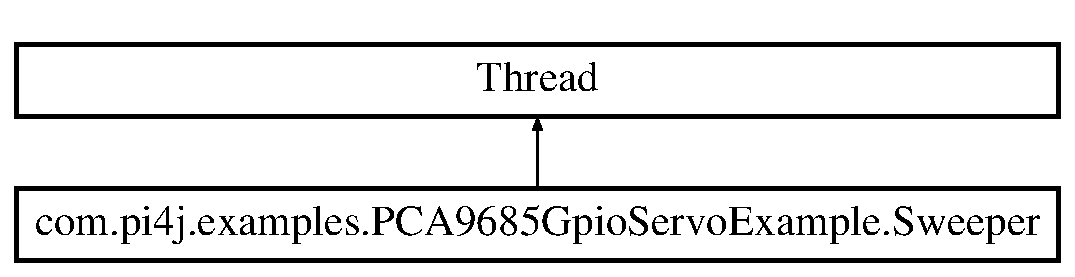
\includegraphics[height=2.000000cm]{classcom_1_1pi4j_1_1examples_1_1PCA9685GpioServoExample_1_1Sweeper}
\end{center}
\end{figure}
\subsection*{Public Member Functions}
\begin{DoxyCompactItemize}
\item 
void \hyperlink{classcom_1_1pi4j_1_1examples_1_1PCA9685GpioServoExample_1_1Sweeper_aa4e3dc19ea42e5fe72f0dbdcda223471}{run} ()
\item 
void \hyperlink{classcom_1_1pi4j_1_1examples_1_1PCA9685GpioServoExample_1_1Sweeper_a033c9258bceb96d71b5a6adfacb04976}{set\+Speed} (int \hyperlink{classcom_1_1pi4j_1_1examples_1_1PCA9685GpioServoExample_1_1Sweeper_a687365830c8cf1d68b44afc369bed00f}{speed})
\end{DoxyCompactItemize}
\subsection*{Private Attributes}
\begin{DoxyCompactItemize}
\item 
int \hyperlink{classcom_1_1pi4j_1_1examples_1_1PCA9685GpioServoExample_1_1Sweeper_a687365830c8cf1d68b44afc369bed00f}{speed} = 5
\end{DoxyCompactItemize}
\subsection*{Static Private Attributes}
\begin{DoxyCompactItemize}
\item 
static final int \hyperlink{classcom_1_1pi4j_1_1examples_1_1PCA9685GpioServoExample_1_1Sweeper_a5616b6c917a05769e3b3344710f6db3f}{S\+T\+E\+P} = 1
\item 
static final int \hyperlink{classcom_1_1pi4j_1_1examples_1_1PCA9685GpioServoExample_1_1Sweeper_a7643dfab6ffcfd44d60f83b03b507ab1}{M\+A\+X\+S\+L\+E\+E\+P\+B\+E\+T\+W\+E\+E\+N\+S\+T\+E\+P\+S} = 100
\end{DoxyCompactItemize}


\subsection{Member Function Documentation}
\hypertarget{classcom_1_1pi4j_1_1examples_1_1PCA9685GpioServoExample_1_1Sweeper_aa4e3dc19ea42e5fe72f0dbdcda223471}{}\index{com\+::pi4j\+::examples\+::\+P\+C\+A9685\+Gpio\+Servo\+Example\+::\+Sweeper@{com\+::pi4j\+::examples\+::\+P\+C\+A9685\+Gpio\+Servo\+Example\+::\+Sweeper}!run@{run}}
\index{run@{run}!com\+::pi4j\+::examples\+::\+P\+C\+A9685\+Gpio\+Servo\+Example\+::\+Sweeper@{com\+::pi4j\+::examples\+::\+P\+C\+A9685\+Gpio\+Servo\+Example\+::\+Sweeper}}
\subsubsection[{run}]{\setlength{\rightskip}{0pt plus 5cm}void com.\+pi4j.\+examples.\+P\+C\+A9685\+Gpio\+Servo\+Example.\+Sweeper.\+run (
\begin{DoxyParamCaption}
{}
\end{DoxyParamCaption}
)}\label{classcom_1_1pi4j_1_1examples_1_1PCA9685GpioServoExample_1_1Sweeper_aa4e3dc19ea42e5fe72f0dbdcda223471}
\hypertarget{classcom_1_1pi4j_1_1examples_1_1PCA9685GpioServoExample_1_1Sweeper_a033c9258bceb96d71b5a6adfacb04976}{}\index{com\+::pi4j\+::examples\+::\+P\+C\+A9685\+Gpio\+Servo\+Example\+::\+Sweeper@{com\+::pi4j\+::examples\+::\+P\+C\+A9685\+Gpio\+Servo\+Example\+::\+Sweeper}!set\+Speed@{set\+Speed}}
\index{set\+Speed@{set\+Speed}!com\+::pi4j\+::examples\+::\+P\+C\+A9685\+Gpio\+Servo\+Example\+::\+Sweeper@{com\+::pi4j\+::examples\+::\+P\+C\+A9685\+Gpio\+Servo\+Example\+::\+Sweeper}}
\subsubsection[{set\+Speed}]{\setlength{\rightskip}{0pt plus 5cm}void com.\+pi4j.\+examples.\+P\+C\+A9685\+Gpio\+Servo\+Example.\+Sweeper.\+set\+Speed (
\begin{DoxyParamCaption}
\item[{int}]{speed}
\end{DoxyParamCaption}
)}\label{classcom_1_1pi4j_1_1examples_1_1PCA9685GpioServoExample_1_1Sweeper_a033c9258bceb96d71b5a6adfacb04976}


\subsection{Member Data Documentation}
\hypertarget{classcom_1_1pi4j_1_1examples_1_1PCA9685GpioServoExample_1_1Sweeper_a7643dfab6ffcfd44d60f83b03b507ab1}{}\index{com\+::pi4j\+::examples\+::\+P\+C\+A9685\+Gpio\+Servo\+Example\+::\+Sweeper@{com\+::pi4j\+::examples\+::\+P\+C\+A9685\+Gpio\+Servo\+Example\+::\+Sweeper}!M\+A\+X\+S\+L\+E\+E\+P\+B\+E\+T\+W\+E\+E\+N\+S\+T\+E\+P\+S@{M\+A\+X\+S\+L\+E\+E\+P\+B\+E\+T\+W\+E\+E\+N\+S\+T\+E\+P\+S}}
\index{M\+A\+X\+S\+L\+E\+E\+P\+B\+E\+T\+W\+E\+E\+N\+S\+T\+E\+P\+S@{M\+A\+X\+S\+L\+E\+E\+P\+B\+E\+T\+W\+E\+E\+N\+S\+T\+E\+P\+S}!com\+::pi4j\+::examples\+::\+P\+C\+A9685\+Gpio\+Servo\+Example\+::\+Sweeper@{com\+::pi4j\+::examples\+::\+P\+C\+A9685\+Gpio\+Servo\+Example\+::\+Sweeper}}
\subsubsection[{M\+A\+X\+S\+L\+E\+E\+P\+B\+E\+T\+W\+E\+E\+N\+S\+T\+E\+P\+S}]{\setlength{\rightskip}{0pt plus 5cm}final int com.\+pi4j.\+examples.\+P\+C\+A9685\+Gpio\+Servo\+Example.\+Sweeper.\+M\+A\+X\+S\+L\+E\+E\+P\+B\+E\+T\+W\+E\+E\+N\+S\+T\+E\+P\+S = 100\hspace{0.3cm}{\ttfamily [static]}, {\ttfamily [private]}}\label{classcom_1_1pi4j_1_1examples_1_1PCA9685GpioServoExample_1_1Sweeper_a7643dfab6ffcfd44d60f83b03b507ab1}
\hypertarget{classcom_1_1pi4j_1_1examples_1_1PCA9685GpioServoExample_1_1Sweeper_a687365830c8cf1d68b44afc369bed00f}{}\index{com\+::pi4j\+::examples\+::\+P\+C\+A9685\+Gpio\+Servo\+Example\+::\+Sweeper@{com\+::pi4j\+::examples\+::\+P\+C\+A9685\+Gpio\+Servo\+Example\+::\+Sweeper}!speed@{speed}}
\index{speed@{speed}!com\+::pi4j\+::examples\+::\+P\+C\+A9685\+Gpio\+Servo\+Example\+::\+Sweeper@{com\+::pi4j\+::examples\+::\+P\+C\+A9685\+Gpio\+Servo\+Example\+::\+Sweeper}}
\subsubsection[{speed}]{\setlength{\rightskip}{0pt plus 5cm}int com.\+pi4j.\+examples.\+P\+C\+A9685\+Gpio\+Servo\+Example.\+Sweeper.\+speed = 5\hspace{0.3cm}{\ttfamily [private]}}\label{classcom_1_1pi4j_1_1examples_1_1PCA9685GpioServoExample_1_1Sweeper_a687365830c8cf1d68b44afc369bed00f}
\hypertarget{classcom_1_1pi4j_1_1examples_1_1PCA9685GpioServoExample_1_1Sweeper_a5616b6c917a05769e3b3344710f6db3f}{}\index{com\+::pi4j\+::examples\+::\+P\+C\+A9685\+Gpio\+Servo\+Example\+::\+Sweeper@{com\+::pi4j\+::examples\+::\+P\+C\+A9685\+Gpio\+Servo\+Example\+::\+Sweeper}!S\+T\+E\+P@{S\+T\+E\+P}}
\index{S\+T\+E\+P@{S\+T\+E\+P}!com\+::pi4j\+::examples\+::\+P\+C\+A9685\+Gpio\+Servo\+Example\+::\+Sweeper@{com\+::pi4j\+::examples\+::\+P\+C\+A9685\+Gpio\+Servo\+Example\+::\+Sweeper}}
\subsubsection[{S\+T\+E\+P}]{\setlength{\rightskip}{0pt plus 5cm}final int com.\+pi4j.\+examples.\+P\+C\+A9685\+Gpio\+Servo\+Example.\+Sweeper.\+S\+T\+E\+P = 1\hspace{0.3cm}{\ttfamily [static]}, {\ttfamily [private]}}\label{classcom_1_1pi4j_1_1examples_1_1PCA9685GpioServoExample_1_1Sweeper_a5616b6c917a05769e3b3344710f6db3f}


The documentation for this class was generated from the following file\+:\begin{DoxyCompactItemize}
\item 
main/java/com/pi4j/examples/\hyperlink{PCA9685GpioServoExample_8java}{P\+C\+A9685\+Gpio\+Servo\+Example.\+java}\end{DoxyCompactItemize}

\hypertarget{classcom_1_1pi4j_1_1examples_1_1SystemInfoExample}{}\section{com.\+pi4j.\+examples.\+System\+Info\+Example Class Reference}
\label{classcom_1_1pi4j_1_1examples_1_1SystemInfoExample}\index{com.\+pi4j.\+examples.\+System\+Info\+Example@{com.\+pi4j.\+examples.\+System\+Info\+Example}}
\subsection*{Static Public Member Functions}
\begin{DoxyCompactItemize}
\item 
static void \hyperlink{classcom_1_1pi4j_1_1examples_1_1SystemInfoExample_ae080b767ecc6c2e52b8567642a835a21}{main} (String\mbox{[}$\,$\mbox{]} args)  throws Interrupted\+Exception,             I\+O\+Exception, Parse\+Exception 
\end{DoxyCompactItemize}
\subsection*{Static Private Attributes}
\begin{DoxyCompactItemize}
\item 
static final Logger \hyperlink{classcom_1_1pi4j_1_1examples_1_1SystemInfoExample_ae8139fbdf213b0a34f5809c18d2d1693}{L\+O\+G\+G\+E\+R}
\item 
static final String \hyperlink{classcom_1_1pi4j_1_1examples_1_1SystemInfoExample_a81a12af5bdd93c15ca58b21a02a6d2ac}{T\+R\+A\+C\+E\+D\+\_\+\+L\+I\+N\+E} = \char`\"{}-\/-\/-\/-\/-\/-\/-\/-\/-\/-\/-\/-\/-\/-\/-\/-\/-\/-\/-\/-\/-\/-\/-\/-\/-\/-\/-\/-\/-\/-\/-\/-\/-\/-\/-\/-\/-\/-\/-\/-\/-\/-\/-\/-\/-\/-\/-\/-\/-\/-\/-\/-\/\char`\"{}
\end{DoxyCompactItemize}


\subsection{Detailed Description}
This example code demonstrates how to access a few of the system information properties and network information from the Raspberry Pi.

\begin{DoxyAuthor}{Author}
Robert Savage 
\end{DoxyAuthor}


\subsection{Member Function Documentation}
\hypertarget{classcom_1_1pi4j_1_1examples_1_1SystemInfoExample_ae080b767ecc6c2e52b8567642a835a21}{}\index{com\+::pi4j\+::examples\+::\+System\+Info\+Example@{com\+::pi4j\+::examples\+::\+System\+Info\+Example}!main@{main}}
\index{main@{main}!com\+::pi4j\+::examples\+::\+System\+Info\+Example@{com\+::pi4j\+::examples\+::\+System\+Info\+Example}}
\subsubsection[{main}]{\setlength{\rightskip}{0pt plus 5cm}static void com.\+pi4j.\+examples.\+System\+Info\+Example.\+main (
\begin{DoxyParamCaption}
\item[{String\mbox{[}$\,$\mbox{]}}]{args}
\end{DoxyParamCaption}
) throws Interrupted\+Exception,             I\+O\+Exception, Parse\+Exception\hspace{0.3cm}{\ttfamily [static]}}\label{classcom_1_1pi4j_1_1examples_1_1SystemInfoExample_ae080b767ecc6c2e52b8567642a835a21}


\subsection{Member Data Documentation}
\hypertarget{classcom_1_1pi4j_1_1examples_1_1SystemInfoExample_ae8139fbdf213b0a34f5809c18d2d1693}{}\index{com\+::pi4j\+::examples\+::\+System\+Info\+Example@{com\+::pi4j\+::examples\+::\+System\+Info\+Example}!L\+O\+G\+G\+E\+R@{L\+O\+G\+G\+E\+R}}
\index{L\+O\+G\+G\+E\+R@{L\+O\+G\+G\+E\+R}!com\+::pi4j\+::examples\+::\+System\+Info\+Example@{com\+::pi4j\+::examples\+::\+System\+Info\+Example}}
\subsubsection[{L\+O\+G\+G\+E\+R}]{\setlength{\rightskip}{0pt plus 5cm}final Logger com.\+pi4j.\+examples.\+System\+Info\+Example.\+L\+O\+G\+G\+E\+R\hspace{0.3cm}{\ttfamily [static]}, {\ttfamily [private]}}\label{classcom_1_1pi4j_1_1examples_1_1SystemInfoExample_ae8139fbdf213b0a34f5809c18d2d1693}
{\bfseries Initial value\+:}
\begin{DoxyCode}
= LogManager
            .getLogger(SystemInfoExample.class.getName())
\end{DoxyCode}
\hypertarget{classcom_1_1pi4j_1_1examples_1_1SystemInfoExample_a81a12af5bdd93c15ca58b21a02a6d2ac}{}\index{com\+::pi4j\+::examples\+::\+System\+Info\+Example@{com\+::pi4j\+::examples\+::\+System\+Info\+Example}!T\+R\+A\+C\+E\+D\+\_\+\+L\+I\+N\+E@{T\+R\+A\+C\+E\+D\+\_\+\+L\+I\+N\+E}}
\index{T\+R\+A\+C\+E\+D\+\_\+\+L\+I\+N\+E@{T\+R\+A\+C\+E\+D\+\_\+\+L\+I\+N\+E}!com\+::pi4j\+::examples\+::\+System\+Info\+Example@{com\+::pi4j\+::examples\+::\+System\+Info\+Example}}
\subsubsection[{T\+R\+A\+C\+E\+D\+\_\+\+L\+I\+N\+E}]{\setlength{\rightskip}{0pt plus 5cm}final String com.\+pi4j.\+examples.\+System\+Info\+Example.\+T\+R\+A\+C\+E\+D\+\_\+\+L\+I\+N\+E = \char`\"{}-\/-\/-\/-\/-\/-\/-\/-\/-\/-\/-\/-\/-\/-\/-\/-\/-\/-\/-\/-\/-\/-\/-\/-\/-\/-\/-\/-\/-\/-\/-\/-\/-\/-\/-\/-\/-\/-\/-\/-\/-\/-\/-\/-\/-\/-\/-\/-\/-\/-\/-\/-\/\char`\"{}\hspace{0.3cm}{\ttfamily [static]}, {\ttfamily [private]}}\label{classcom_1_1pi4j_1_1examples_1_1SystemInfoExample_a81a12af5bdd93c15ca58b21a02a6d2ac}


The documentation for this class was generated from the following file\+:\begin{DoxyCompactItemize}
\item 
main/java/com/pi4j/examples/\hyperlink{SystemInfoExample_8java}{System\+Info\+Example.\+java}\end{DoxyCompactItemize}

\hypertarget{classcom_1_1libsensorj_1_1concreteevent_1_1TemperatureEvent}{}\section{com.\+libsensorj.\+concreteevent.\+Temperature\+Event Class Reference}
\label{classcom_1_1libsensorj_1_1concreteevent_1_1TemperatureEvent}\index{com.\+libsensorj.\+concreteevent.\+Temperature\+Event@{com.\+libsensorj.\+concreteevent.\+Temperature\+Event}}
Inheritance diagram for com.\+libsensorj.\+concreteevent.\+Temperature\+Event\+:\begin{figure}[H]
\begin{center}
\leavevmode
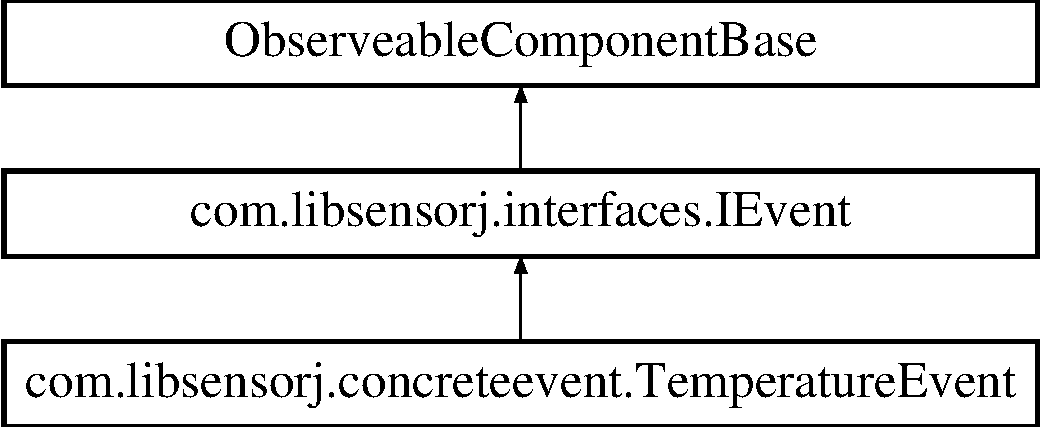
\includegraphics[height=3.000000cm]{classcom_1_1libsensorj_1_1concreteevent_1_1TemperatureEvent}
\end{center}
\end{figure}
\subsection*{Public Member Functions}
\begin{DoxyCompactItemize}
\item 
void \hyperlink{classcom_1_1libsensorj_1_1concreteevent_1_1TemperatureEvent_ad3499315aef403dfde60cf7d9a42c8cf}{attach} (\hyperlink{classcom_1_1libsensorj_1_1model_1_1Observer}{Observer} obsever)
\item 
void \hyperlink{classcom_1_1libsensorj_1_1concreteevent_1_1TemperatureEvent_a7332f144af23c349f39dd714de9c07b9}{detach} (\hyperlink{classcom_1_1libsensorj_1_1model_1_1Observer}{Observer} obsever)
\item 
void \hyperlink{classcom_1_1libsensorj_1_1concreteevent_1_1TemperatureEvent_ac0fe5a9964739808ece4fc9f2562dca5}{trigger} ()
\end{DoxyCompactItemize}


\subsection{Detailed Description}
The Class \hyperlink{classcom_1_1libsensorj_1_1concreteevent_1_1TemperatureEvent}{Temperature\+Event}. 

\subsection{Member Function Documentation}
\hypertarget{classcom_1_1libsensorj_1_1concreteevent_1_1TemperatureEvent_ad3499315aef403dfde60cf7d9a42c8cf}{}\index{com\+::libsensorj\+::concreteevent\+::\+Temperature\+Event@{com\+::libsensorj\+::concreteevent\+::\+Temperature\+Event}!attach@{attach}}
\index{attach@{attach}!com\+::libsensorj\+::concreteevent\+::\+Temperature\+Event@{com\+::libsensorj\+::concreteevent\+::\+Temperature\+Event}}
\subsubsection[{attach}]{\setlength{\rightskip}{0pt plus 5cm}void com.\+libsensorj.\+concreteevent.\+Temperature\+Event.\+attach (
\begin{DoxyParamCaption}
\item[{{\bf Observer}}]{obsever}
\end{DoxyParamCaption}
)}\label{classcom_1_1libsensorj_1_1concreteevent_1_1TemperatureEvent_ad3499315aef403dfde60cf7d9a42c8cf}
\hypertarget{classcom_1_1libsensorj_1_1concreteevent_1_1TemperatureEvent_a7332f144af23c349f39dd714de9c07b9}{}\index{com\+::libsensorj\+::concreteevent\+::\+Temperature\+Event@{com\+::libsensorj\+::concreteevent\+::\+Temperature\+Event}!detach@{detach}}
\index{detach@{detach}!com\+::libsensorj\+::concreteevent\+::\+Temperature\+Event@{com\+::libsensorj\+::concreteevent\+::\+Temperature\+Event}}
\subsubsection[{detach}]{\setlength{\rightskip}{0pt plus 5cm}void com.\+libsensorj.\+concreteevent.\+Temperature\+Event.\+detach (
\begin{DoxyParamCaption}
\item[{{\bf Observer}}]{obsever}
\end{DoxyParamCaption}
)}\label{classcom_1_1libsensorj_1_1concreteevent_1_1TemperatureEvent_a7332f144af23c349f39dd714de9c07b9}
\hypertarget{classcom_1_1libsensorj_1_1concreteevent_1_1TemperatureEvent_ac0fe5a9964739808ece4fc9f2562dca5}{}\index{com\+::libsensorj\+::concreteevent\+::\+Temperature\+Event@{com\+::libsensorj\+::concreteevent\+::\+Temperature\+Event}!trigger@{trigger}}
\index{trigger@{trigger}!com\+::libsensorj\+::concreteevent\+::\+Temperature\+Event@{com\+::libsensorj\+::concreteevent\+::\+Temperature\+Event}}
\subsubsection[{trigger}]{\setlength{\rightskip}{0pt plus 5cm}void com.\+libsensorj.\+concreteevent.\+Temperature\+Event.\+trigger (
\begin{DoxyParamCaption}
{}
\end{DoxyParamCaption}
)}\label{classcom_1_1libsensorj_1_1concreteevent_1_1TemperatureEvent_ac0fe5a9964739808ece4fc9f2562dca5}


The documentation for this class was generated from the following file\+:\begin{DoxyCompactItemize}
\item 
main/java/com/libsensorj/concreteevent/\hyperlink{TemperatureEvent_8java}{Temperature\+Event.\+java}\end{DoxyCompactItemize}

\hypertarget{classcom_1_1libsensorj_1_1concretefactory_1_1TemperatureSensorFactory}{}\section{com.\+libsensorj.\+concretefactory.\+Temperature\+Sensor\+Factory Class Reference}
\label{classcom_1_1libsensorj_1_1concretefactory_1_1TemperatureSensorFactory}\index{com.\+libsensorj.\+concretefactory.\+Temperature\+Sensor\+Factory@{com.\+libsensorj.\+concretefactory.\+Temperature\+Sensor\+Factory}}
Inheritance diagram for com.\+libsensorj.\+concretefactory.\+Temperature\+Sensor\+Factory\+:\begin{figure}[H]
\begin{center}
\leavevmode
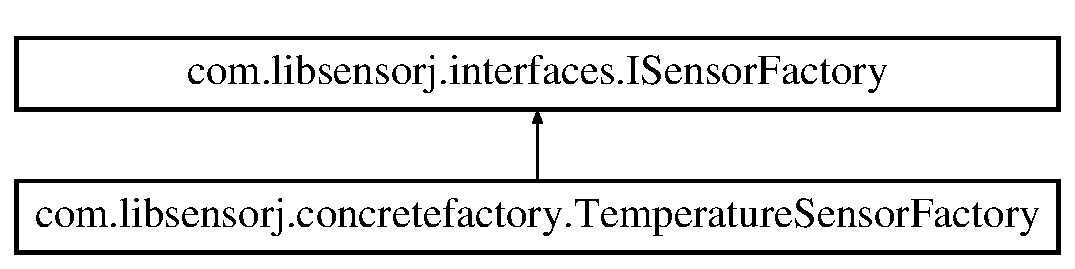
\includegraphics[height=2.000000cm]{classcom_1_1libsensorj_1_1concretefactory_1_1TemperatureSensorFactory}
\end{center}
\end{figure}
\subsection*{Public Member Functions}
\begin{DoxyCompactItemize}
\item 
\hyperlink{interfacecom_1_1libsensorj_1_1interfaces_1_1ISensor}{I\+Sensor} \hyperlink{classcom_1_1libsensorj_1_1concretefactory_1_1TemperatureSensorFactory_aeba8598ebe5c182154f63e0c94abdd70}{create\+Sensor} ()
\item 
\hyperlink{interfacecom_1_1libsensorj_1_1interfaces_1_1IEvent}{I\+Event} \hyperlink{classcom_1_1libsensorj_1_1concretefactory_1_1TemperatureSensorFactory_adb3d5716b5e55f4fc037c0a95ec99688}{create\+Event} ()
\end{DoxyCompactItemize}


\subsection{Member Function Documentation}
\hypertarget{classcom_1_1libsensorj_1_1concretefactory_1_1TemperatureSensorFactory_adb3d5716b5e55f4fc037c0a95ec99688}{}\index{com\+::libsensorj\+::concretefactory\+::\+Temperature\+Sensor\+Factory@{com\+::libsensorj\+::concretefactory\+::\+Temperature\+Sensor\+Factory}!create\+Event@{create\+Event}}
\index{create\+Event@{create\+Event}!com\+::libsensorj\+::concretefactory\+::\+Temperature\+Sensor\+Factory@{com\+::libsensorj\+::concretefactory\+::\+Temperature\+Sensor\+Factory}}
\subsubsection[{create\+Event}]{\setlength{\rightskip}{0pt plus 5cm}{\bf I\+Event} com.\+libsensorj.\+concretefactory.\+Temperature\+Sensor\+Factory.\+create\+Event (
\begin{DoxyParamCaption}
{}
\end{DoxyParamCaption}
)}\label{classcom_1_1libsensorj_1_1concretefactory_1_1TemperatureSensorFactory_adb3d5716b5e55f4fc037c0a95ec99688}


Implements \hyperlink{interfacecom_1_1libsensorj_1_1interfaces_1_1ISensorFactory_a2b074d01287a4e64677097255ba9e768}{com.\+libsensorj.\+interfaces.\+I\+Sensor\+Factory}.

\hypertarget{classcom_1_1libsensorj_1_1concretefactory_1_1TemperatureSensorFactory_aeba8598ebe5c182154f63e0c94abdd70}{}\index{com\+::libsensorj\+::concretefactory\+::\+Temperature\+Sensor\+Factory@{com\+::libsensorj\+::concretefactory\+::\+Temperature\+Sensor\+Factory}!create\+Sensor@{create\+Sensor}}
\index{create\+Sensor@{create\+Sensor}!com\+::libsensorj\+::concretefactory\+::\+Temperature\+Sensor\+Factory@{com\+::libsensorj\+::concretefactory\+::\+Temperature\+Sensor\+Factory}}
\subsubsection[{create\+Sensor}]{\setlength{\rightskip}{0pt plus 5cm}{\bf I\+Sensor} com.\+libsensorj.\+concretefactory.\+Temperature\+Sensor\+Factory.\+create\+Sensor (
\begin{DoxyParamCaption}
{}
\end{DoxyParamCaption}
)}\label{classcom_1_1libsensorj_1_1concretefactory_1_1TemperatureSensorFactory_aeba8598ebe5c182154f63e0c94abdd70}


Implements \hyperlink{interfacecom_1_1libsensorj_1_1interfaces_1_1ISensorFactory_ac14c6d566c37c6a79c6db1e85634f25d}{com.\+libsensorj.\+interfaces.\+I\+Sensor\+Factory}.



The documentation for this class was generated from the following file\+:\begin{DoxyCompactItemize}
\item 
main/java/com/libsensorj/concretefactory/\hyperlink{TemperatureSensorFactory_8java}{Temperature\+Sensor\+Factory.\+java}\end{DoxyCompactItemize}

\hypertarget{classcom_1_1pi4j_1_1examples_1_1I2CWiiMotionPlusExample_1_1ThreeAxis}{}\section{com.\+pi4j.\+examples.\+I2\+C\+Wii\+Motion\+Plus\+Example.\+Three\+Axis Class Reference}
\label{classcom_1_1pi4j_1_1examples_1_1I2CWiiMotionPlusExample_1_1ThreeAxis}\index{com.\+pi4j.\+examples.\+I2\+C\+Wii\+Motion\+Plus\+Example.\+Three\+Axis@{com.\+pi4j.\+examples.\+I2\+C\+Wii\+Motion\+Plus\+Example.\+Three\+Axis}}
\subsection*{Public Attributes}
\begin{DoxyCompactItemize}
\item 
int \hyperlink{classcom_1_1pi4j_1_1examples_1_1I2CWiiMotionPlusExample_1_1ThreeAxis_a50f255ff981b2b2d64301a7439bf07ba}{x}
\item 
int \hyperlink{classcom_1_1pi4j_1_1examples_1_1I2CWiiMotionPlusExample_1_1ThreeAxis_a271c8a23d3b08a697207aeabbb4fc523}{y}
\item 
int \hyperlink{classcom_1_1pi4j_1_1examples_1_1I2CWiiMotionPlusExample_1_1ThreeAxis_a49d88e91188af7cc75cb642be222ebd9}{z}
\end{DoxyCompactItemize}


\subsection{Member Data Documentation}
\hypertarget{classcom_1_1pi4j_1_1examples_1_1I2CWiiMotionPlusExample_1_1ThreeAxis_a50f255ff981b2b2d64301a7439bf07ba}{}\index{com\+::pi4j\+::examples\+::\+I2\+C\+Wii\+Motion\+Plus\+Example\+::\+Three\+Axis@{com\+::pi4j\+::examples\+::\+I2\+C\+Wii\+Motion\+Plus\+Example\+::\+Three\+Axis}!x@{x}}
\index{x@{x}!com\+::pi4j\+::examples\+::\+I2\+C\+Wii\+Motion\+Plus\+Example\+::\+Three\+Axis@{com\+::pi4j\+::examples\+::\+I2\+C\+Wii\+Motion\+Plus\+Example\+::\+Three\+Axis}}
\subsubsection[{x}]{\setlength{\rightskip}{0pt plus 5cm}int com.\+pi4j.\+examples.\+I2\+C\+Wii\+Motion\+Plus\+Example.\+Three\+Axis.\+x}\label{classcom_1_1pi4j_1_1examples_1_1I2CWiiMotionPlusExample_1_1ThreeAxis_a50f255ff981b2b2d64301a7439bf07ba}
\hypertarget{classcom_1_1pi4j_1_1examples_1_1I2CWiiMotionPlusExample_1_1ThreeAxis_a271c8a23d3b08a697207aeabbb4fc523}{}\index{com\+::pi4j\+::examples\+::\+I2\+C\+Wii\+Motion\+Plus\+Example\+::\+Three\+Axis@{com\+::pi4j\+::examples\+::\+I2\+C\+Wii\+Motion\+Plus\+Example\+::\+Three\+Axis}!y@{y}}
\index{y@{y}!com\+::pi4j\+::examples\+::\+I2\+C\+Wii\+Motion\+Plus\+Example\+::\+Three\+Axis@{com\+::pi4j\+::examples\+::\+I2\+C\+Wii\+Motion\+Plus\+Example\+::\+Three\+Axis}}
\subsubsection[{y}]{\setlength{\rightskip}{0pt plus 5cm}int com.\+pi4j.\+examples.\+I2\+C\+Wii\+Motion\+Plus\+Example.\+Three\+Axis.\+y}\label{classcom_1_1pi4j_1_1examples_1_1I2CWiiMotionPlusExample_1_1ThreeAxis_a271c8a23d3b08a697207aeabbb4fc523}
\hypertarget{classcom_1_1pi4j_1_1examples_1_1I2CWiiMotionPlusExample_1_1ThreeAxis_a49d88e91188af7cc75cb642be222ebd9}{}\index{com\+::pi4j\+::examples\+::\+I2\+C\+Wii\+Motion\+Plus\+Example\+::\+Three\+Axis@{com\+::pi4j\+::examples\+::\+I2\+C\+Wii\+Motion\+Plus\+Example\+::\+Three\+Axis}!z@{z}}
\index{z@{z}!com\+::pi4j\+::examples\+::\+I2\+C\+Wii\+Motion\+Plus\+Example\+::\+Three\+Axis@{com\+::pi4j\+::examples\+::\+I2\+C\+Wii\+Motion\+Plus\+Example\+::\+Three\+Axis}}
\subsubsection[{z}]{\setlength{\rightskip}{0pt plus 5cm}int com.\+pi4j.\+examples.\+I2\+C\+Wii\+Motion\+Plus\+Example.\+Three\+Axis.\+z}\label{classcom_1_1pi4j_1_1examples_1_1I2CWiiMotionPlusExample_1_1ThreeAxis_a49d88e91188af7cc75cb642be222ebd9}


The documentation for this class was generated from the following file\+:\begin{DoxyCompactItemize}
\item 
main/java/com/pi4j/examples/\hyperlink{I2CWiiMotionPlusExample_8java}{I2\+C\+Wii\+Motion\+Plus\+Example.\+java}\end{DoxyCompactItemize}

\hypertarget{classcom_1_1pi4j_1_1examples_1_1TriggerGpioExample}{}\section{com.\+pi4j.\+examples.\+Trigger\+Gpio\+Example Class Reference}
\label{classcom_1_1pi4j_1_1examples_1_1TriggerGpioExample}\index{com.\+pi4j.\+examples.\+Trigger\+Gpio\+Example@{com.\+pi4j.\+examples.\+Trigger\+Gpio\+Example}}
\subsection*{Static Public Member Functions}
\begin{DoxyCompactItemize}
\item 
static void \hyperlink{classcom_1_1pi4j_1_1examples_1_1TriggerGpioExample_ad286827e1917615f5f1ec8170f17d114}{main} (String\mbox{[}$\,$\mbox{]} args)  throws Interrupted\+Exception 
\end{DoxyCompactItemize}
\subsection*{Static Private Attributes}
\begin{DoxyCompactItemize}
\item 
static final Logger \hyperlink{classcom_1_1pi4j_1_1examples_1_1TriggerGpioExample_ab2cd00493648e1d0e4e7d6c42be75449}{L\+O\+G\+G\+E\+R}
\end{DoxyCompactItemize}


\subsection{Detailed Description}
This example code demonstrates how to setup simple triggers for G\+P\+I\+O pins on the Raspberry Pi.

\begin{DoxyAuthor}{Author}
Robert Savage 
\end{DoxyAuthor}


\subsection{Member Function Documentation}
\hypertarget{classcom_1_1pi4j_1_1examples_1_1TriggerGpioExample_ad286827e1917615f5f1ec8170f17d114}{}\index{com\+::pi4j\+::examples\+::\+Trigger\+Gpio\+Example@{com\+::pi4j\+::examples\+::\+Trigger\+Gpio\+Example}!main@{main}}
\index{main@{main}!com\+::pi4j\+::examples\+::\+Trigger\+Gpio\+Example@{com\+::pi4j\+::examples\+::\+Trigger\+Gpio\+Example}}
\subsubsection[{main}]{\setlength{\rightskip}{0pt plus 5cm}static void com.\+pi4j.\+examples.\+Trigger\+Gpio\+Example.\+main (
\begin{DoxyParamCaption}
\item[{String\mbox{[}$\,$\mbox{]}}]{args}
\end{DoxyParamCaption}
) throws Interrupted\+Exception\hspace{0.3cm}{\ttfamily [static]}}\label{classcom_1_1pi4j_1_1examples_1_1TriggerGpioExample_ad286827e1917615f5f1ec8170f17d114}


\subsection{Member Data Documentation}
\hypertarget{classcom_1_1pi4j_1_1examples_1_1TriggerGpioExample_ab2cd00493648e1d0e4e7d6c42be75449}{}\index{com\+::pi4j\+::examples\+::\+Trigger\+Gpio\+Example@{com\+::pi4j\+::examples\+::\+Trigger\+Gpio\+Example}!L\+O\+G\+G\+E\+R@{L\+O\+G\+G\+E\+R}}
\index{L\+O\+G\+G\+E\+R@{L\+O\+G\+G\+E\+R}!com\+::pi4j\+::examples\+::\+Trigger\+Gpio\+Example@{com\+::pi4j\+::examples\+::\+Trigger\+Gpio\+Example}}
\subsubsection[{L\+O\+G\+G\+E\+R}]{\setlength{\rightskip}{0pt plus 5cm}final Logger com.\+pi4j.\+examples.\+Trigger\+Gpio\+Example.\+L\+O\+G\+G\+E\+R\hspace{0.3cm}{\ttfamily [static]}, {\ttfamily [private]}}\label{classcom_1_1pi4j_1_1examples_1_1TriggerGpioExample_ab2cd00493648e1d0e4e7d6c42be75449}
{\bfseries Initial value\+:}
\begin{DoxyCode}
= LogManager
            .getLogger(TriggerGpioExample.class.getName())
\end{DoxyCode}


The documentation for this class was generated from the following file\+:\begin{DoxyCompactItemize}
\item 
main/java/com/pi4j/examples/\hyperlink{TriggerGpioExample_8java}{Trigger\+Gpio\+Example.\+java}\end{DoxyCompactItemize}

\hypertarget{classcom_1_1libsensorj_1_1concretesensor_1_1UltrasonicHcsr04}{}\section{com.\+libsensorj.\+concretesensor.\+Ultrasonic\+Hcsr04 Class Reference}
\label{classcom_1_1libsensorj_1_1concretesensor_1_1UltrasonicHcsr04}\index{com.\+libsensorj.\+concretesensor.\+Ultrasonic\+Hcsr04@{com.\+libsensorj.\+concretesensor.\+Ultrasonic\+Hcsr04}}
Inheritance diagram for com.\+libsensorj.\+concretesensor.\+Ultrasonic\+Hcsr04\+:\begin{figure}[H]
\begin{center}
\leavevmode
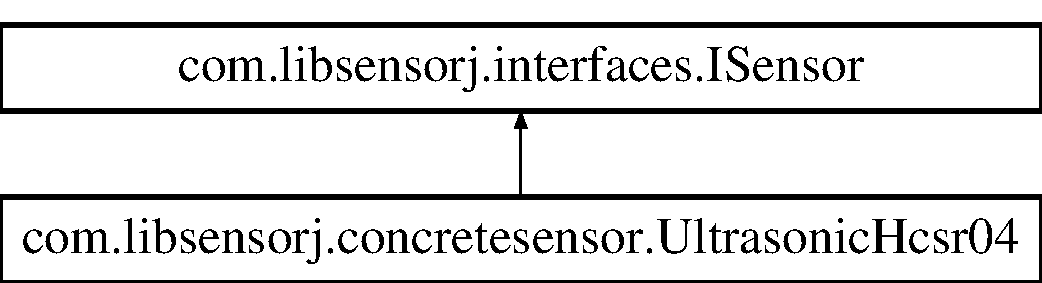
\includegraphics[height=2.000000cm]{classcom_1_1libsensorj_1_1concretesensor_1_1UltrasonicHcsr04}
\end{center}
\end{figure}
\subsection*{Public Member Functions}
\begin{DoxyCompactItemize}
\item 
\hyperlink{classcom_1_1libsensorj_1_1concretesensor_1_1UltrasonicHcsr04_a7e02068d9acb1b3cf1d15d45afbf377b}{Ultrasonic\+Hcsr04} ()
\item 
\hyperlink{classcom_1_1libsensorj_1_1concretesensor_1_1UltrasonicHcsr04_a14e708bf4eb89a2ceb0037fcb837522c}{Ultrasonic\+Hcsr04} (int \hyperlink{classcom_1_1libsensorj_1_1concretesensor_1_1UltrasonicHcsr04_a13705a8251de22d0f52caa3e17d23376}{trigger}, int \hyperlink{classcom_1_1libsensorj_1_1concretesensor_1_1UltrasonicHcsr04_a3695a560e3157a5e6f7896532d717456}{echo})
\item 
\hyperlink{classcom_1_1libsensorj_1_1concretesensor_1_1UltrasonicHcsr04_ae00a91eaf7e5c08695c50a670698ed5f}{Ultrasonic\+Hcsr04} (Pin \hyperlink{classcom_1_1libsensorj_1_1concretesensor_1_1UltrasonicHcsr04_a13705a8251de22d0f52caa3e17d23376}{trigger}, Pin \hyperlink{classcom_1_1libsensorj_1_1concretesensor_1_1UltrasonicHcsr04_a3695a560e3157a5e6f7896532d717456}{echo})
\item 
void \hyperlink{classcom_1_1libsensorj_1_1concretesensor_1_1UltrasonicHcsr04_a170167614b330d79518647a9a9722b62}{get\+Instance} ()
\item 
double \hyperlink{classcom_1_1libsensorj_1_1concretesensor_1_1UltrasonicHcsr04_aec68f4aadd8faa618025dfa37c89c696}{get\+Range} ()
\end{DoxyCompactItemize}
\subsection*{Private Attributes}
\begin{DoxyCompactItemize}
\item 
double \hyperlink{classcom_1_1libsensorj_1_1concretesensor_1_1UltrasonicHcsr04_aad32f417f9106fa8f3f2e2a7416f033b}{result} = 0
\item 
Gpio\+Pin\+Digital\+Output \hyperlink{classcom_1_1libsensorj_1_1concretesensor_1_1UltrasonicHcsr04_a13705a8251de22d0f52caa3e17d23376}{trigger}
\item 
Gpio\+Pin\+Digital\+Input \hyperlink{classcom_1_1libsensorj_1_1concretesensor_1_1UltrasonicHcsr04_a3695a560e3157a5e6f7896532d717456}{echo}
\end{DoxyCompactItemize}
\subsection*{Static Private Attributes}
\begin{DoxyCompactItemize}
\item 
static final int \hyperlink{classcom_1_1libsensorj_1_1concretesensor_1_1UltrasonicHcsr04_aa04a319fc4ef2ccf8de8a70bf27da2da}{T\+W\+E\+N\+T\+Y} = 20
\item 
static final int \hyperlink{classcom_1_1libsensorj_1_1concretesensor_1_1UltrasonicHcsr04_a7106eaa9f89d876a4749d502232964df}{F\+O\+R\+T\+Y} = 40
\item 
static final int \hyperlink{classcom_1_1libsensorj_1_1concretesensor_1_1UltrasonicHcsr04_a25452283296d3780a7fefbfa20e40a93}{T\+H\+I\+R\+T\+Y\+\_\+\+E\+I\+G\+H\+T} = 38
\item 
static final double \hyperlink{classcom_1_1libsensorj_1_1concretesensor_1_1UltrasonicHcsr04_a0483c4e470b1ab9e1a437fbeec6595e9}{D\+I\+S\+T\+A\+N\+C\+E\+\_\+\+F\+A\+C\+T\+O\+R} = 165.\+7
\item 
static final Logger \hyperlink{classcom_1_1libsensorj_1_1concretesensor_1_1UltrasonicHcsr04_a9a3534d952f2668b69b0888b9e929abb}{L\+O\+G\+G\+E\+R}
\end{DoxyCompactItemize}


\subsection{Detailed Description}
The Class \hyperlink{classcom_1_1libsensorj_1_1concretesensor_1_1UltrasonicHcsr04}{Ultrasonic\+Hcsr04}. 

\subsection{Constructor \& Destructor Documentation}
\hypertarget{classcom_1_1libsensorj_1_1concretesensor_1_1UltrasonicHcsr04_a7e02068d9acb1b3cf1d15d45afbf377b}{}\index{com\+::libsensorj\+::concretesensor\+::\+Ultrasonic\+Hcsr04@{com\+::libsensorj\+::concretesensor\+::\+Ultrasonic\+Hcsr04}!Ultrasonic\+Hcsr04@{Ultrasonic\+Hcsr04}}
\index{Ultrasonic\+Hcsr04@{Ultrasonic\+Hcsr04}!com\+::libsensorj\+::concretesensor\+::\+Ultrasonic\+Hcsr04@{com\+::libsensorj\+::concretesensor\+::\+Ultrasonic\+Hcsr04}}
\subsubsection[{Ultrasonic\+Hcsr04}]{\setlength{\rightskip}{0pt plus 5cm}com.\+libsensorj.\+concretesensor.\+Ultrasonic\+Hcsr04.\+Ultrasonic\+Hcsr04 (
\begin{DoxyParamCaption}
{}
\end{DoxyParamCaption}
)}\label{classcom_1_1libsensorj_1_1concretesensor_1_1UltrasonicHcsr04_a7e02068d9acb1b3cf1d15d45afbf377b}
Instantiates a new ultrasonic hcsr04. \hypertarget{classcom_1_1libsensorj_1_1concretesensor_1_1UltrasonicHcsr04_a14e708bf4eb89a2ceb0037fcb837522c}{}\index{com\+::libsensorj\+::concretesensor\+::\+Ultrasonic\+Hcsr04@{com\+::libsensorj\+::concretesensor\+::\+Ultrasonic\+Hcsr04}!Ultrasonic\+Hcsr04@{Ultrasonic\+Hcsr04}}
\index{Ultrasonic\+Hcsr04@{Ultrasonic\+Hcsr04}!com\+::libsensorj\+::concretesensor\+::\+Ultrasonic\+Hcsr04@{com\+::libsensorj\+::concretesensor\+::\+Ultrasonic\+Hcsr04}}
\subsubsection[{Ultrasonic\+Hcsr04}]{\setlength{\rightskip}{0pt plus 5cm}com.\+libsensorj.\+concretesensor.\+Ultrasonic\+Hcsr04.\+Ultrasonic\+Hcsr04 (
\begin{DoxyParamCaption}
\item[{int}]{trigger, }
\item[{int}]{echo}
\end{DoxyParamCaption}
)}\label{classcom_1_1libsensorj_1_1concretesensor_1_1UltrasonicHcsr04_a14e708bf4eb89a2ceb0037fcb837522c}
Instantiates a new ultrasonic hcsr04.


\begin{DoxyParams}{Parameters}
{\em trigger} & the trigger pin \\
\hline
{\em echo} & the echo pin \\
\hline
\end{DoxyParams}
\hypertarget{classcom_1_1libsensorj_1_1concretesensor_1_1UltrasonicHcsr04_ae00a91eaf7e5c08695c50a670698ed5f}{}\index{com\+::libsensorj\+::concretesensor\+::\+Ultrasonic\+Hcsr04@{com\+::libsensorj\+::concretesensor\+::\+Ultrasonic\+Hcsr04}!Ultrasonic\+Hcsr04@{Ultrasonic\+Hcsr04}}
\index{Ultrasonic\+Hcsr04@{Ultrasonic\+Hcsr04}!com\+::libsensorj\+::concretesensor\+::\+Ultrasonic\+Hcsr04@{com\+::libsensorj\+::concretesensor\+::\+Ultrasonic\+Hcsr04}}
\subsubsection[{Ultrasonic\+Hcsr04}]{\setlength{\rightskip}{0pt plus 5cm}com.\+libsensorj.\+concretesensor.\+Ultrasonic\+Hcsr04.\+Ultrasonic\+Hcsr04 (
\begin{DoxyParamCaption}
\item[{Pin}]{trigger, }
\item[{Pin}]{echo}
\end{DoxyParamCaption}
)}\label{classcom_1_1libsensorj_1_1concretesensor_1_1UltrasonicHcsr04_ae00a91eaf7e5c08695c50a670698ed5f}
Instantiates a new ultrasonic hcsr04.


\begin{DoxyParams}{Parameters}
{\em \+\_\+trigger} & the trigger pin \\
\hline
{\em \+\_\+echo} & the echo pin \\
\hline
\end{DoxyParams}


\subsection{Member Function Documentation}
\hypertarget{classcom_1_1libsensorj_1_1concretesensor_1_1UltrasonicHcsr04_a170167614b330d79518647a9a9722b62}{}\index{com\+::libsensorj\+::concretesensor\+::\+Ultrasonic\+Hcsr04@{com\+::libsensorj\+::concretesensor\+::\+Ultrasonic\+Hcsr04}!get\+Instance@{get\+Instance}}
\index{get\+Instance@{get\+Instance}!com\+::libsensorj\+::concretesensor\+::\+Ultrasonic\+Hcsr04@{com\+::libsensorj\+::concretesensor\+::\+Ultrasonic\+Hcsr04}}
\subsubsection[{get\+Instance}]{\setlength{\rightskip}{0pt plus 5cm}void com.\+libsensorj.\+concretesensor.\+Ultrasonic\+Hcsr04.\+get\+Instance (
\begin{DoxyParamCaption}
{}
\end{DoxyParamCaption}
)}\label{classcom_1_1libsensorj_1_1concretesensor_1_1UltrasonicHcsr04_a170167614b330d79518647a9a9722b62}
Gets the single instance of I\+Sensor.

\begin{DoxyReturn}{Returns}
single instance of I\+Sensor 
\end{DoxyReturn}


Implements \hyperlink{interfacecom_1_1libsensorj_1_1interfaces_1_1ISensor_a3c3db93a33adecde81a528651790f75e}{com.\+libsensorj.\+interfaces.\+I\+Sensor}.

\hypertarget{classcom_1_1libsensorj_1_1concretesensor_1_1UltrasonicHcsr04_aec68f4aadd8faa618025dfa37c89c696}{}\index{com\+::libsensorj\+::concretesensor\+::\+Ultrasonic\+Hcsr04@{com\+::libsensorj\+::concretesensor\+::\+Ultrasonic\+Hcsr04}!get\+Range@{get\+Range}}
\index{get\+Range@{get\+Range}!com\+::libsensorj\+::concretesensor\+::\+Ultrasonic\+Hcsr04@{com\+::libsensorj\+::concretesensor\+::\+Ultrasonic\+Hcsr04}}
\subsubsection[{get\+Range}]{\setlength{\rightskip}{0pt plus 5cm}double com.\+libsensorj.\+concretesensor.\+Ultrasonic\+Hcsr04.\+get\+Range (
\begin{DoxyParamCaption}
{}
\end{DoxyParamCaption}
)}\label{classcom_1_1libsensorj_1_1concretesensor_1_1UltrasonicHcsr04_aec68f4aadd8faa618025dfa37c89c696}
Gets the range.

\begin{DoxyReturn}{Returns}
the range 
\end{DoxyReturn}


\subsection{Member Data Documentation}
\hypertarget{classcom_1_1libsensorj_1_1concretesensor_1_1UltrasonicHcsr04_a0483c4e470b1ab9e1a437fbeec6595e9}{}\index{com\+::libsensorj\+::concretesensor\+::\+Ultrasonic\+Hcsr04@{com\+::libsensorj\+::concretesensor\+::\+Ultrasonic\+Hcsr04}!D\+I\+S\+T\+A\+N\+C\+E\+\_\+\+F\+A\+C\+T\+O\+R@{D\+I\+S\+T\+A\+N\+C\+E\+\_\+\+F\+A\+C\+T\+O\+R}}
\index{D\+I\+S\+T\+A\+N\+C\+E\+\_\+\+F\+A\+C\+T\+O\+R@{D\+I\+S\+T\+A\+N\+C\+E\+\_\+\+F\+A\+C\+T\+O\+R}!com\+::libsensorj\+::concretesensor\+::\+Ultrasonic\+Hcsr04@{com\+::libsensorj\+::concretesensor\+::\+Ultrasonic\+Hcsr04}}
\subsubsection[{D\+I\+S\+T\+A\+N\+C\+E\+\_\+\+F\+A\+C\+T\+O\+R}]{\setlength{\rightskip}{0pt plus 5cm}final double com.\+libsensorj.\+concretesensor.\+Ultrasonic\+Hcsr04.\+D\+I\+S\+T\+A\+N\+C\+E\+\_\+\+F\+A\+C\+T\+O\+R = 165.\+7\hspace{0.3cm}{\ttfamily [static]}, {\ttfamily [private]}}\label{classcom_1_1libsensorj_1_1concretesensor_1_1UltrasonicHcsr04_a0483c4e470b1ab9e1a437fbeec6595e9}
The Constant D\+I\+S\+T\+A\+N\+C\+E\+\_\+\+F\+A\+C\+T\+O\+R. \hypertarget{classcom_1_1libsensorj_1_1concretesensor_1_1UltrasonicHcsr04_a3695a560e3157a5e6f7896532d717456}{}\index{com\+::libsensorj\+::concretesensor\+::\+Ultrasonic\+Hcsr04@{com\+::libsensorj\+::concretesensor\+::\+Ultrasonic\+Hcsr04}!echo@{echo}}
\index{echo@{echo}!com\+::libsensorj\+::concretesensor\+::\+Ultrasonic\+Hcsr04@{com\+::libsensorj\+::concretesensor\+::\+Ultrasonic\+Hcsr04}}
\subsubsection[{echo}]{\setlength{\rightskip}{0pt plus 5cm}Gpio\+Pin\+Digital\+Input com.\+libsensorj.\+concretesensor.\+Ultrasonic\+Hcsr04.\+echo\hspace{0.3cm}{\ttfamily [private]}}\label{classcom_1_1libsensorj_1_1concretesensor_1_1UltrasonicHcsr04_a3695a560e3157a5e6f7896532d717456}
The echo. \hypertarget{classcom_1_1libsensorj_1_1concretesensor_1_1UltrasonicHcsr04_a7106eaa9f89d876a4749d502232964df}{}\index{com\+::libsensorj\+::concretesensor\+::\+Ultrasonic\+Hcsr04@{com\+::libsensorj\+::concretesensor\+::\+Ultrasonic\+Hcsr04}!F\+O\+R\+T\+Y@{F\+O\+R\+T\+Y}}
\index{F\+O\+R\+T\+Y@{F\+O\+R\+T\+Y}!com\+::libsensorj\+::concretesensor\+::\+Ultrasonic\+Hcsr04@{com\+::libsensorj\+::concretesensor\+::\+Ultrasonic\+Hcsr04}}
\subsubsection[{F\+O\+R\+T\+Y}]{\setlength{\rightskip}{0pt plus 5cm}final int com.\+libsensorj.\+concretesensor.\+Ultrasonic\+Hcsr04.\+F\+O\+R\+T\+Y = 40\hspace{0.3cm}{\ttfamily [static]}, {\ttfamily [private]}}\label{classcom_1_1libsensorj_1_1concretesensor_1_1UltrasonicHcsr04_a7106eaa9f89d876a4749d502232964df}
The Constant F\+O\+R\+T\+Y. \hypertarget{classcom_1_1libsensorj_1_1concretesensor_1_1UltrasonicHcsr04_a9a3534d952f2668b69b0888b9e929abb}{}\index{com\+::libsensorj\+::concretesensor\+::\+Ultrasonic\+Hcsr04@{com\+::libsensorj\+::concretesensor\+::\+Ultrasonic\+Hcsr04}!L\+O\+G\+G\+E\+R@{L\+O\+G\+G\+E\+R}}
\index{L\+O\+G\+G\+E\+R@{L\+O\+G\+G\+E\+R}!com\+::libsensorj\+::concretesensor\+::\+Ultrasonic\+Hcsr04@{com\+::libsensorj\+::concretesensor\+::\+Ultrasonic\+Hcsr04}}
\subsubsection[{L\+O\+G\+G\+E\+R}]{\setlength{\rightskip}{0pt plus 5cm}final Logger com.\+libsensorj.\+concretesensor.\+Ultrasonic\+Hcsr04.\+L\+O\+G\+G\+E\+R\hspace{0.3cm}{\ttfamily [static]}, {\ttfamily [private]}}\label{classcom_1_1libsensorj_1_1concretesensor_1_1UltrasonicHcsr04_a9a3534d952f2668b69b0888b9e929abb}
{\bfseries Initial value\+:}
\begin{DoxyCode}
= LogManager
            .getLogger(\hyperlink{classcom_1_1libsensorj_1_1concretesensor_1_1UltrasonicHcsr04_a7e02068d9acb1b3cf1d15d45afbf377b}{UltrasonicHcsr04}.class.getName())
\end{DoxyCode}
The Constant L\+O\+G\+G\+E\+R. \hypertarget{classcom_1_1libsensorj_1_1concretesensor_1_1UltrasonicHcsr04_aad32f417f9106fa8f3f2e2a7416f033b}{}\index{com\+::libsensorj\+::concretesensor\+::\+Ultrasonic\+Hcsr04@{com\+::libsensorj\+::concretesensor\+::\+Ultrasonic\+Hcsr04}!result@{result}}
\index{result@{result}!com\+::libsensorj\+::concretesensor\+::\+Ultrasonic\+Hcsr04@{com\+::libsensorj\+::concretesensor\+::\+Ultrasonic\+Hcsr04}}
\subsubsection[{result}]{\setlength{\rightskip}{0pt plus 5cm}double com.\+libsensorj.\+concretesensor.\+Ultrasonic\+Hcsr04.\+result = 0\hspace{0.3cm}{\ttfamily [private]}}\label{classcom_1_1libsensorj_1_1concretesensor_1_1UltrasonicHcsr04_aad32f417f9106fa8f3f2e2a7416f033b}
The result. \hypertarget{classcom_1_1libsensorj_1_1concretesensor_1_1UltrasonicHcsr04_a25452283296d3780a7fefbfa20e40a93}{}\index{com\+::libsensorj\+::concretesensor\+::\+Ultrasonic\+Hcsr04@{com\+::libsensorj\+::concretesensor\+::\+Ultrasonic\+Hcsr04}!T\+H\+I\+R\+T\+Y\+\_\+\+E\+I\+G\+H\+T@{T\+H\+I\+R\+T\+Y\+\_\+\+E\+I\+G\+H\+T}}
\index{T\+H\+I\+R\+T\+Y\+\_\+\+E\+I\+G\+H\+T@{T\+H\+I\+R\+T\+Y\+\_\+\+E\+I\+G\+H\+T}!com\+::libsensorj\+::concretesensor\+::\+Ultrasonic\+Hcsr04@{com\+::libsensorj\+::concretesensor\+::\+Ultrasonic\+Hcsr04}}
\subsubsection[{T\+H\+I\+R\+T\+Y\+\_\+\+E\+I\+G\+H\+T}]{\setlength{\rightskip}{0pt plus 5cm}final int com.\+libsensorj.\+concretesensor.\+Ultrasonic\+Hcsr04.\+T\+H\+I\+R\+T\+Y\+\_\+\+E\+I\+G\+H\+T = 38\hspace{0.3cm}{\ttfamily [static]}, {\ttfamily [private]}}\label{classcom_1_1libsensorj_1_1concretesensor_1_1UltrasonicHcsr04_a25452283296d3780a7fefbfa20e40a93}
The Constant T\+H\+I\+R\+T\+Y\+\_\+\+E\+I\+G\+H\+T. \hypertarget{classcom_1_1libsensorj_1_1concretesensor_1_1UltrasonicHcsr04_a13705a8251de22d0f52caa3e17d23376}{}\index{com\+::libsensorj\+::concretesensor\+::\+Ultrasonic\+Hcsr04@{com\+::libsensorj\+::concretesensor\+::\+Ultrasonic\+Hcsr04}!trigger@{trigger}}
\index{trigger@{trigger}!com\+::libsensorj\+::concretesensor\+::\+Ultrasonic\+Hcsr04@{com\+::libsensorj\+::concretesensor\+::\+Ultrasonic\+Hcsr04}}
\subsubsection[{trigger}]{\setlength{\rightskip}{0pt plus 5cm}Gpio\+Pin\+Digital\+Output com.\+libsensorj.\+concretesensor.\+Ultrasonic\+Hcsr04.\+trigger\hspace{0.3cm}{\ttfamily [private]}}\label{classcom_1_1libsensorj_1_1concretesensor_1_1UltrasonicHcsr04_a13705a8251de22d0f52caa3e17d23376}
The trigger. \hypertarget{classcom_1_1libsensorj_1_1concretesensor_1_1UltrasonicHcsr04_aa04a319fc4ef2ccf8de8a70bf27da2da}{}\index{com\+::libsensorj\+::concretesensor\+::\+Ultrasonic\+Hcsr04@{com\+::libsensorj\+::concretesensor\+::\+Ultrasonic\+Hcsr04}!T\+W\+E\+N\+T\+Y@{T\+W\+E\+N\+T\+Y}}
\index{T\+W\+E\+N\+T\+Y@{T\+W\+E\+N\+T\+Y}!com\+::libsensorj\+::concretesensor\+::\+Ultrasonic\+Hcsr04@{com\+::libsensorj\+::concretesensor\+::\+Ultrasonic\+Hcsr04}}
\subsubsection[{T\+W\+E\+N\+T\+Y}]{\setlength{\rightskip}{0pt plus 5cm}final int com.\+libsensorj.\+concretesensor.\+Ultrasonic\+Hcsr04.\+T\+W\+E\+N\+T\+Y = 20\hspace{0.3cm}{\ttfamily [static]}, {\ttfamily [private]}}\label{classcom_1_1libsensorj_1_1concretesensor_1_1UltrasonicHcsr04_aa04a319fc4ef2ccf8de8a70bf27da2da}
The Constant T\+W\+E\+N\+T\+Y. 

The documentation for this class was generated from the following file\+:\begin{DoxyCompactItemize}
\item 
main/java/com/libsensorj/concretesensor/\hyperlink{UltrasonicHcsr04_8java}{Ultrasonic\+Hcsr04.\+java}\end{DoxyCompactItemize}

\hypertarget{classcom_1_1libsensorj_1_1concreteevent_1_1UltrasonicRangeFinderEvent}{}\section{com.\+libsensorj.\+concreteevent.\+Ultrasonic\+Range\+Finder\+Event Class Reference}
\label{classcom_1_1libsensorj_1_1concreteevent_1_1UltrasonicRangeFinderEvent}\index{com.\+libsensorj.\+concreteevent.\+Ultrasonic\+Range\+Finder\+Event@{com.\+libsensorj.\+concreteevent.\+Ultrasonic\+Range\+Finder\+Event}}
Inheritance diagram for com.\+libsensorj.\+concreteevent.\+Ultrasonic\+Range\+Finder\+Event\+:\begin{figure}[H]
\begin{center}
\leavevmode
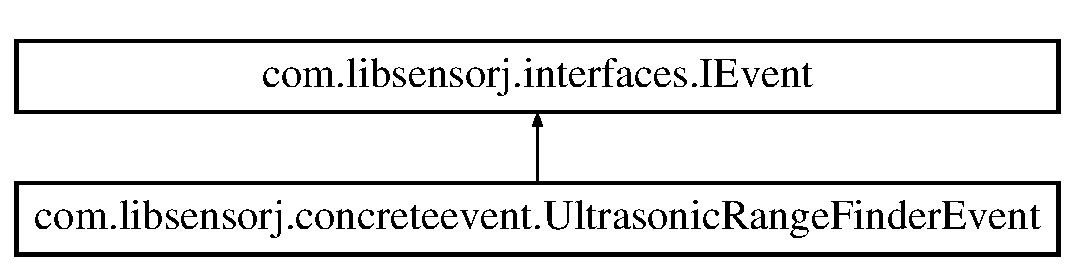
\includegraphics[height=2.000000cm]{classcom_1_1libsensorj_1_1concreteevent_1_1UltrasonicRangeFinderEvent}
\end{center}
\end{figure}
\subsection*{Public Member Functions}
\begin{DoxyCompactItemize}
\item 
void \hyperlink{classcom_1_1libsensorj_1_1concreteevent_1_1UltrasonicRangeFinderEvent_a0b32d3efeb55247269b4f43e4e34fe8e}{attach} (\hyperlink{classcom_1_1libsensorj_1_1model_1_1Observer}{Observer} obsever)
\item 
void \hyperlink{classcom_1_1libsensorj_1_1concreteevent_1_1UltrasonicRangeFinderEvent_ab0647f65e87ff07f61b3e4fe7e1daa19}{detach} (\hyperlink{classcom_1_1libsensorj_1_1model_1_1Observer}{Observer} obsever)
\item 
void \hyperlink{classcom_1_1libsensorj_1_1concreteevent_1_1UltrasonicRangeFinderEvent_a4d1ba316d1d324c4fb6e321e4c7a7b6e}{trigger} ()
\end{DoxyCompactItemize}


\subsection{Member Function Documentation}
\hypertarget{classcom_1_1libsensorj_1_1concreteevent_1_1UltrasonicRangeFinderEvent_a0b32d3efeb55247269b4f43e4e34fe8e}{}\index{com\+::libsensorj\+::concreteevent\+::\+Ultrasonic\+Range\+Finder\+Event@{com\+::libsensorj\+::concreteevent\+::\+Ultrasonic\+Range\+Finder\+Event}!attach@{attach}}
\index{attach@{attach}!com\+::libsensorj\+::concreteevent\+::\+Ultrasonic\+Range\+Finder\+Event@{com\+::libsensorj\+::concreteevent\+::\+Ultrasonic\+Range\+Finder\+Event}}
\subsubsection[{attach}]{\setlength{\rightskip}{0pt plus 5cm}void com.\+libsensorj.\+concreteevent.\+Ultrasonic\+Range\+Finder\+Event.\+attach (
\begin{DoxyParamCaption}
\item[{{\bf Observer}}]{obsever}
\end{DoxyParamCaption}
)}\label{classcom_1_1libsensorj_1_1concreteevent_1_1UltrasonicRangeFinderEvent_a0b32d3efeb55247269b4f43e4e34fe8e}


Implements \hyperlink{interfacecom_1_1libsensorj_1_1interfaces_1_1IEvent_af5af4301ccb6670452419d68baddf372}{com.\+libsensorj.\+interfaces.\+I\+Event}.

\hypertarget{classcom_1_1libsensorj_1_1concreteevent_1_1UltrasonicRangeFinderEvent_ab0647f65e87ff07f61b3e4fe7e1daa19}{}\index{com\+::libsensorj\+::concreteevent\+::\+Ultrasonic\+Range\+Finder\+Event@{com\+::libsensorj\+::concreteevent\+::\+Ultrasonic\+Range\+Finder\+Event}!detach@{detach}}
\index{detach@{detach}!com\+::libsensorj\+::concreteevent\+::\+Ultrasonic\+Range\+Finder\+Event@{com\+::libsensorj\+::concreteevent\+::\+Ultrasonic\+Range\+Finder\+Event}}
\subsubsection[{detach}]{\setlength{\rightskip}{0pt plus 5cm}void com.\+libsensorj.\+concreteevent.\+Ultrasonic\+Range\+Finder\+Event.\+detach (
\begin{DoxyParamCaption}
\item[{{\bf Observer}}]{obsever}
\end{DoxyParamCaption}
)}\label{classcom_1_1libsensorj_1_1concreteevent_1_1UltrasonicRangeFinderEvent_ab0647f65e87ff07f61b3e4fe7e1daa19}


Implements \hyperlink{interfacecom_1_1libsensorj_1_1interfaces_1_1IEvent_a974b07df97fda9f3be8e4afcd46470b2}{com.\+libsensorj.\+interfaces.\+I\+Event}.

\hypertarget{classcom_1_1libsensorj_1_1concreteevent_1_1UltrasonicRangeFinderEvent_a4d1ba316d1d324c4fb6e321e4c7a7b6e}{}\index{com\+::libsensorj\+::concreteevent\+::\+Ultrasonic\+Range\+Finder\+Event@{com\+::libsensorj\+::concreteevent\+::\+Ultrasonic\+Range\+Finder\+Event}!trigger@{trigger}}
\index{trigger@{trigger}!com\+::libsensorj\+::concreteevent\+::\+Ultrasonic\+Range\+Finder\+Event@{com\+::libsensorj\+::concreteevent\+::\+Ultrasonic\+Range\+Finder\+Event}}
\subsubsection[{trigger}]{\setlength{\rightskip}{0pt plus 5cm}void com.\+libsensorj.\+concreteevent.\+Ultrasonic\+Range\+Finder\+Event.\+trigger (
\begin{DoxyParamCaption}
{}
\end{DoxyParamCaption}
)}\label{classcom_1_1libsensorj_1_1concreteevent_1_1UltrasonicRangeFinderEvent_a4d1ba316d1d324c4fb6e321e4c7a7b6e}


Implements \hyperlink{interfacecom_1_1libsensorj_1_1interfaces_1_1IEvent_a861dea0956f77dd82f95e0110b8043b2}{com.\+libsensorj.\+interfaces.\+I\+Event}.



The documentation for this class was generated from the following file\+:\begin{DoxyCompactItemize}
\item 
main/java/com/libsensorj/concreteevent/\hyperlink{UltrasonicRangeFinderEvent_8java}{Ultrasonic\+Range\+Finder\+Event.\+java}\end{DoxyCompactItemize}

\hypertarget{classcom_1_1libsensorj_1_1examples_1_1UltrasonicRangeFinderExample}{}\section{com.\+libsensorj.\+examples.\+Ultrasonic\+Range\+Finder\+Example Class Reference}
\label{classcom_1_1libsensorj_1_1examples_1_1UltrasonicRangeFinderExample}\index{com.\+libsensorj.\+examples.\+Ultrasonic\+Range\+Finder\+Example@{com.\+libsensorj.\+examples.\+Ultrasonic\+Range\+Finder\+Example}}
\subsection*{Static Public Member Functions}
\begin{DoxyCompactItemize}
\item 
static void \hyperlink{classcom_1_1libsensorj_1_1examples_1_1UltrasonicRangeFinderExample_a587a298526337ce9e0d1fbbb9f400180}{main} (String\mbox{[}$\,$\mbox{]} args)
\end{DoxyCompactItemize}
\subsection*{Static Private Attributes}
\begin{DoxyCompactItemize}
\item 
static \hyperlink{interfacecom_1_1libsensorj_1_1interfaces_1_1ISensor}{I\+Sensor} \hyperlink{classcom_1_1libsensorj_1_1examples_1_1UltrasonicRangeFinderExample_af4703590c0c8bce89386204ea46afc76}{hcsr}
\item 
static final Logger \hyperlink{classcom_1_1libsensorj_1_1examples_1_1UltrasonicRangeFinderExample_ac1d433a89455addc211f404fe522f0ec}{L\+O\+G\+G\+E\+R}
\end{DoxyCompactItemize}


\subsection{Detailed Description}
The Class \hyperlink{classcom_1_1libsensorj_1_1examples_1_1UltrasonicRangeFinderExample}{Ultrasonic\+Range\+Finder\+Example}. 

\subsection{Member Function Documentation}
\hypertarget{classcom_1_1libsensorj_1_1examples_1_1UltrasonicRangeFinderExample_a587a298526337ce9e0d1fbbb9f400180}{}\index{com\+::libsensorj\+::examples\+::\+Ultrasonic\+Range\+Finder\+Example@{com\+::libsensorj\+::examples\+::\+Ultrasonic\+Range\+Finder\+Example}!main@{main}}
\index{main@{main}!com\+::libsensorj\+::examples\+::\+Ultrasonic\+Range\+Finder\+Example@{com\+::libsensorj\+::examples\+::\+Ultrasonic\+Range\+Finder\+Example}}
\subsubsection[{main}]{\setlength{\rightskip}{0pt plus 5cm}static void com.\+libsensorj.\+examples.\+Ultrasonic\+Range\+Finder\+Example.\+main (
\begin{DoxyParamCaption}
\item[{String\mbox{[}$\,$\mbox{]}}]{args}
\end{DoxyParamCaption}
)\hspace{0.3cm}{\ttfamily [static]}}\label{classcom_1_1libsensorj_1_1examples_1_1UltrasonicRangeFinderExample_a587a298526337ce9e0d1fbbb9f400180}
The main method.


\begin{DoxyParams}{Parameters}
{\em args} & the arguments \\
\hline
\end{DoxyParams}


\subsection{Member Data Documentation}
\hypertarget{classcom_1_1libsensorj_1_1examples_1_1UltrasonicRangeFinderExample_af4703590c0c8bce89386204ea46afc76}{}\index{com\+::libsensorj\+::examples\+::\+Ultrasonic\+Range\+Finder\+Example@{com\+::libsensorj\+::examples\+::\+Ultrasonic\+Range\+Finder\+Example}!hcsr@{hcsr}}
\index{hcsr@{hcsr}!com\+::libsensorj\+::examples\+::\+Ultrasonic\+Range\+Finder\+Example@{com\+::libsensorj\+::examples\+::\+Ultrasonic\+Range\+Finder\+Example}}
\subsubsection[{hcsr}]{\setlength{\rightskip}{0pt plus 5cm}{\bf I\+Sensor} com.\+libsensorj.\+examples.\+Ultrasonic\+Range\+Finder\+Example.\+hcsr\hspace{0.3cm}{\ttfamily [static]}, {\ttfamily [private]}}\label{classcom_1_1libsensorj_1_1examples_1_1UltrasonicRangeFinderExample_af4703590c0c8bce89386204ea46afc76}
The I\+Sensor hcsr. \hypertarget{classcom_1_1libsensorj_1_1examples_1_1UltrasonicRangeFinderExample_ac1d433a89455addc211f404fe522f0ec}{}\index{com\+::libsensorj\+::examples\+::\+Ultrasonic\+Range\+Finder\+Example@{com\+::libsensorj\+::examples\+::\+Ultrasonic\+Range\+Finder\+Example}!L\+O\+G\+G\+E\+R@{L\+O\+G\+G\+E\+R}}
\index{L\+O\+G\+G\+E\+R@{L\+O\+G\+G\+E\+R}!com\+::libsensorj\+::examples\+::\+Ultrasonic\+Range\+Finder\+Example@{com\+::libsensorj\+::examples\+::\+Ultrasonic\+Range\+Finder\+Example}}
\subsubsection[{L\+O\+G\+G\+E\+R}]{\setlength{\rightskip}{0pt plus 5cm}final Logger com.\+libsensorj.\+examples.\+Ultrasonic\+Range\+Finder\+Example.\+L\+O\+G\+G\+E\+R\hspace{0.3cm}{\ttfamily [static]}, {\ttfamily [private]}}\label{classcom_1_1libsensorj_1_1examples_1_1UltrasonicRangeFinderExample_ac1d433a89455addc211f404fe522f0ec}
{\bfseries Initial value\+:}
\begin{DoxyCode}
= LogManager
            .getLogger(UltrasonicRangeFinderExample.class.getName())
\end{DoxyCode}
The Constant L\+O\+G\+G\+E\+R. 

The documentation for this class was generated from the following file\+:\begin{DoxyCompactItemize}
\item 
main/java/com/libsensorj/examples/\hyperlink{UltrasonicRangeFinderExample_8java}{Ultrasonic\+Range\+Finder\+Example.\+java}\end{DoxyCompactItemize}

\hypertarget{classcom_1_1libsensorj_1_1concretefactory_1_1UltrasonicRangeFinderFactory}{}\section{com.\+libsensorj.\+concretefactory.\+Ultrasonic\+Range\+Finder\+Factory Class Reference}
\label{classcom_1_1libsensorj_1_1concretefactory_1_1UltrasonicRangeFinderFactory}\index{com.\+libsensorj.\+concretefactory.\+Ultrasonic\+Range\+Finder\+Factory@{com.\+libsensorj.\+concretefactory.\+Ultrasonic\+Range\+Finder\+Factory}}
Inheritance diagram for com.\+libsensorj.\+concretefactory.\+Ultrasonic\+Range\+Finder\+Factory\+:\begin{figure}[H]
\begin{center}
\leavevmode
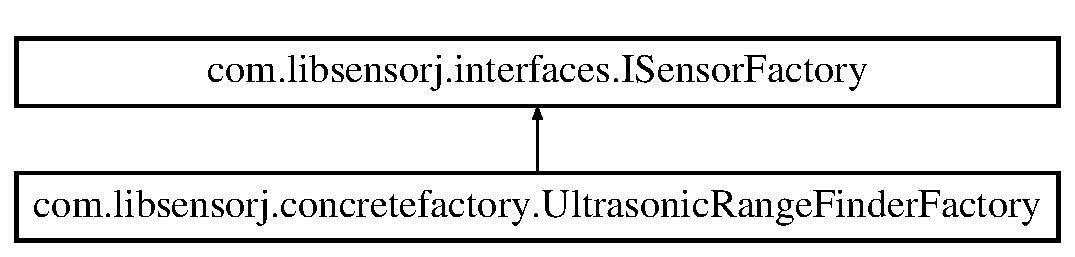
\includegraphics[height=2.000000cm]{classcom_1_1libsensorj_1_1concretefactory_1_1UltrasonicRangeFinderFactory}
\end{center}
\end{figure}
\subsection*{Public Member Functions}
\begin{DoxyCompactItemize}
\item 
\hyperlink{interfacecom_1_1libsensorj_1_1interfaces_1_1ISensor}{I\+Sensor} \hyperlink{classcom_1_1libsensorj_1_1concretefactory_1_1UltrasonicRangeFinderFactory_a3aa6e46ef47bf97355df4d5cfb1b1e01}{create\+Sensor} ()
\item 
\hyperlink{interfacecom_1_1libsensorj_1_1interfaces_1_1IEvent}{I\+Event} \hyperlink{classcom_1_1libsensorj_1_1concretefactory_1_1UltrasonicRangeFinderFactory_a8a7d0c55346f1ab5630a878f6a3175fd}{create\+Event} ()
\end{DoxyCompactItemize}


\subsection{Member Function Documentation}
\hypertarget{classcom_1_1libsensorj_1_1concretefactory_1_1UltrasonicRangeFinderFactory_a8a7d0c55346f1ab5630a878f6a3175fd}{}\index{com\+::libsensorj\+::concretefactory\+::\+Ultrasonic\+Range\+Finder\+Factory@{com\+::libsensorj\+::concretefactory\+::\+Ultrasonic\+Range\+Finder\+Factory}!create\+Event@{create\+Event}}
\index{create\+Event@{create\+Event}!com\+::libsensorj\+::concretefactory\+::\+Ultrasonic\+Range\+Finder\+Factory@{com\+::libsensorj\+::concretefactory\+::\+Ultrasonic\+Range\+Finder\+Factory}}
\subsubsection[{create\+Event}]{\setlength{\rightskip}{0pt plus 5cm}{\bf I\+Event} com.\+libsensorj.\+concretefactory.\+Ultrasonic\+Range\+Finder\+Factory.\+create\+Event (
\begin{DoxyParamCaption}
{}
\end{DoxyParamCaption}
)}\label{classcom_1_1libsensorj_1_1concretefactory_1_1UltrasonicRangeFinderFactory_a8a7d0c55346f1ab5630a878f6a3175fd}


Implements \hyperlink{interfacecom_1_1libsensorj_1_1interfaces_1_1ISensorFactory_a2b074d01287a4e64677097255ba9e768}{com.\+libsensorj.\+interfaces.\+I\+Sensor\+Factory}.

\hypertarget{classcom_1_1libsensorj_1_1concretefactory_1_1UltrasonicRangeFinderFactory_a3aa6e46ef47bf97355df4d5cfb1b1e01}{}\index{com\+::libsensorj\+::concretefactory\+::\+Ultrasonic\+Range\+Finder\+Factory@{com\+::libsensorj\+::concretefactory\+::\+Ultrasonic\+Range\+Finder\+Factory}!create\+Sensor@{create\+Sensor}}
\index{create\+Sensor@{create\+Sensor}!com\+::libsensorj\+::concretefactory\+::\+Ultrasonic\+Range\+Finder\+Factory@{com\+::libsensorj\+::concretefactory\+::\+Ultrasonic\+Range\+Finder\+Factory}}
\subsubsection[{create\+Sensor}]{\setlength{\rightskip}{0pt plus 5cm}{\bf I\+Sensor} com.\+libsensorj.\+concretefactory.\+Ultrasonic\+Range\+Finder\+Factory.\+create\+Sensor (
\begin{DoxyParamCaption}
{}
\end{DoxyParamCaption}
)}\label{classcom_1_1libsensorj_1_1concretefactory_1_1UltrasonicRangeFinderFactory_a3aa6e46ef47bf97355df4d5cfb1b1e01}


Implements \hyperlink{interfacecom_1_1libsensorj_1_1interfaces_1_1ISensorFactory_ac14c6d566c37c6a79c6db1e85634f25d}{com.\+libsensorj.\+interfaces.\+I\+Sensor\+Factory}.



The documentation for this class was generated from the following file\+:\begin{DoxyCompactItemize}
\item 
main/java/com/libsensorj/concretefactory/\hyperlink{UltrasonicRangeFinderFactory_8java}{Ultrasonic\+Range\+Finder\+Factory.\+java}\end{DoxyCompactItemize}

\hypertarget{classcom_1_1pi4j_1_1examples_1_1UsageGpioExample}{}\section{com.\+pi4j.\+examples.\+Usage\+Gpio\+Example Class Reference}
\label{classcom_1_1pi4j_1_1examples_1_1UsageGpioExample}\index{com.\+pi4j.\+examples.\+Usage\+Gpio\+Example@{com.\+pi4j.\+examples.\+Usage\+Gpio\+Example}}
\subsection*{Classes}
\begin{DoxyCompactItemize}
\item 
class \hyperlink{classcom_1_1pi4j_1_1examples_1_1UsageGpioExample_1_1GpioUsageExampleListener}{Gpio\+Usage\+Example\+Listener}
\end{DoxyCompactItemize}
\subsection*{Static Public Member Functions}
\begin{DoxyCompactItemize}
\item 
static void \hyperlink{classcom_1_1pi4j_1_1examples_1_1UsageGpioExample_a3e0037b97996d49eafd6b96102d6e248}{main} (String\mbox{[}$\,$\mbox{]} args)  throws Interrupted\+Exception 
\end{DoxyCompactItemize}
\subsection*{Static Private Attributes}
\begin{DoxyCompactItemize}
\item 
static final Logger \hyperlink{classcom_1_1pi4j_1_1examples_1_1UsageGpioExample_a1cff0316c22ecf42864e50c3487256b9}{L\+O\+G\+G\+E\+R}
\end{DoxyCompactItemize}


\subsection{Detailed Description}
This example code demonstrates how to setup simple triggers for G\+P\+I\+O pins on the Raspberry Pi.

\begin{DoxyAuthor}{Author}
Robert Savage 
\end{DoxyAuthor}


\subsection{Member Function Documentation}
\hypertarget{classcom_1_1pi4j_1_1examples_1_1UsageGpioExample_a3e0037b97996d49eafd6b96102d6e248}{}\index{com\+::pi4j\+::examples\+::\+Usage\+Gpio\+Example@{com\+::pi4j\+::examples\+::\+Usage\+Gpio\+Example}!main@{main}}
\index{main@{main}!com\+::pi4j\+::examples\+::\+Usage\+Gpio\+Example@{com\+::pi4j\+::examples\+::\+Usage\+Gpio\+Example}}
\subsubsection[{main}]{\setlength{\rightskip}{0pt plus 5cm}static void com.\+pi4j.\+examples.\+Usage\+Gpio\+Example.\+main (
\begin{DoxyParamCaption}
\item[{String\mbox{[}$\,$\mbox{]}}]{args}
\end{DoxyParamCaption}
) throws Interrupted\+Exception\hspace{0.3cm}{\ttfamily [static]}}\label{classcom_1_1pi4j_1_1examples_1_1UsageGpioExample_a3e0037b97996d49eafd6b96102d6e248}


\subsection{Member Data Documentation}
\hypertarget{classcom_1_1pi4j_1_1examples_1_1UsageGpioExample_a1cff0316c22ecf42864e50c3487256b9}{}\index{com\+::pi4j\+::examples\+::\+Usage\+Gpio\+Example@{com\+::pi4j\+::examples\+::\+Usage\+Gpio\+Example}!L\+O\+G\+G\+E\+R@{L\+O\+G\+G\+E\+R}}
\index{L\+O\+G\+G\+E\+R@{L\+O\+G\+G\+E\+R}!com\+::pi4j\+::examples\+::\+Usage\+Gpio\+Example@{com\+::pi4j\+::examples\+::\+Usage\+Gpio\+Example}}
\subsubsection[{L\+O\+G\+G\+E\+R}]{\setlength{\rightskip}{0pt plus 5cm}final Logger com.\+pi4j.\+examples.\+Usage\+Gpio\+Example.\+L\+O\+G\+G\+E\+R\hspace{0.3cm}{\ttfamily [static]}, {\ttfamily [private]}}\label{classcom_1_1pi4j_1_1examples_1_1UsageGpioExample_a1cff0316c22ecf42864e50c3487256b9}
{\bfseries Initial value\+:}
\begin{DoxyCode}
= LogManager
            .getLogger(UsageGpioExample.class.getName())
\end{DoxyCode}


The documentation for this class was generated from the following file\+:\begin{DoxyCompactItemize}
\item 
main/java/com/pi4j/examples/\hyperlink{UsageGpioExample_8java}{Usage\+Gpio\+Example.\+java}\end{DoxyCompactItemize}

\hypertarget{classcom_1_1pi4j_1_1examples_1_1I2CWiiMotionPlusExample_1_1WiiMotionPlus}{}\section{com.\+pi4j.\+examples.\+I2\+C\+Wii\+Motion\+Plus\+Example.\+Wii\+Motion\+Plus Class Reference}
\label{classcom_1_1pi4j_1_1examples_1_1I2CWiiMotionPlusExample_1_1WiiMotionPlus}\index{com.\+pi4j.\+examples.\+I2\+C\+Wii\+Motion\+Plus\+Example.\+Wii\+Motion\+Plus@{com.\+pi4j.\+examples.\+I2\+C\+Wii\+Motion\+Plus\+Example.\+Wii\+Motion\+Plus}}
\subsection*{Public Member Functions}
\begin{DoxyCompactItemize}
\item 
\hyperlink{classcom_1_1pi4j_1_1examples_1_1I2CWiiMotionPlusExample_1_1WiiMotionPlus_abc6322249b2383c60a87edc5d38dc38f}{Wii\+Motion\+Plus} (I2\+C\+Bus bus)  throws I\+O\+Exception 
\item 
void \hyperlink{classcom_1_1pi4j_1_1examples_1_1I2CWiiMotionPlusExample_1_1WiiMotionPlus_a1344433cd4b813caab9433b254a1c9e3}{init} ()
\item 
\hyperlink{classcom_1_1pi4j_1_1examples_1_1I2CWiiMotionPlusExample_1_1ThreeAxis}{Three\+Axis} \hyperlink{classcom_1_1pi4j_1_1examples_1_1I2CWiiMotionPlusExample_1_1WiiMotionPlus_ac46ff1a05559eb5780ca1e28255d8cea}{read} ()  throws I\+O\+Exception 
\end{DoxyCompactItemize}
\subsection*{Private Member Functions}
\begin{DoxyCompactItemize}
\item 
int \hyperlink{classcom_1_1pi4j_1_1examples_1_1I2CWiiMotionPlusExample_1_1WiiMotionPlus_a5706e1080e6935ba9ed9516db278ee4b}{as\+Int} (byte b)
\end{DoxyCompactItemize}
\subsection*{Private Attributes}
\begin{DoxyCompactItemize}
\item 
I2\+C\+Device \hyperlink{classcom_1_1pi4j_1_1examples_1_1I2CWiiMotionPlusExample_1_1WiiMotionPlus_a8caa866617964bc9c0f60980d8f5ddec}{init\+Device}
\item 
I2\+C\+Device \hyperlink{classcom_1_1pi4j_1_1examples_1_1I2CWiiMotionPlusExample_1_1WiiMotionPlus_a5785ab1b5e1108c36e1286c489a3684b}{device}
\end{DoxyCompactItemize}


\subsection{Constructor \& Destructor Documentation}
\hypertarget{classcom_1_1pi4j_1_1examples_1_1I2CWiiMotionPlusExample_1_1WiiMotionPlus_abc6322249b2383c60a87edc5d38dc38f}{}\index{com\+::pi4j\+::examples\+::\+I2\+C\+Wii\+Motion\+Plus\+Example\+::\+Wii\+Motion\+Plus@{com\+::pi4j\+::examples\+::\+I2\+C\+Wii\+Motion\+Plus\+Example\+::\+Wii\+Motion\+Plus}!Wii\+Motion\+Plus@{Wii\+Motion\+Plus}}
\index{Wii\+Motion\+Plus@{Wii\+Motion\+Plus}!com\+::pi4j\+::examples\+::\+I2\+C\+Wii\+Motion\+Plus\+Example\+::\+Wii\+Motion\+Plus@{com\+::pi4j\+::examples\+::\+I2\+C\+Wii\+Motion\+Plus\+Example\+::\+Wii\+Motion\+Plus}}
\subsubsection[{Wii\+Motion\+Plus}]{\setlength{\rightskip}{0pt plus 5cm}com.\+pi4j.\+examples.\+I2\+C\+Wii\+Motion\+Plus\+Example.\+Wii\+Motion\+Plus.\+Wii\+Motion\+Plus (
\begin{DoxyParamCaption}
\item[{I2\+C\+Bus}]{bus}
\end{DoxyParamCaption}
) throws I\+O\+Exception}\label{classcom_1_1pi4j_1_1examples_1_1I2CWiiMotionPlusExample_1_1WiiMotionPlus_abc6322249b2383c60a87edc5d38dc38f}


\subsection{Member Function Documentation}
\hypertarget{classcom_1_1pi4j_1_1examples_1_1I2CWiiMotionPlusExample_1_1WiiMotionPlus_a5706e1080e6935ba9ed9516db278ee4b}{}\index{com\+::pi4j\+::examples\+::\+I2\+C\+Wii\+Motion\+Plus\+Example\+::\+Wii\+Motion\+Plus@{com\+::pi4j\+::examples\+::\+I2\+C\+Wii\+Motion\+Plus\+Example\+::\+Wii\+Motion\+Plus}!as\+Int@{as\+Int}}
\index{as\+Int@{as\+Int}!com\+::pi4j\+::examples\+::\+I2\+C\+Wii\+Motion\+Plus\+Example\+::\+Wii\+Motion\+Plus@{com\+::pi4j\+::examples\+::\+I2\+C\+Wii\+Motion\+Plus\+Example\+::\+Wii\+Motion\+Plus}}
\subsubsection[{as\+Int}]{\setlength{\rightskip}{0pt plus 5cm}int com.\+pi4j.\+examples.\+I2\+C\+Wii\+Motion\+Plus\+Example.\+Wii\+Motion\+Plus.\+as\+Int (
\begin{DoxyParamCaption}
\item[{byte}]{b}
\end{DoxyParamCaption}
)\hspace{0.3cm}{\ttfamily [private]}}\label{classcom_1_1pi4j_1_1examples_1_1I2CWiiMotionPlusExample_1_1WiiMotionPlus_a5706e1080e6935ba9ed9516db278ee4b}
\hypertarget{classcom_1_1pi4j_1_1examples_1_1I2CWiiMotionPlusExample_1_1WiiMotionPlus_a1344433cd4b813caab9433b254a1c9e3}{}\index{com\+::pi4j\+::examples\+::\+I2\+C\+Wii\+Motion\+Plus\+Example\+::\+Wii\+Motion\+Plus@{com\+::pi4j\+::examples\+::\+I2\+C\+Wii\+Motion\+Plus\+Example\+::\+Wii\+Motion\+Plus}!init@{init}}
\index{init@{init}!com\+::pi4j\+::examples\+::\+I2\+C\+Wii\+Motion\+Plus\+Example\+::\+Wii\+Motion\+Plus@{com\+::pi4j\+::examples\+::\+I2\+C\+Wii\+Motion\+Plus\+Example\+::\+Wii\+Motion\+Plus}}
\subsubsection[{init}]{\setlength{\rightskip}{0pt plus 5cm}void com.\+pi4j.\+examples.\+I2\+C\+Wii\+Motion\+Plus\+Example.\+Wii\+Motion\+Plus.\+init (
\begin{DoxyParamCaption}
{}
\end{DoxyParamCaption}
)}\label{classcom_1_1pi4j_1_1examples_1_1I2CWiiMotionPlusExample_1_1WiiMotionPlus_a1344433cd4b813caab9433b254a1c9e3}
\hypertarget{classcom_1_1pi4j_1_1examples_1_1I2CWiiMotionPlusExample_1_1WiiMotionPlus_ac46ff1a05559eb5780ca1e28255d8cea}{}\index{com\+::pi4j\+::examples\+::\+I2\+C\+Wii\+Motion\+Plus\+Example\+::\+Wii\+Motion\+Plus@{com\+::pi4j\+::examples\+::\+I2\+C\+Wii\+Motion\+Plus\+Example\+::\+Wii\+Motion\+Plus}!read@{read}}
\index{read@{read}!com\+::pi4j\+::examples\+::\+I2\+C\+Wii\+Motion\+Plus\+Example\+::\+Wii\+Motion\+Plus@{com\+::pi4j\+::examples\+::\+I2\+C\+Wii\+Motion\+Plus\+Example\+::\+Wii\+Motion\+Plus}}
\subsubsection[{read}]{\setlength{\rightskip}{0pt plus 5cm}{\bf Three\+Axis} com.\+pi4j.\+examples.\+I2\+C\+Wii\+Motion\+Plus\+Example.\+Wii\+Motion\+Plus.\+read (
\begin{DoxyParamCaption}
{}
\end{DoxyParamCaption}
) throws I\+O\+Exception}\label{classcom_1_1pi4j_1_1examples_1_1I2CWiiMotionPlusExample_1_1WiiMotionPlus_ac46ff1a05559eb5780ca1e28255d8cea}


\subsection{Member Data Documentation}
\hypertarget{classcom_1_1pi4j_1_1examples_1_1I2CWiiMotionPlusExample_1_1WiiMotionPlus_a5785ab1b5e1108c36e1286c489a3684b}{}\index{com\+::pi4j\+::examples\+::\+I2\+C\+Wii\+Motion\+Plus\+Example\+::\+Wii\+Motion\+Plus@{com\+::pi4j\+::examples\+::\+I2\+C\+Wii\+Motion\+Plus\+Example\+::\+Wii\+Motion\+Plus}!device@{device}}
\index{device@{device}!com\+::pi4j\+::examples\+::\+I2\+C\+Wii\+Motion\+Plus\+Example\+::\+Wii\+Motion\+Plus@{com\+::pi4j\+::examples\+::\+I2\+C\+Wii\+Motion\+Plus\+Example\+::\+Wii\+Motion\+Plus}}
\subsubsection[{device}]{\setlength{\rightskip}{0pt plus 5cm}I2\+C\+Device com.\+pi4j.\+examples.\+I2\+C\+Wii\+Motion\+Plus\+Example.\+Wii\+Motion\+Plus.\+device\hspace{0.3cm}{\ttfamily [private]}}\label{classcom_1_1pi4j_1_1examples_1_1I2CWiiMotionPlusExample_1_1WiiMotionPlus_a5785ab1b5e1108c36e1286c489a3684b}
\hypertarget{classcom_1_1pi4j_1_1examples_1_1I2CWiiMotionPlusExample_1_1WiiMotionPlus_a8caa866617964bc9c0f60980d8f5ddec}{}\index{com\+::pi4j\+::examples\+::\+I2\+C\+Wii\+Motion\+Plus\+Example\+::\+Wii\+Motion\+Plus@{com\+::pi4j\+::examples\+::\+I2\+C\+Wii\+Motion\+Plus\+Example\+::\+Wii\+Motion\+Plus}!init\+Device@{init\+Device}}
\index{init\+Device@{init\+Device}!com\+::pi4j\+::examples\+::\+I2\+C\+Wii\+Motion\+Plus\+Example\+::\+Wii\+Motion\+Plus@{com\+::pi4j\+::examples\+::\+I2\+C\+Wii\+Motion\+Plus\+Example\+::\+Wii\+Motion\+Plus}}
\subsubsection[{init\+Device}]{\setlength{\rightskip}{0pt plus 5cm}I2\+C\+Device com.\+pi4j.\+examples.\+I2\+C\+Wii\+Motion\+Plus\+Example.\+Wii\+Motion\+Plus.\+init\+Device\hspace{0.3cm}{\ttfamily [private]}}\label{classcom_1_1pi4j_1_1examples_1_1I2CWiiMotionPlusExample_1_1WiiMotionPlus_a8caa866617964bc9c0f60980d8f5ddec}


The documentation for this class was generated from the following file\+:\begin{DoxyCompactItemize}
\item 
main/java/com/pi4j/examples/\hyperlink{I2CWiiMotionPlusExample_8java}{I2\+C\+Wii\+Motion\+Plus\+Example.\+java}\end{DoxyCompactItemize}

\hypertarget{classcom_1_1pi4j_1_1examples_1_1WiringPiGpioExample}{}\section{com.\+pi4j.\+examples.\+Wiring\+Pi\+Gpio\+Example Class Reference}
\label{classcom_1_1pi4j_1_1examples_1_1WiringPiGpioExample}\index{com.\+pi4j.\+examples.\+Wiring\+Pi\+Gpio\+Example@{com.\+pi4j.\+examples.\+Wiring\+Pi\+Gpio\+Example}}
\subsection*{Static Public Member Functions}
\begin{DoxyCompactItemize}
\item 
static void \hyperlink{classcom_1_1pi4j_1_1examples_1_1WiringPiGpioExample_a08ba708384c8be2fe95de5abd7355a8e}{main} (String\mbox{[}$\,$\mbox{]} args)  throws Interrupted\+Exception 
\end{DoxyCompactItemize}
\subsection*{Static Private Attributes}
\begin{DoxyCompactItemize}
\item 
static final Logger \hyperlink{classcom_1_1pi4j_1_1examples_1_1WiringPiGpioExample_a921e49acca89ed226d4f6be6e1eba1b6}{L\+O\+G\+G\+E\+R}
\item 
static final int\mbox{[}$\,$\mbox{]} \hyperlink{classcom_1_1pi4j_1_1examples_1_1WiringPiGpioExample_a572ac65411fd1bff9c8ff4520800471a}{D\+A\+T\+A}
\end{DoxyCompactItemize}


\subsection{Member Function Documentation}
\hypertarget{classcom_1_1pi4j_1_1examples_1_1WiringPiGpioExample_a08ba708384c8be2fe95de5abd7355a8e}{}\index{com\+::pi4j\+::examples\+::\+Wiring\+Pi\+Gpio\+Example@{com\+::pi4j\+::examples\+::\+Wiring\+Pi\+Gpio\+Example}!main@{main}}
\index{main@{main}!com\+::pi4j\+::examples\+::\+Wiring\+Pi\+Gpio\+Example@{com\+::pi4j\+::examples\+::\+Wiring\+Pi\+Gpio\+Example}}
\subsubsection[{main}]{\setlength{\rightskip}{0pt plus 5cm}static void com.\+pi4j.\+examples.\+Wiring\+Pi\+Gpio\+Example.\+main (
\begin{DoxyParamCaption}
\item[{String\mbox{[}$\,$\mbox{]}}]{args}
\end{DoxyParamCaption}
) throws Interrupted\+Exception\hspace{0.3cm}{\ttfamily [static]}}\label{classcom_1_1pi4j_1_1examples_1_1WiringPiGpioExample_a08ba708384c8be2fe95de5abd7355a8e}


\subsection{Member Data Documentation}
\hypertarget{classcom_1_1pi4j_1_1examples_1_1WiringPiGpioExample_a572ac65411fd1bff9c8ff4520800471a}{}\index{com\+::pi4j\+::examples\+::\+Wiring\+Pi\+Gpio\+Example@{com\+::pi4j\+::examples\+::\+Wiring\+Pi\+Gpio\+Example}!D\+A\+T\+A@{D\+A\+T\+A}}
\index{D\+A\+T\+A@{D\+A\+T\+A}!com\+::pi4j\+::examples\+::\+Wiring\+Pi\+Gpio\+Example@{com\+::pi4j\+::examples\+::\+Wiring\+Pi\+Gpio\+Example}}
\subsubsection[{D\+A\+T\+A}]{\setlength{\rightskip}{0pt plus 5cm}final int \mbox{[}$\,$\mbox{]} com.\+pi4j.\+examples.\+Wiring\+Pi\+Gpio\+Example.\+D\+A\+T\+A\hspace{0.3cm}{\ttfamily [static]}, {\ttfamily [private]}}\label{classcom_1_1pi4j_1_1examples_1_1WiringPiGpioExample_a572ac65411fd1bff9c8ff4520800471a}
{\bfseries Initial value\+:}
\begin{DoxyCode}
= \{ 0, 1, 1, 1, 1, 1, 0, 0, 0, 2, 1, 1, 1,
            0, 0, 3, 1, 1, 2, 0, 0, 4, 1, 1, 3, 0, 0, 5, 1, 1, 4, 0, 0, 6, 1,
            1, 5, 0, 0, 7, 1, 1, 6, 0, 1, 7, 0, 1,
            0,
            0,
            
            1,
            
            7, 1, 1, 6, 1, 1, 7, 0, 0, 5, 1, 1, 6, 0, 0, 4, 1, 1, 5, 0, 0, 3,
            1, 1, 4, 0, 0, 2, 1, 1, 3, 0, 0, 1, 1, 1, 2, 0, 0, 0, 1, 1, 1, 0,
            1, 0, 0, 1, 0, 0,
            
            1, 9, 9, 9,
    
    \}
\end{DoxyCode}
\hypertarget{classcom_1_1pi4j_1_1examples_1_1WiringPiGpioExample_a921e49acca89ed226d4f6be6e1eba1b6}{}\index{com\+::pi4j\+::examples\+::\+Wiring\+Pi\+Gpio\+Example@{com\+::pi4j\+::examples\+::\+Wiring\+Pi\+Gpio\+Example}!L\+O\+G\+G\+E\+R@{L\+O\+G\+G\+E\+R}}
\index{L\+O\+G\+G\+E\+R@{L\+O\+G\+G\+E\+R}!com\+::pi4j\+::examples\+::\+Wiring\+Pi\+Gpio\+Example@{com\+::pi4j\+::examples\+::\+Wiring\+Pi\+Gpio\+Example}}
\subsubsection[{L\+O\+G\+G\+E\+R}]{\setlength{\rightskip}{0pt plus 5cm}final Logger com.\+pi4j.\+examples.\+Wiring\+Pi\+Gpio\+Example.\+L\+O\+G\+G\+E\+R\hspace{0.3cm}{\ttfamily [static]}, {\ttfamily [private]}}\label{classcom_1_1pi4j_1_1examples_1_1WiringPiGpioExample_a921e49acca89ed226d4f6be6e1eba1b6}
{\bfseries Initial value\+:}
\begin{DoxyCode}
= LogManager
            .getLogger(WiringPiGpioExample.class.getName())
\end{DoxyCode}


The documentation for this class was generated from the following file\+:\begin{DoxyCompactItemize}
\item 
main/java/com/pi4j/examples/\hyperlink{WiringPiGpioExample_8java}{Wiring\+Pi\+Gpio\+Example.\+java}\end{DoxyCompactItemize}

\hypertarget{classcom_1_1pi4j_1_1examples_1_1WiringPiGpioInterruptExample}{}\section{com.\+pi4j.\+examples.\+Wiring\+Pi\+Gpio\+Interrupt\+Example Class Reference}
\label{classcom_1_1pi4j_1_1examples_1_1WiringPiGpioInterruptExample}\index{com.\+pi4j.\+examples.\+Wiring\+Pi\+Gpio\+Interrupt\+Example@{com.\+pi4j.\+examples.\+Wiring\+Pi\+Gpio\+Interrupt\+Example}}
\subsection*{Static Public Member Functions}
\begin{DoxyCompactItemize}
\item 
static void \hyperlink{classcom_1_1pi4j_1_1examples_1_1WiringPiGpioInterruptExample_a5061924ce17276bf4308661687013bda}{main} (String\mbox{[}$\,$\mbox{]} args)  throws Interrupted\+Exception 
\end{DoxyCompactItemize}
\subsection*{Static Private Attributes}
\begin{DoxyCompactItemize}
\item 
static final Logger \hyperlink{classcom_1_1pi4j_1_1examples_1_1WiringPiGpioInterruptExample_a2d2a1b14941113d371ddc16140d2dec1}{L\+O\+G\+G\+E\+R}
\end{DoxyCompactItemize}


\subsection{Member Function Documentation}
\hypertarget{classcom_1_1pi4j_1_1examples_1_1WiringPiGpioInterruptExample_a5061924ce17276bf4308661687013bda}{}\index{com\+::pi4j\+::examples\+::\+Wiring\+Pi\+Gpio\+Interrupt\+Example@{com\+::pi4j\+::examples\+::\+Wiring\+Pi\+Gpio\+Interrupt\+Example}!main@{main}}
\index{main@{main}!com\+::pi4j\+::examples\+::\+Wiring\+Pi\+Gpio\+Interrupt\+Example@{com\+::pi4j\+::examples\+::\+Wiring\+Pi\+Gpio\+Interrupt\+Example}}
\subsubsection[{main}]{\setlength{\rightskip}{0pt plus 5cm}static void com.\+pi4j.\+examples.\+Wiring\+Pi\+Gpio\+Interrupt\+Example.\+main (
\begin{DoxyParamCaption}
\item[{String\mbox{[}$\,$\mbox{]}}]{args}
\end{DoxyParamCaption}
) throws Interrupted\+Exception\hspace{0.3cm}{\ttfamily [static]}}\label{classcom_1_1pi4j_1_1examples_1_1WiringPiGpioInterruptExample_a5061924ce17276bf4308661687013bda}


\subsection{Member Data Documentation}
\hypertarget{classcom_1_1pi4j_1_1examples_1_1WiringPiGpioInterruptExample_a2d2a1b14941113d371ddc16140d2dec1}{}\index{com\+::pi4j\+::examples\+::\+Wiring\+Pi\+Gpio\+Interrupt\+Example@{com\+::pi4j\+::examples\+::\+Wiring\+Pi\+Gpio\+Interrupt\+Example}!L\+O\+G\+G\+E\+R@{L\+O\+G\+G\+E\+R}}
\index{L\+O\+G\+G\+E\+R@{L\+O\+G\+G\+E\+R}!com\+::pi4j\+::examples\+::\+Wiring\+Pi\+Gpio\+Interrupt\+Example@{com\+::pi4j\+::examples\+::\+Wiring\+Pi\+Gpio\+Interrupt\+Example}}
\subsubsection[{L\+O\+G\+G\+E\+R}]{\setlength{\rightskip}{0pt plus 5cm}final Logger com.\+pi4j.\+examples.\+Wiring\+Pi\+Gpio\+Interrupt\+Example.\+L\+O\+G\+G\+E\+R\hspace{0.3cm}{\ttfamily [static]}, {\ttfamily [private]}}\label{classcom_1_1pi4j_1_1examples_1_1WiringPiGpioInterruptExample_a2d2a1b14941113d371ddc16140d2dec1}
{\bfseries Initial value\+:}
\begin{DoxyCode}
= LogManager
            .getLogger(WiringPiGpioInterruptExample.class.getName())
\end{DoxyCode}


The documentation for this class was generated from the following file\+:\begin{DoxyCompactItemize}
\item 
main/java/com/pi4j/examples/\hyperlink{WiringPiGpioInterruptExample_8java}{Wiring\+Pi\+Gpio\+Interrupt\+Example.\+java}\end{DoxyCompactItemize}

\hypertarget{classcom_1_1pi4j_1_1examples_1_1WiringPiGpioInterruptExample2}{}\section{com.\+pi4j.\+examples.\+Wiring\+Pi\+Gpio\+Interrupt\+Example2 Class Reference}
\label{classcom_1_1pi4j_1_1examples_1_1WiringPiGpioInterruptExample2}\index{com.\+pi4j.\+examples.\+Wiring\+Pi\+Gpio\+Interrupt\+Example2@{com.\+pi4j.\+examples.\+Wiring\+Pi\+Gpio\+Interrupt\+Example2}}
\subsection*{Static Public Member Functions}
\begin{DoxyCompactItemize}
\item 
static void \hyperlink{classcom_1_1pi4j_1_1examples_1_1WiringPiGpioInterruptExample2_a52c618edef3f1a38c74e6720004c9d63}{main} (String\mbox{[}$\,$\mbox{]} args)  throws Interrupted\+Exception 
\end{DoxyCompactItemize}
\subsection*{Static Private Attributes}
\begin{DoxyCompactItemize}
\item 
static final Logger \hyperlink{classcom_1_1pi4j_1_1examples_1_1WiringPiGpioInterruptExample2_a758943cc0773bdc2ab72f5fb3a2a495b}{L\+O\+G\+G\+E\+R}
\item 
static final String \hyperlink{classcom_1_1pi4j_1_1examples_1_1WiringPiGpioInterruptExample2_a59971179eff4cd21e1faa52d6f37df88}{G\+P\+I\+O\+\_\+\+P\+I\+N} = \char`\"{} ==$>$$>$ G\+P\+I\+O P\+I\+N \char`\"{}
\item 
static final String \hyperlink{classcom_1_1pi4j_1_1examples_1_1WiringPiGpioInterruptExample2_a9b049c8a82cde617b6e7ad5a5f1ff724}{I\+N\+T\+E\+R\+R\+U\+P\+T\+\_\+\+D\+E\+T\+E\+C\+T\+E\+D} = \char`\"{} -\/ I\+N\+T\+E\+R\+R\+U\+P\+T D\+E\+T\+E\+C\+T\+E\+D\char`\"{}
\end{DoxyCompactItemize}


\subsection{Member Function Documentation}
\hypertarget{classcom_1_1pi4j_1_1examples_1_1WiringPiGpioInterruptExample2_a52c618edef3f1a38c74e6720004c9d63}{}\index{com\+::pi4j\+::examples\+::\+Wiring\+Pi\+Gpio\+Interrupt\+Example2@{com\+::pi4j\+::examples\+::\+Wiring\+Pi\+Gpio\+Interrupt\+Example2}!main@{main}}
\index{main@{main}!com\+::pi4j\+::examples\+::\+Wiring\+Pi\+Gpio\+Interrupt\+Example2@{com\+::pi4j\+::examples\+::\+Wiring\+Pi\+Gpio\+Interrupt\+Example2}}
\subsubsection[{main}]{\setlength{\rightskip}{0pt plus 5cm}static void com.\+pi4j.\+examples.\+Wiring\+Pi\+Gpio\+Interrupt\+Example2.\+main (
\begin{DoxyParamCaption}
\item[{String\mbox{[}$\,$\mbox{]}}]{args}
\end{DoxyParamCaption}
) throws Interrupted\+Exception\hspace{0.3cm}{\ttfamily [static]}}\label{classcom_1_1pi4j_1_1examples_1_1WiringPiGpioInterruptExample2_a52c618edef3f1a38c74e6720004c9d63}


\subsection{Member Data Documentation}
\hypertarget{classcom_1_1pi4j_1_1examples_1_1WiringPiGpioInterruptExample2_a59971179eff4cd21e1faa52d6f37df88}{}\index{com\+::pi4j\+::examples\+::\+Wiring\+Pi\+Gpio\+Interrupt\+Example2@{com\+::pi4j\+::examples\+::\+Wiring\+Pi\+Gpio\+Interrupt\+Example2}!G\+P\+I\+O\+\_\+\+P\+I\+N@{G\+P\+I\+O\+\_\+\+P\+I\+N}}
\index{G\+P\+I\+O\+\_\+\+P\+I\+N@{G\+P\+I\+O\+\_\+\+P\+I\+N}!com\+::pi4j\+::examples\+::\+Wiring\+Pi\+Gpio\+Interrupt\+Example2@{com\+::pi4j\+::examples\+::\+Wiring\+Pi\+Gpio\+Interrupt\+Example2}}
\subsubsection[{G\+P\+I\+O\+\_\+\+P\+I\+N}]{\setlength{\rightskip}{0pt plus 5cm}final String com.\+pi4j.\+examples.\+Wiring\+Pi\+Gpio\+Interrupt\+Example2.\+G\+P\+I\+O\+\_\+\+P\+I\+N = \char`\"{} ==$>$$>$ G\+P\+I\+O P\+I\+N \char`\"{}\hspace{0.3cm}{\ttfamily [static]}, {\ttfamily [private]}}\label{classcom_1_1pi4j_1_1examples_1_1WiringPiGpioInterruptExample2_a59971179eff4cd21e1faa52d6f37df88}
\hypertarget{classcom_1_1pi4j_1_1examples_1_1WiringPiGpioInterruptExample2_a9b049c8a82cde617b6e7ad5a5f1ff724}{}\index{com\+::pi4j\+::examples\+::\+Wiring\+Pi\+Gpio\+Interrupt\+Example2@{com\+::pi4j\+::examples\+::\+Wiring\+Pi\+Gpio\+Interrupt\+Example2}!I\+N\+T\+E\+R\+R\+U\+P\+T\+\_\+\+D\+E\+T\+E\+C\+T\+E\+D@{I\+N\+T\+E\+R\+R\+U\+P\+T\+\_\+\+D\+E\+T\+E\+C\+T\+E\+D}}
\index{I\+N\+T\+E\+R\+R\+U\+P\+T\+\_\+\+D\+E\+T\+E\+C\+T\+E\+D@{I\+N\+T\+E\+R\+R\+U\+P\+T\+\_\+\+D\+E\+T\+E\+C\+T\+E\+D}!com\+::pi4j\+::examples\+::\+Wiring\+Pi\+Gpio\+Interrupt\+Example2@{com\+::pi4j\+::examples\+::\+Wiring\+Pi\+Gpio\+Interrupt\+Example2}}
\subsubsection[{I\+N\+T\+E\+R\+R\+U\+P\+T\+\_\+\+D\+E\+T\+E\+C\+T\+E\+D}]{\setlength{\rightskip}{0pt plus 5cm}final String com.\+pi4j.\+examples.\+Wiring\+Pi\+Gpio\+Interrupt\+Example2.\+I\+N\+T\+E\+R\+R\+U\+P\+T\+\_\+\+D\+E\+T\+E\+C\+T\+E\+D = \char`\"{} -\/ I\+N\+T\+E\+R\+R\+U\+P\+T D\+E\+T\+E\+C\+T\+E\+D\char`\"{}\hspace{0.3cm}{\ttfamily [static]}, {\ttfamily [private]}}\label{classcom_1_1pi4j_1_1examples_1_1WiringPiGpioInterruptExample2_a9b049c8a82cde617b6e7ad5a5f1ff724}
\hypertarget{classcom_1_1pi4j_1_1examples_1_1WiringPiGpioInterruptExample2_a758943cc0773bdc2ab72f5fb3a2a495b}{}\index{com\+::pi4j\+::examples\+::\+Wiring\+Pi\+Gpio\+Interrupt\+Example2@{com\+::pi4j\+::examples\+::\+Wiring\+Pi\+Gpio\+Interrupt\+Example2}!L\+O\+G\+G\+E\+R@{L\+O\+G\+G\+E\+R}}
\index{L\+O\+G\+G\+E\+R@{L\+O\+G\+G\+E\+R}!com\+::pi4j\+::examples\+::\+Wiring\+Pi\+Gpio\+Interrupt\+Example2@{com\+::pi4j\+::examples\+::\+Wiring\+Pi\+Gpio\+Interrupt\+Example2}}
\subsubsection[{L\+O\+G\+G\+E\+R}]{\setlength{\rightskip}{0pt plus 5cm}final Logger com.\+pi4j.\+examples.\+Wiring\+Pi\+Gpio\+Interrupt\+Example2.\+L\+O\+G\+G\+E\+R\hspace{0.3cm}{\ttfamily [static]}, {\ttfamily [private]}}\label{classcom_1_1pi4j_1_1examples_1_1WiringPiGpioInterruptExample2_a758943cc0773bdc2ab72f5fb3a2a495b}
{\bfseries Initial value\+:}
\begin{DoxyCode}
= LogManager
            .getLogger(WiringPiGpioInterruptExample2.class.getName())
\end{DoxyCode}


The documentation for this class was generated from the following file\+:\begin{DoxyCompactItemize}
\item 
main/java/com/pi4j/examples/\hyperlink{WiringPiGpioInterruptExample2_8java}{Wiring\+Pi\+Gpio\+Interrupt\+Example2.\+java}\end{DoxyCompactItemize}

\hypertarget{classcom_1_1pi4j_1_1examples_1_1WiringPiLcdExample}{}\section{com.\+pi4j.\+examples.\+Wiring\+Pi\+Lcd\+Example Class Reference}
\label{classcom_1_1pi4j_1_1examples_1_1WiringPiLcdExample}\index{com.\+pi4j.\+examples.\+Wiring\+Pi\+Lcd\+Example@{com.\+pi4j.\+examples.\+Wiring\+Pi\+Lcd\+Example}}
\subsection*{Static Public Member Functions}
\begin{DoxyCompactItemize}
\item 
static void \hyperlink{classcom_1_1pi4j_1_1examples_1_1WiringPiLcdExample_a2594cc9fe55ea4909c9dbde59351a503}{main} (String\mbox{[}$\,$\mbox{]} args)  throws Interrupted\+Exception,             Unsupported\+Encoding\+Exception 
\end{DoxyCompactItemize}
\subsection*{Static Public Attributes}
\begin{DoxyCompactItemize}
\item 
static final int \hyperlink{classcom_1_1pi4j_1_1examples_1_1WiringPiLcdExample_a821e07d27f9a2ba9115e88fd45c57167}{L\+C\+D\+\_\+\+R\+O\+W\+S} = 2
\item 
static final int \hyperlink{classcom_1_1pi4j_1_1examples_1_1WiringPiLcdExample_a11853a21d0735237fd70ec53d72da15b}{L\+C\+D\+\_\+\+C\+O\+L\+U\+M\+N\+S} = 16
\item 
static final int \hyperlink{classcom_1_1pi4j_1_1examples_1_1WiringPiLcdExample_abfb49a3709d767f18ced72aa9720a4fe}{L\+C\+D\+\_\+\+B\+I\+T\+S} = 4
\end{DoxyCompactItemize}
\subsection*{Static Private Attributes}
\begin{DoxyCompactItemize}
\item 
static final Logger \hyperlink{classcom_1_1pi4j_1_1examples_1_1WiringPiLcdExample_ab24da6409b7984edeb55902dbd5e3f8f}{L\+O\+G\+G\+E\+R}
\end{DoxyCompactItemize}


\subsection{Member Function Documentation}
\hypertarget{classcom_1_1pi4j_1_1examples_1_1WiringPiLcdExample_a2594cc9fe55ea4909c9dbde59351a503}{}\index{com\+::pi4j\+::examples\+::\+Wiring\+Pi\+Lcd\+Example@{com\+::pi4j\+::examples\+::\+Wiring\+Pi\+Lcd\+Example}!main@{main}}
\index{main@{main}!com\+::pi4j\+::examples\+::\+Wiring\+Pi\+Lcd\+Example@{com\+::pi4j\+::examples\+::\+Wiring\+Pi\+Lcd\+Example}}
\subsubsection[{main}]{\setlength{\rightskip}{0pt plus 5cm}static void com.\+pi4j.\+examples.\+Wiring\+Pi\+Lcd\+Example.\+main (
\begin{DoxyParamCaption}
\item[{String\mbox{[}$\,$\mbox{]}}]{args}
\end{DoxyParamCaption}
) throws Interrupted\+Exception,             Unsupported\+Encoding\+Exception\hspace{0.3cm}{\ttfamily [static]}}\label{classcom_1_1pi4j_1_1examples_1_1WiringPiLcdExample_a2594cc9fe55ea4909c9dbde59351a503}


\subsection{Member Data Documentation}
\hypertarget{classcom_1_1pi4j_1_1examples_1_1WiringPiLcdExample_abfb49a3709d767f18ced72aa9720a4fe}{}\index{com\+::pi4j\+::examples\+::\+Wiring\+Pi\+Lcd\+Example@{com\+::pi4j\+::examples\+::\+Wiring\+Pi\+Lcd\+Example}!L\+C\+D\+\_\+\+B\+I\+T\+S@{L\+C\+D\+\_\+\+B\+I\+T\+S}}
\index{L\+C\+D\+\_\+\+B\+I\+T\+S@{L\+C\+D\+\_\+\+B\+I\+T\+S}!com\+::pi4j\+::examples\+::\+Wiring\+Pi\+Lcd\+Example@{com\+::pi4j\+::examples\+::\+Wiring\+Pi\+Lcd\+Example}}
\subsubsection[{L\+C\+D\+\_\+\+B\+I\+T\+S}]{\setlength{\rightskip}{0pt plus 5cm}final int com.\+pi4j.\+examples.\+Wiring\+Pi\+Lcd\+Example.\+L\+C\+D\+\_\+\+B\+I\+T\+S = 4\hspace{0.3cm}{\ttfamily [static]}}\label{classcom_1_1pi4j_1_1examples_1_1WiringPiLcdExample_abfb49a3709d767f18ced72aa9720a4fe}
\hypertarget{classcom_1_1pi4j_1_1examples_1_1WiringPiLcdExample_a11853a21d0735237fd70ec53d72da15b}{}\index{com\+::pi4j\+::examples\+::\+Wiring\+Pi\+Lcd\+Example@{com\+::pi4j\+::examples\+::\+Wiring\+Pi\+Lcd\+Example}!L\+C\+D\+\_\+\+C\+O\+L\+U\+M\+N\+S@{L\+C\+D\+\_\+\+C\+O\+L\+U\+M\+N\+S}}
\index{L\+C\+D\+\_\+\+C\+O\+L\+U\+M\+N\+S@{L\+C\+D\+\_\+\+C\+O\+L\+U\+M\+N\+S}!com\+::pi4j\+::examples\+::\+Wiring\+Pi\+Lcd\+Example@{com\+::pi4j\+::examples\+::\+Wiring\+Pi\+Lcd\+Example}}
\subsubsection[{L\+C\+D\+\_\+\+C\+O\+L\+U\+M\+N\+S}]{\setlength{\rightskip}{0pt plus 5cm}final int com.\+pi4j.\+examples.\+Wiring\+Pi\+Lcd\+Example.\+L\+C\+D\+\_\+\+C\+O\+L\+U\+M\+N\+S = 16\hspace{0.3cm}{\ttfamily [static]}}\label{classcom_1_1pi4j_1_1examples_1_1WiringPiLcdExample_a11853a21d0735237fd70ec53d72da15b}
\hypertarget{classcom_1_1pi4j_1_1examples_1_1WiringPiLcdExample_a821e07d27f9a2ba9115e88fd45c57167}{}\index{com\+::pi4j\+::examples\+::\+Wiring\+Pi\+Lcd\+Example@{com\+::pi4j\+::examples\+::\+Wiring\+Pi\+Lcd\+Example}!L\+C\+D\+\_\+\+R\+O\+W\+S@{L\+C\+D\+\_\+\+R\+O\+W\+S}}
\index{L\+C\+D\+\_\+\+R\+O\+W\+S@{L\+C\+D\+\_\+\+R\+O\+W\+S}!com\+::pi4j\+::examples\+::\+Wiring\+Pi\+Lcd\+Example@{com\+::pi4j\+::examples\+::\+Wiring\+Pi\+Lcd\+Example}}
\subsubsection[{L\+C\+D\+\_\+\+R\+O\+W\+S}]{\setlength{\rightskip}{0pt plus 5cm}final int com.\+pi4j.\+examples.\+Wiring\+Pi\+Lcd\+Example.\+L\+C\+D\+\_\+\+R\+O\+W\+S = 2\hspace{0.3cm}{\ttfamily [static]}}\label{classcom_1_1pi4j_1_1examples_1_1WiringPiLcdExample_a821e07d27f9a2ba9115e88fd45c57167}
\hypertarget{classcom_1_1pi4j_1_1examples_1_1WiringPiLcdExample_ab24da6409b7984edeb55902dbd5e3f8f}{}\index{com\+::pi4j\+::examples\+::\+Wiring\+Pi\+Lcd\+Example@{com\+::pi4j\+::examples\+::\+Wiring\+Pi\+Lcd\+Example}!L\+O\+G\+G\+E\+R@{L\+O\+G\+G\+E\+R}}
\index{L\+O\+G\+G\+E\+R@{L\+O\+G\+G\+E\+R}!com\+::pi4j\+::examples\+::\+Wiring\+Pi\+Lcd\+Example@{com\+::pi4j\+::examples\+::\+Wiring\+Pi\+Lcd\+Example}}
\subsubsection[{L\+O\+G\+G\+E\+R}]{\setlength{\rightskip}{0pt plus 5cm}final Logger com.\+pi4j.\+examples.\+Wiring\+Pi\+Lcd\+Example.\+L\+O\+G\+G\+E\+R\hspace{0.3cm}{\ttfamily [static]}, {\ttfamily [private]}}\label{classcom_1_1pi4j_1_1examples_1_1WiringPiLcdExample_ab24da6409b7984edeb55902dbd5e3f8f}
{\bfseries Initial value\+:}
\begin{DoxyCode}
= LogManager
            .getLogger(WiringPiLcdExample.class.getName())
\end{DoxyCode}


The documentation for this class was generated from the following file\+:\begin{DoxyCompactItemize}
\item 
main/java/com/pi4j/examples/\hyperlink{WiringPiLcdExample_8java}{Wiring\+Pi\+Lcd\+Example.\+java}\end{DoxyCompactItemize}

\hypertarget{classcom_1_1pi4j_1_1examples_1_1WiringPiSerialExample}{}\section{com.\+pi4j.\+examples.\+Wiring\+Pi\+Serial\+Example Class Reference}
\label{classcom_1_1pi4j_1_1examples_1_1WiringPiSerialExample}\index{com.\+pi4j.\+examples.\+Wiring\+Pi\+Serial\+Example@{com.\+pi4j.\+examples.\+Wiring\+Pi\+Serial\+Example}}
\subsection*{Static Public Member Functions}
\begin{DoxyCompactItemize}
\item 
static void \hyperlink{classcom_1_1pi4j_1_1examples_1_1WiringPiSerialExample_a80dad6621d79999d8ef653d2b7c1d02c}{main} (String\mbox{[}$\,$\mbox{]} args)  throws Interrupted\+Exception 
\end{DoxyCompactItemize}
\subsection*{Static Private Attributes}
\begin{DoxyCompactItemize}
\item 
static final Logger \hyperlink{classcom_1_1pi4j_1_1examples_1_1WiringPiSerialExample_a335f823a3888fcd85f48ecc57b1eb490}{L\+O\+G\+G\+E\+R}
\end{DoxyCompactItemize}


\subsection{Member Function Documentation}
\hypertarget{classcom_1_1pi4j_1_1examples_1_1WiringPiSerialExample_a80dad6621d79999d8ef653d2b7c1d02c}{}\index{com\+::pi4j\+::examples\+::\+Wiring\+Pi\+Serial\+Example@{com\+::pi4j\+::examples\+::\+Wiring\+Pi\+Serial\+Example}!main@{main}}
\index{main@{main}!com\+::pi4j\+::examples\+::\+Wiring\+Pi\+Serial\+Example@{com\+::pi4j\+::examples\+::\+Wiring\+Pi\+Serial\+Example}}
\subsubsection[{main}]{\setlength{\rightskip}{0pt plus 5cm}static void com.\+pi4j.\+examples.\+Wiring\+Pi\+Serial\+Example.\+main (
\begin{DoxyParamCaption}
\item[{String\mbox{[}$\,$\mbox{]}}]{args}
\end{DoxyParamCaption}
) throws Interrupted\+Exception\hspace{0.3cm}{\ttfamily [static]}}\label{classcom_1_1pi4j_1_1examples_1_1WiringPiSerialExample_a80dad6621d79999d8ef653d2b7c1d02c}


\subsection{Member Data Documentation}
\hypertarget{classcom_1_1pi4j_1_1examples_1_1WiringPiSerialExample_a335f823a3888fcd85f48ecc57b1eb490}{}\index{com\+::pi4j\+::examples\+::\+Wiring\+Pi\+Serial\+Example@{com\+::pi4j\+::examples\+::\+Wiring\+Pi\+Serial\+Example}!L\+O\+G\+G\+E\+R@{L\+O\+G\+G\+E\+R}}
\index{L\+O\+G\+G\+E\+R@{L\+O\+G\+G\+E\+R}!com\+::pi4j\+::examples\+::\+Wiring\+Pi\+Serial\+Example@{com\+::pi4j\+::examples\+::\+Wiring\+Pi\+Serial\+Example}}
\subsubsection[{L\+O\+G\+G\+E\+R}]{\setlength{\rightskip}{0pt plus 5cm}final Logger com.\+pi4j.\+examples.\+Wiring\+Pi\+Serial\+Example.\+L\+O\+G\+G\+E\+R\hspace{0.3cm}{\ttfamily [static]}, {\ttfamily [private]}}\label{classcom_1_1pi4j_1_1examples_1_1WiringPiSerialExample_a335f823a3888fcd85f48ecc57b1eb490}
{\bfseries Initial value\+:}
\begin{DoxyCode}
= LogManager
            .getLogger(WiringPiSerialExample.class.getName())
\end{DoxyCode}


The documentation for this class was generated from the following file\+:\begin{DoxyCompactItemize}
\item 
main/java/com/pi4j/examples/\hyperlink{WiringPiSerialExample_8java}{Wiring\+Pi\+Serial\+Example.\+java}\end{DoxyCompactItemize}

\hypertarget{classcom_1_1pi4j_1_1examples_1_1WiringPiSoftPWMExample}{}\section{com.\+pi4j.\+examples.\+Wiring\+Pi\+Soft\+P\+W\+M\+Example Class Reference}
\label{classcom_1_1pi4j_1_1examples_1_1WiringPiSoftPWMExample}\index{com.\+pi4j.\+examples.\+Wiring\+Pi\+Soft\+P\+W\+M\+Example@{com.\+pi4j.\+examples.\+Wiring\+Pi\+Soft\+P\+W\+M\+Example}}
\subsection*{Static Public Member Functions}
\begin{DoxyCompactItemize}
\item 
static void \hyperlink{classcom_1_1pi4j_1_1examples_1_1WiringPiSoftPWMExample_aa7627f810fc8ff9cf825efa1dceef326}{main} (String\mbox{[}$\,$\mbox{]} args)  throws Interrupted\+Exception 
\end{DoxyCompactItemize}


\subsection{Member Function Documentation}
\hypertarget{classcom_1_1pi4j_1_1examples_1_1WiringPiSoftPWMExample_aa7627f810fc8ff9cf825efa1dceef326}{}\index{com\+::pi4j\+::examples\+::\+Wiring\+Pi\+Soft\+P\+W\+M\+Example@{com\+::pi4j\+::examples\+::\+Wiring\+Pi\+Soft\+P\+W\+M\+Example}!main@{main}}
\index{main@{main}!com\+::pi4j\+::examples\+::\+Wiring\+Pi\+Soft\+P\+W\+M\+Example@{com\+::pi4j\+::examples\+::\+Wiring\+Pi\+Soft\+P\+W\+M\+Example}}
\subsubsection[{main}]{\setlength{\rightskip}{0pt plus 5cm}static void com.\+pi4j.\+examples.\+Wiring\+Pi\+Soft\+P\+W\+M\+Example.\+main (
\begin{DoxyParamCaption}
\item[{String\mbox{[}$\,$\mbox{]}}]{args}
\end{DoxyParamCaption}
) throws Interrupted\+Exception\hspace{0.3cm}{\ttfamily [static]}}\label{classcom_1_1pi4j_1_1examples_1_1WiringPiSoftPWMExample_aa7627f810fc8ff9cf825efa1dceef326}


The documentation for this class was generated from the following file\+:\begin{DoxyCompactItemize}
\item 
main/java/com/pi4j/examples/\hyperlink{WiringPiSoftPWMExample_8java}{Wiring\+Pi\+Soft\+P\+W\+M\+Example.\+java}\end{DoxyCompactItemize}

\hypertarget{classcom_1_1pi4j_1_1examples_1_1WiringPiSPIExample}{}\section{com.\+pi4j.\+examples.\+Wiring\+Pi\+S\+P\+I\+Example Class Reference}
\label{classcom_1_1pi4j_1_1examples_1_1WiringPiSPIExample}\index{com.\+pi4j.\+examples.\+Wiring\+Pi\+S\+P\+I\+Example@{com.\+pi4j.\+examples.\+Wiring\+Pi\+S\+P\+I\+Example}}
\subsection*{Static Public Member Functions}
\begin{DoxyCompactItemize}
\item 
static void \hyperlink{classcom_1_1pi4j_1_1examples_1_1WiringPiSPIExample_ad0fbe7c65dcb1b75f26ff7479ca29145}{main} (String\mbox{[}$\,$\mbox{]} args)  throws Interrupted\+Exception 
\item 
static void \hyperlink{classcom_1_1pi4j_1_1examples_1_1WiringPiSPIExample_adc092f7a20cd8da8c1780dd7f4c90da0}{write} (byte register, int data)
\item 
static void \hyperlink{classcom_1_1pi4j_1_1examples_1_1WiringPiSPIExample_a61d7617d5cd2d39e0610cce173bf52fc}{read} (byte register)
\item 
static String \hyperlink{classcom_1_1pi4j_1_1examples_1_1WiringPiSPIExample_ac3ffdcdb277786330c805db47a877f25}{bytes\+To\+Hex} (byte\mbox{[}$\,$\mbox{]} bytes)
\end{DoxyCompactItemize}
\subsection*{Static Public Attributes}
\begin{DoxyCompactItemize}
\item 
static final byte \hyperlink{classcom_1_1pi4j_1_1examples_1_1WiringPiSPIExample_a8589056f095327e06bc67ab04f2d4be2}{W\+R\+I\+T\+E\+\_\+\+C\+M\+D} = 0x40
\item 
static final byte \hyperlink{classcom_1_1pi4j_1_1examples_1_1WiringPiSPIExample_ab8252b9afb573cbf410f4e880d9533d4}{R\+E\+A\+D\+\_\+\+C\+M\+D} = 0x41
\end{DoxyCompactItemize}
\subsection*{Static Private Attributes}
\begin{DoxyCompactItemize}
\item 
static final String \hyperlink{classcom_1_1pi4j_1_1examples_1_1WiringPiSPIExample_af5e95b7196a76a92d17b1abba0349883}{R\+X} = \char`\"{}\mbox{[}R\+X\mbox{]} \char`\"{}
\item 
static final String \hyperlink{classcom_1_1pi4j_1_1examples_1_1WiringPiSPIExample_abbb13e0905e8f333692a444f86cda3e1}{T\+X} = \char`\"{}\mbox{[}T\+X\mbox{]} \char`\"{}
\item 
static final String \hyperlink{classcom_1_1pi4j_1_1examples_1_1WiringPiSPIExample_a63040af38c256ab154661af56196079d}{T\+R\+A\+C\+E\+D\+\_\+\+L\+I\+N\+E} = \char`\"{}-\/-\/-\/-\/-\/-\/-\/-\/-\/-\/-\/-\/-\/-\/-\/-\/-\/-\/-\/-\/-\/-\/-\/-\/-\/-\/-\/-\/-\/-\/-\/-\/-\/-\/-\/-\/-\/-\/-\/-\/-\/-\/-\/-\/-\/-\/-\/\char`\"{}
\item 
static final Logger \hyperlink{classcom_1_1pi4j_1_1examples_1_1WiringPiSPIExample_a232621c0447d2aa6c5533159d9547eb1}{L\+O\+G\+G\+E\+R}
\end{DoxyCompactItemize}


\subsection{Member Function Documentation}
\hypertarget{classcom_1_1pi4j_1_1examples_1_1WiringPiSPIExample_ac3ffdcdb277786330c805db47a877f25}{}\index{com\+::pi4j\+::examples\+::\+Wiring\+Pi\+S\+P\+I\+Example@{com\+::pi4j\+::examples\+::\+Wiring\+Pi\+S\+P\+I\+Example}!bytes\+To\+Hex@{bytes\+To\+Hex}}
\index{bytes\+To\+Hex@{bytes\+To\+Hex}!com\+::pi4j\+::examples\+::\+Wiring\+Pi\+S\+P\+I\+Example@{com\+::pi4j\+::examples\+::\+Wiring\+Pi\+S\+P\+I\+Example}}
\subsubsection[{bytes\+To\+Hex}]{\setlength{\rightskip}{0pt plus 5cm}static String com.\+pi4j.\+examples.\+Wiring\+Pi\+S\+P\+I\+Example.\+bytes\+To\+Hex (
\begin{DoxyParamCaption}
\item[{byte\mbox{[}$\,$\mbox{]}}]{bytes}
\end{DoxyParamCaption}
)\hspace{0.3cm}{\ttfamily [static]}}\label{classcom_1_1pi4j_1_1examples_1_1WiringPiSPIExample_ac3ffdcdb277786330c805db47a877f25}
\hypertarget{classcom_1_1pi4j_1_1examples_1_1WiringPiSPIExample_ad0fbe7c65dcb1b75f26ff7479ca29145}{}\index{com\+::pi4j\+::examples\+::\+Wiring\+Pi\+S\+P\+I\+Example@{com\+::pi4j\+::examples\+::\+Wiring\+Pi\+S\+P\+I\+Example}!main@{main}}
\index{main@{main}!com\+::pi4j\+::examples\+::\+Wiring\+Pi\+S\+P\+I\+Example@{com\+::pi4j\+::examples\+::\+Wiring\+Pi\+S\+P\+I\+Example}}
\subsubsection[{main}]{\setlength{\rightskip}{0pt plus 5cm}static void com.\+pi4j.\+examples.\+Wiring\+Pi\+S\+P\+I\+Example.\+main (
\begin{DoxyParamCaption}
\item[{String\mbox{[}$\,$\mbox{]}}]{args}
\end{DoxyParamCaption}
) throws Interrupted\+Exception\hspace{0.3cm}{\ttfamily [static]}}\label{classcom_1_1pi4j_1_1examples_1_1WiringPiSPIExample_ad0fbe7c65dcb1b75f26ff7479ca29145}
\hypertarget{classcom_1_1pi4j_1_1examples_1_1WiringPiSPIExample_a61d7617d5cd2d39e0610cce173bf52fc}{}\index{com\+::pi4j\+::examples\+::\+Wiring\+Pi\+S\+P\+I\+Example@{com\+::pi4j\+::examples\+::\+Wiring\+Pi\+S\+P\+I\+Example}!read@{read}}
\index{read@{read}!com\+::pi4j\+::examples\+::\+Wiring\+Pi\+S\+P\+I\+Example@{com\+::pi4j\+::examples\+::\+Wiring\+Pi\+S\+P\+I\+Example}}
\subsubsection[{read}]{\setlength{\rightskip}{0pt plus 5cm}static void com.\+pi4j.\+examples.\+Wiring\+Pi\+S\+P\+I\+Example.\+read (
\begin{DoxyParamCaption}
\item[{byte}]{register}
\end{DoxyParamCaption}
)\hspace{0.3cm}{\ttfamily [static]}}\label{classcom_1_1pi4j_1_1examples_1_1WiringPiSPIExample_a61d7617d5cd2d39e0610cce173bf52fc}
\hypertarget{classcom_1_1pi4j_1_1examples_1_1WiringPiSPIExample_adc092f7a20cd8da8c1780dd7f4c90da0}{}\index{com\+::pi4j\+::examples\+::\+Wiring\+Pi\+S\+P\+I\+Example@{com\+::pi4j\+::examples\+::\+Wiring\+Pi\+S\+P\+I\+Example}!write@{write}}
\index{write@{write}!com\+::pi4j\+::examples\+::\+Wiring\+Pi\+S\+P\+I\+Example@{com\+::pi4j\+::examples\+::\+Wiring\+Pi\+S\+P\+I\+Example}}
\subsubsection[{write}]{\setlength{\rightskip}{0pt plus 5cm}static void com.\+pi4j.\+examples.\+Wiring\+Pi\+S\+P\+I\+Example.\+write (
\begin{DoxyParamCaption}
\item[{byte}]{register, }
\item[{int}]{data}
\end{DoxyParamCaption}
)\hspace{0.3cm}{\ttfamily [static]}}\label{classcom_1_1pi4j_1_1examples_1_1WiringPiSPIExample_adc092f7a20cd8da8c1780dd7f4c90da0}


\subsection{Member Data Documentation}
\hypertarget{classcom_1_1pi4j_1_1examples_1_1WiringPiSPIExample_a232621c0447d2aa6c5533159d9547eb1}{}\index{com\+::pi4j\+::examples\+::\+Wiring\+Pi\+S\+P\+I\+Example@{com\+::pi4j\+::examples\+::\+Wiring\+Pi\+S\+P\+I\+Example}!L\+O\+G\+G\+E\+R@{L\+O\+G\+G\+E\+R}}
\index{L\+O\+G\+G\+E\+R@{L\+O\+G\+G\+E\+R}!com\+::pi4j\+::examples\+::\+Wiring\+Pi\+S\+P\+I\+Example@{com\+::pi4j\+::examples\+::\+Wiring\+Pi\+S\+P\+I\+Example}}
\subsubsection[{L\+O\+G\+G\+E\+R}]{\setlength{\rightskip}{0pt plus 5cm}final Logger com.\+pi4j.\+examples.\+Wiring\+Pi\+S\+P\+I\+Example.\+L\+O\+G\+G\+E\+R\hspace{0.3cm}{\ttfamily [static]}, {\ttfamily [private]}}\label{classcom_1_1pi4j_1_1examples_1_1WiringPiSPIExample_a232621c0447d2aa6c5533159d9547eb1}
{\bfseries Initial value\+:}
\begin{DoxyCode}
= LogManager
            .getLogger(WiringPiSPIExample.class.getName())
\end{DoxyCode}
\hypertarget{classcom_1_1pi4j_1_1examples_1_1WiringPiSPIExample_ab8252b9afb573cbf410f4e880d9533d4}{}\index{com\+::pi4j\+::examples\+::\+Wiring\+Pi\+S\+P\+I\+Example@{com\+::pi4j\+::examples\+::\+Wiring\+Pi\+S\+P\+I\+Example}!R\+E\+A\+D\+\_\+\+C\+M\+D@{R\+E\+A\+D\+\_\+\+C\+M\+D}}
\index{R\+E\+A\+D\+\_\+\+C\+M\+D@{R\+E\+A\+D\+\_\+\+C\+M\+D}!com\+::pi4j\+::examples\+::\+Wiring\+Pi\+S\+P\+I\+Example@{com\+::pi4j\+::examples\+::\+Wiring\+Pi\+S\+P\+I\+Example}}
\subsubsection[{R\+E\+A\+D\+\_\+\+C\+M\+D}]{\setlength{\rightskip}{0pt plus 5cm}final byte com.\+pi4j.\+examples.\+Wiring\+Pi\+S\+P\+I\+Example.\+R\+E\+A\+D\+\_\+\+C\+M\+D = 0x41\hspace{0.3cm}{\ttfamily [static]}}\label{classcom_1_1pi4j_1_1examples_1_1WiringPiSPIExample_ab8252b9afb573cbf410f4e880d9533d4}
\hypertarget{classcom_1_1pi4j_1_1examples_1_1WiringPiSPIExample_af5e95b7196a76a92d17b1abba0349883}{}\index{com\+::pi4j\+::examples\+::\+Wiring\+Pi\+S\+P\+I\+Example@{com\+::pi4j\+::examples\+::\+Wiring\+Pi\+S\+P\+I\+Example}!R\+X@{R\+X}}
\index{R\+X@{R\+X}!com\+::pi4j\+::examples\+::\+Wiring\+Pi\+S\+P\+I\+Example@{com\+::pi4j\+::examples\+::\+Wiring\+Pi\+S\+P\+I\+Example}}
\subsubsection[{R\+X}]{\setlength{\rightskip}{0pt plus 5cm}final String com.\+pi4j.\+examples.\+Wiring\+Pi\+S\+P\+I\+Example.\+R\+X = \char`\"{}\mbox{[}R\+X\mbox{]} \char`\"{}\hspace{0.3cm}{\ttfamily [static]}, {\ttfamily [private]}}\label{classcom_1_1pi4j_1_1examples_1_1WiringPiSPIExample_af5e95b7196a76a92d17b1abba0349883}
\hypertarget{classcom_1_1pi4j_1_1examples_1_1WiringPiSPIExample_a63040af38c256ab154661af56196079d}{}\index{com\+::pi4j\+::examples\+::\+Wiring\+Pi\+S\+P\+I\+Example@{com\+::pi4j\+::examples\+::\+Wiring\+Pi\+S\+P\+I\+Example}!T\+R\+A\+C\+E\+D\+\_\+\+L\+I\+N\+E@{T\+R\+A\+C\+E\+D\+\_\+\+L\+I\+N\+E}}
\index{T\+R\+A\+C\+E\+D\+\_\+\+L\+I\+N\+E@{T\+R\+A\+C\+E\+D\+\_\+\+L\+I\+N\+E}!com\+::pi4j\+::examples\+::\+Wiring\+Pi\+S\+P\+I\+Example@{com\+::pi4j\+::examples\+::\+Wiring\+Pi\+S\+P\+I\+Example}}
\subsubsection[{T\+R\+A\+C\+E\+D\+\_\+\+L\+I\+N\+E}]{\setlength{\rightskip}{0pt plus 5cm}final String com.\+pi4j.\+examples.\+Wiring\+Pi\+S\+P\+I\+Example.\+T\+R\+A\+C\+E\+D\+\_\+\+L\+I\+N\+E = \char`\"{}-\/-\/-\/-\/-\/-\/-\/-\/-\/-\/-\/-\/-\/-\/-\/-\/-\/-\/-\/-\/-\/-\/-\/-\/-\/-\/-\/-\/-\/-\/-\/-\/-\/-\/-\/-\/-\/-\/-\/-\/-\/-\/-\/-\/-\/-\/-\/\char`\"{}\hspace{0.3cm}{\ttfamily [static]}, {\ttfamily [private]}}\label{classcom_1_1pi4j_1_1examples_1_1WiringPiSPIExample_a63040af38c256ab154661af56196079d}
\hypertarget{classcom_1_1pi4j_1_1examples_1_1WiringPiSPIExample_abbb13e0905e8f333692a444f86cda3e1}{}\index{com\+::pi4j\+::examples\+::\+Wiring\+Pi\+S\+P\+I\+Example@{com\+::pi4j\+::examples\+::\+Wiring\+Pi\+S\+P\+I\+Example}!T\+X@{T\+X}}
\index{T\+X@{T\+X}!com\+::pi4j\+::examples\+::\+Wiring\+Pi\+S\+P\+I\+Example@{com\+::pi4j\+::examples\+::\+Wiring\+Pi\+S\+P\+I\+Example}}
\subsubsection[{T\+X}]{\setlength{\rightskip}{0pt plus 5cm}final String com.\+pi4j.\+examples.\+Wiring\+Pi\+S\+P\+I\+Example.\+T\+X = \char`\"{}\mbox{[}T\+X\mbox{]} \char`\"{}\hspace{0.3cm}{\ttfamily [static]}, {\ttfamily [private]}}\label{classcom_1_1pi4j_1_1examples_1_1WiringPiSPIExample_abbb13e0905e8f333692a444f86cda3e1}
\hypertarget{classcom_1_1pi4j_1_1examples_1_1WiringPiSPIExample_a8589056f095327e06bc67ab04f2d4be2}{}\index{com\+::pi4j\+::examples\+::\+Wiring\+Pi\+S\+P\+I\+Example@{com\+::pi4j\+::examples\+::\+Wiring\+Pi\+S\+P\+I\+Example}!W\+R\+I\+T\+E\+\_\+\+C\+M\+D@{W\+R\+I\+T\+E\+\_\+\+C\+M\+D}}
\index{W\+R\+I\+T\+E\+\_\+\+C\+M\+D@{W\+R\+I\+T\+E\+\_\+\+C\+M\+D}!com\+::pi4j\+::examples\+::\+Wiring\+Pi\+S\+P\+I\+Example@{com\+::pi4j\+::examples\+::\+Wiring\+Pi\+S\+P\+I\+Example}}
\subsubsection[{W\+R\+I\+T\+E\+\_\+\+C\+M\+D}]{\setlength{\rightskip}{0pt plus 5cm}final byte com.\+pi4j.\+examples.\+Wiring\+Pi\+S\+P\+I\+Example.\+W\+R\+I\+T\+E\+\_\+\+C\+M\+D = 0x40\hspace{0.3cm}{\ttfamily [static]}}\label{classcom_1_1pi4j_1_1examples_1_1WiringPiSPIExample_a8589056f095327e06bc67ab04f2d4be2}


The documentation for this class was generated from the following file\+:\begin{DoxyCompactItemize}
\item 
main/java/com/pi4j/examples/\hyperlink{WiringPiSPIExample_8java}{Wiring\+Pi\+S\+P\+I\+Example.\+java}\end{DoxyCompactItemize}

\chapter{File Documentation}
\hypertarget{HumidityEvent_8java}{}\section{main/java/com/libsensorj/concreteevent/\+Humidity\+Event.java File Reference}
\label{HumidityEvent_8java}\index{main/java/com/libsensorj/concreteevent/\+Humidity\+Event.\+java@{main/java/com/libsensorj/concreteevent/\+Humidity\+Event.\+java}}
\subsection*{Classes}
\begin{DoxyCompactItemize}
\item 
class \hyperlink{classcom_1_1libsensorj_1_1concreteevent_1_1HumidityEvent}{com.\+libsensorj.\+concreteevent.\+Humidity\+Event}
\end{DoxyCompactItemize}
\subsection*{Packages}
\begin{DoxyCompactItemize}
\item 
package \hyperlink{namespacecom_1_1libsensorj_1_1concreteevent}{com.\+libsensorj.\+concreteevent}
\end{DoxyCompactItemize}

\hypertarget{TemperatureEvent_8java}{}\section{main/java/com/libsensorj/concreteevent/\+Temperature\+Event.java File Reference}
\label{TemperatureEvent_8java}\index{main/java/com/libsensorj/concreteevent/\+Temperature\+Event.\+java@{main/java/com/libsensorj/concreteevent/\+Temperature\+Event.\+java}}
\subsection*{Classes}
\begin{DoxyCompactItemize}
\item 
class \hyperlink{classcom_1_1libsensorj_1_1concreteevent_1_1TemperatureEvent}{com.\+libsensorj.\+concreteevent.\+Temperature\+Event}
\end{DoxyCompactItemize}
\subsection*{Packages}
\begin{DoxyCompactItemize}
\item 
package \hyperlink{namespacecom_1_1libsensorj_1_1concreteevent}{com.\+libsensorj.\+concreteevent}
\end{DoxyCompactItemize}

\hypertarget{UltrasonicRangeFinderEvent_8java}{}\section{main/java/com/libsensorj/concreteevent/\+Ultrasonic\+Range\+Finder\+Event.java File Reference}
\label{UltrasonicRangeFinderEvent_8java}\index{main/java/com/libsensorj/concreteevent/\+Ultrasonic\+Range\+Finder\+Event.\+java@{main/java/com/libsensorj/concreteevent/\+Ultrasonic\+Range\+Finder\+Event.\+java}}
\subsection*{Classes}
\begin{DoxyCompactItemize}
\item 
class \hyperlink{classcom_1_1libsensorj_1_1concreteevent_1_1UltrasonicRangeFinderEvent}{com.\+libsensorj.\+concreteevent.\+Ultrasonic\+Range\+Finder\+Event}
\end{DoxyCompactItemize}
\subsection*{Packages}
\begin{DoxyCompactItemize}
\item 
package \hyperlink{namespacecom_1_1libsensorj_1_1concreteevent}{com.\+libsensorj.\+concreteevent}
\end{DoxyCompactItemize}

\hypertarget{HumiditySensorFactory_8java}{}\section{main/java/com/libsensorj/concretefactory/\+Humidity\+Sensor\+Factory.java File Reference}
\label{HumiditySensorFactory_8java}\index{main/java/com/libsensorj/concretefactory/\+Humidity\+Sensor\+Factory.\+java@{main/java/com/libsensorj/concretefactory/\+Humidity\+Sensor\+Factory.\+java}}
\subsection*{Classes}
\begin{DoxyCompactItemize}
\item 
class \hyperlink{classcom_1_1libsensorj_1_1concretefactory_1_1HumiditySensorFactory}{com.\+libsensorj.\+concretefactory.\+Humidity\+Sensor\+Factory}
\end{DoxyCompactItemize}
\subsection*{Packages}
\begin{DoxyCompactItemize}
\item 
package \hyperlink{namespacecom_1_1libsensorj_1_1concretefactory}{com.\+libsensorj.\+concretefactory}
\end{DoxyCompactItemize}

\hypertarget{TemperatureSensorFactory_8java}{}\section{main/java/com/libsensorj/concretefactory/\+Temperature\+Sensor\+Factory.java File Reference}
\label{TemperatureSensorFactory_8java}\index{main/java/com/libsensorj/concretefactory/\+Temperature\+Sensor\+Factory.\+java@{main/java/com/libsensorj/concretefactory/\+Temperature\+Sensor\+Factory.\+java}}
\subsection*{Classes}
\begin{DoxyCompactItemize}
\item 
class \hyperlink{classcom_1_1libsensorj_1_1concretefactory_1_1TemperatureSensorFactory}{com.\+libsensorj.\+concretefactory.\+Temperature\+Sensor\+Factory}
\end{DoxyCompactItemize}
\subsection*{Packages}
\begin{DoxyCompactItemize}
\item 
package \hyperlink{namespacecom_1_1libsensorj_1_1concretefactory}{com.\+libsensorj.\+concretefactory}
\end{DoxyCompactItemize}

\hypertarget{UltrasonicRangeFinderFactory_8java}{}\section{main/java/com/libsensorj/concretefactory/\+Ultrasonic\+Range\+Finder\+Factory.java File Reference}
\label{UltrasonicRangeFinderFactory_8java}\index{main/java/com/libsensorj/concretefactory/\+Ultrasonic\+Range\+Finder\+Factory.\+java@{main/java/com/libsensorj/concretefactory/\+Ultrasonic\+Range\+Finder\+Factory.\+java}}
\subsection*{Classes}
\begin{DoxyCompactItemize}
\item 
class \hyperlink{classcom_1_1libsensorj_1_1concretefactory_1_1UltrasonicRangeFinderFactory}{com.\+libsensorj.\+concretefactory.\+Ultrasonic\+Range\+Finder\+Factory}
\end{DoxyCompactItemize}
\subsection*{Packages}
\begin{DoxyCompactItemize}
\item 
package \hyperlink{namespacecom_1_1libsensorj_1_1concretefactory}{com.\+libsensorj.\+concretefactory}
\end{DoxyCompactItemize}

\hypertarget{DHT11Humidity_8java}{}\section{main/java/com/libsensorj/concretesensor/\+D\+H\+T11\+Humidity.java File Reference}
\label{DHT11Humidity_8java}\index{main/java/com/libsensorj/concretesensor/\+D\+H\+T11\+Humidity.\+java@{main/java/com/libsensorj/concretesensor/\+D\+H\+T11\+Humidity.\+java}}
\subsection*{Classes}
\begin{DoxyCompactItemize}
\item 
class \hyperlink{classcom_1_1libsensorj_1_1concretesensor_1_1DHT11Humidity}{com.\+libsensorj.\+concretesensor.\+D\+H\+T11\+Humidity}
\end{DoxyCompactItemize}
\subsection*{Packages}
\begin{DoxyCompactItemize}
\item 
package \hyperlink{namespacecom_1_1libsensorj_1_1concretesensor}{com.\+libsensorj.\+concretesensor}
\end{DoxyCompactItemize}

\hypertarget{DHT11Temperature_8java}{}\section{main/java/com/libsensorj/concretesensor/\+D\+H\+T11\+Temperature.java File Reference}
\label{DHT11Temperature_8java}\index{main/java/com/libsensorj/concretesensor/\+D\+H\+T11\+Temperature.\+java@{main/java/com/libsensorj/concretesensor/\+D\+H\+T11\+Temperature.\+java}}
\subsection*{Classes}
\begin{DoxyCompactItemize}
\item 
class \hyperlink{classcom_1_1libsensorj_1_1concretesensor_1_1DHT11Temperature}{com.\+libsensorj.\+concretesensor.\+D\+H\+T11\+Temperature}
\end{DoxyCompactItemize}
\subsection*{Packages}
\begin{DoxyCompactItemize}
\item 
package \hyperlink{namespacecom_1_1libsensorj_1_1concretesensor}{com.\+libsensorj.\+concretesensor}
\end{DoxyCompactItemize}

\hypertarget{UltrasonicHcsr04_8java}{}\section{main/java/com/libsensorj/concretesensor/\+Ultrasonic\+Hcsr04.java File Reference}
\label{UltrasonicHcsr04_8java}\index{main/java/com/libsensorj/concretesensor/\+Ultrasonic\+Hcsr04.\+java@{main/java/com/libsensorj/concretesensor/\+Ultrasonic\+Hcsr04.\+java}}
\subsection*{Classes}
\begin{DoxyCompactItemize}
\item 
class \hyperlink{classcom_1_1libsensorj_1_1concretesensor_1_1UltrasonicHcsr04}{com.\+libsensorj.\+concretesensor.\+Ultrasonic\+Hcsr04}
\end{DoxyCompactItemize}
\subsection*{Packages}
\begin{DoxyCompactItemize}
\item 
package \hyperlink{namespacecom_1_1libsensorj_1_1concretesensor}{com.\+libsensorj.\+concretesensor}
\end{DoxyCompactItemize}

\hypertarget{DHT11TemperatureExample_8java}{}\section{main/java/com/libsensorj/examples/\+D\+H\+T11\+Temperature\+Example.java File Reference}
\label{DHT11TemperatureExample_8java}\index{main/java/com/libsensorj/examples/\+D\+H\+T11\+Temperature\+Example.\+java@{main/java/com/libsensorj/examples/\+D\+H\+T11\+Temperature\+Example.\+java}}
\subsection*{Classes}
\begin{DoxyCompactItemize}
\item 
class \hyperlink{classcom_1_1libsensorj_1_1examples_1_1DHT11TemperatureExample}{com.\+libsensorj.\+examples.\+D\+H\+T11\+Temperature\+Example}
\end{DoxyCompactItemize}
\subsection*{Packages}
\begin{DoxyCompactItemize}
\item 
package \hyperlink{namespacecom_1_1libsensorj_1_1examples}{com.\+libsensorj.\+examples}
\end{DoxyCompactItemize}

\hypertarget{UltrasonicRangeFinderExample_8java}{}\section{main/java/com/libsensorj/examples/\+Ultrasonic\+Range\+Finder\+Example.java File Reference}
\label{UltrasonicRangeFinderExample_8java}\index{main/java/com/libsensorj/examples/\+Ultrasonic\+Range\+Finder\+Example.\+java@{main/java/com/libsensorj/examples/\+Ultrasonic\+Range\+Finder\+Example.\+java}}
\subsection*{Classes}
\begin{DoxyCompactItemize}
\item 
class \hyperlink{classcom_1_1libsensorj_1_1examples_1_1UltrasonicRangeFinderExample}{com.\+libsensorj.\+examples.\+Ultrasonic\+Range\+Finder\+Example}
\end{DoxyCompactItemize}
\subsection*{Packages}
\begin{DoxyCompactItemize}
\item 
package \hyperlink{namespacecom_1_1libsensorj_1_1examples}{com.\+libsensorj.\+examples}
\end{DoxyCompactItemize}

\hypertarget{IEvent_8java}{}\section{main/java/com/libsensorj/interfaces/\+I\+Event.java File Reference}
\label{IEvent_8java}\index{main/java/com/libsensorj/interfaces/\+I\+Event.\+java@{main/java/com/libsensorj/interfaces/\+I\+Event.\+java}}
\subsection*{Classes}
\begin{DoxyCompactItemize}
\item 
interface \hyperlink{interfacecom_1_1libsensorj_1_1interfaces_1_1IEvent}{com.\+libsensorj.\+interfaces.\+I\+Event}
\end{DoxyCompactItemize}
\subsection*{Packages}
\begin{DoxyCompactItemize}
\item 
package \hyperlink{namespacecom_1_1libsensorj_1_1interfaces}{com.\+libsensorj.\+interfaces}
\end{DoxyCompactItemize}

\hypertarget{ISensor_8java}{}\section{main/java/com/libsensorj/interfaces/\+I\+Sensor.java File Reference}
\label{ISensor_8java}\index{main/java/com/libsensorj/interfaces/\+I\+Sensor.\+java@{main/java/com/libsensorj/interfaces/\+I\+Sensor.\+java}}
\subsection*{Classes}
\begin{DoxyCompactItemize}
\item 
interface \hyperlink{interfacecom_1_1libsensorj_1_1interfaces_1_1ISensor}{com.\+libsensorj.\+interfaces.\+I\+Sensor}
\end{DoxyCompactItemize}
\subsection*{Packages}
\begin{DoxyCompactItemize}
\item 
package \hyperlink{namespacecom_1_1libsensorj_1_1interfaces}{com.\+libsensorj.\+interfaces}
\end{DoxyCompactItemize}

\hypertarget{ISensorFactory_8java}{}\section{main/java/com/libsensorj/interfaces/\+I\+Sensor\+Factory.java File Reference}
\label{ISensorFactory_8java}\index{main/java/com/libsensorj/interfaces/\+I\+Sensor\+Factory.\+java@{main/java/com/libsensorj/interfaces/\+I\+Sensor\+Factory.\+java}}
\subsection*{Classes}
\begin{DoxyCompactItemize}
\item 
interface \hyperlink{interfacecom_1_1libsensorj_1_1interfaces_1_1ISensorFactory}{com.\+libsensorj.\+interfaces.\+I\+Sensor\+Factory}
\end{DoxyCompactItemize}
\subsection*{Packages}
\begin{DoxyCompactItemize}
\item 
package \hyperlink{namespacecom_1_1libsensorj_1_1interfaces}{com.\+libsensorj.\+interfaces}
\end{DoxyCompactItemize}

\hypertarget{Observer_8java}{}\section{main/java/com/libsensorj/model/\+Observer.java File Reference}
\label{Observer_8java}\index{main/java/com/libsensorj/model/\+Observer.\+java@{main/java/com/libsensorj/model/\+Observer.\+java}}
\subsection*{Classes}
\begin{DoxyCompactItemize}
\item 
class \hyperlink{classcom_1_1libsensorj_1_1model_1_1Observer}{com.\+libsensorj.\+model.\+Observer}
\end{DoxyCompactItemize}
\subsection*{Packages}
\begin{DoxyCompactItemize}
\item 
package \hyperlink{namespacecom_1_1libsensorj_1_1model}{com.\+libsensorj.\+model}
\end{DoxyCompactItemize}

\hypertarget{BlinkGpioExample_8java}{}\section{main/java/com/pi4j/examples/\+Blink\+Gpio\+Example.java File Reference}
\label{BlinkGpioExample_8java}\index{main/java/com/pi4j/examples/\+Blink\+Gpio\+Example.\+java@{main/java/com/pi4j/examples/\+Blink\+Gpio\+Example.\+java}}
\subsection*{Classes}
\begin{DoxyCompactItemize}
\item 
class \hyperlink{classcom_1_1pi4j_1_1examples_1_1BlinkGpioExample}{com.\+pi4j.\+examples.\+Blink\+Gpio\+Example}
\end{DoxyCompactItemize}
\subsection*{Packages}
\begin{DoxyCompactItemize}
\item 
package \hyperlink{namespacecom_1_1pi4j_1_1examples}{com.\+pi4j.\+examples}
\end{DoxyCompactItemize}

\hypertarget{BlinkTriggerGpioExample_8java}{}\section{main/java/com/pi4j/examples/\+Blink\+Trigger\+Gpio\+Example.java File Reference}
\label{BlinkTriggerGpioExample_8java}\index{main/java/com/pi4j/examples/\+Blink\+Trigger\+Gpio\+Example.\+java@{main/java/com/pi4j/examples/\+Blink\+Trigger\+Gpio\+Example.\+java}}
\subsection*{Classes}
\begin{DoxyCompactItemize}
\item 
class \hyperlink{classcom_1_1pi4j_1_1examples_1_1BlinkTriggerGpioExample}{com.\+pi4j.\+examples.\+Blink\+Trigger\+Gpio\+Example}
\end{DoxyCompactItemize}
\subsection*{Packages}
\begin{DoxyCompactItemize}
\item 
package \hyperlink{namespacecom_1_1pi4j_1_1examples}{com.\+pi4j.\+examples}
\end{DoxyCompactItemize}

\hypertarget{ControlGpioExample_8java}{}\section{main/java/com/pi4j/examples/\+Control\+Gpio\+Example.java File Reference}
\label{ControlGpioExample_8java}\index{main/java/com/pi4j/examples/\+Control\+Gpio\+Example.\+java@{main/java/com/pi4j/examples/\+Control\+Gpio\+Example.\+java}}
\subsection*{Classes}
\begin{DoxyCompactItemize}
\item 
class \hyperlink{classcom_1_1pi4j_1_1examples_1_1ControlGpioExample}{com.\+pi4j.\+examples.\+Control\+Gpio\+Example}
\end{DoxyCompactItemize}
\subsection*{Packages}
\begin{DoxyCompactItemize}
\item 
package \hyperlink{namespacecom_1_1pi4j_1_1examples}{com.\+pi4j.\+examples}
\end{DoxyCompactItemize}

\hypertarget{CylonGpioExample_8java}{}\section{main/java/com/pi4j/examples/\+Cylon\+Gpio\+Example.java File Reference}
\label{CylonGpioExample_8java}\index{main/java/com/pi4j/examples/\+Cylon\+Gpio\+Example.\+java@{main/java/com/pi4j/examples/\+Cylon\+Gpio\+Example.\+java}}
\subsection*{Classes}
\begin{DoxyCompactItemize}
\item 
class \hyperlink{classcom_1_1pi4j_1_1examples_1_1CylonGpioExample}{com.\+pi4j.\+examples.\+Cylon\+Gpio\+Example}
\end{DoxyCompactItemize}
\subsection*{Packages}
\begin{DoxyCompactItemize}
\item 
package \hyperlink{namespacecom_1_1pi4j_1_1examples}{com.\+pi4j.\+examples}
\end{DoxyCompactItemize}

\hypertarget{Example_8java}{}\section{main/java/com/pi4j/examples/\+Example.java File Reference}
\label{Example_8java}\index{main/java/com/pi4j/examples/\+Example.\+java@{main/java/com/pi4j/examples/\+Example.\+java}}
\subsection*{Classes}
\begin{DoxyCompactItemize}
\item 
class \hyperlink{classcom_1_1pi4j_1_1examples_1_1Example}{com.\+pi4j.\+examples.\+Example}
\end{DoxyCompactItemize}
\subsection*{Packages}
\begin{DoxyCompactItemize}
\item 
package \hyperlink{namespacecom_1_1pi4j_1_1examples}{com.\+pi4j.\+examples}
\end{DoxyCompactItemize}

\hypertarget{FrequencyGpioExample_8java}{}\section{main/java/com/pi4j/examples/\+Frequency\+Gpio\+Example.java File Reference}
\label{FrequencyGpioExample_8java}\index{main/java/com/pi4j/examples/\+Frequency\+Gpio\+Example.\+java@{main/java/com/pi4j/examples/\+Frequency\+Gpio\+Example.\+java}}
\subsection*{Classes}
\begin{DoxyCompactItemize}
\item 
class \hyperlink{classcom_1_1pi4j_1_1examples_1_1FrequencyGpioExample}{com.\+pi4j.\+examples.\+Frequency\+Gpio\+Example}
\end{DoxyCompactItemize}
\subsection*{Packages}
\begin{DoxyCompactItemize}
\item 
package \hyperlink{namespacecom_1_1pi4j_1_1examples}{com.\+pi4j.\+examples}
\end{DoxyCompactItemize}

\hypertarget{I2CWiiMotionPlusExample_8java}{}\section{main/java/com/pi4j/examples/\+I2\+C\+Wii\+Motion\+Plus\+Example.java File Reference}
\label{I2CWiiMotionPlusExample_8java}\index{main/java/com/pi4j/examples/\+I2\+C\+Wii\+Motion\+Plus\+Example.\+java@{main/java/com/pi4j/examples/\+I2\+C\+Wii\+Motion\+Plus\+Example.\+java}}
\subsection*{Classes}
\begin{DoxyCompactItemize}
\item 
class \hyperlink{classcom_1_1pi4j_1_1examples_1_1I2CWiiMotionPlusExample}{com.\+pi4j.\+examples.\+I2\+C\+Wii\+Motion\+Plus\+Example}
\item 
class \hyperlink{classcom_1_1pi4j_1_1examples_1_1I2CWiiMotionPlusExample_1_1WiiMotionPlus}{com.\+pi4j.\+examples.\+I2\+C\+Wii\+Motion\+Plus\+Example.\+Wii\+Motion\+Plus}
\item 
class \hyperlink{classcom_1_1pi4j_1_1examples_1_1I2CWiiMotionPlusExample_1_1ThreeAxis}{com.\+pi4j.\+examples.\+I2\+C\+Wii\+Motion\+Plus\+Example.\+Three\+Axis}
\end{DoxyCompactItemize}
\subsection*{Packages}
\begin{DoxyCompactItemize}
\item 
package \hyperlink{namespacecom_1_1pi4j_1_1examples}{com.\+pi4j.\+examples}
\end{DoxyCompactItemize}

\hypertarget{LcdExample_8java}{}\section{main/java/com/pi4j/examples/\+Lcd\+Example.java File Reference}
\label{LcdExample_8java}\index{main/java/com/pi4j/examples/\+Lcd\+Example.\+java@{main/java/com/pi4j/examples/\+Lcd\+Example.\+java}}
\subsection*{Classes}
\begin{DoxyCompactItemize}
\item 
class \hyperlink{classcom_1_1pi4j_1_1examples_1_1LcdExample}{com.\+pi4j.\+examples.\+Lcd\+Example}
\end{DoxyCompactItemize}
\subsection*{Packages}
\begin{DoxyCompactItemize}
\item 
package \hyperlink{namespacecom_1_1pi4j_1_1examples}{com.\+pi4j.\+examples}
\end{DoxyCompactItemize}

\hypertarget{ListenGpioExample_8java}{}\section{main/java/com/pi4j/examples/\+Listen\+Gpio\+Example.java File Reference}
\label{ListenGpioExample_8java}\index{main/java/com/pi4j/examples/\+Listen\+Gpio\+Example.\+java@{main/java/com/pi4j/examples/\+Listen\+Gpio\+Example.\+java}}
\subsection*{Classes}
\begin{DoxyCompactItemize}
\item 
class \hyperlink{classcom_1_1pi4j_1_1examples_1_1ListenGpioExample}{com.\+pi4j.\+examples.\+Listen\+Gpio\+Example}
\end{DoxyCompactItemize}
\subsection*{Packages}
\begin{DoxyCompactItemize}
\item 
package \hyperlink{namespacecom_1_1pi4j_1_1examples}{com.\+pi4j.\+examples}
\end{DoxyCompactItemize}

\hypertarget{ListenMultipleGpioExample_8java}{}\section{main/java/com/pi4j/examples/\+Listen\+Multiple\+Gpio\+Example.java File Reference}
\label{ListenMultipleGpioExample_8java}\index{main/java/com/pi4j/examples/\+Listen\+Multiple\+Gpio\+Example.\+java@{main/java/com/pi4j/examples/\+Listen\+Multiple\+Gpio\+Example.\+java}}
\subsection*{Classes}
\begin{DoxyCompactItemize}
\item 
class \hyperlink{classcom_1_1pi4j_1_1examples_1_1ListenMultipleGpioExample}{com.\+pi4j.\+examples.\+Listen\+Multiple\+Gpio\+Example}
\end{DoxyCompactItemize}
\subsection*{Packages}
\begin{DoxyCompactItemize}
\item 
package \hyperlink{namespacecom_1_1pi4j_1_1examples}{com.\+pi4j.\+examples}
\end{DoxyCompactItemize}

\hypertarget{MCP23017GpioExample_8java}{}\section{main/java/com/pi4j/examples/\+M\+C\+P23017\+Gpio\+Example.java File Reference}
\label{MCP23017GpioExample_8java}\index{main/java/com/pi4j/examples/\+M\+C\+P23017\+Gpio\+Example.\+java@{main/java/com/pi4j/examples/\+M\+C\+P23017\+Gpio\+Example.\+java}}
\subsection*{Classes}
\begin{DoxyCompactItemize}
\item 
class \hyperlink{classcom_1_1pi4j_1_1examples_1_1MCP23017GpioExample}{com.\+pi4j.\+examples.\+M\+C\+P23017\+Gpio\+Example}
\end{DoxyCompactItemize}
\subsection*{Packages}
\begin{DoxyCompactItemize}
\item 
package \hyperlink{namespacecom_1_1pi4j_1_1examples}{com.\+pi4j.\+examples}
\end{DoxyCompactItemize}

\hypertarget{MCP23S17GpioExample_8java}{}\section{main/java/com/pi4j/examples/\+M\+C\+P23\+S17\+Gpio\+Example.java File Reference}
\label{MCP23S17GpioExample_8java}\index{main/java/com/pi4j/examples/\+M\+C\+P23\+S17\+Gpio\+Example.\+java@{main/java/com/pi4j/examples/\+M\+C\+P23\+S17\+Gpio\+Example.\+java}}
\subsection*{Classes}
\begin{DoxyCompactItemize}
\item 
class \hyperlink{classcom_1_1pi4j_1_1examples_1_1MCP23S17GpioExample}{com.\+pi4j.\+examples.\+M\+C\+P23\+S17\+Gpio\+Example}
\end{DoxyCompactItemize}
\subsection*{Packages}
\begin{DoxyCompactItemize}
\item 
package \hyperlink{namespacecom_1_1pi4j_1_1examples}{com.\+pi4j.\+examples}
\end{DoxyCompactItemize}

\hypertarget{MCP4725GpioExample_8java}{}\section{main/java/com/pi4j/examples/\+M\+C\+P4725\+Gpio\+Example.java File Reference}
\label{MCP4725GpioExample_8java}\index{main/java/com/pi4j/examples/\+M\+C\+P4725\+Gpio\+Example.\+java@{main/java/com/pi4j/examples/\+M\+C\+P4725\+Gpio\+Example.\+java}}
\subsection*{Classes}
\begin{DoxyCompactItemize}
\item 
class \hyperlink{classcom_1_1pi4j_1_1examples_1_1MCP4725GpioExample}{com.\+pi4j.\+examples.\+M\+C\+P4725\+Gpio\+Example}
\end{DoxyCompactItemize}
\subsection*{Packages}
\begin{DoxyCompactItemize}
\item 
package \hyperlink{namespacecom_1_1pi4j_1_1examples}{com.\+pi4j.\+examples}
\end{DoxyCompactItemize}

\hypertarget{MultipurposePinGpioExample_8java}{}\section{main/java/com/pi4j/examples/\+Multipurpose\+Pin\+Gpio\+Example.java File Reference}
\label{MultipurposePinGpioExample_8java}\index{main/java/com/pi4j/examples/\+Multipurpose\+Pin\+Gpio\+Example.\+java@{main/java/com/pi4j/examples/\+Multipurpose\+Pin\+Gpio\+Example.\+java}}
\subsection*{Classes}
\begin{DoxyCompactItemize}
\item 
class \hyperlink{classcom_1_1pi4j_1_1examples_1_1MultipurposePinGpioExample}{com.\+pi4j.\+examples.\+Multipurpose\+Pin\+Gpio\+Example}
\end{DoxyCompactItemize}
\subsection*{Packages}
\begin{DoxyCompactItemize}
\item 
package \hyperlink{namespacecom_1_1pi4j_1_1examples}{com.\+pi4j.\+examples}
\end{DoxyCompactItemize}

\hypertarget{MyExample_8java}{}\section{main/java/com/pi4j/examples/\+My\+Example.java File Reference}
\label{MyExample_8java}\index{main/java/com/pi4j/examples/\+My\+Example.\+java@{main/java/com/pi4j/examples/\+My\+Example.\+java}}
\subsection*{Classes}
\begin{DoxyCompactItemize}
\item 
class \hyperlink{classcom_1_1pi4j_1_1examples_1_1MyExample}{com.\+pi4j.\+examples.\+My\+Example}
\end{DoxyCompactItemize}
\subsection*{Packages}
\begin{DoxyCompactItemize}
\item 
package \hyperlink{namespacecom_1_1pi4j_1_1examples}{com.\+pi4j.\+examples}
\end{DoxyCompactItemize}

\hypertarget{OlimexGpioExample_8java}{}\section{main/java/com/pi4j/examples/\+Olimex\+Gpio\+Example.java File Reference}
\label{OlimexGpioExample_8java}\index{main/java/com/pi4j/examples/\+Olimex\+Gpio\+Example.\+java@{main/java/com/pi4j/examples/\+Olimex\+Gpio\+Example.\+java}}
\subsection*{Classes}
\begin{DoxyCompactItemize}
\item 
class \hyperlink{classcom_1_1pi4j_1_1examples_1_1OlimexGpioExample}{com.\+pi4j.\+examples.\+Olimex\+Gpio\+Example}
\end{DoxyCompactItemize}
\subsection*{Packages}
\begin{DoxyCompactItemize}
\item 
package \hyperlink{namespacecom_1_1pi4j_1_1examples}{com.\+pi4j.\+examples}
\end{DoxyCompactItemize}

\hypertarget{OutputHiGpioExample_8java}{}\section{main/java/com/pi4j/examples/\+Output\+Hi\+Gpio\+Example.java File Reference}
\label{OutputHiGpioExample_8java}\index{main/java/com/pi4j/examples/\+Output\+Hi\+Gpio\+Example.\+java@{main/java/com/pi4j/examples/\+Output\+Hi\+Gpio\+Example.\+java}}
\subsection*{Classes}
\begin{DoxyCompactItemize}
\item 
class \hyperlink{classcom_1_1pi4j_1_1examples_1_1OutputHiGpioExample}{com.\+pi4j.\+examples.\+Output\+Hi\+Gpio\+Example}
\end{DoxyCompactItemize}
\subsection*{Packages}
\begin{DoxyCompactItemize}
\item 
package \hyperlink{namespacecom_1_1pi4j_1_1examples}{com.\+pi4j.\+examples}
\end{DoxyCompactItemize}

\hypertarget{PCA9685GpioExample_8java}{}\section{main/java/com/pi4j/examples/\+P\+C\+A9685\+Gpio\+Example.java File Reference}
\label{PCA9685GpioExample_8java}\index{main/java/com/pi4j/examples/\+P\+C\+A9685\+Gpio\+Example.\+java@{main/java/com/pi4j/examples/\+P\+C\+A9685\+Gpio\+Example.\+java}}
\subsection*{Classes}
\begin{DoxyCompactItemize}
\item 
class \hyperlink{classcom_1_1pi4j_1_1examples_1_1PCA9685GpioExample}{com.\+pi4j.\+examples.\+P\+C\+A9685\+Gpio\+Example}
\end{DoxyCompactItemize}
\subsection*{Packages}
\begin{DoxyCompactItemize}
\item 
package \hyperlink{namespacecom_1_1pi4j_1_1examples}{com.\+pi4j.\+examples}
\end{DoxyCompactItemize}

\hypertarget{PCA9685GpioServoExample_8java}{}\section{main/java/com/pi4j/examples/\+P\+C\+A9685\+Gpio\+Servo\+Example.java File Reference}
\label{PCA9685GpioServoExample_8java}\index{main/java/com/pi4j/examples/\+P\+C\+A9685\+Gpio\+Servo\+Example.\+java@{main/java/com/pi4j/examples/\+P\+C\+A9685\+Gpio\+Servo\+Example.\+java}}
\subsection*{Classes}
\begin{DoxyCompactItemize}
\item 
class \hyperlink{classcom_1_1pi4j_1_1examples_1_1PCA9685GpioServoExample}{com.\+pi4j.\+examples.\+P\+C\+A9685\+Gpio\+Servo\+Example}
\item 
class \hyperlink{classcom_1_1pi4j_1_1examples_1_1PCA9685GpioServoExample_1_1Sweeper}{com.\+pi4j.\+examples.\+P\+C\+A9685\+Gpio\+Servo\+Example.\+Sweeper}
\end{DoxyCompactItemize}
\subsection*{Packages}
\begin{DoxyCompactItemize}
\item 
package \hyperlink{namespacecom_1_1pi4j_1_1examples}{com.\+pi4j.\+examples}
\end{DoxyCompactItemize}

\hypertarget{PCF8574GpioExample_8java}{}\section{main/java/com/pi4j/examples/\+P\+C\+F8574\+Gpio\+Example.java File Reference}
\label{PCF8574GpioExample_8java}\index{main/java/com/pi4j/examples/\+P\+C\+F8574\+Gpio\+Example.\+java@{main/java/com/pi4j/examples/\+P\+C\+F8574\+Gpio\+Example.\+java}}
\subsection*{Classes}
\begin{DoxyCompactItemize}
\item 
class \hyperlink{classcom_1_1pi4j_1_1examples_1_1PCF8574GpioExample}{com.\+pi4j.\+examples.\+P\+C\+F8574\+Gpio\+Example}
\end{DoxyCompactItemize}
\subsection*{Packages}
\begin{DoxyCompactItemize}
\item 
package \hyperlink{namespacecom_1_1pi4j_1_1examples}{com.\+pi4j.\+examples}
\end{DoxyCompactItemize}

\hypertarget{PiFaceExample_8java}{}\section{main/java/com/pi4j/examples/\+Pi\+Face\+Example.java File Reference}
\label{PiFaceExample_8java}\index{main/java/com/pi4j/examples/\+Pi\+Face\+Example.\+java@{main/java/com/pi4j/examples/\+Pi\+Face\+Example.\+java}}
\subsection*{Classes}
\begin{DoxyCompactItemize}
\item 
class \hyperlink{classcom_1_1pi4j_1_1examples_1_1PiFaceExample}{com.\+pi4j.\+examples.\+Pi\+Face\+Example}
\end{DoxyCompactItemize}
\subsection*{Packages}
\begin{DoxyCompactItemize}
\item 
package \hyperlink{namespacecom_1_1pi4j_1_1examples}{com.\+pi4j.\+examples}
\end{DoxyCompactItemize}

\hypertarget{PiFaceGpioExample_8java}{}\section{main/java/com/pi4j/examples/\+Pi\+Face\+Gpio\+Example.java File Reference}
\label{PiFaceGpioExample_8java}\index{main/java/com/pi4j/examples/\+Pi\+Face\+Gpio\+Example.\+java@{main/java/com/pi4j/examples/\+Pi\+Face\+Gpio\+Example.\+java}}
\subsection*{Classes}
\begin{DoxyCompactItemize}
\item 
class \hyperlink{classcom_1_1pi4j_1_1examples_1_1PiFaceGpioExample}{com.\+pi4j.\+examples.\+Pi\+Face\+Gpio\+Example}
\end{DoxyCompactItemize}
\subsection*{Packages}
\begin{DoxyCompactItemize}
\item 
package \hyperlink{namespacecom_1_1pi4j_1_1examples}{com.\+pi4j.\+examples}
\end{DoxyCompactItemize}

\hypertarget{RPIServoBlasterExample_8java}{}\section{main/java/com/pi4j/examples/\+R\+P\+I\+Servo\+Blaster\+Example.java File Reference}
\label{RPIServoBlasterExample_8java}\index{main/java/com/pi4j/examples/\+R\+P\+I\+Servo\+Blaster\+Example.\+java@{main/java/com/pi4j/examples/\+R\+P\+I\+Servo\+Blaster\+Example.\+java}}
\subsection*{Classes}
\begin{DoxyCompactItemize}
\item 
class \hyperlink{classcom_1_1pi4j_1_1examples_1_1RPIServoBlasterExample}{com.\+pi4j.\+examples.\+R\+P\+I\+Servo\+Blaster\+Example}
\end{DoxyCompactItemize}
\subsection*{Packages}
\begin{DoxyCompactItemize}
\item 
package \hyperlink{namespacecom_1_1pi4j_1_1examples}{com.\+pi4j.\+examples}
\end{DoxyCompactItemize}

\hypertarget{SerialExample_8java}{}\section{main/java/com/pi4j/examples/\+Serial\+Example.java File Reference}
\label{SerialExample_8java}\index{main/java/com/pi4j/examples/\+Serial\+Example.\+java@{main/java/com/pi4j/examples/\+Serial\+Example.\+java}}
\subsection*{Classes}
\begin{DoxyCompactItemize}
\item 
class \hyperlink{classcom_1_1pi4j_1_1examples_1_1SerialExample}{com.\+pi4j.\+examples.\+Serial\+Example}
\end{DoxyCompactItemize}
\subsection*{Packages}
\begin{DoxyCompactItemize}
\item 
package \hyperlink{namespacecom_1_1pi4j_1_1examples}{com.\+pi4j.\+examples}
\end{DoxyCompactItemize}

\hypertarget{ShutdownGpioExample_8java}{}\section{main/java/com/pi4j/examples/\+Shutdown\+Gpio\+Example.java File Reference}
\label{ShutdownGpioExample_8java}\index{main/java/com/pi4j/examples/\+Shutdown\+Gpio\+Example.\+java@{main/java/com/pi4j/examples/\+Shutdown\+Gpio\+Example.\+java}}
\subsection*{Classes}
\begin{DoxyCompactItemize}
\item 
class \hyperlink{classcom_1_1pi4j_1_1examples_1_1ShutdownGpioExample}{com.\+pi4j.\+examples.\+Shutdown\+Gpio\+Example}
\end{DoxyCompactItemize}
\subsection*{Packages}
\begin{DoxyCompactItemize}
\item 
package \hyperlink{namespacecom_1_1pi4j_1_1examples}{com.\+pi4j.\+examples}
\end{DoxyCompactItemize}

\hypertarget{StepperMotorGpioExample_8java}{}\section{main/java/com/pi4j/examples/\+Stepper\+Motor\+Gpio\+Example.java File Reference}
\label{StepperMotorGpioExample_8java}\index{main/java/com/pi4j/examples/\+Stepper\+Motor\+Gpio\+Example.\+java@{main/java/com/pi4j/examples/\+Stepper\+Motor\+Gpio\+Example.\+java}}
\subsection*{Classes}
\begin{DoxyCompactItemize}
\item 
class \hyperlink{classcom_1_1pi4j_1_1examples_1_1StepperMotorGpioExample}{com.\+pi4j.\+examples.\+Stepper\+Motor\+Gpio\+Example}
\end{DoxyCompactItemize}
\subsection*{Packages}
\begin{DoxyCompactItemize}
\item 
package \hyperlink{namespacecom_1_1pi4j_1_1examples}{com.\+pi4j.\+examples}
\end{DoxyCompactItemize}

\hypertarget{SystemInfoExample_8java}{}\section{main/java/com/pi4j/examples/\+System\+Info\+Example.java File Reference}
\label{SystemInfoExample_8java}\index{main/java/com/pi4j/examples/\+System\+Info\+Example.\+java@{main/java/com/pi4j/examples/\+System\+Info\+Example.\+java}}
\subsection*{Classes}
\begin{DoxyCompactItemize}
\item 
class \hyperlink{classcom_1_1pi4j_1_1examples_1_1SystemInfoExample}{com.\+pi4j.\+examples.\+System\+Info\+Example}
\end{DoxyCompactItemize}
\subsection*{Packages}
\begin{DoxyCompactItemize}
\item 
package \hyperlink{namespacecom_1_1pi4j_1_1examples}{com.\+pi4j.\+examples}
\end{DoxyCompactItemize}

\hypertarget{TriggerGpioExample_8java}{}\section{main/java/com/pi4j/examples/\+Trigger\+Gpio\+Example.java File Reference}
\label{TriggerGpioExample_8java}\index{main/java/com/pi4j/examples/\+Trigger\+Gpio\+Example.\+java@{main/java/com/pi4j/examples/\+Trigger\+Gpio\+Example.\+java}}
\subsection*{Classes}
\begin{DoxyCompactItemize}
\item 
class \hyperlink{classcom_1_1pi4j_1_1examples_1_1TriggerGpioExample}{com.\+pi4j.\+examples.\+Trigger\+Gpio\+Example}
\end{DoxyCompactItemize}
\subsection*{Packages}
\begin{DoxyCompactItemize}
\item 
package \hyperlink{namespacecom_1_1pi4j_1_1examples}{com.\+pi4j.\+examples}
\end{DoxyCompactItemize}

\hypertarget{UsageGpioExample_8java}{}\section{main/java/com/pi4j/examples/\+Usage\+Gpio\+Example.java File Reference}
\label{UsageGpioExample_8java}\index{main/java/com/pi4j/examples/\+Usage\+Gpio\+Example.\+java@{main/java/com/pi4j/examples/\+Usage\+Gpio\+Example.\+java}}
\subsection*{Classes}
\begin{DoxyCompactItemize}
\item 
class \hyperlink{classcom_1_1pi4j_1_1examples_1_1UsageGpioExample}{com.\+pi4j.\+examples.\+Usage\+Gpio\+Example}
\item 
class \hyperlink{classcom_1_1pi4j_1_1examples_1_1UsageGpioExample_1_1GpioUsageExampleListener}{com.\+pi4j.\+examples.\+Usage\+Gpio\+Example.\+Gpio\+Usage\+Example\+Listener}
\end{DoxyCompactItemize}
\subsection*{Packages}
\begin{DoxyCompactItemize}
\item 
package \hyperlink{namespacecom_1_1pi4j_1_1examples}{com.\+pi4j.\+examples}
\end{DoxyCompactItemize}

\hypertarget{WiringPiGpioExample_8java}{}\section{main/java/com/pi4j/examples/\+Wiring\+Pi\+Gpio\+Example.java File Reference}
\label{WiringPiGpioExample_8java}\index{main/java/com/pi4j/examples/\+Wiring\+Pi\+Gpio\+Example.\+java@{main/java/com/pi4j/examples/\+Wiring\+Pi\+Gpio\+Example.\+java}}
\subsection*{Classes}
\begin{DoxyCompactItemize}
\item 
class \hyperlink{classcom_1_1pi4j_1_1examples_1_1WiringPiGpioExample}{com.\+pi4j.\+examples.\+Wiring\+Pi\+Gpio\+Example}
\end{DoxyCompactItemize}
\subsection*{Packages}
\begin{DoxyCompactItemize}
\item 
package \hyperlink{namespacecom_1_1pi4j_1_1examples}{com.\+pi4j.\+examples}
\end{DoxyCompactItemize}

\hypertarget{WiringPiGpioInterruptExample_8java}{}\section{main/java/com/pi4j/examples/\+Wiring\+Pi\+Gpio\+Interrupt\+Example.java File Reference}
\label{WiringPiGpioInterruptExample_8java}\index{main/java/com/pi4j/examples/\+Wiring\+Pi\+Gpio\+Interrupt\+Example.\+java@{main/java/com/pi4j/examples/\+Wiring\+Pi\+Gpio\+Interrupt\+Example.\+java}}
\subsection*{Classes}
\begin{DoxyCompactItemize}
\item 
class \hyperlink{classcom_1_1pi4j_1_1examples_1_1WiringPiGpioInterruptExample}{com.\+pi4j.\+examples.\+Wiring\+Pi\+Gpio\+Interrupt\+Example}
\end{DoxyCompactItemize}
\subsection*{Packages}
\begin{DoxyCompactItemize}
\item 
package \hyperlink{namespacecom_1_1pi4j_1_1examples}{com.\+pi4j.\+examples}
\end{DoxyCompactItemize}

\hypertarget{WiringPiGpioInterruptExample2_8java}{}\section{main/java/com/pi4j/examples/\+Wiring\+Pi\+Gpio\+Interrupt\+Example2.java File Reference}
\label{WiringPiGpioInterruptExample2_8java}\index{main/java/com/pi4j/examples/\+Wiring\+Pi\+Gpio\+Interrupt\+Example2.\+java@{main/java/com/pi4j/examples/\+Wiring\+Pi\+Gpio\+Interrupt\+Example2.\+java}}
\subsection*{Classes}
\begin{DoxyCompactItemize}
\item 
class \hyperlink{classcom_1_1pi4j_1_1examples_1_1WiringPiGpioInterruptExample2}{com.\+pi4j.\+examples.\+Wiring\+Pi\+Gpio\+Interrupt\+Example2}
\end{DoxyCompactItemize}
\subsection*{Packages}
\begin{DoxyCompactItemize}
\item 
package \hyperlink{namespacecom_1_1pi4j_1_1examples}{com.\+pi4j.\+examples}
\end{DoxyCompactItemize}

\hypertarget{WiringPiLcdExample_8java}{}\section{main/java/com/pi4j/examples/\+Wiring\+Pi\+Lcd\+Example.java File Reference}
\label{WiringPiLcdExample_8java}\index{main/java/com/pi4j/examples/\+Wiring\+Pi\+Lcd\+Example.\+java@{main/java/com/pi4j/examples/\+Wiring\+Pi\+Lcd\+Example.\+java}}
\subsection*{Classes}
\begin{DoxyCompactItemize}
\item 
class \hyperlink{classcom_1_1pi4j_1_1examples_1_1WiringPiLcdExample}{com.\+pi4j.\+examples.\+Wiring\+Pi\+Lcd\+Example}
\end{DoxyCompactItemize}
\subsection*{Packages}
\begin{DoxyCompactItemize}
\item 
package \hyperlink{namespacecom_1_1pi4j_1_1examples}{com.\+pi4j.\+examples}
\end{DoxyCompactItemize}

\hypertarget{WiringPiSerialExample_8java}{}\section{main/java/com/pi4j/examples/\+Wiring\+Pi\+Serial\+Example.java File Reference}
\label{WiringPiSerialExample_8java}\index{main/java/com/pi4j/examples/\+Wiring\+Pi\+Serial\+Example.\+java@{main/java/com/pi4j/examples/\+Wiring\+Pi\+Serial\+Example.\+java}}
\subsection*{Classes}
\begin{DoxyCompactItemize}
\item 
class \hyperlink{classcom_1_1pi4j_1_1examples_1_1WiringPiSerialExample}{com.\+pi4j.\+examples.\+Wiring\+Pi\+Serial\+Example}
\end{DoxyCompactItemize}
\subsection*{Packages}
\begin{DoxyCompactItemize}
\item 
package \hyperlink{namespacecom_1_1pi4j_1_1examples}{com.\+pi4j.\+examples}
\end{DoxyCompactItemize}

\hypertarget{WiringPiSoftPWMExample_8java}{}\section{main/java/com/pi4j/examples/\+Wiring\+Pi\+Soft\+P\+W\+M\+Example.java File Reference}
\label{WiringPiSoftPWMExample_8java}\index{main/java/com/pi4j/examples/\+Wiring\+Pi\+Soft\+P\+W\+M\+Example.\+java@{main/java/com/pi4j/examples/\+Wiring\+Pi\+Soft\+P\+W\+M\+Example.\+java}}
\subsection*{Classes}
\begin{DoxyCompactItemize}
\item 
class \hyperlink{classcom_1_1pi4j_1_1examples_1_1WiringPiSoftPWMExample}{com.\+pi4j.\+examples.\+Wiring\+Pi\+Soft\+P\+W\+M\+Example}
\end{DoxyCompactItemize}
\subsection*{Packages}
\begin{DoxyCompactItemize}
\item 
package \hyperlink{namespacecom_1_1pi4j_1_1examples}{com.\+pi4j.\+examples}
\end{DoxyCompactItemize}

\hypertarget{WiringPiSPIExample_8java}{}\section{main/java/com/pi4j/examples/\+Wiring\+Pi\+S\+P\+I\+Example.java File Reference}
\label{WiringPiSPIExample_8java}\index{main/java/com/pi4j/examples/\+Wiring\+Pi\+S\+P\+I\+Example.\+java@{main/java/com/pi4j/examples/\+Wiring\+Pi\+S\+P\+I\+Example.\+java}}
\subsection*{Classes}
\begin{DoxyCompactItemize}
\item 
class \hyperlink{classcom_1_1pi4j_1_1examples_1_1WiringPiSPIExample}{com.\+pi4j.\+examples.\+Wiring\+Pi\+S\+P\+I\+Example}
\end{DoxyCompactItemize}
\subsection*{Packages}
\begin{DoxyCompactItemize}
\item 
package \hyperlink{namespacecom_1_1pi4j_1_1examples}{com.\+pi4j.\+examples}
\end{DoxyCompactItemize}

%--- End generated contents ---

% Index
\backmatter
\newpage
\phantomsection
\clearemptydoublepage
\addcontentsline{toc}{chapter}{Index}
\printindex

\end{document}
